%!TEX TS-program = xelatex
\documentclass[10pt,table]{article}\usepackage[]{graphicx}\usepackage[]{color}

\usepackage{alltt}
\usepackage{graphicx}
\usepackage{gensymb}
\usepackage[top=1cm, bottom=1.5cm, left=1.2cm, right=1.2cm]{geometry}
\usepackage[font=small]{caption}
\usepackage{adjustbox}
\usepackage{fancyhdr}
\usepackage{layout}
%\usepackage{booktabs}
%\usepackage{kpfonts}
\usepackage[explicit]{titlesec}
\usepackage{wrapfig}
\usepackage{tcolorbox}
\usepackage{xcolor}
\usepackage{setspace}
\usepackage{parskip}
\usepackage{tikz}
\usepackage{fontspec}
\usepackage{anyfontsize}
\usepackage{hyperref}
\usepackage{multicol}
\usepackage{datetime}
\usepackage{fixltx2e}
\usepackage{mfirstuc}
\usepackage[sfdefault]{ClearSans}

% Colours
\definecolor{Yellow1}{RGB}{252, 190, 14}
\definecolor{Yellow2}{RGB}{252, 190, 54}
\definecolor{Yellow3}{RGB}{254, 238, 207}

\definecolor{OffBlack}{RGB}{61,61,60}
\definecolor{LightGray}{RGB}{208,208,208}

\definecolor{ColRed}{RGB}{244,123,115}
\definecolor{ColOrange}{RGB}{253,226,145}
\definecolor{ColYellow}{RGB}{255,255,204}
\definecolor{ColGreen}{RGB}{195,214,155}

\pagestyle{fancy}
\fancyhf{}
%\fancyhead[R]{\thepage}
\renewcommand{\headrulewidth}{0pt}

\newcolumntype{P}[1]{>{\centering\arraybackslash}p{#1}}


\newcommand{\nearr}[1]{$\color{#1}\nearrow$}
\newcommand{\searr}[1]{$\color{#1}\searrow$}
\newcommand{\uparr}[1]{$\color{#1}\uparrow$}




\setlength{\parskip}{10pt}

%\pagenumbering{gobble}

\newcommand*{\PageHeadingSingleLine}{%
	\begin{tikzpicture}[remember picture,overlay]
	\node[anchor=north west,minimum width=.375cm,minimum height=1.2cm,fill=Yellow1] (RB) at (-1.2,1.2){\Large };
	%\node[text=OffBlack, right of=RB, xshift = 18cm, yshift=0.75cm] at (0,0){\thepage};
	\end{tikzpicture}}
\newcommand*{\PageHeadingDoubleLine}{%
	\begin{tikzpicture}[remember picture, overlay]
	\node[anchor=north west,minimum width=.375cm,minimum height=1.9cm,fill=Yellow1] (RB) at (-1.2,1.2){\Large };
	%\node[text=OffBlack, right of=RB, xshift = 18cm, yshift=0.6cm] at (0,0){\thepage};
	\end{tikzpicture}}
\newcommand{\HeaderSingle}[1]{
	\PageHeadingSingleLine 
	
	\vspace{-1.2cm}
	{\Large\textbf{#1}}
	\vspace{.2cm}}
\newcommand{\HeaderDouble}[2]{
	\PageHeadingDoubleLine
	
	\vspace{-1.2cm}
	{\Large\textbf{#1 \\[10pt] #2}}
	\vspace{.45cm}}
\newcommand*{\SectionHeadingBox}[1]{%
	\begin{tikzpicture}[remember picture, overlay]
	\node[anchor=north west,minimum width=.375cm,minimum height=#1,fill=Yellow1] (RB) at (-1.2,-16){\Large };
	\end{tikzpicture}
	\vspace{.8cm}}
\newcommand{\SectionHeading}[2]{
	\SectionHeadingBox{3cm}
	
	\vspace{15.7cm}
	\textbf{{\Huge #1 \\[6pt]\Huge #2}}}
\newcommand{\SectionHeadingDouble}[3]{
	\SectionHeadingBox{4cm}
	
	\vspace{15.7cm}
	\textbf{{\Huge #1 \\[6pt]\Huge #2\\[6pt]\Huge #3}}}

\setmainfont{ClearSans}
\color{OffBlack}


\newcommand\mypage{\textcolor{OffBlack}{\large\thepage}}
\newcommand{\PageFooter}[1]{% The number indicates the sector..... 
	\begin{tikzpicture}[remember picture, overlay]
	\node[text=OffBlack,above = 1.2cm, left = -9.43cm,font=\bf\small,align=center] at (current page.south){ #1 \textcolor{Yellow1}{\textbf{|}} \thepage};	
	\end{tikzpicture}
}

% Box with a shaded border
\newtcolorbox{shadedbox}{colback=Yellow3}

\begin{document}
	\section*{} % Front Page
	
	
	\thispagestyle{empty}
	\pagecolor{Yellow1}
	
	\vspace{-2.6cm}
	
	\begin{tikzpicture}[remember picture, overlay]
	\vspace{7cm}
	\node[below=-.6cm] (CN) at (current page.north){\adjincludegraphics[height=15cm,trim={0cm 0cm 0cm 2cm},clip]{ReportGraphics/FrontPageUNPRI.jpg}
	};
	
		\node[below = 4.5cm, left= 1.0cm, right,align = left, white, text width=12cm](TN) at (current page.center){
		\Huge{\textbf{ANÁLISIS DE ESCENARIOS}}\\[10pt]
		{\baselineskip=20pt\LARGE\raggedright{\textbf{Sustainable Development Scenario}\par}}
		\vspace{1cm}
		{\baselineskip=20pt\Huge\raggedright{\textbf{InvestorName}\par}}
		\vspace{.4cm}
		{\baselineskip=20pt\LARGE\raggedright{\textbf{PortfolioName}\par}}};
	
	\node[below = 4.4cm, left = 1cm, right=0.12cm,minimum width = 3cm, minimum height =0.05cm,fill= OffBlack] at (current page.center){};
	
	\end{tikzpicture}
	
	
	\begin{tikzpicture}[remember picture,overlay]
	\node[anchor=south west, yshift = 0cm ,minimum width=21.6cm,minimum height=4cm,fill=white] (RB) at (current page.south west){};
	\node[left= 7cm, above=1.cm] (WS) at (current page.south){\adjincludegraphics[height=1.8cm,trim={0cm 0cm 0cm 0cm},clip]{ReportGraphics/Logo_front}};
	\node[ below = 1.8cm, minimum width = 3.5cm, minimum height =0.05cm, fill = Yellow1] at (WS){};
	\end{tikzpicture}
	
	
	
	
	
	\newpage
	\pagecolor{white}

	\begin{center}
		\textbf{METODOLOGIA PACTA}
		
		\textbf{Información importante  \& Exención de responsabilidad: INFORMACIÓN IMPORTANTE SOBRE LOS RESULTADOS DEL MODELO}
		

	\end{center}
	
	
	El modelo PACTA desarrollado por 2 Degrees Investing Initiative (2Dii) genera una estimación puntual de la alineación relativa de los planes de inversión revelados de empresas con títulos financieros en ciertos sectores, la cual es comparada con las tendencias económicas caracterizadas en escenarios de mitigación. Las fuentes de información utilizadas vienen de proveedores de base a datos de activos físicos y escenarios.
	
	\textbf{EXENCIÓN DE RESPONSABILIDAD: EN LA MEDIDA PERMITIDA POR LA LEY, NO NOS HACEMOS RESPONSABLES POR CUAL-
		QUIER PERDIDA O DAÑO, SEA POR CONTRATO, AGRAVIOS (INCLUYENDO NEGLIGENCIA), INCUMPLIMIENTO DE OBLIGACIONES LEGALES U OTRAS OBLIGACIONES, INCLUSO SI SON PREVISIBLES, QUE SURJAN O TUVIERAN UN VINCULO CON EL USO DE INFORMACIÓN, DATA O CONTENIDO OBTENIDO MEDIANTE NUESTROS SERVICIOS, INCLUYENDO (SIN LIMITACIONES) LOS RESULTADOS PRESENTADOS EN ESTE REPORTE.}
	
	\textbf{Ni previsiones ni pronósticos: }El modelo PACTA ni este reporte pretenden generar, contener o vislumbrar declaraciones de hechos, previsiones o pronósticos. El modelo PACTA provee un análisis puntual de variables económicas y comerciales las cuales son intrínsecamente dinámicas y variables a través del tiempo. 2Dii no realiza ni infiere ninguna declaración respecto a la frecuencia, riesgo o expectativas de cualquier evento futuro. En la medida en la cual la información contenida en este reporte pueda ser considerada de naturaleza prospectiva, los resultados presentados están sujetos a riesgos, variables e incertidumbres los cuales podrían resultar en una diferencia sustancial con los resultados reales. Usted esta advertido de no depositar una confianza indebida en las declaraciones prospectivas, las cuales son hechas en base a nuestros supuestos y las de nuestros  proveedores de datos y escenarios a la fecha de la aplicación de la metodología. 
	
	\textbf{No se proporciona asesoramiento financiero: }La información contenida en este reporte no comprende, constituye ni proporciona, ni debe ser considerada como asesoramiento financiero o de inversión, ni como calificación crediticia, anuncio, invitación, confirmación, oferta o solicitud de compra, ni como recomendación para comprar o vender instrumentos financieros, préstamos o créditos, ni para participar en cualquier actividad de inversión u oferta de cualquier servicio financiero. Este reporte no pretende cuantificar el riesgo de la cartera (o ninguna parte de esta), ni de realizar declaraciones concernientes al rendimiento, estrategias, perspectivas, solvencia o riesgo asociado con ninguna inversión, ni define la capacidad de comprar, mantener o vender activos en el contexto de sus carteras. Los resultados de la modelización reflejados en el presente reporte son suministrados con la comprensión y convicción de que cada inversor, con el debido cuidado, conducirá su propia investigación y evaluación de cada valor o instrumento financiero que esté bajo consideración de préstamo, tenencia o venta.
	
	\textbf{Cobertura de títulos financieros: }El modelo PACTA esta limitado en cuanto a su alcance y aplicación. Este no considera los títulos financieros para todos los sectores del mercado, ni todos los títulos financieros dentro de los sectores analizados. El modelo PACTA aplica solo para los instrumentos financieros definidos en su metodología, la cual es actualizada periódicamente. 
	
	\textbf{Escenarios: }El modelo PACTA aplica uno o más escenarios, de acuerdo con lo enunciado en su metodología. La selección de cualquier escenario no debe ser tomada como un respaldo a estos escenarios, ni como una declaración de la precisión o exhaustividad de las metodologías y supuestos de este escenario, ni como una preferencia general de este escenario sobre otros escenarios. El análisis proporcionado por el modelo PACTA puede ser llevado a cabo con la ayuda de otros escenarios, y se recomienda que los usuarios formen su propia visión de los escenarios, trayectorias y modelos teniendo en cuenta la composición de sus carteras. No se realiza ninguna hipótesis implícita o explicita sobre la alineación actual o futura de los escenarios con políticas e iniciativas climáticas de cualquier gobierno a nivel nacional, internacional o subnacional.
	
	\textbf{TCFD: }La utilización de la herramienta de modelización PACTA puede ayudar en la aplicación de iniciativas relacionadas con las recomendaciones del grupo de trabajo sobre divulgación de información financiera relacionadas con el clima (TCFD, por sus siglas en inglés) del Consejo de Estabilidad Financiera del G20. Sin embargo, su uso de forma aislada no pretende representar "conformidad con la TCFD". 


	
	\newpage
	
		\section*{} % 1st Section
	\SectionHeading{SECCIÓN 1:}{INTRODUCCIÓN}
	
	
	\newpage
	\section*{} % Report Contents
	\HeaderSingle{CONTENIDO DEL REPORTE}
	
	\begin{multicols}{2}
		
		\textbf{Este reporte proporciona un análisis de escenario, siguiendo las recomendaciones del consejo de estabilidad financiera del G20 en cuanto a la divulgación de información financiera relacionadas con el clima (TCFD). Específicamente el reporte buscar informar al lector acerca de 4 asuntos: }
		
		\begin{enumerate}
			\item{\textbf{¿Cuál es la exposición actual de la cartera a las actividades económicas afectadas por la transición hacia una economía baja en carbono? (sección 2). }
			}
			
			La primera parte de este reporte sintetiza la exposición de la cartera (en \% de cartera) a las actividades económicas potencialmente afectadas por la transición hacia una economía baja en carbono y por consecuencia a riesgos de transición. Específicamente, esta sección cuantificará el porcentaje de la cartera expuesta a actividades de altas y bajas emisiones de carbono en los sectores de combustibles fósiles, eléctrico y automotriz. Los resultados se presentarán en relación al mercado.
			
			\item{\textbf{¿Está la cartera aumentando o disminuyendo su alineación con respecto al escenario ScenarioValue en los próximos 5 años? (sección 3).}
			}
			
			La segunda parte de este reporte cuantificara la medida en que la cartera estaría incrementando o reduciendo los riesgos considerando su alineación/ desalineación con la trayectoria del ScenarioValue durante los próximos 5 años. El análisis se enfocará en tecnologías en el sector de combustibles fósiles (producción petrolera, producción de gas, minería de carbón), el sector de energía eléctrica (carbón, gas, nuclear y renovable), el sector automotriz (vehículos de combustión interna, híbridos y eléctricos). A la vez, se suministra información sobre la progresión necesaria de la intensidad de emisiones de carbono para el sector de aviación, transporte marítimo, cemento y acero, comparados con los escenarios de perspectivas tecnológicas de energía de la AIE.
			
			
			
			\item{\textbf{¿Cuál es la exposición futura esperada de las tecnologías de alto carbono y bajo carbono según los planes de inversión y producción actuales de las empresas en la cartera? (sección 4).}
			}
			
			La sección 4 de este reporte cuantificara la evolución estimada de la exposición de la cartera a actividades de alto carbono y bajo carbono en los próximos 5 años (Startyear+5) basándose en los planes de producción y de inversión actualmente revelados por empresas en las carteras con actividades económicas en los sectores de combustibles fósiles, electricidad y automotriz. Esta sección mostrara la combinación tecnológica esperada en el futuro en la cartera en cada sector comparada con la combinación tecnológica esperada en el futuro de la cartera agregada del grupo de pares seleccionado y el mercado alineado al ScenarioValue. Adicionalmente se mostrará la exposición regional a la minería de carbón. 
			
			\item{\textbf{¿Que está conduciendo los resultados? (sección 5).}}
			
			La sección 5 suministrará información sobre los instrumentos financieros y empresas que condujeron a los resultados presentados en las secciones anteriores, incluyendo un análisis adicional de perfiles individuales de empresas. 
			
			
			\textbf{El informe incluye además un análisis de la exposición al riesgo físico y de transición de los emisores de la cartera de bonos soberanos (sección 6). Su propósito es el de informar sobre el potencial riesgo país que podría materializarse en su cartera. }
			
			\textit{Para mayor información; al final del reporte (sección 7) se suministra información de contexto sobre el análisis de escenarios, los escenario utilizados, el modelo y los riesgos de transición se suministra.}
			
			
		\end{enumerate}
		
		
	\end{multicols}
	
	%	\vspace{1cm}
	\begin{tikzpicture}[remember picture, overlay]
	\node[anchor=north west,minimum width=.375cm,minimum height=6cm,fill=Yellow1] (ToC) at (-1.2,0.8){};
	\end{tikzpicture}	
	
	\vspace{-1.2cm}
%	\begin{multicols}{2}
	\begin{minipage}[t]{.5\linewidth}	
		\textbf{Sección 1: }Introducción\\
		
		\textbf{Sección 2: }Exposición actual\\
		
		\textbf{Sección 3: }Trayectoria de la cartera relativa a los escenarios de transición\\
		
		\textbf{Sección 4: }Exposición estimada en Startyear+5\\

		\textbf{Sección 5: }Exposición de empresas\\
		
		\textbf{Sección 6: }Exposición de la cartera de bonos soberanos\\
		
		\textbf{Sección 7: }Bases del Modelo\\
		\end{minipage}	
%	\end{multicols}
	

	%\PageFooterFirst
	\PageFooter{1 - INTRODUCCIÓN}
	\newpage
	
	
	\section*{} % Exec Summary p3
	\HeaderSingle{RESUMEN DEL ANÁLISIS}
	
	\begin{multicols}{2}
		\textbf{Este reporte provee un análisis de escenarios para la cartera de inversión. } 
		
		El reporte responde en parte a las recomendaciones del grupo de trabajo sobre divulgación de información financiera relacionada con el clima (TCFD por sus siglas en inglés) del Consejo de Estabilidad Financiera del G20. Más de 1500 instituciones financieras en del mundo han sido evaluadas usando la metodología aplicada en este reporte, en el marco de colaboraciones directas con más de 200 inversionistas institucionales, asociaciones gremiales y supervisores financieros.
		
		Los resultados de este reporte proporcionan un análisis de la cartera en relación con una transición económica compatible con la limitación del calentamiento global a ScenarioTemp\degree C por encima de los niveles preindustriales, así como una evaluación de pares. El análisis responde a las siguientes tres preguntas:
		
		\begin{enumerate}
			\item{¿Cuál es la exposición actual de la cartera a las actividades afectadas por la transición hacia una economía baja en carbono? (sección 2).}
			\item{¿La alineación de la cartera con el escenario seleccionado aumenta o disminuye en los próximos 5 años? (sección 3).}
			\item{c)	¿Cuál es la exposición estimada a las actividades económicas de alto y bajo carbono? (sección 4).}
		\end{enumerate}
		
		Este reporte considera una transición en base al ScenarioValue. El ScenarioValue es consistente con una probabilidad de 50\% de limitar el aumento de temperatura promedio a ScenarioTemp\degree C. Este análisis cubre dos tipos de instrumentos financieros: acciones y bonos corporativos. Estos son comparados con una “cartera alineada”, la cual representa una cartera o mercado alineado con el ScenarioValue. El mercado de acciones está representado por el índice EQMarketRef mientras que el mercado de bonos corporativos está representado por el índice CBMarketRef. \columnbreak
		
		
		
		\begin{center}
			{\rowcolors{2}{white}{Yellow3}
				\setlength{\tabcolsep}{10pt} % Default value: 6pt
				\renewcommand{\arraystretch}{1.5} % Default value: 1
				\begin{tabular}{ p{.35\linewidth} p{.49\linewidth} }
					\hline
					\multicolumn{2}{c}{\textbf{Enfoque de análisis.}} \\
					\hline
					Nombre del inversionista & InvestorName \\ 
					Nombre de la cartera & PortfolioName \\ 
					Tamaño de la cartera & SizeofPortfolio \\ 
					Escenario & ScenarioText \\ 
					Geografía- \newline Activos financieros & Global \\ 
					Geografía- \newline Activos económicos & Global \\ 
					Clase de activos & Bonos corporativos y acciones \\ 
					Pares & PeerGroup \\
					Fecha de corte del cartera & ReportDate \\ 
					Fecha del análisis & TodaysDate \\ 
					\hline
				\end{tabular}
			}
			
		\end{center}
		
		El análisis se enfoca en sectores relevantes al clima. Un análisis de escenario es realizado para los sectores de combustibles fósiles, energía y automotriz. A la vez, un análisis de la intensidad de las emisiones de los sectores de aviación, transporte marítimo, cemento y acero es incluido en este reporte, así como un análisis de la exposición a riesgos físicos y de transición de la cartera de bonos soberanos. 
		
		En base a la cartera suministrada, AnalysisCoverage\% de sus inversiones totales están en acciones y bonos corporativos de sectores relevantes al clima y SovBondCov\% están en bonos soberanos. La gráfica de la izquierda detalla la proporción de la cartera de acciones y bonos corporativos incluidos en el análisis de escenario ScenarioValue (azul oscuro). La gráfica de la derecha muestra el desglose de los sectores relevantes al clima de la cartera analizada.
		
		
		
		
		\vspace{0.8cm}
		
		
	\end{multicols}	
	
	\begin{multicols}{2}
		
		\textbf{La siguiente gráfica muestra la proporción del total de acciones y bonos corporativos incluidos en el análisis. } 
		
		\textbf{La siguiente gráfica muestra el desglose de los sectores relevantes al clima de la cartera analizada.}
		
	\end{multicols}	
	
	\begin{multicols}{2}
		
		\centering{\adjincludegraphics[width = .9\linewidth,trim={0cm 0.2cm 0cm .2cm},clip]{ReportOutputs/Fig01}	}
		
		\centering{\adjincludegraphics[width = .9\linewidth,trim={0cm 0.2cm 0cm .2cm},clip]{ReportOutputs/Fig02}	}
		
	\end{multicols}	
	
	\PageFooter{1- INTRODUCCIÓN}
	
	\newpage
	%ExposureExecSummaryS
	
	\section*{} % 1st Section
	\SectionHeading{SECCIÓN 2}{EXPOSICIÓN ACTUAL}
	
	
	\newpage
	
	\section*{} % 2\degree\  SCENARIO - CURRENT EXPOSURE 2018 p10
	\HeaderDouble{EXPOSICIÓN ACTUAL}{COMPARACIÓN CON EL MERCADO}
	
	\begin{multicols}{2}
		
		\textbf{Esta página proporciona información sobre el porcentaje estimado de la cartera que está actualmente expuesto a actividades en los sectores de combustibles fósiles, eléctrico y automotriz.}
		
		Estas actividades constituyen aproximadamente entre 70\% y 90\% de las emisiones de CO\textsubscript{2} asociadas al sector de energía en una cartera de inversión promedio. Los siguientes gráficos muestran el peso de cada tecnología/combustible en la cartera por clase de activo y sector y, por ende, la proporción de cada cartera potencialmente expuesta a riesgos de transición en los sectores de combustibles fósiles, eléctrico y automotriz. Para poner la información en contexto, se incluyen los resultados actuales del mercado de bonos y acciones.
		
		
		\textit{Los resultados son estimados primero calculando la exposición de la cartera a empresas activas en los sectores de combustibles fósiles, eléctrico y automotriz, y luego calculando la exposición especifica por tecnología basandose en el desglose de los activos físicos de estas empresas (ver la gráfica siguiente) }
		
		\vspace{-0.1cm}
		\adjincludegraphics[width = 0.8\linewidth,trim={0cm 0cm 0cm 0cm},clip]{ReportGraphics/CMExplainer_ES}		
		
	\end{multicols}
	
	\vspace{-0.7cm}
	
	%CBSpecificS
	\textbf{Exposición actual de la cartera de bonos corporativos hacia actividades de alto y bajo carbono, como \% de la cartera, comparada con el mercado de bonos.} 
	
	\vspace{-0.2cm}
	
	\adjincludegraphics[width = 1\linewidth,trim={0cm 0cm 0cm 0cm},clip]{ReportOutputs/Fig03}	
	%CBSpecificE
	
	%EQSpecificS
	\textbf{Exposición actual de la cartera de acciones hacia actividades de alto y bajo carbono, como \% de la cartera, comparada con el mercado de acciones.} 
	
	\vspace{-0.2cm}
	
	\adjincludegraphics[width = 1\linewidth,trim={0cm 0cm 0cm 0cm},clip]{ReportOutputs/Fig04}
	%EQSpecificE
	
	%	\vspace{-1.46cm}
	%\PageFooterSecond
	
	\PageFooter{2 - EXPOSICIÓN ACTUAL}
	\newpage

	\section*{} % 3rd Section
	\SectionHeadingDouble{SECCIÓN 3:}{TRAYECTORIA DE LA CARTERA }{EN RELACIÓN CON LOS ESCENARIOS}
	\newpage
	

	%PowerSector_ALLS
	%PowerSector_CBS
	\section*{} % TRAJECTORY - DEBT - POWER  
	\HeaderDouble{TENDENCIA EN 5 AÑOS  - BONOS CORPORATIVOS}{SECTOR ELÉCTRICO}		
	
	\begin{multicols}{2}
		\textbf{Los gráficos de alineación a continuación muestran la alineación de tecnologías en el sector eléctrico de la cartera de bonos corporativos respecto a los escenarios de transición de la AIE: B2DS, SDS, NPS, CPS y la alineación del mercado de bonos. } 
		Para cada tecnología, el valor graficado de la cartera (línea continua) representa la evolución planeada o “trayectoria” de la capacidad instalada atribuida a la cartera de bonos corporativos en los próximos 5 años. Las líneas que separan las áreas del fondo codificado por colores representan la “producción objetivo” de la cartera para cada tecnología bajo los escenarios de la AIE. 
		La línea punteada muestra la trayectoria planeada de la capacidad instalada para cada tecnología en el mercado de bonos, ajustada al mismo punto de inicio de la cartera.
		
	\end{multicols}	
	
	\vspace{-0.5cm}
	
	\begin{minipage}[t]{.49\linewidth}
		\textbf{Trayectoria de Capacidad Eléctrica de Carbón }
		
		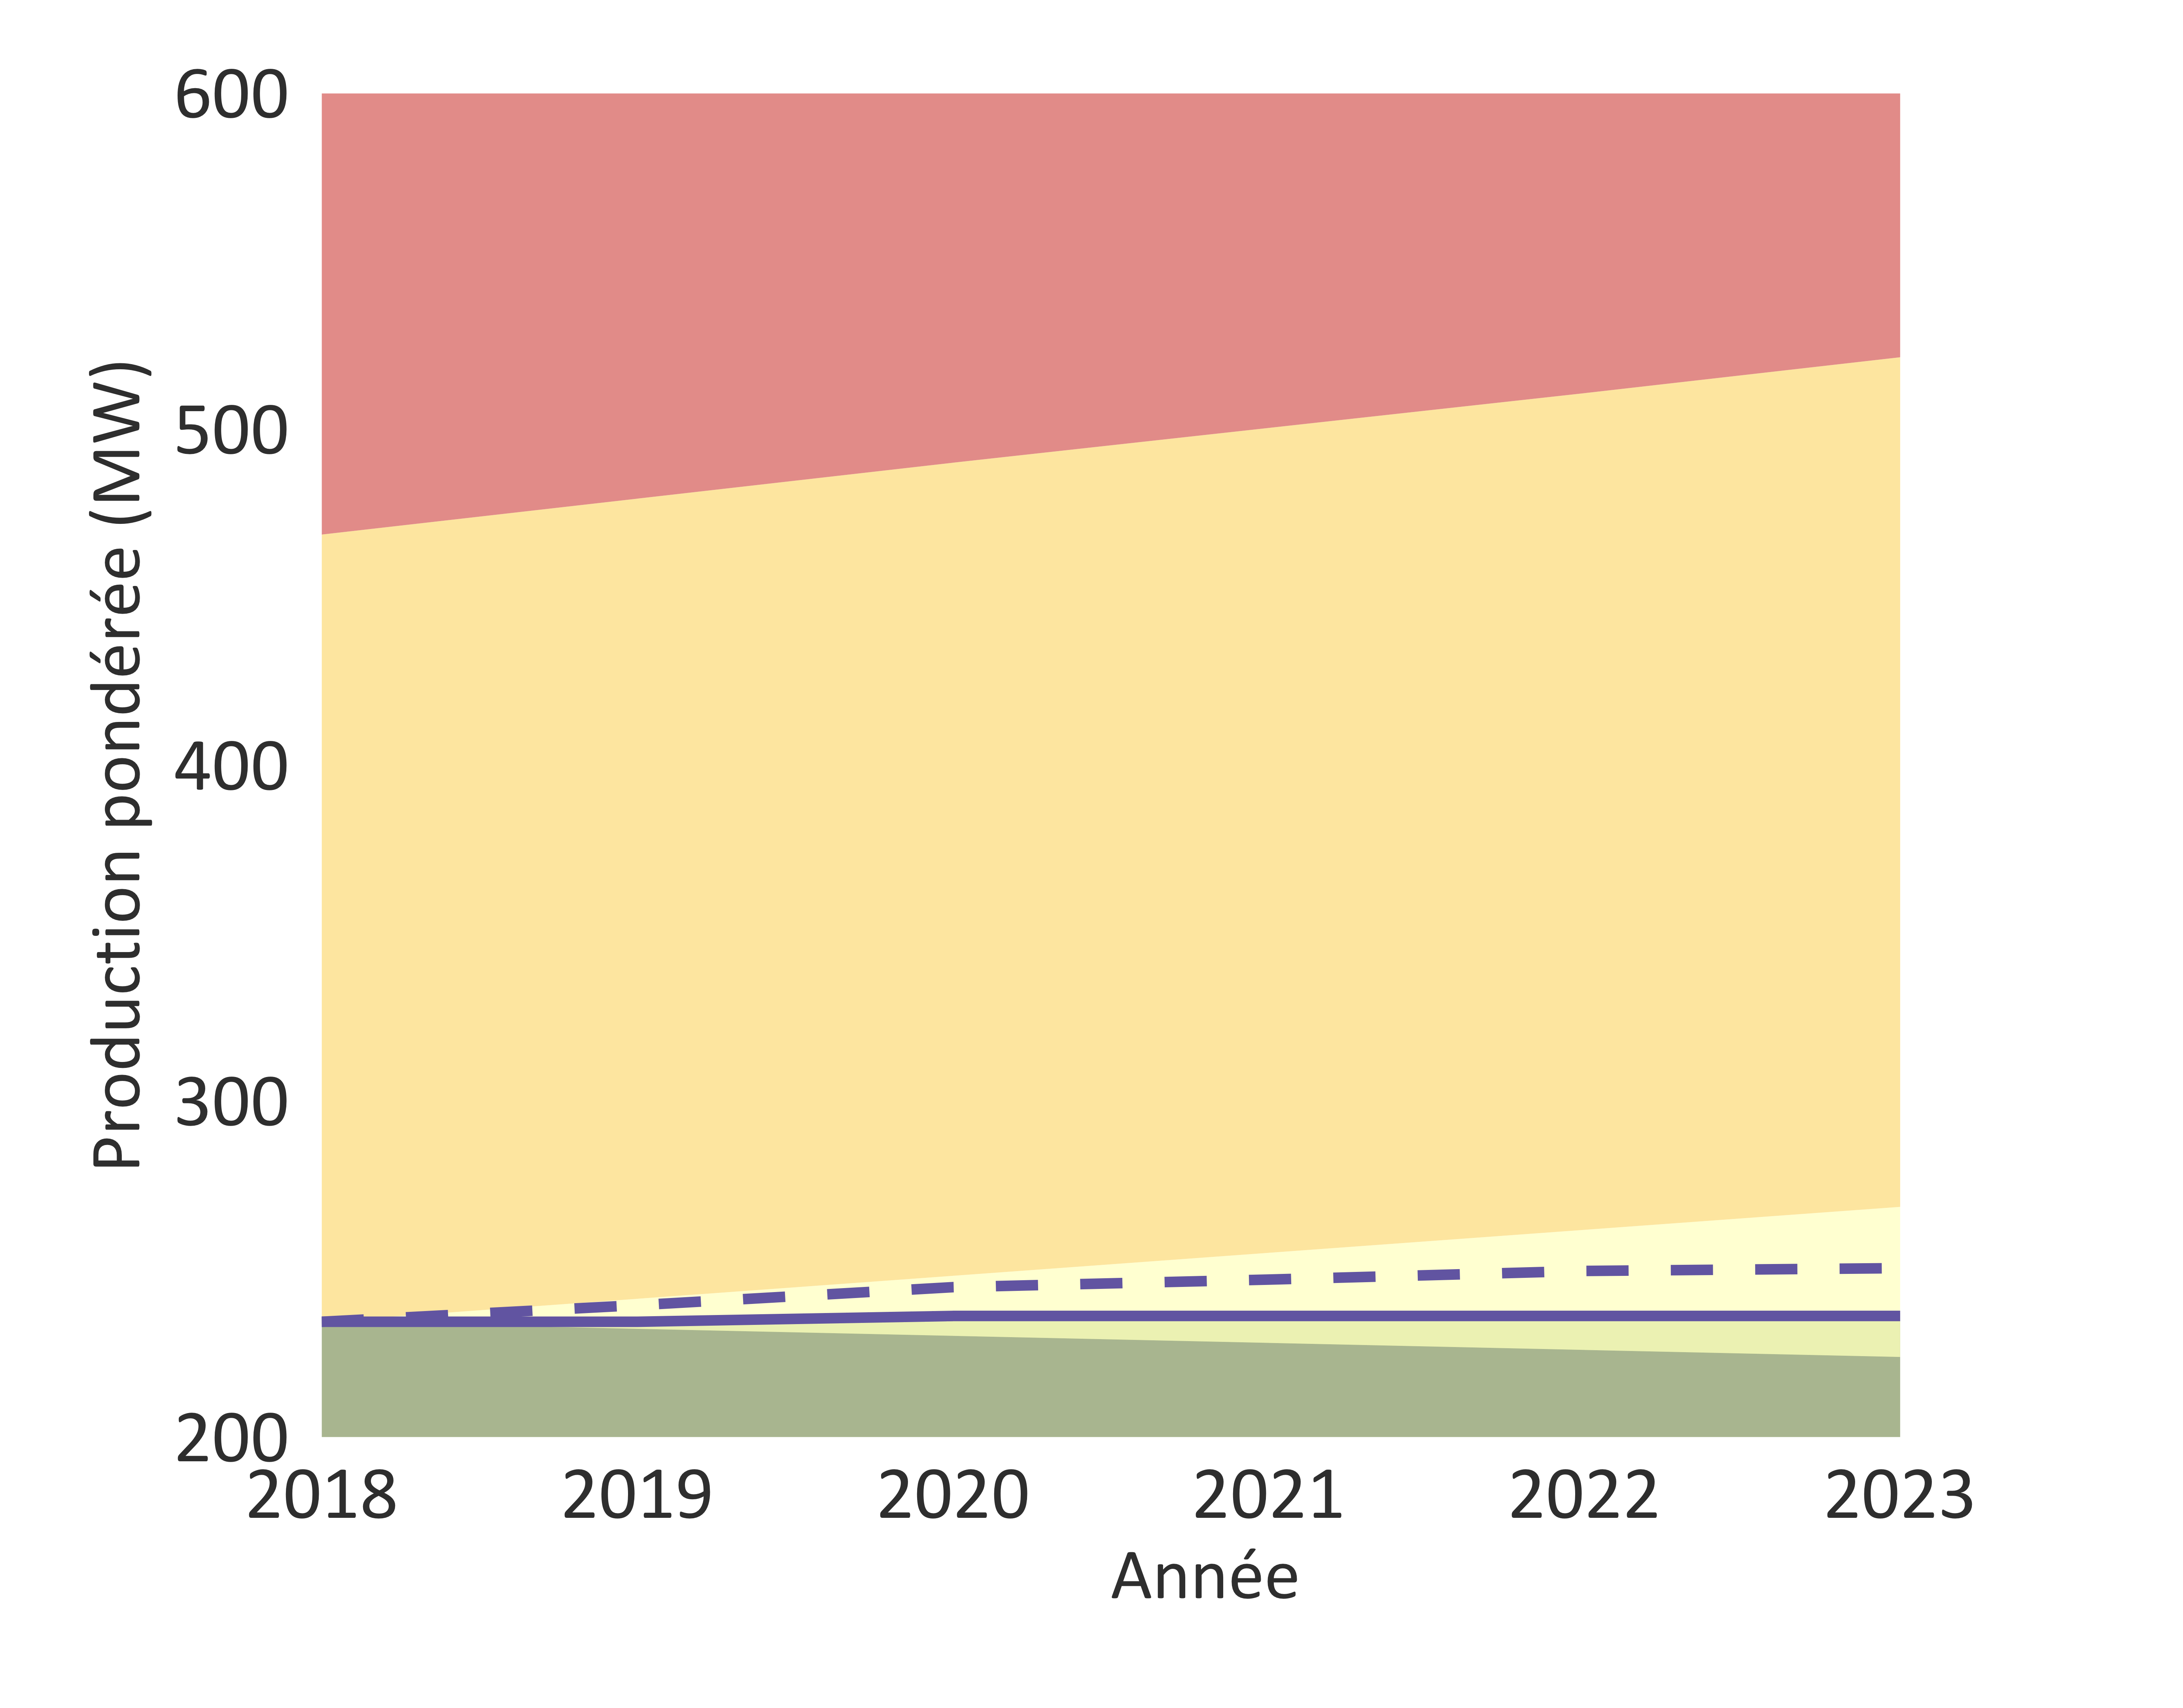
\includegraphics[trim = {0 0cm 0 0},width=1\linewidth]{ReportOutputs/Fig07}
		
		\textbf{Trayectoria de Capacidad Eléctrica de Renovables* }
		
		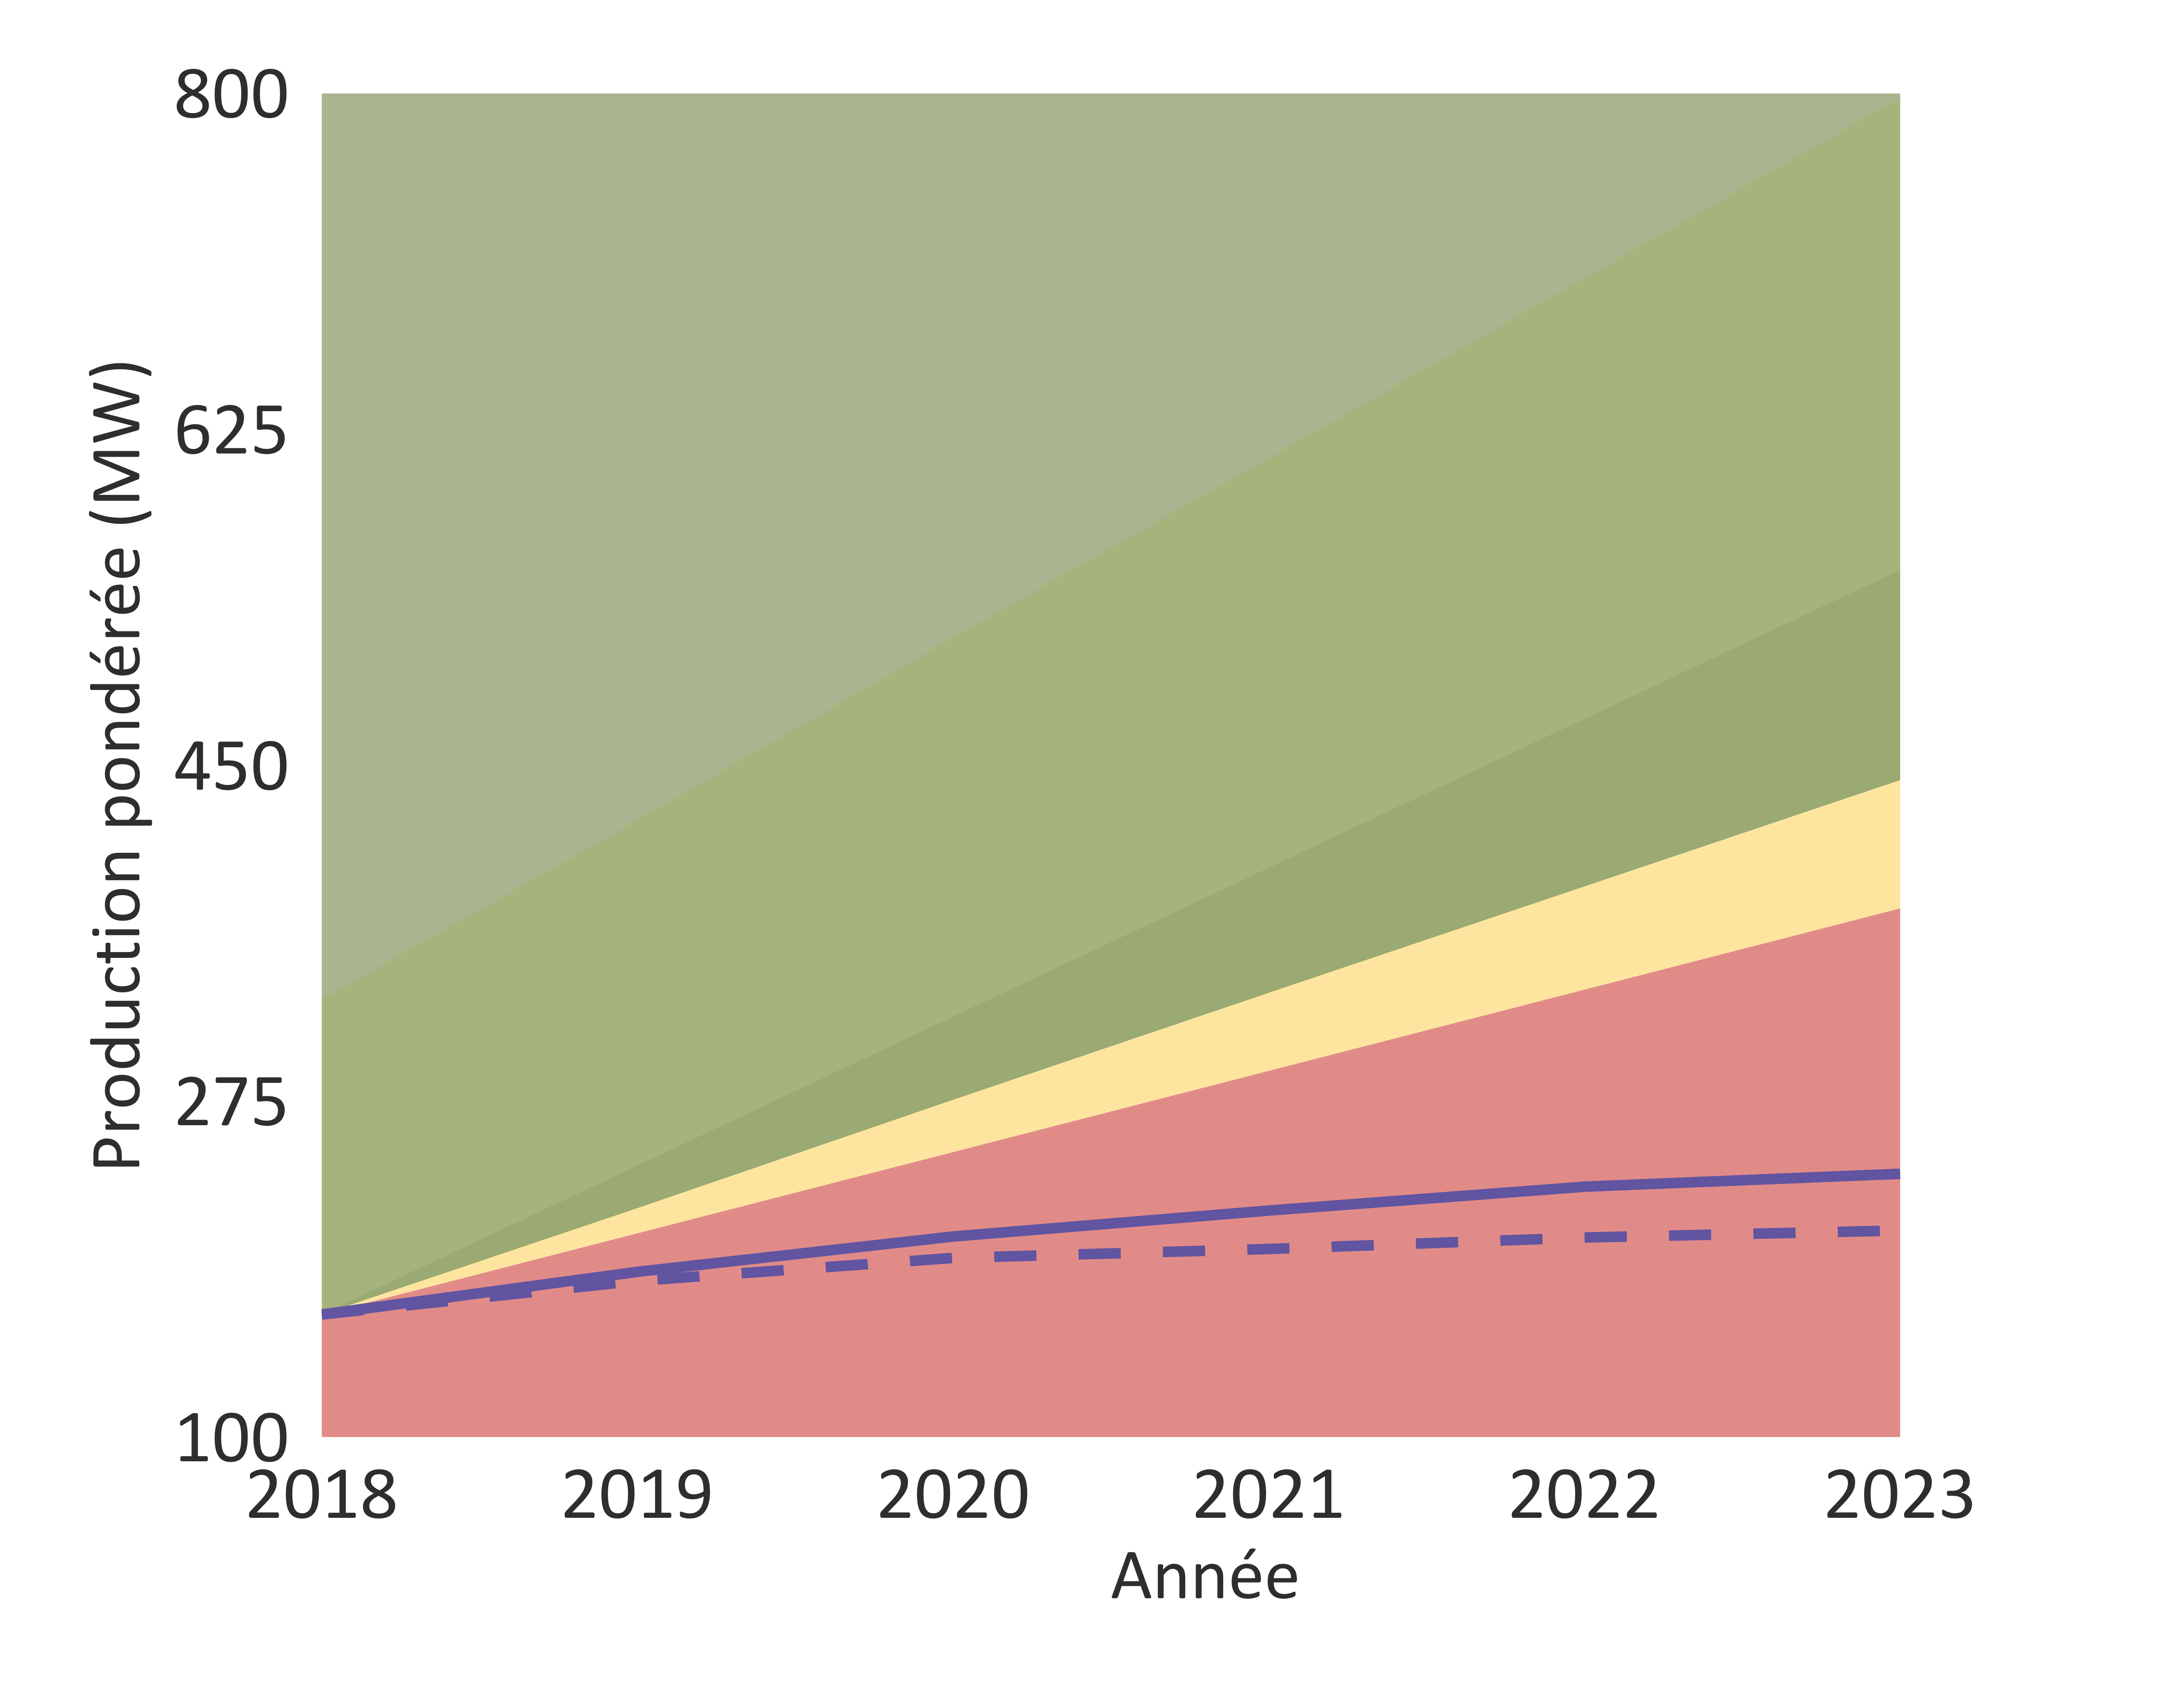
\includegraphics[trim = {0 0cm 0 0},width=.99\linewidth]{ReportOutputs/Fig08}
	\end{minipage}	
	\hspace{.02\linewidth}
	\begin{minipage}[t]{.49\textwidth}
		\textbf{Trayectoria de Capacidad Eléctrica de Gas }
		
		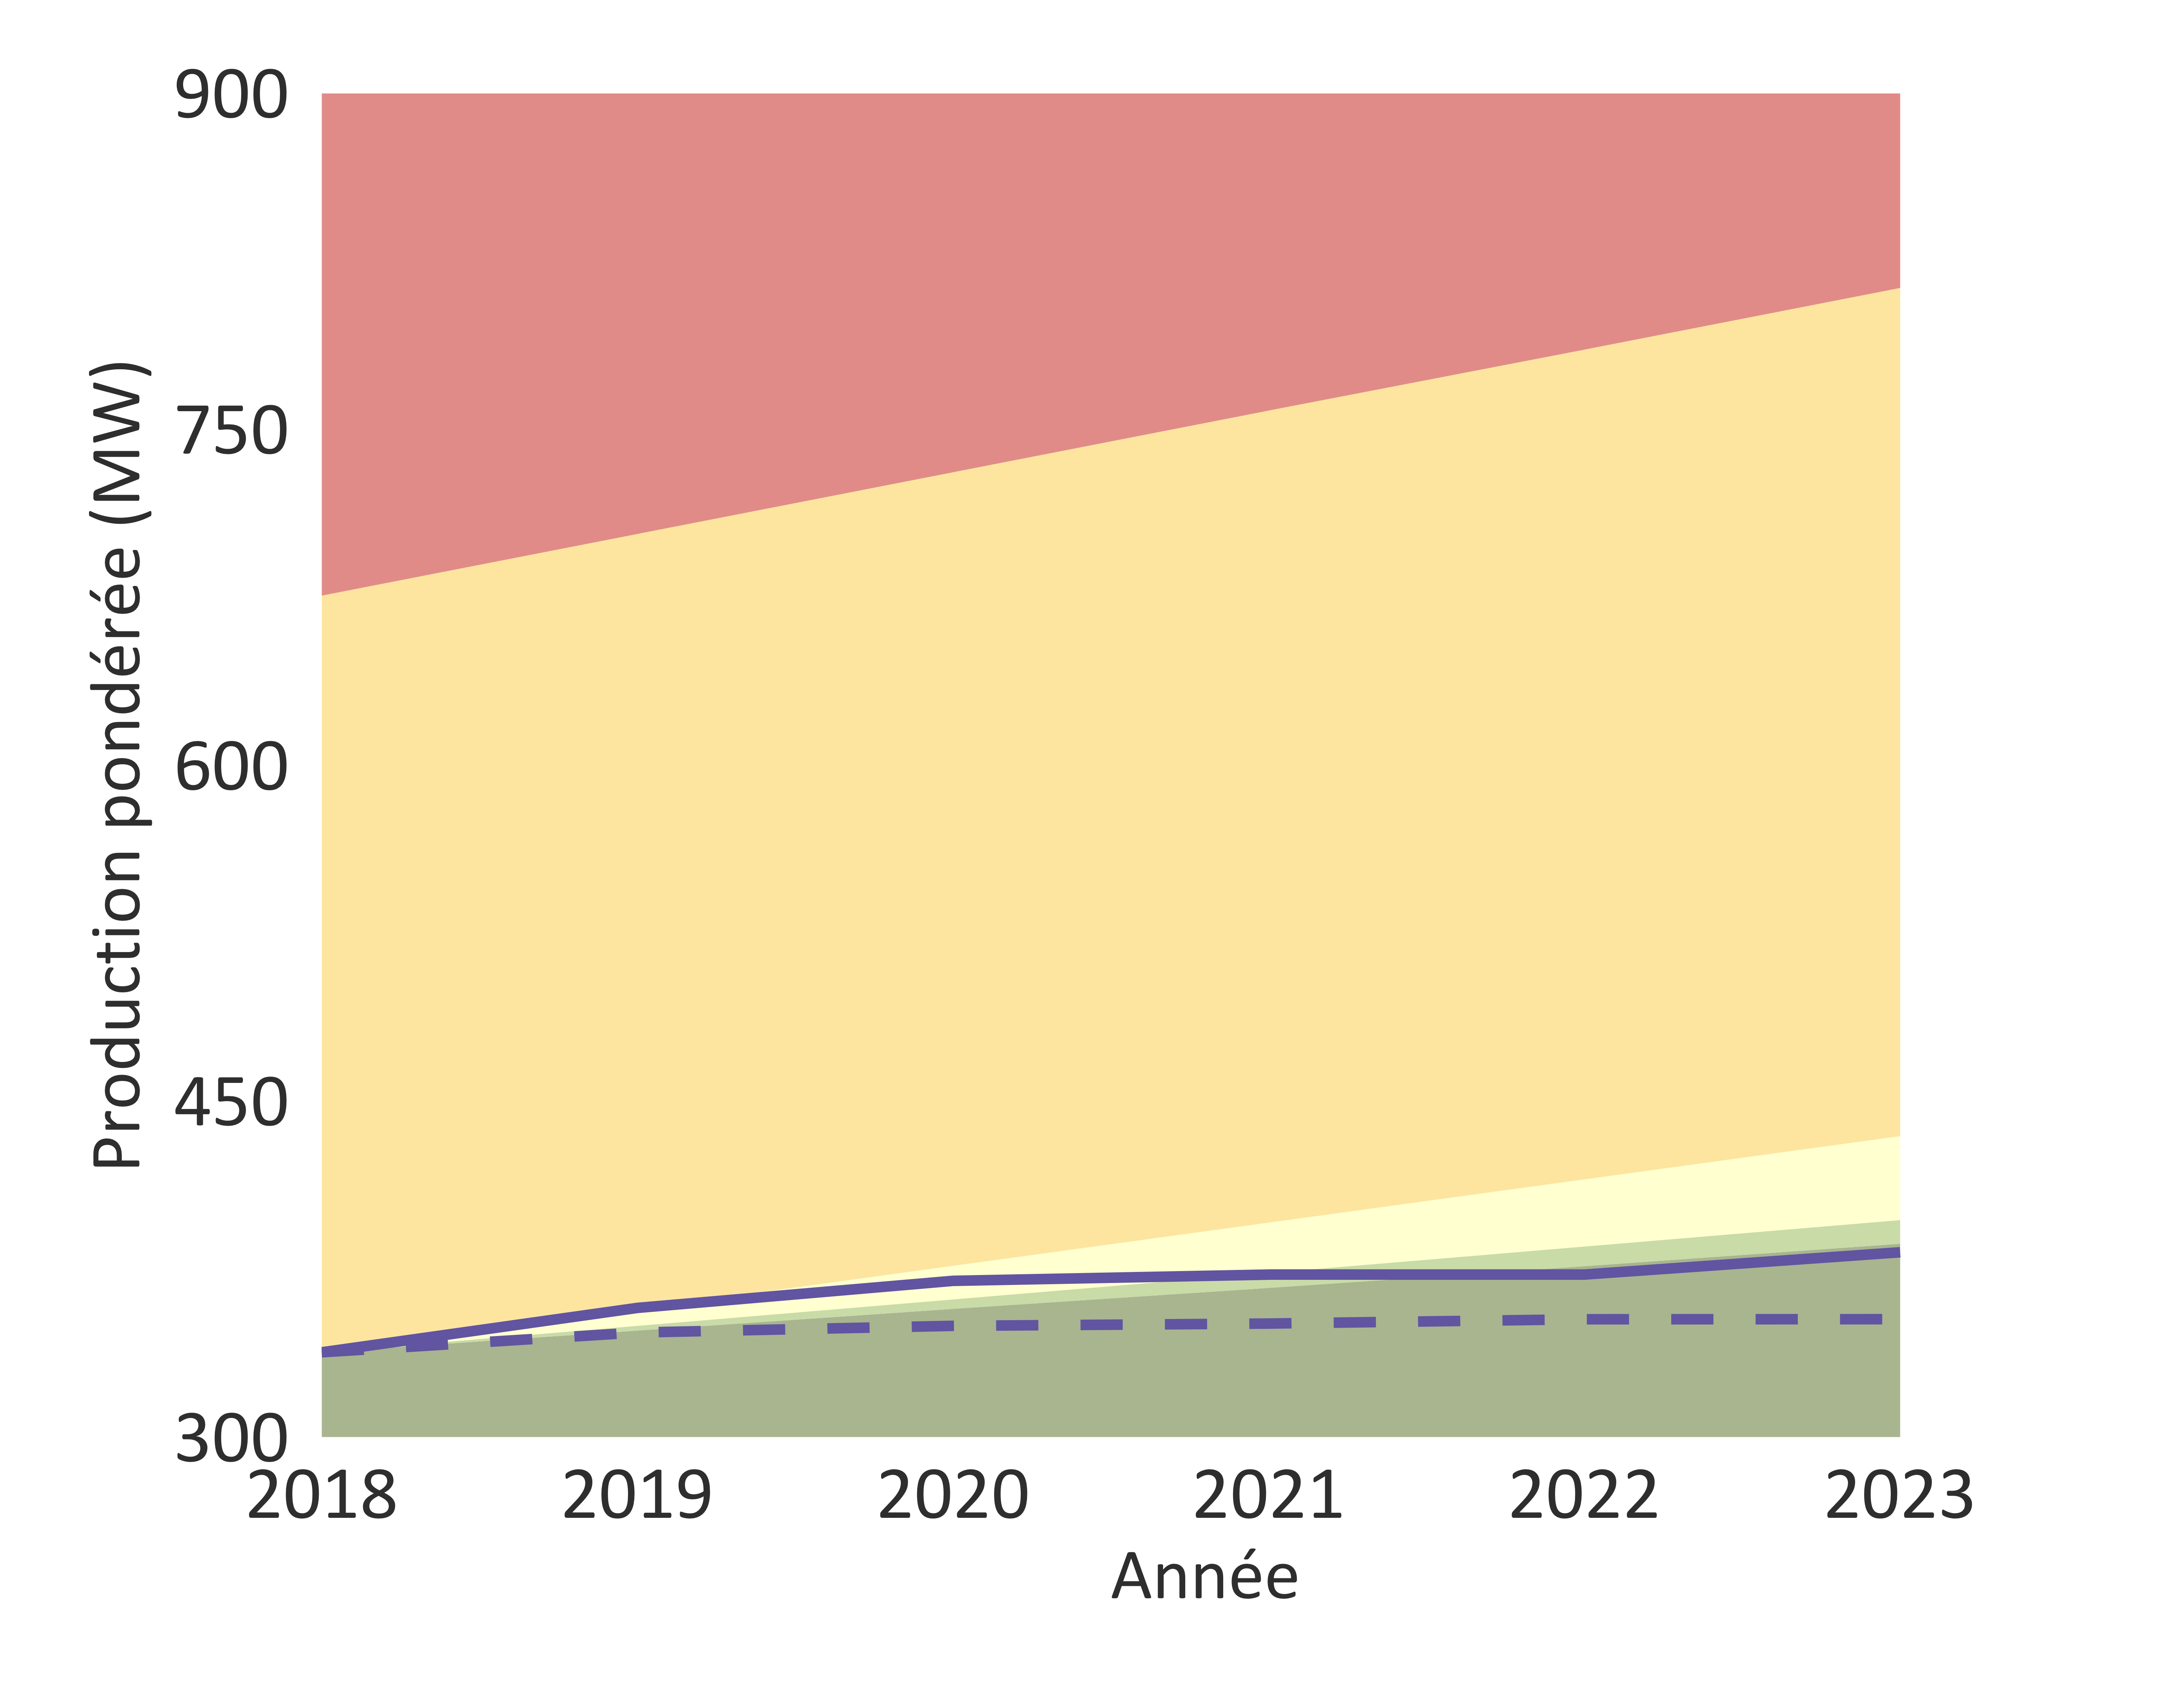
\includegraphics[trim = {0 0cm 0 0},width=1\linewidth]{ReportOutputs/Fig09}
		
		%WWFSpecificExcludeS
		\textbf{Trayectoria de Capacidad Eléctrica de Hidro}
		
		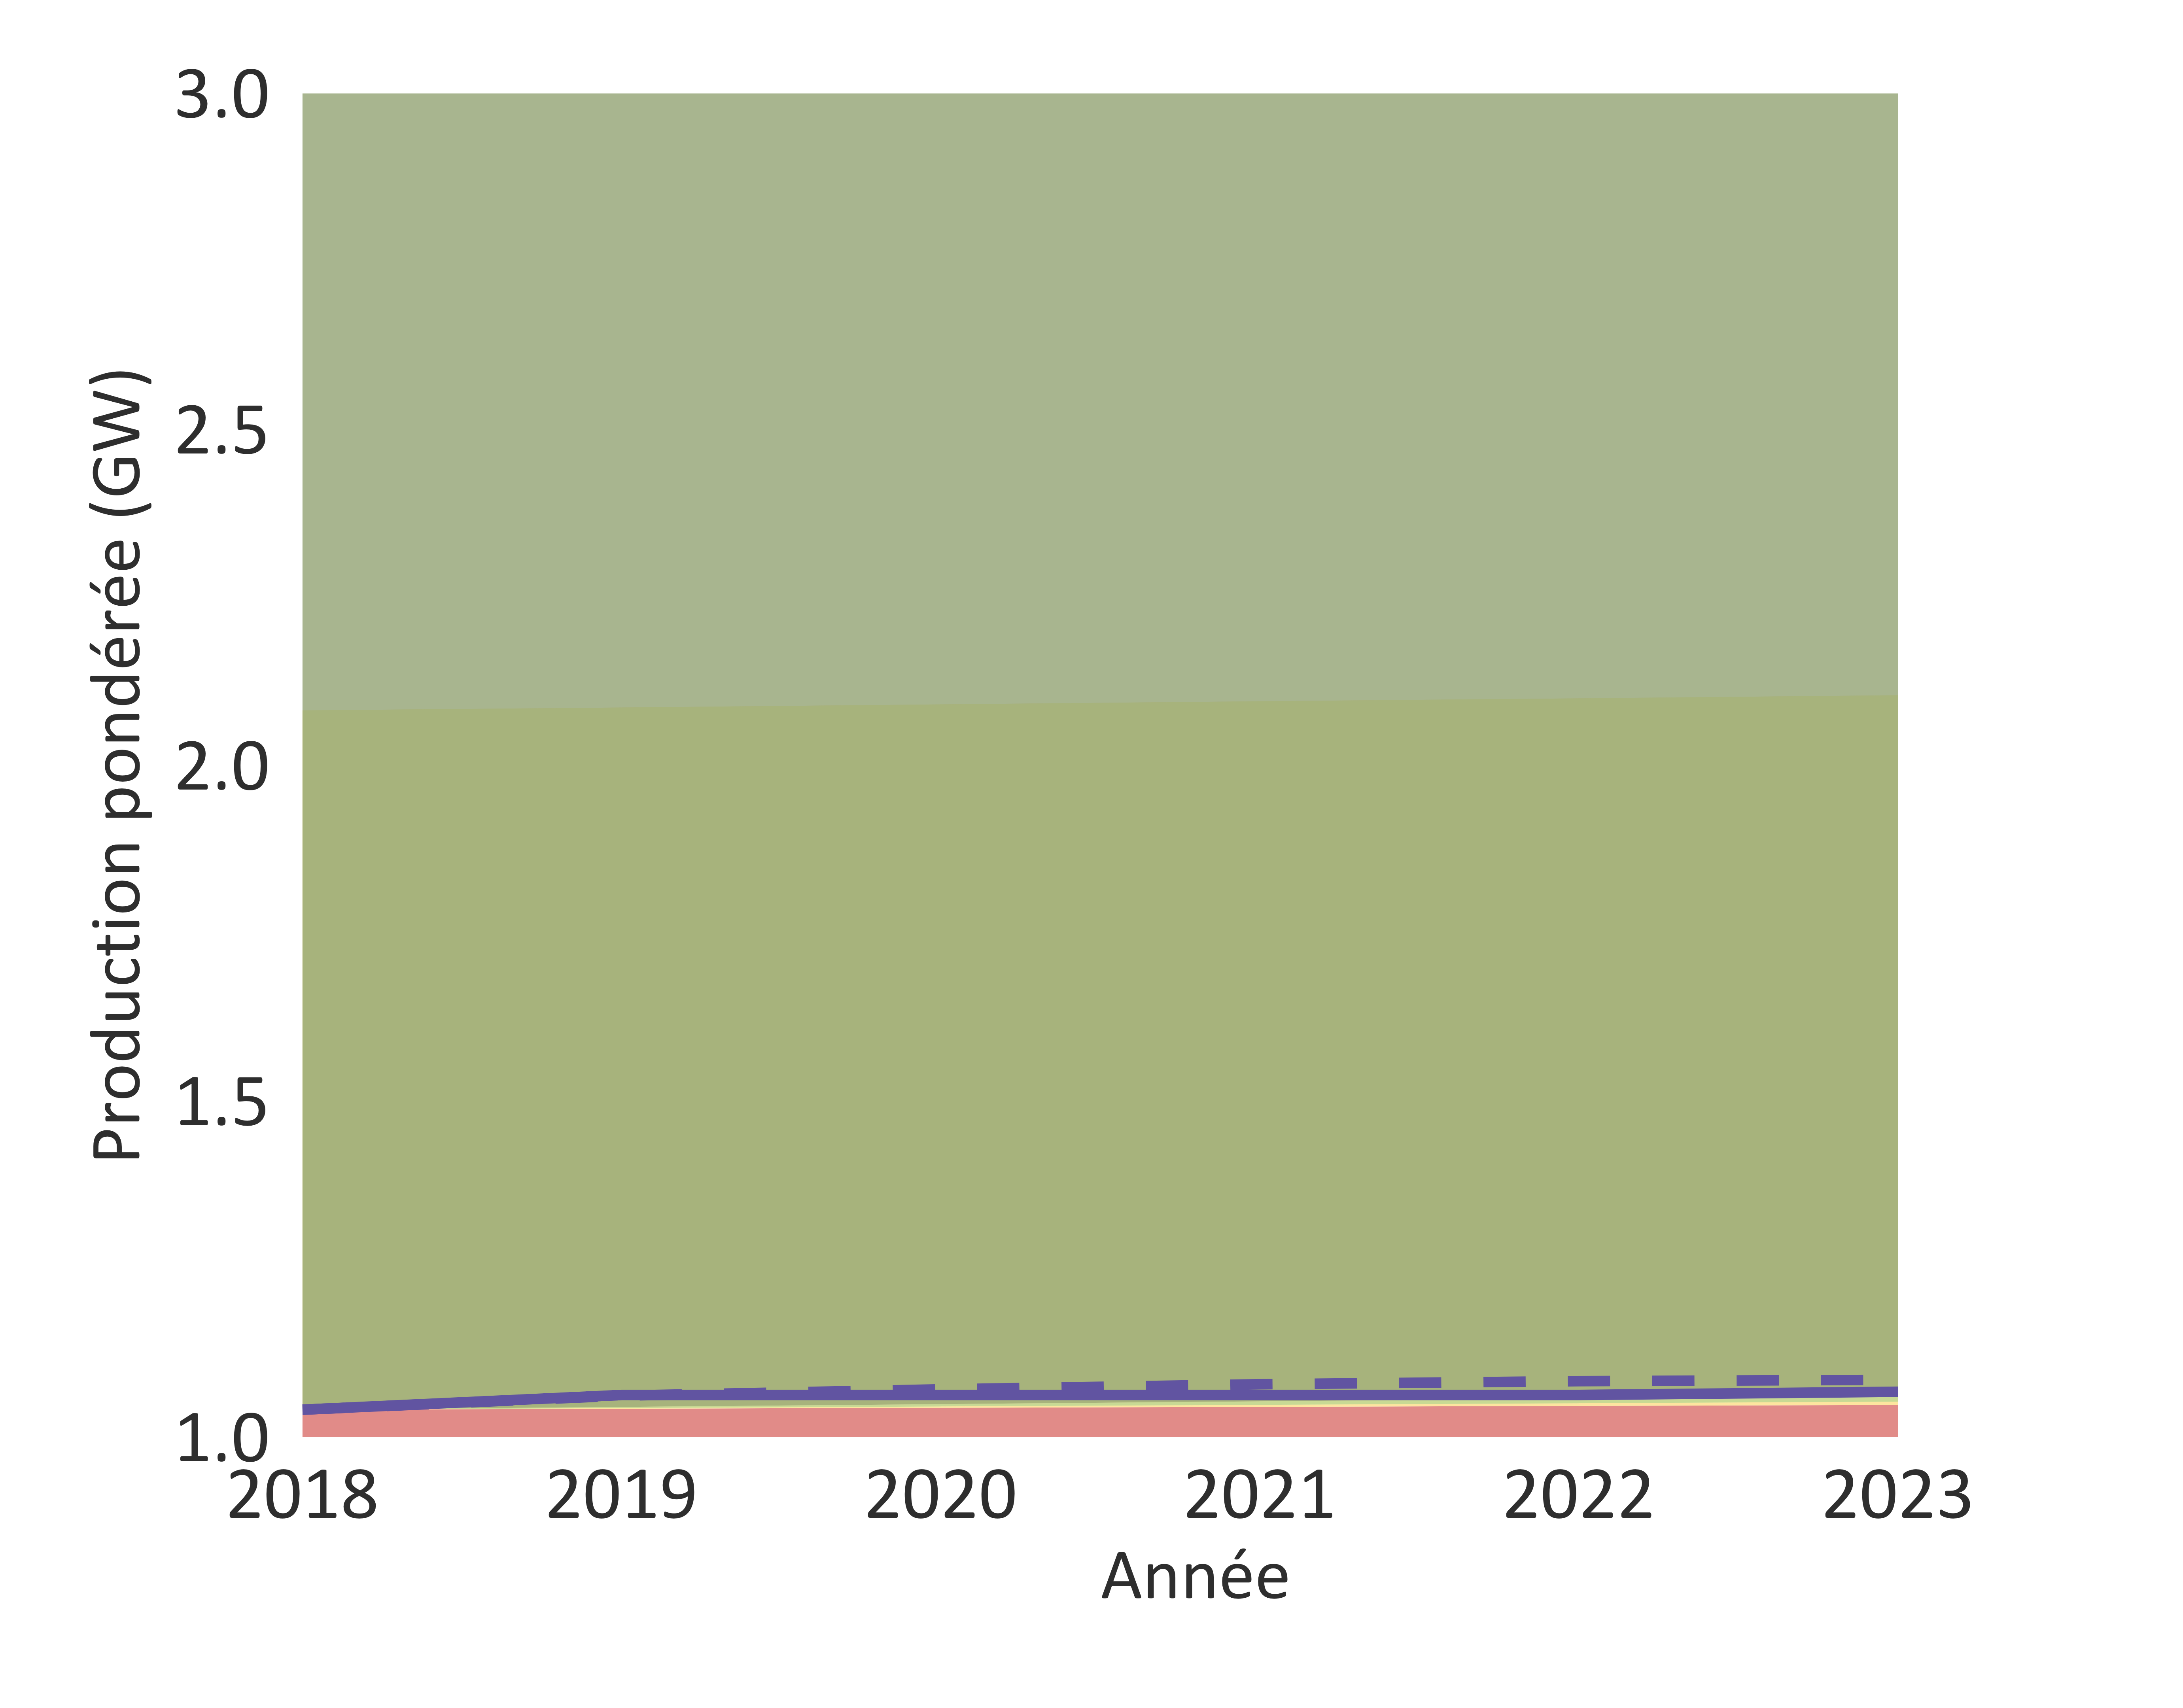
\includegraphics[trim = {0 0cm 0 0},width=1\linewidth]{ReportOutputs/Fig10}
		%WWFSpecificExcludeE
		
	\end{minipage}
	
	\vspace{-0.8cm}
	\begin{center}
		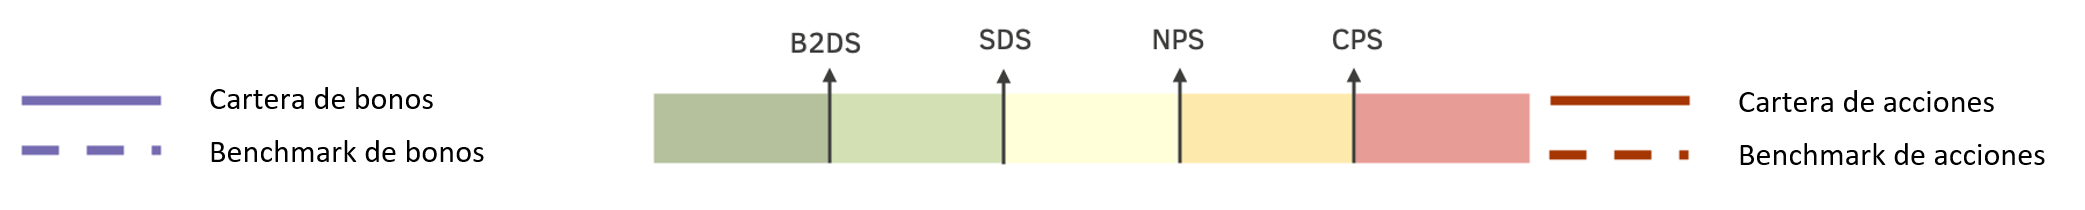
\includegraphics[trim = {0 0cm 0 0},width=.9\linewidth]{ReportGraphics/246Legend_ES.png}
	\end{center}
	
	\small\textit{*Debido a diferentes supuestos en los escenarios B2DS y SDS sobre la  combinación tecnológica esperada en el sector de energías renovables, el escenario SDS puede parecer más ambicioso que el B2DS. Sin embargo, en el escenario B2DS se espera que la generación de energía renovable sea mayor a la del SDS a pesar de que la capacidad sea menor.}
	
	%\PageFooterThird
\PageFooter{3 - TRAYECTORIA DE LA CARTERA}
	\newpage 
	%PowerSector_CBE
	%PowerSector_EQS
	\section*{} % TRAJECTORY - EQUITY - POWER  
	\HeaderDouble{TENDENCIA DE 5 AÑOS – ACCIONES}{SECTOR ELÉCTRICO}		
	
	\begin{multicols}{2}
		\textbf{Los gráficos de alineación a continuación muestran la alineación de tecnologías en el sector eléctrico de la cartera de acciones respecto a los escenarios de transición de la AIE: B2DS, SDS, NPS, CPS y la alineación del mercado de acciones.} 
		Para cada tecnología, el valor graficado de la cartera (línea continua) representa la evolución planeada o “trayectoria” de la capacidad instalada atribuida a la cartera acciones en los próximos 5 años.        
		Las líneas que separan las áreas del fondo codificado por colores representan la “producción objetivo” de la cartera para cada tecnología bajo los escenarios de la AIE. La línea punteada muestra la trayectoria planeada de la capacidad instalada para cada tecnología en el mercado de acciones, ajustada al mismo punto de inicio de la cartera.        
		
	\end{multicols}
	
	\vspace{-0.5cm}
	
	\begin{minipage}[t]{.49\linewidth}
		\textbf{Trayectoria de Capacidad Eléctrica de Carbón}
		
		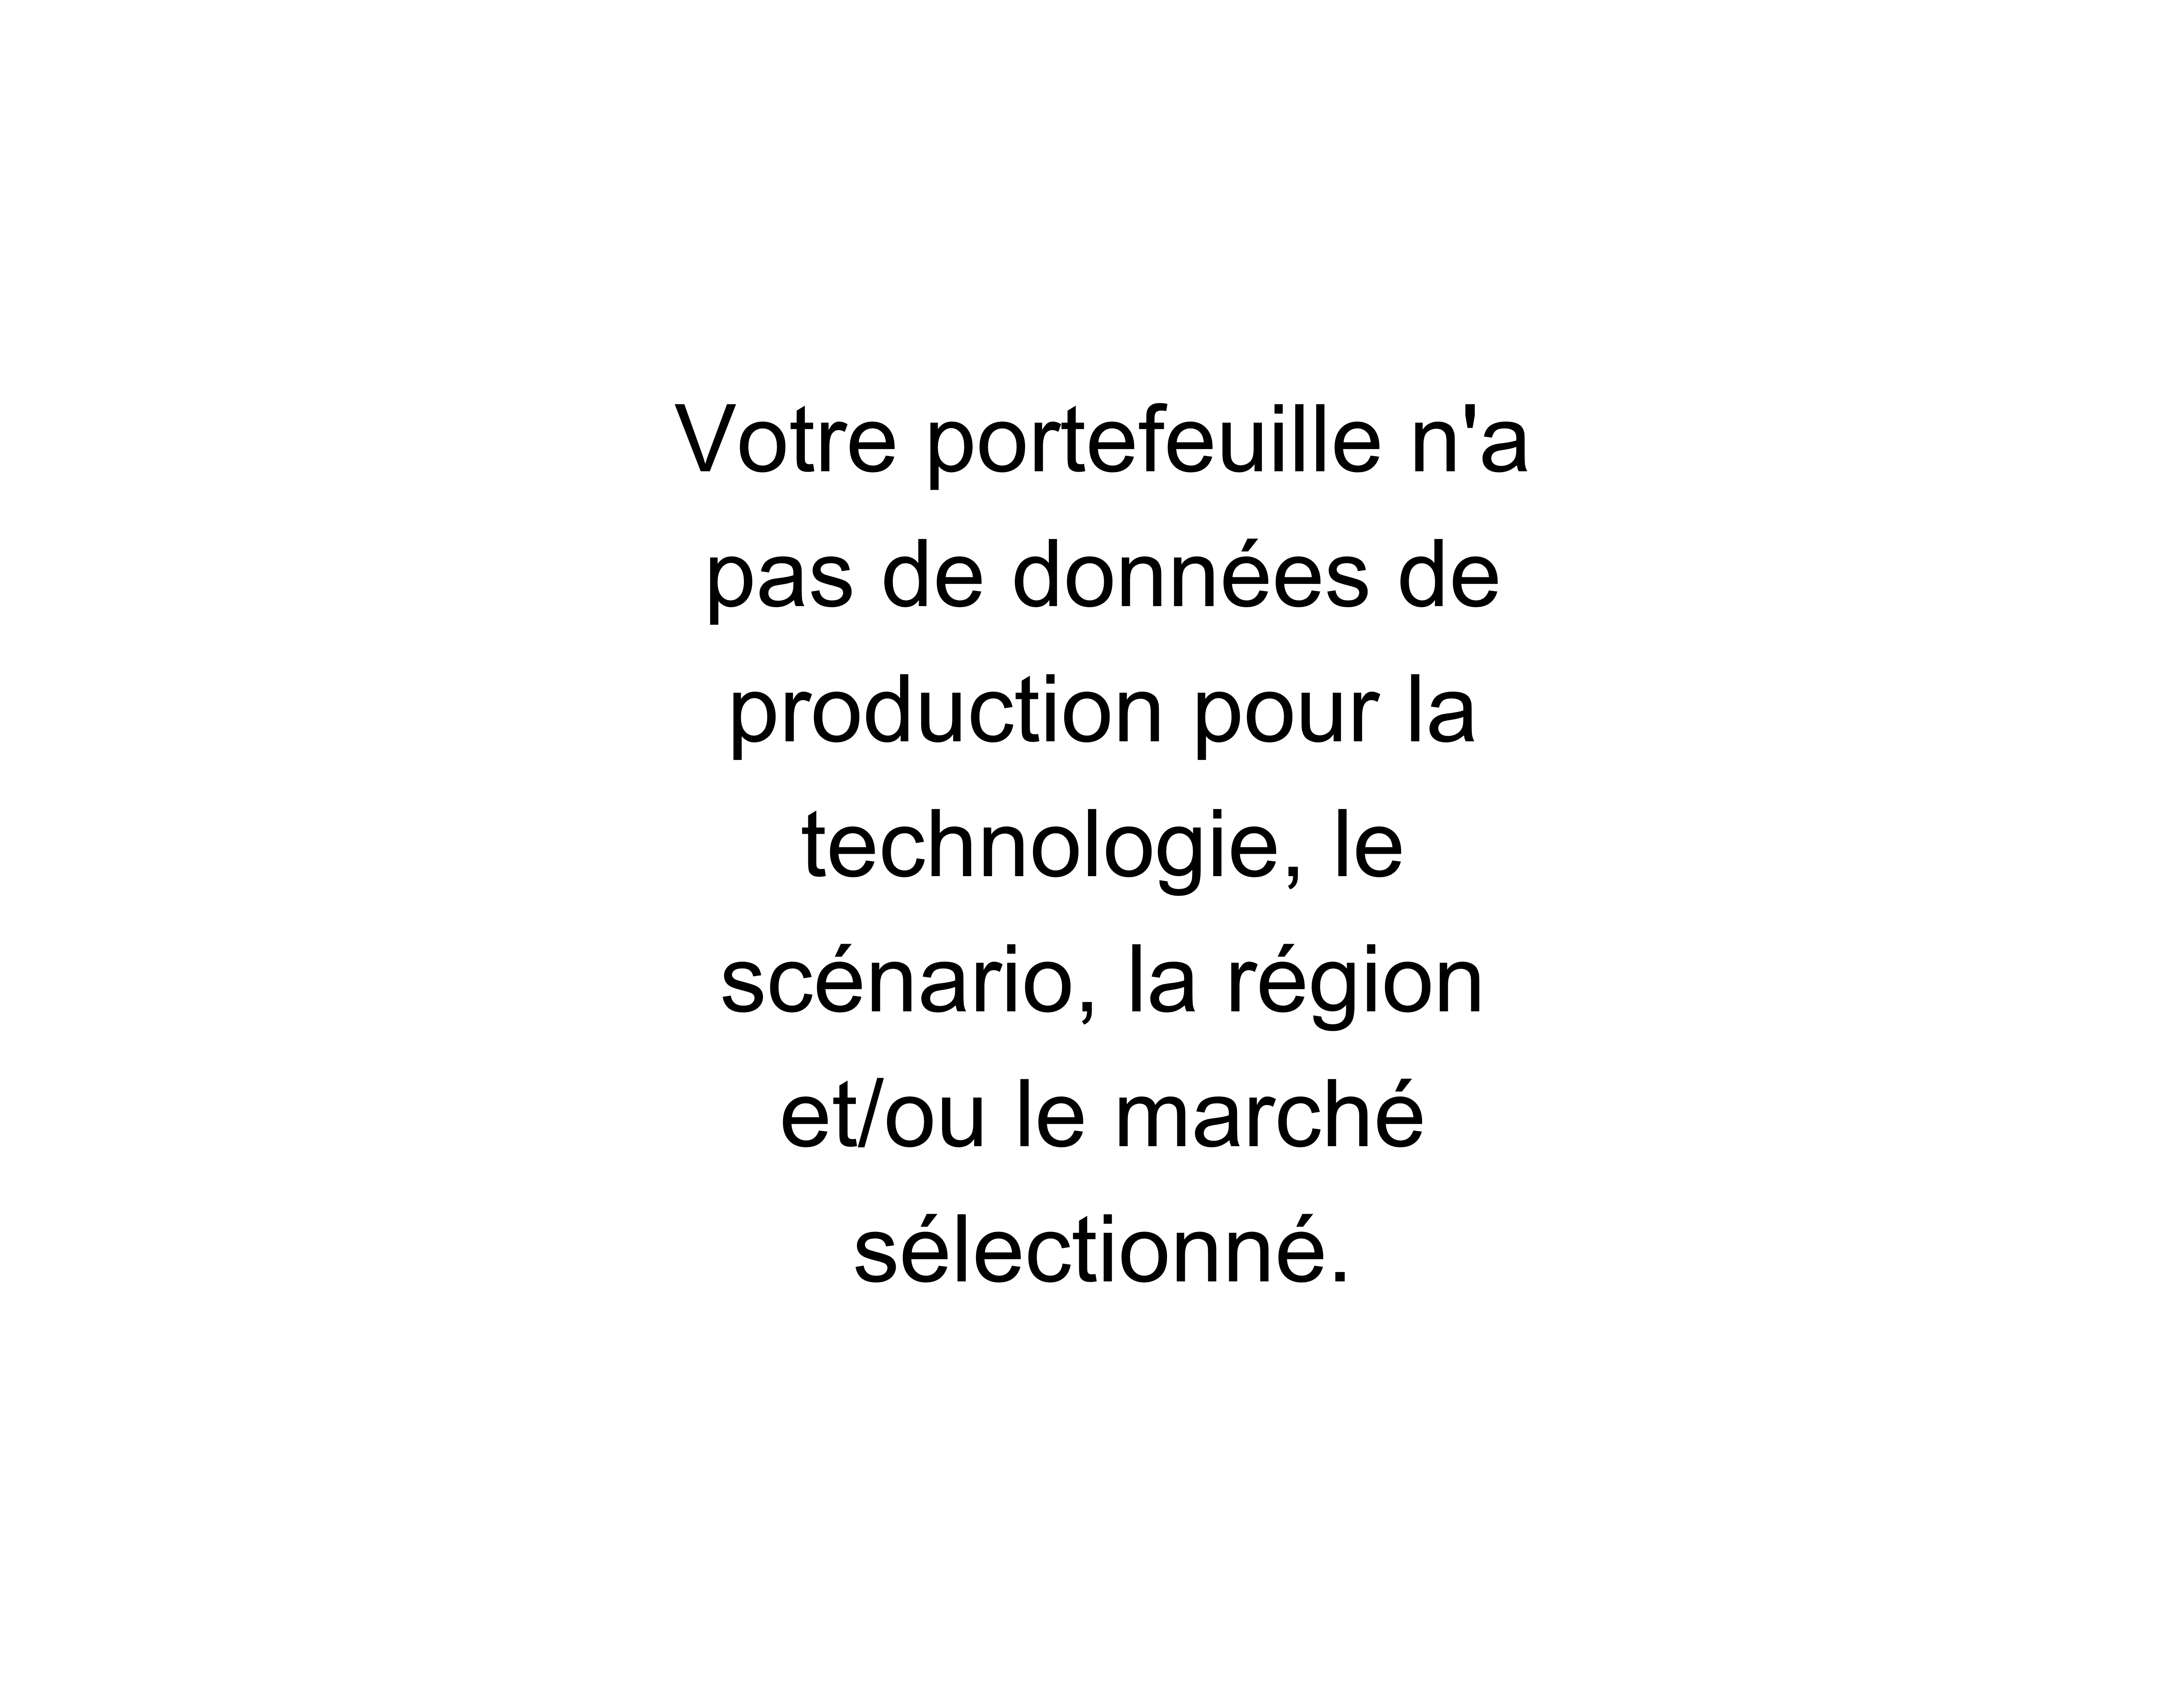
\includegraphics[trim = {0 0cm 0 0},width=1\linewidth]{ReportOutputs/Fig17}
		
		\textbf{Trayectoria de Capacidad Eléctrica de Renovables* }
		
		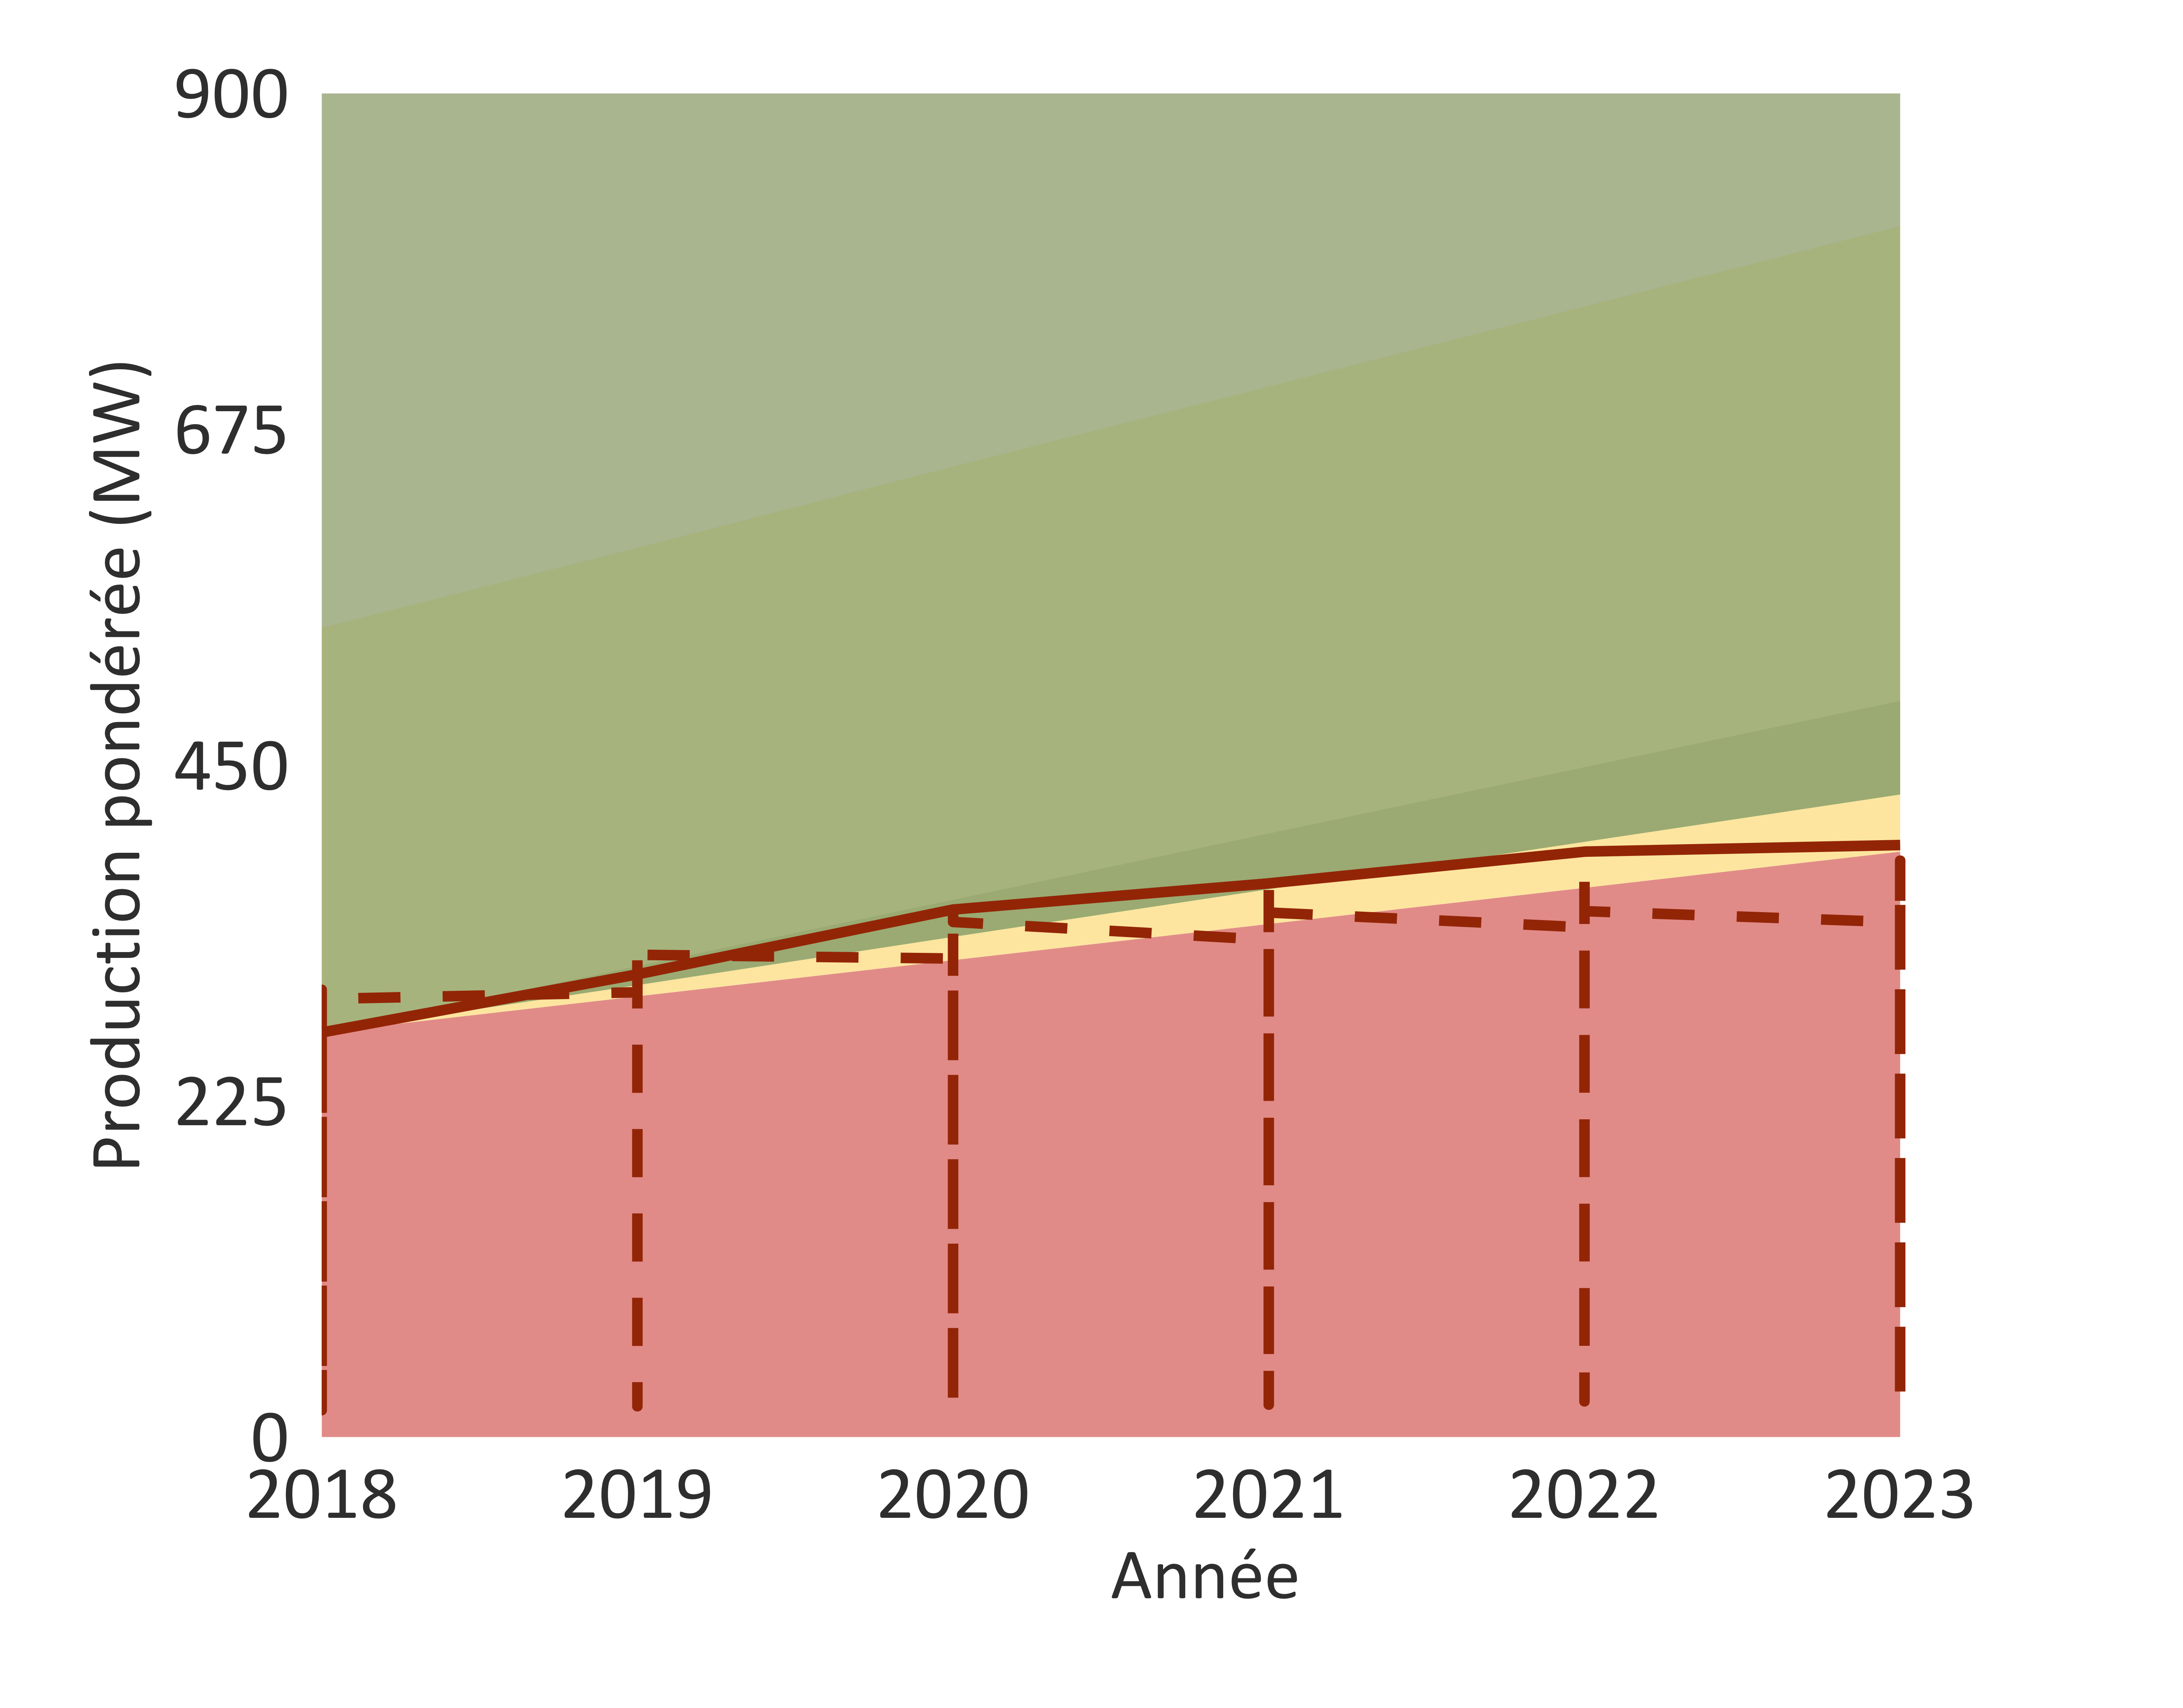
\includegraphics[trim = {0 0cm 0 0},width=.99\linewidth]{ReportOutputs/Fig18}
	\end{minipage}	
	\hspace{.02\linewidth}
	\begin{minipage}[t]{.49\textwidth}
		\textbf{Trayectoria de Capacidad Eléctrica de Gas }
		
		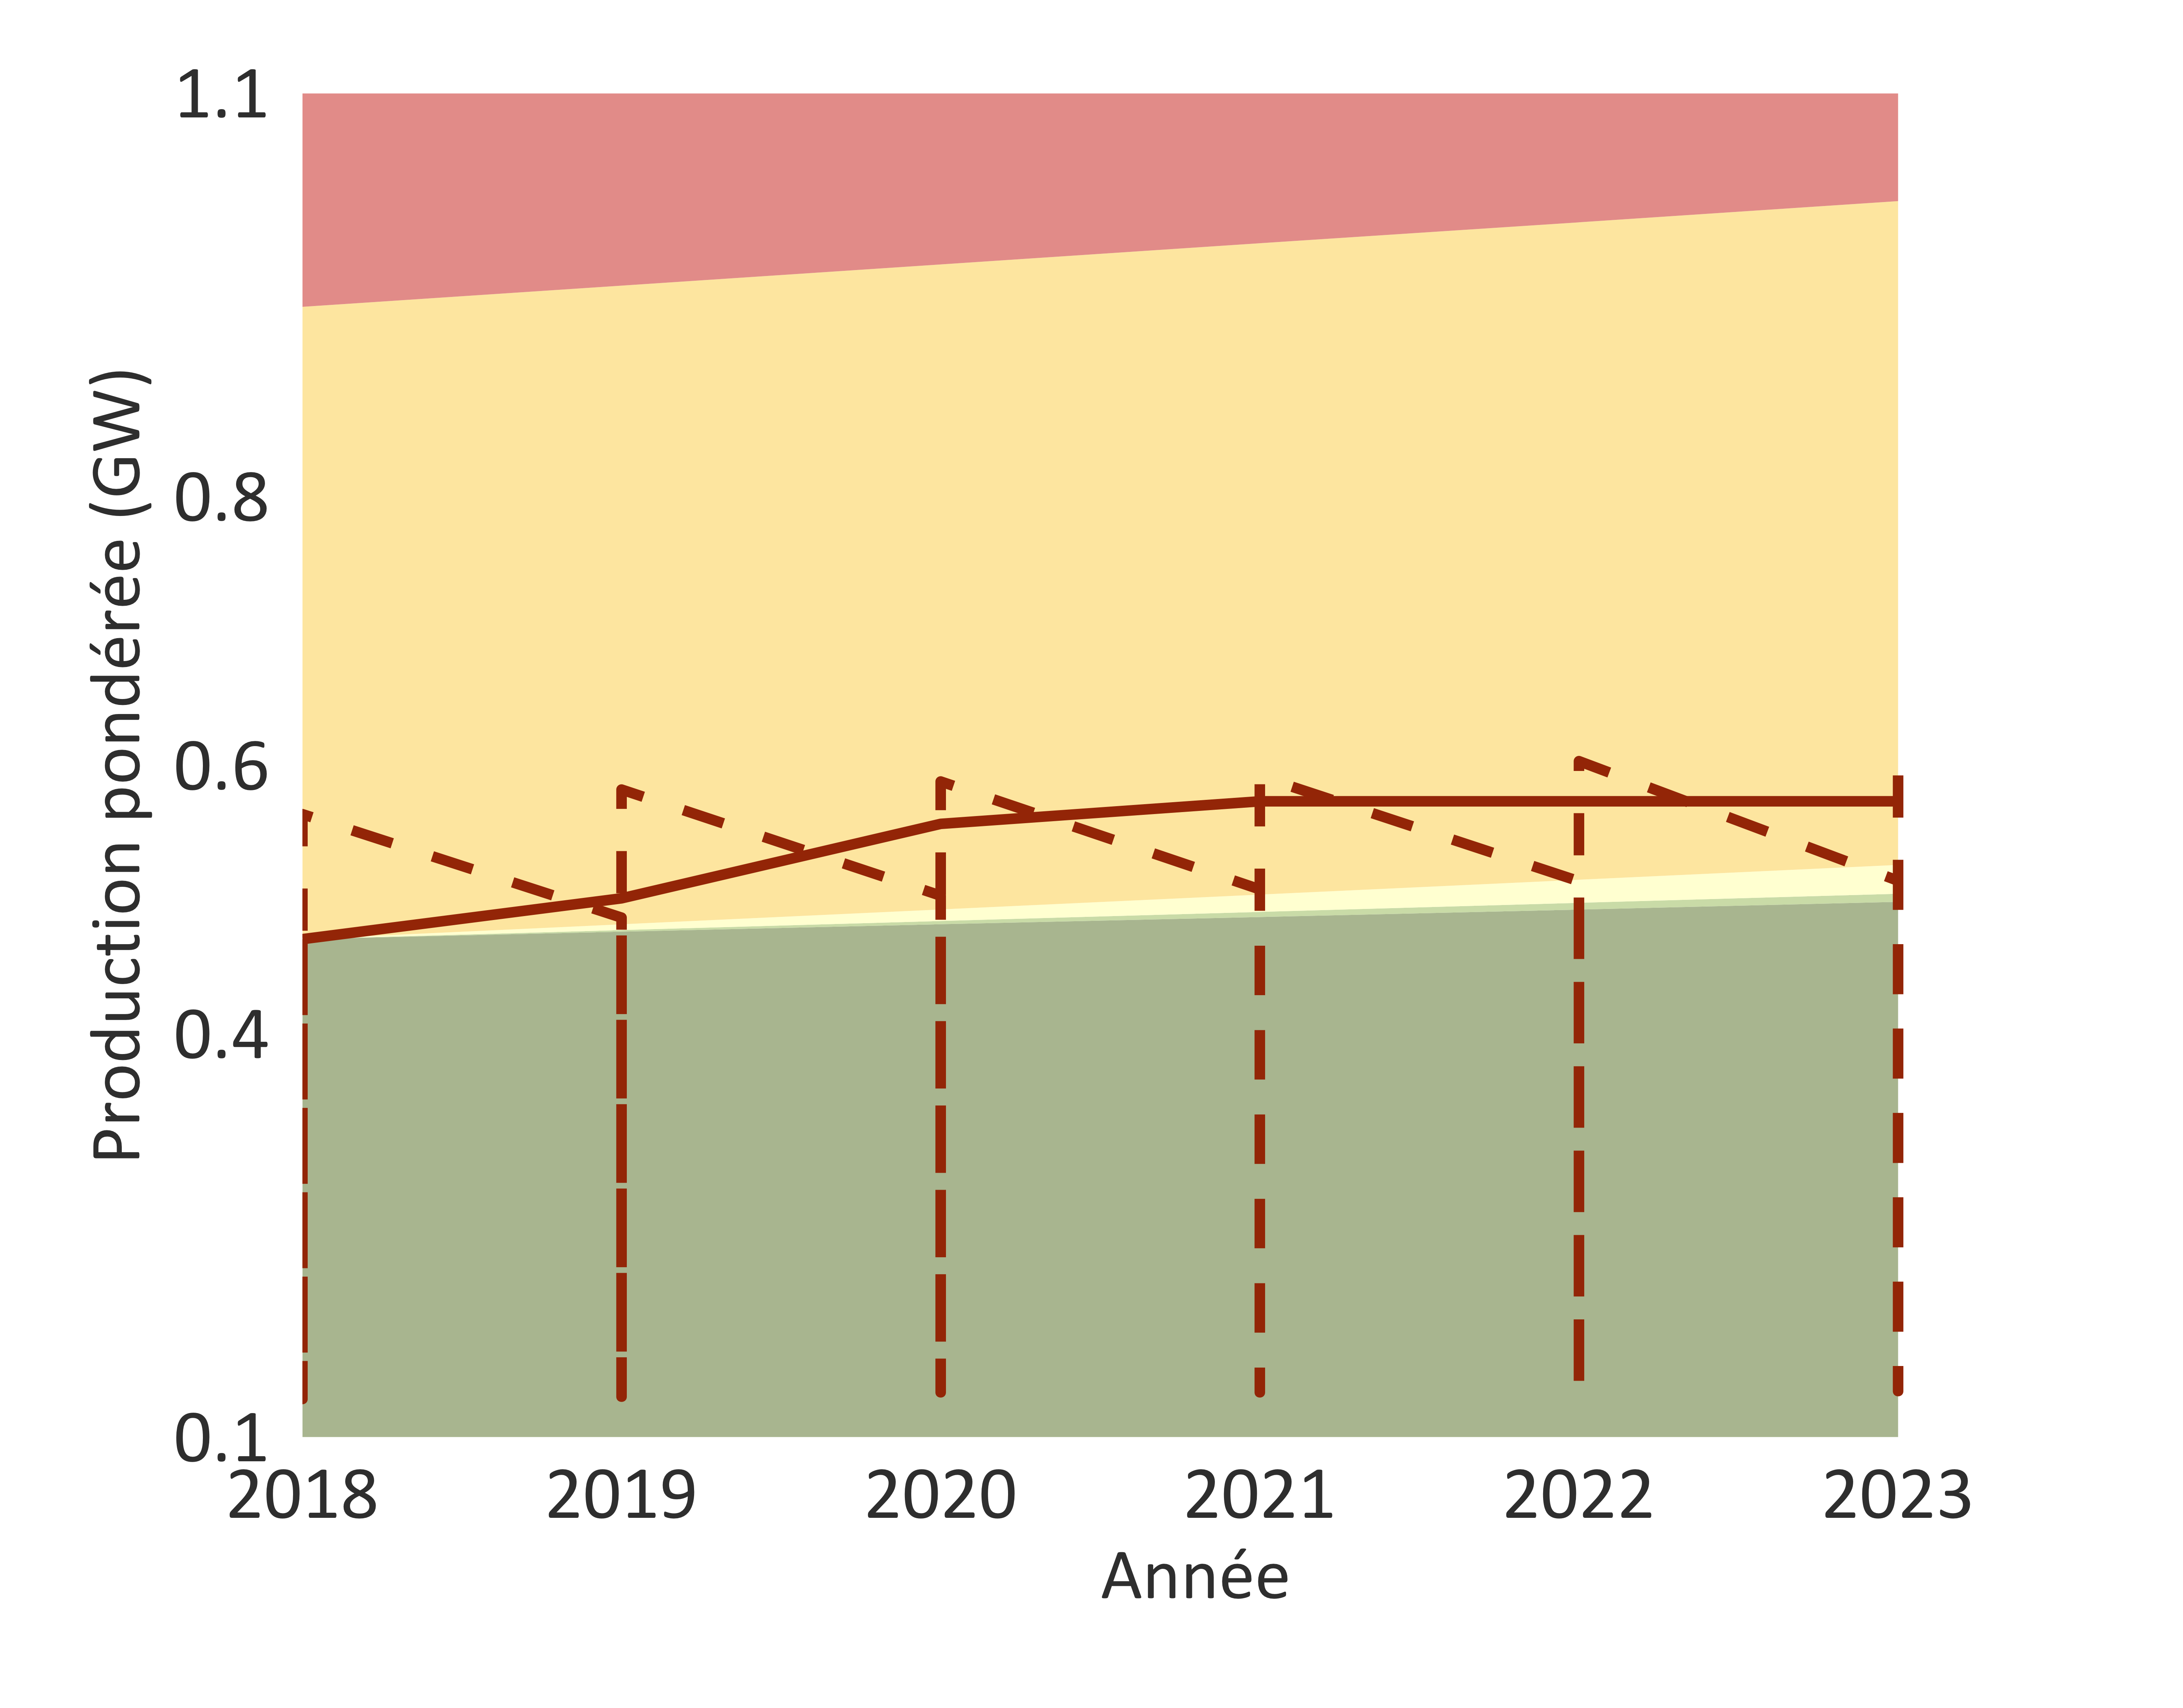
\includegraphics[trim = {0 0cm 0 0},width=1\linewidth]{ReportOutputs/Fig19}
		
		%WWFSpecificExcludeS
		\textbf{Trayectoria de Capacidad Eléctrica de Hidro }
		
		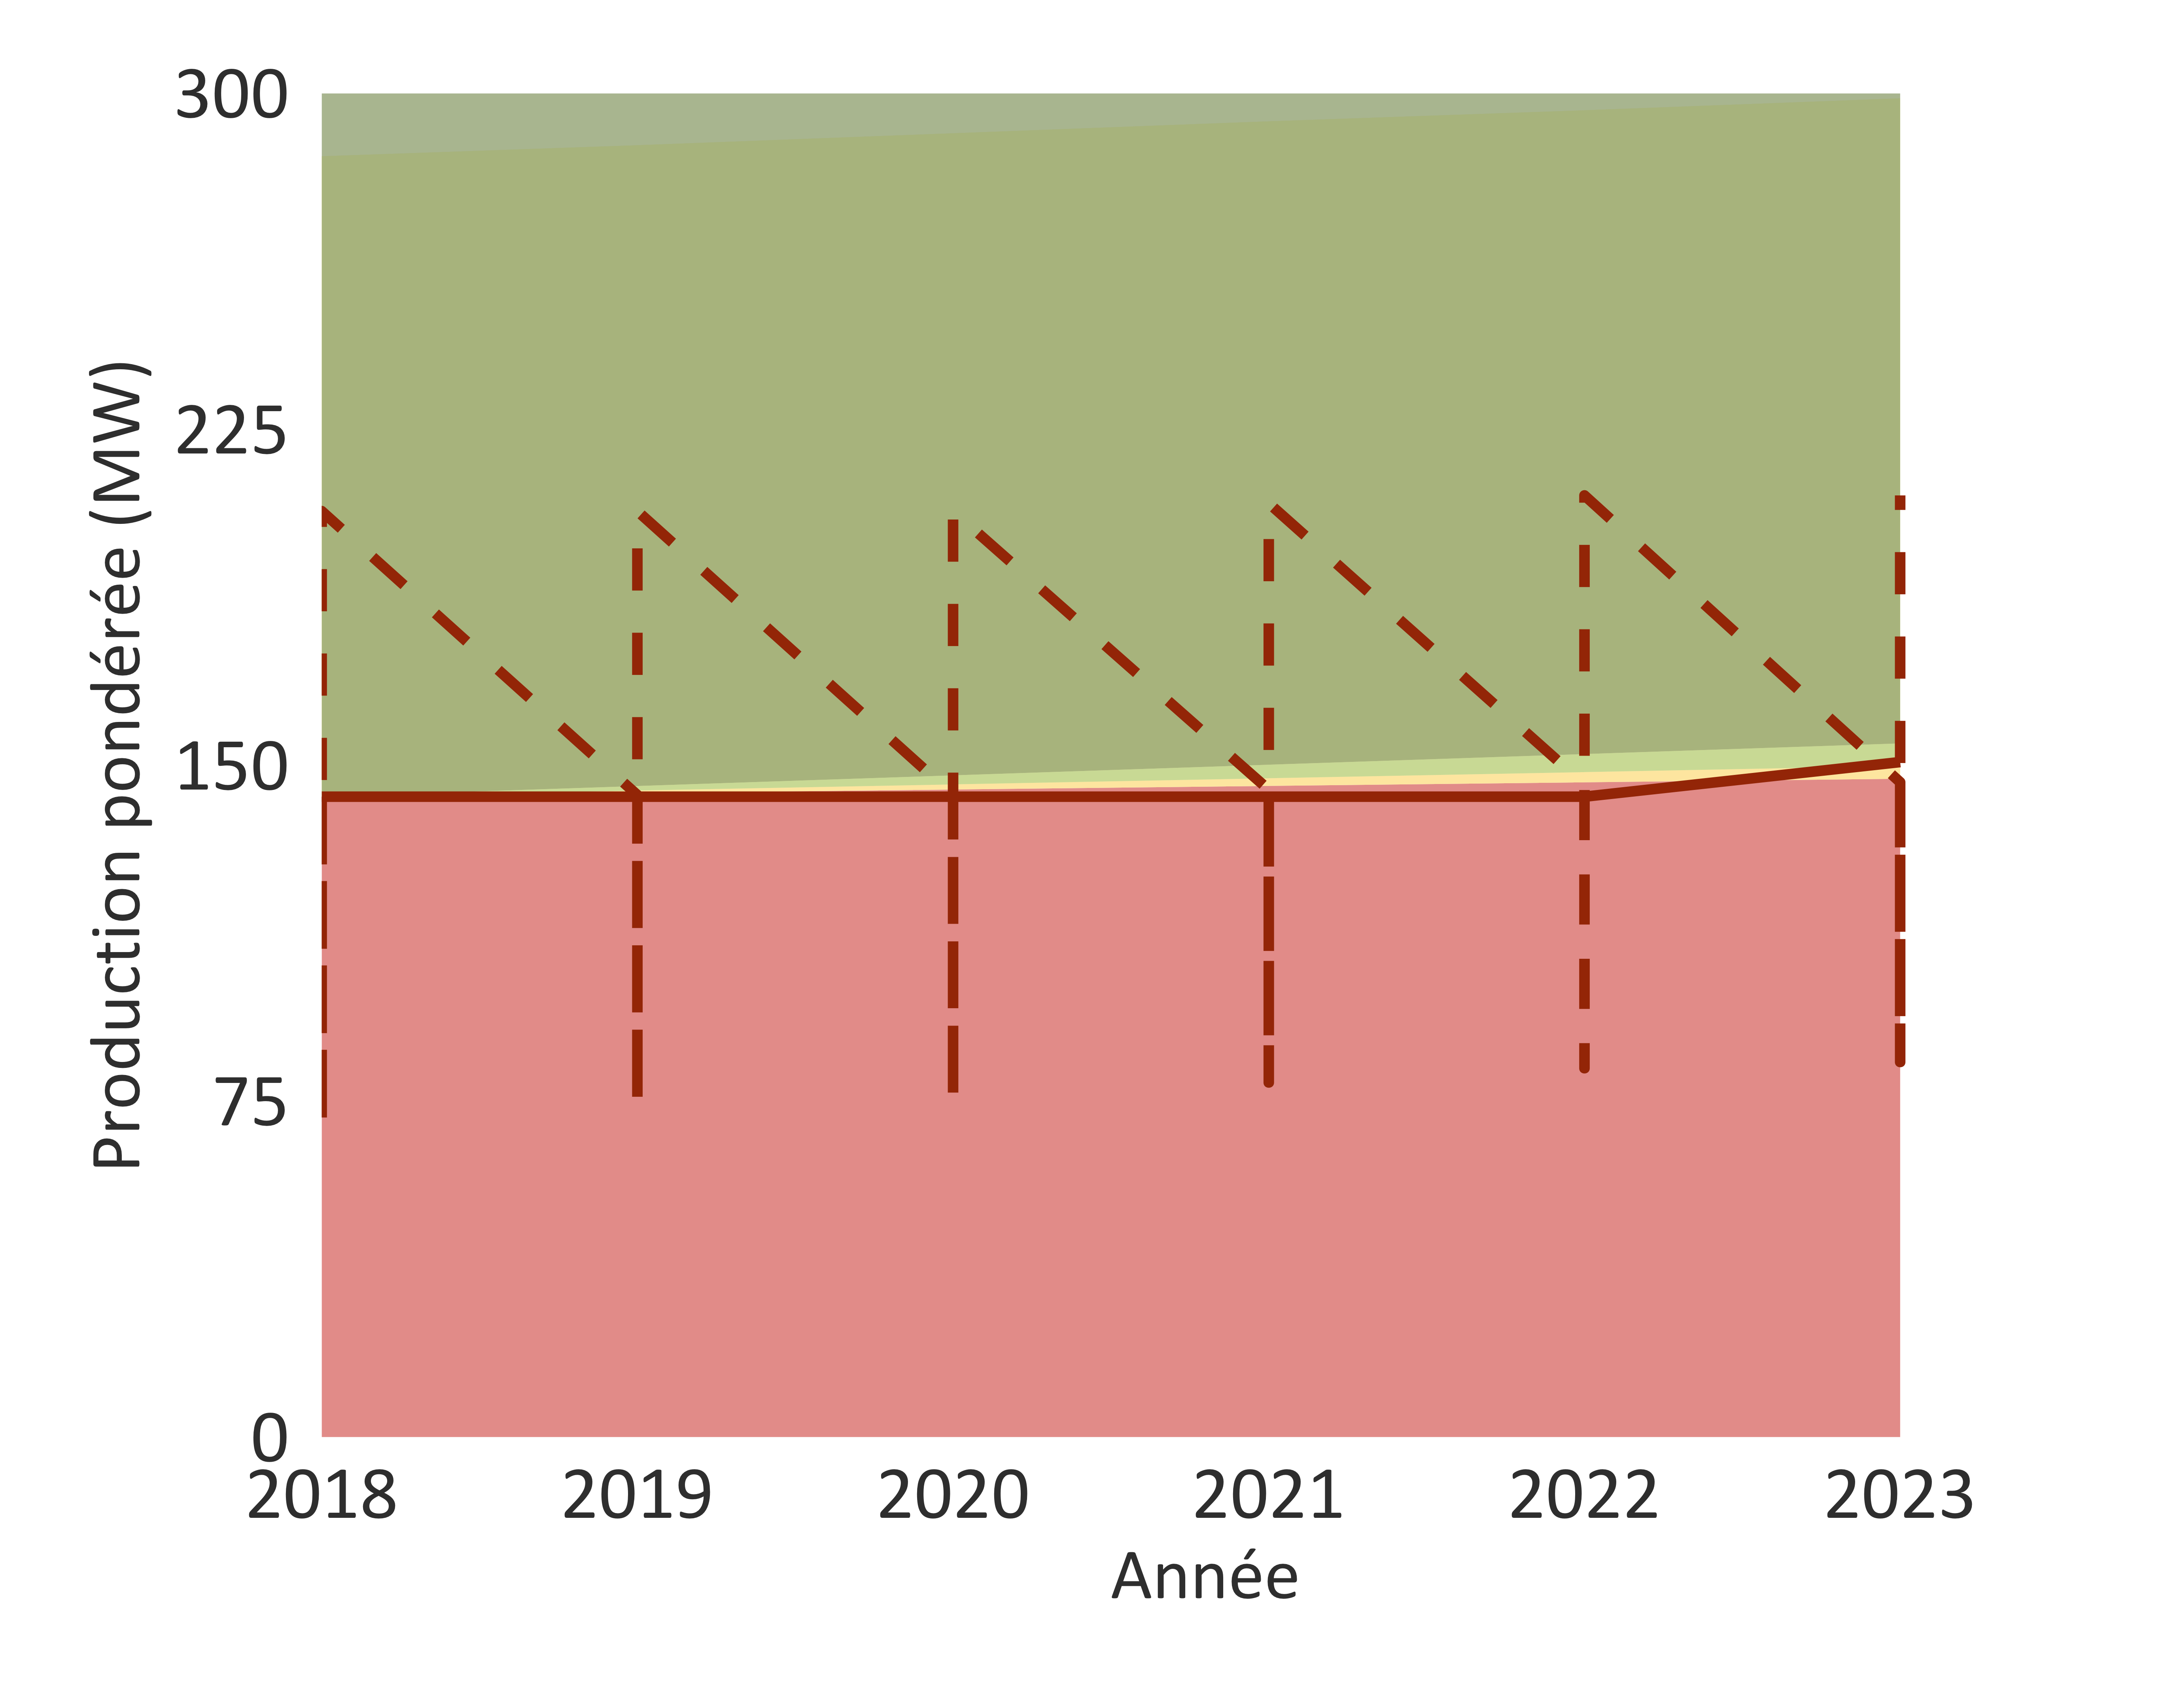
\includegraphics[trim = {0 0cm 0 0},width=1\linewidth]{ReportOutputs/Fig20}
		%WWFSpecificExcludeE
		
	\end{minipage}
	
	\vspace{-0.6cm}
	\begin{center}
		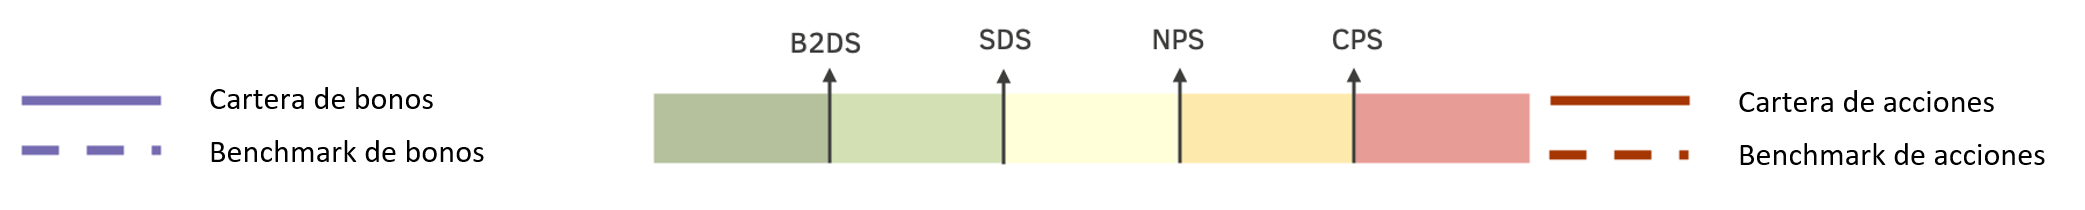
\includegraphics[trim = {0 0cm 0 0},width=.9\linewidth]{ReportGraphics/246Legend_ES.png}
	\end{center}

	\small\textit{*Debido a diferentes supuestos en los escenarios B2DS y SDS sobre la  combinación tecnológica esperada en el sector de energías renovables, el escenario SDS puede parecer más ambicioso que el B2DS. Sin embargo, en el escenario B2DS se espera que la generación de energía renovable sea mayor a la del SDS a pesar de que la capacidad sea menor.}
	
	
	%\PageFooterThird
\PageFooter{3 - TRAYECTORIA DE LA CARTERA}
	\newpage 
	%PowerSector_EQE
	%PowerSector_ALLE

	%FossilFuelSector_ALLS
	%FossilFuelSector_CBS
	\section*{} % TRAJECTORY - DEBT - FOSSIL FUELS AND AUTOMOTIVE   
	\HeaderDouble{TENDENCIA DE 5 AÑOS – BONOS CORPORATIVOS}{SECTOR DE COMBUSTIBLES FÓSILES}	
	
	\begin{multicols}{2}
		\textbf{Los gráficos de alineación a continuación muestran la alineación de tecnologías en el sector de combustibles fósiles de la cartera de bonos corporativos respecto a los escenarios de transición de la AIE: B2DS, SDS, NPS, CPS y la alineación del mercado de bonos.} 
		Para cada tecnología, el valor graficado de la cartera (línea continua) representa la evolución planeada o “trayectoria” de producción de combustibles fósiles atribuida a la cartera de bonos corporativos en los próximos 5 años.      
		Las líneas que separan las áreas del fondo codificado por colores representan la “producción objetivo” de la cartera para cada tecnología bajo los escenarios de la AIE. La línea punteada representa la producción planeada por tecnología en el mercado de bonos, ajustada al mismo punto de inicio de la cartera.            
		
		
	\end{multicols}		
	

	\begin{minipage}[t]{.49\linewidth}
		\textbf{Trayectoria de Producción de Petróleo}
		
		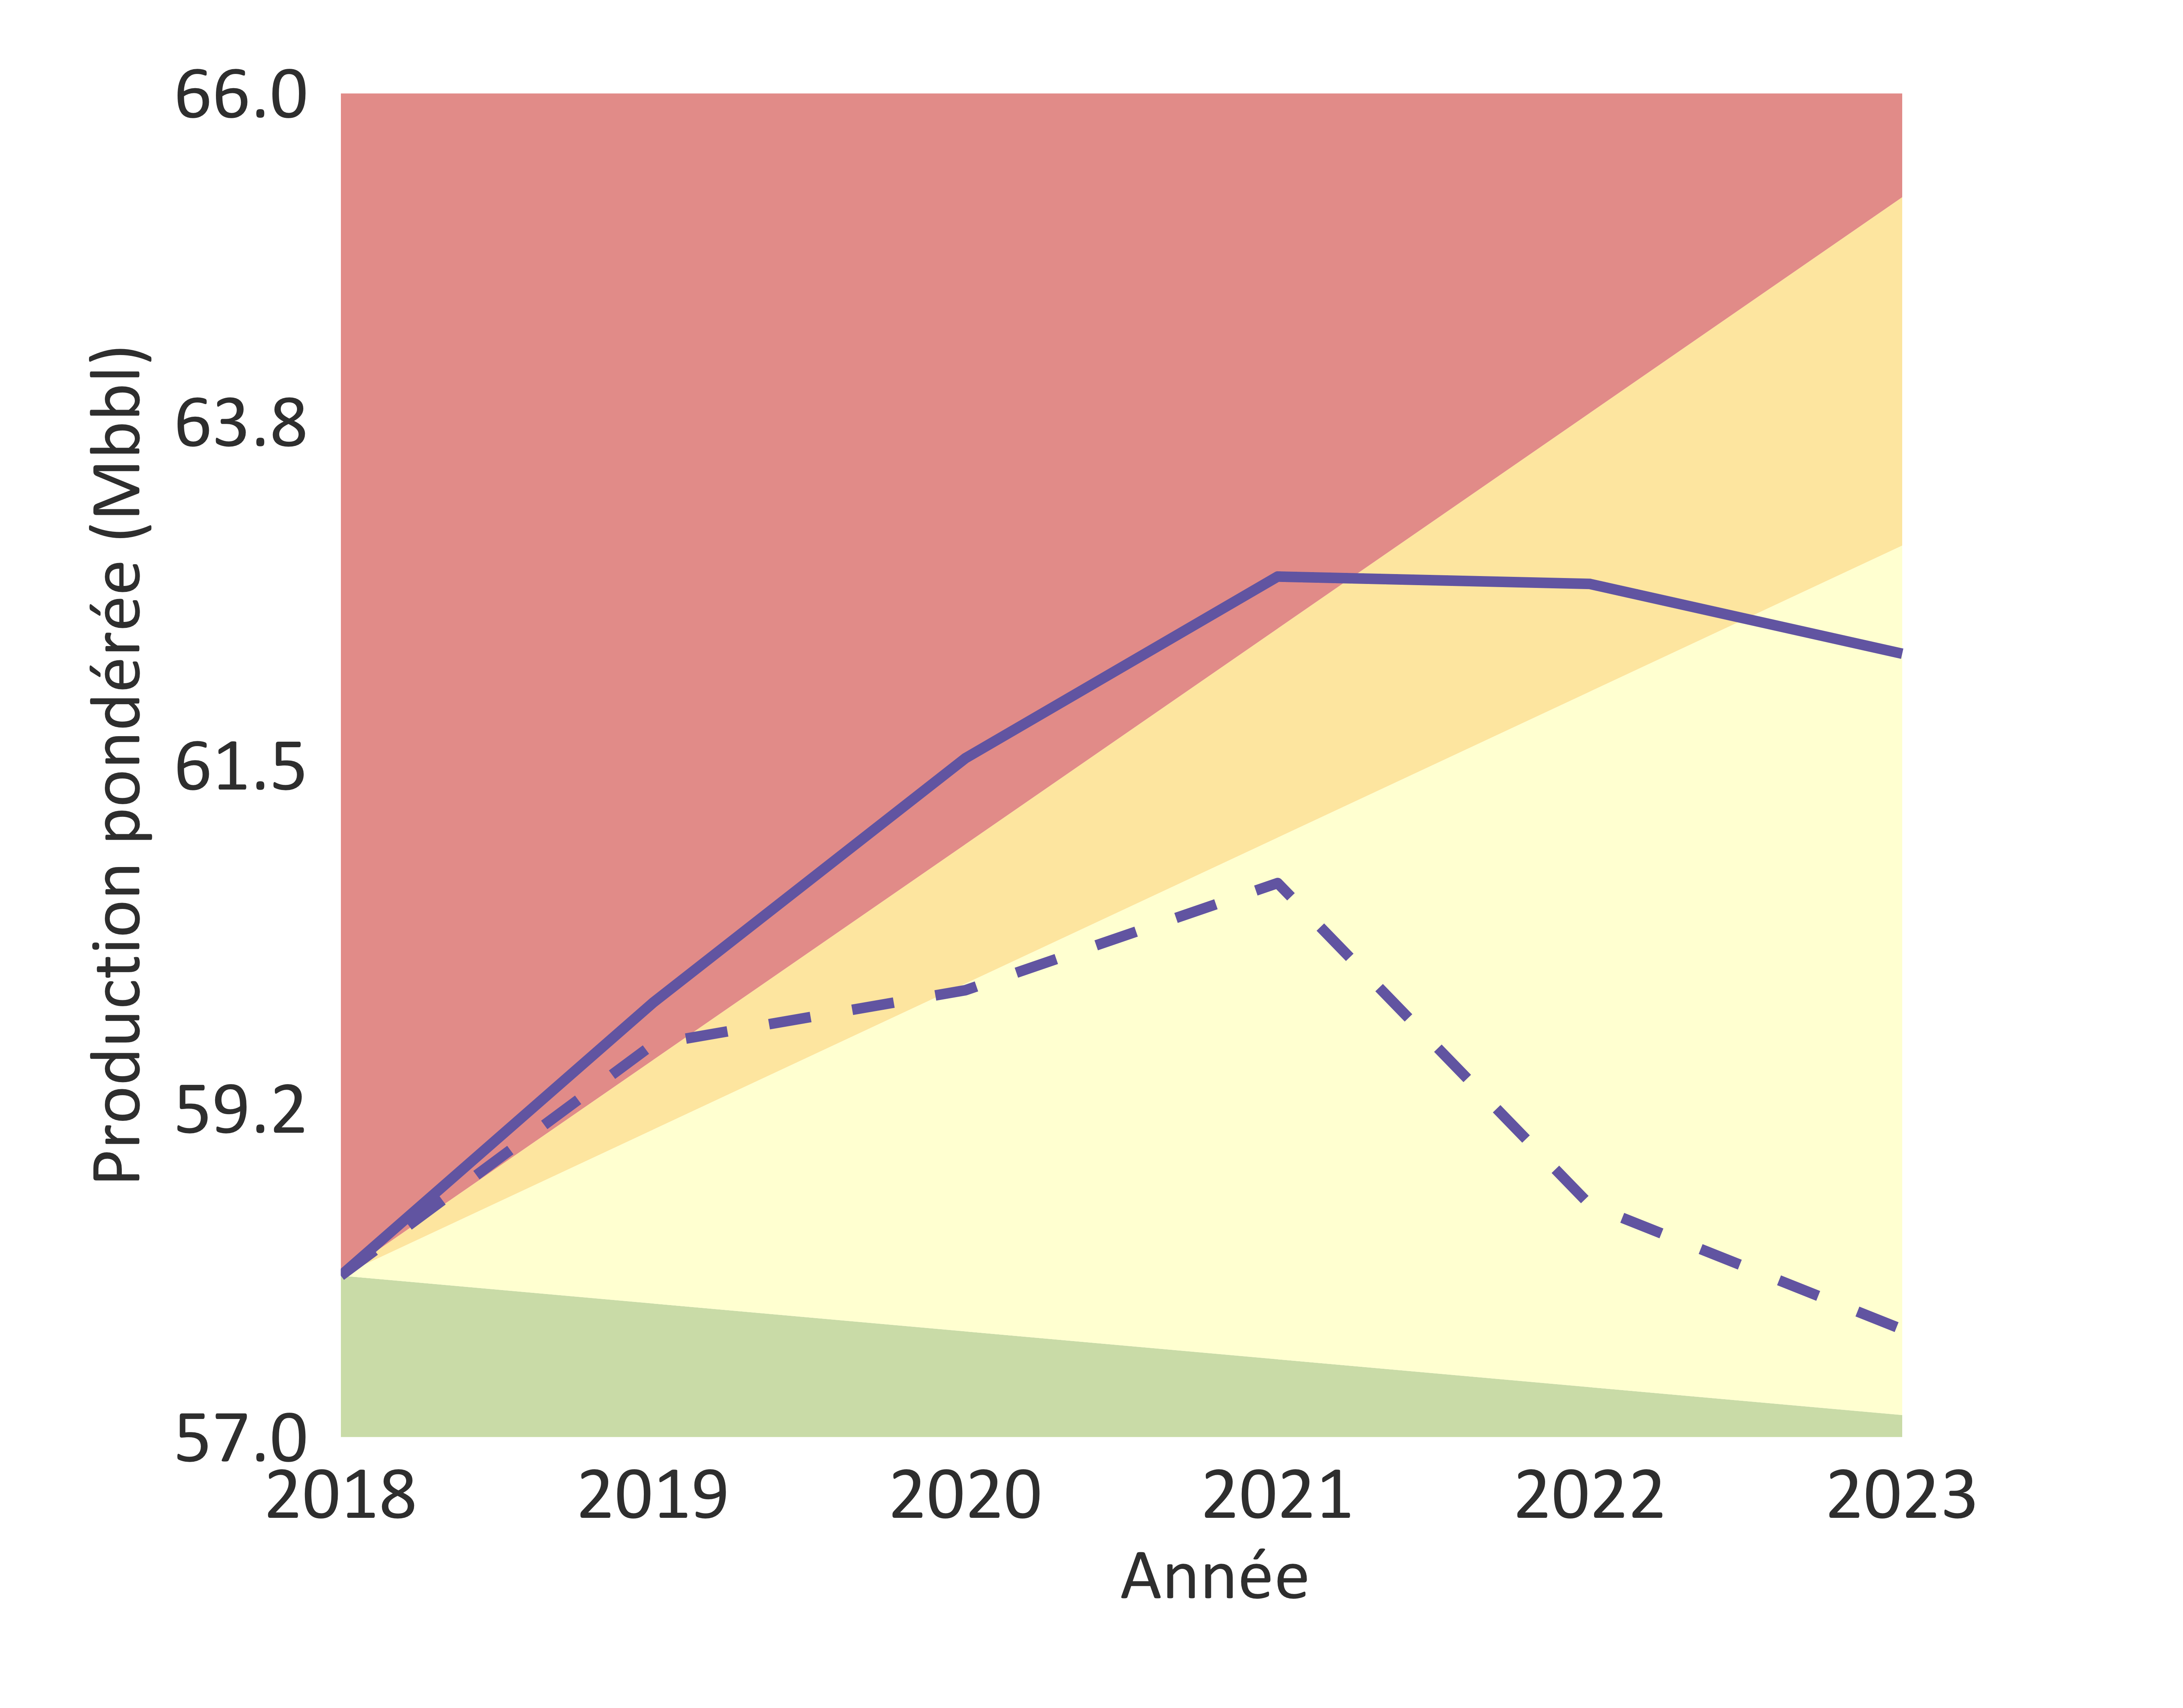
\includegraphics[trim = {0 0cm 0 0},width=1\linewidth]{ReportOutputs/Fig11}
		
	\end{minipage}	
	\hspace{.02\linewidth}
	\begin{minipage}[t]{.49\textwidth}
		\textbf{Trayectoria de Producción de Gas }
		
		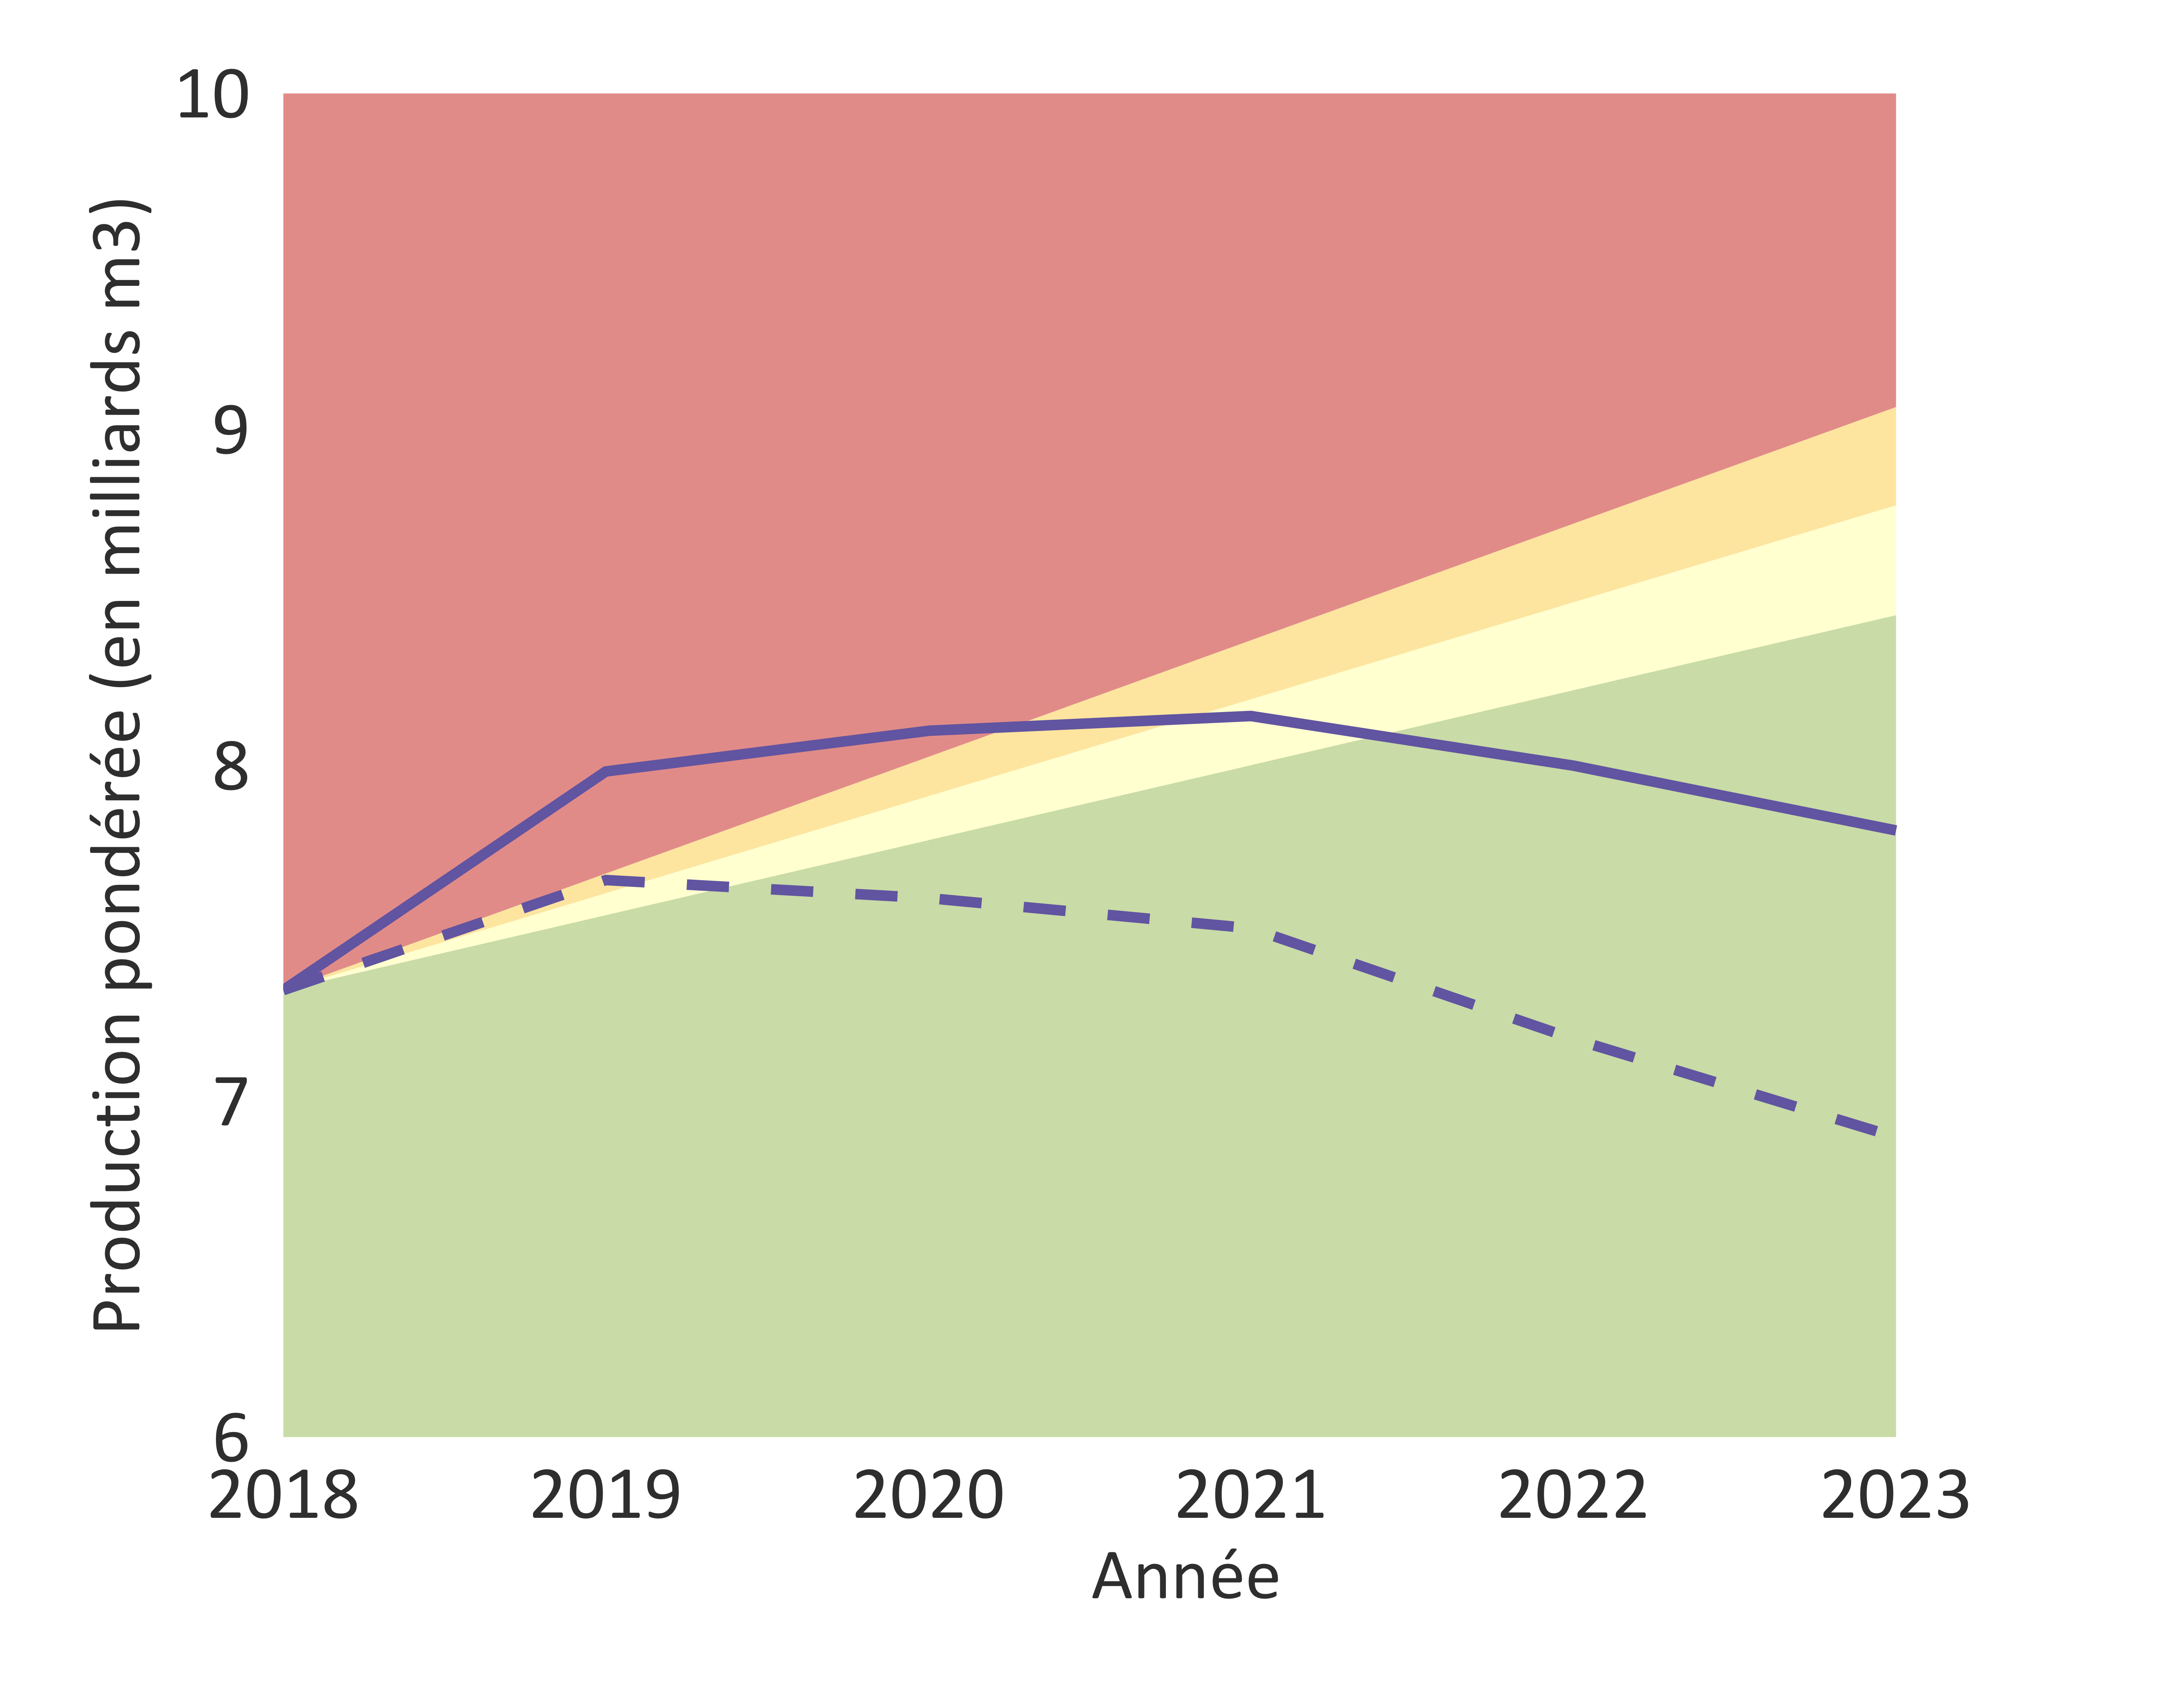
\includegraphics[trim = {0 0cm 0 0},width=1\linewidth]{ReportOutputs/Fig12}
		
	\end{minipage}
	
	

	\begin{minipage}[t]{.49\linewidth}
		\textbf{Trayectoria de Producción de Carbón}
		
		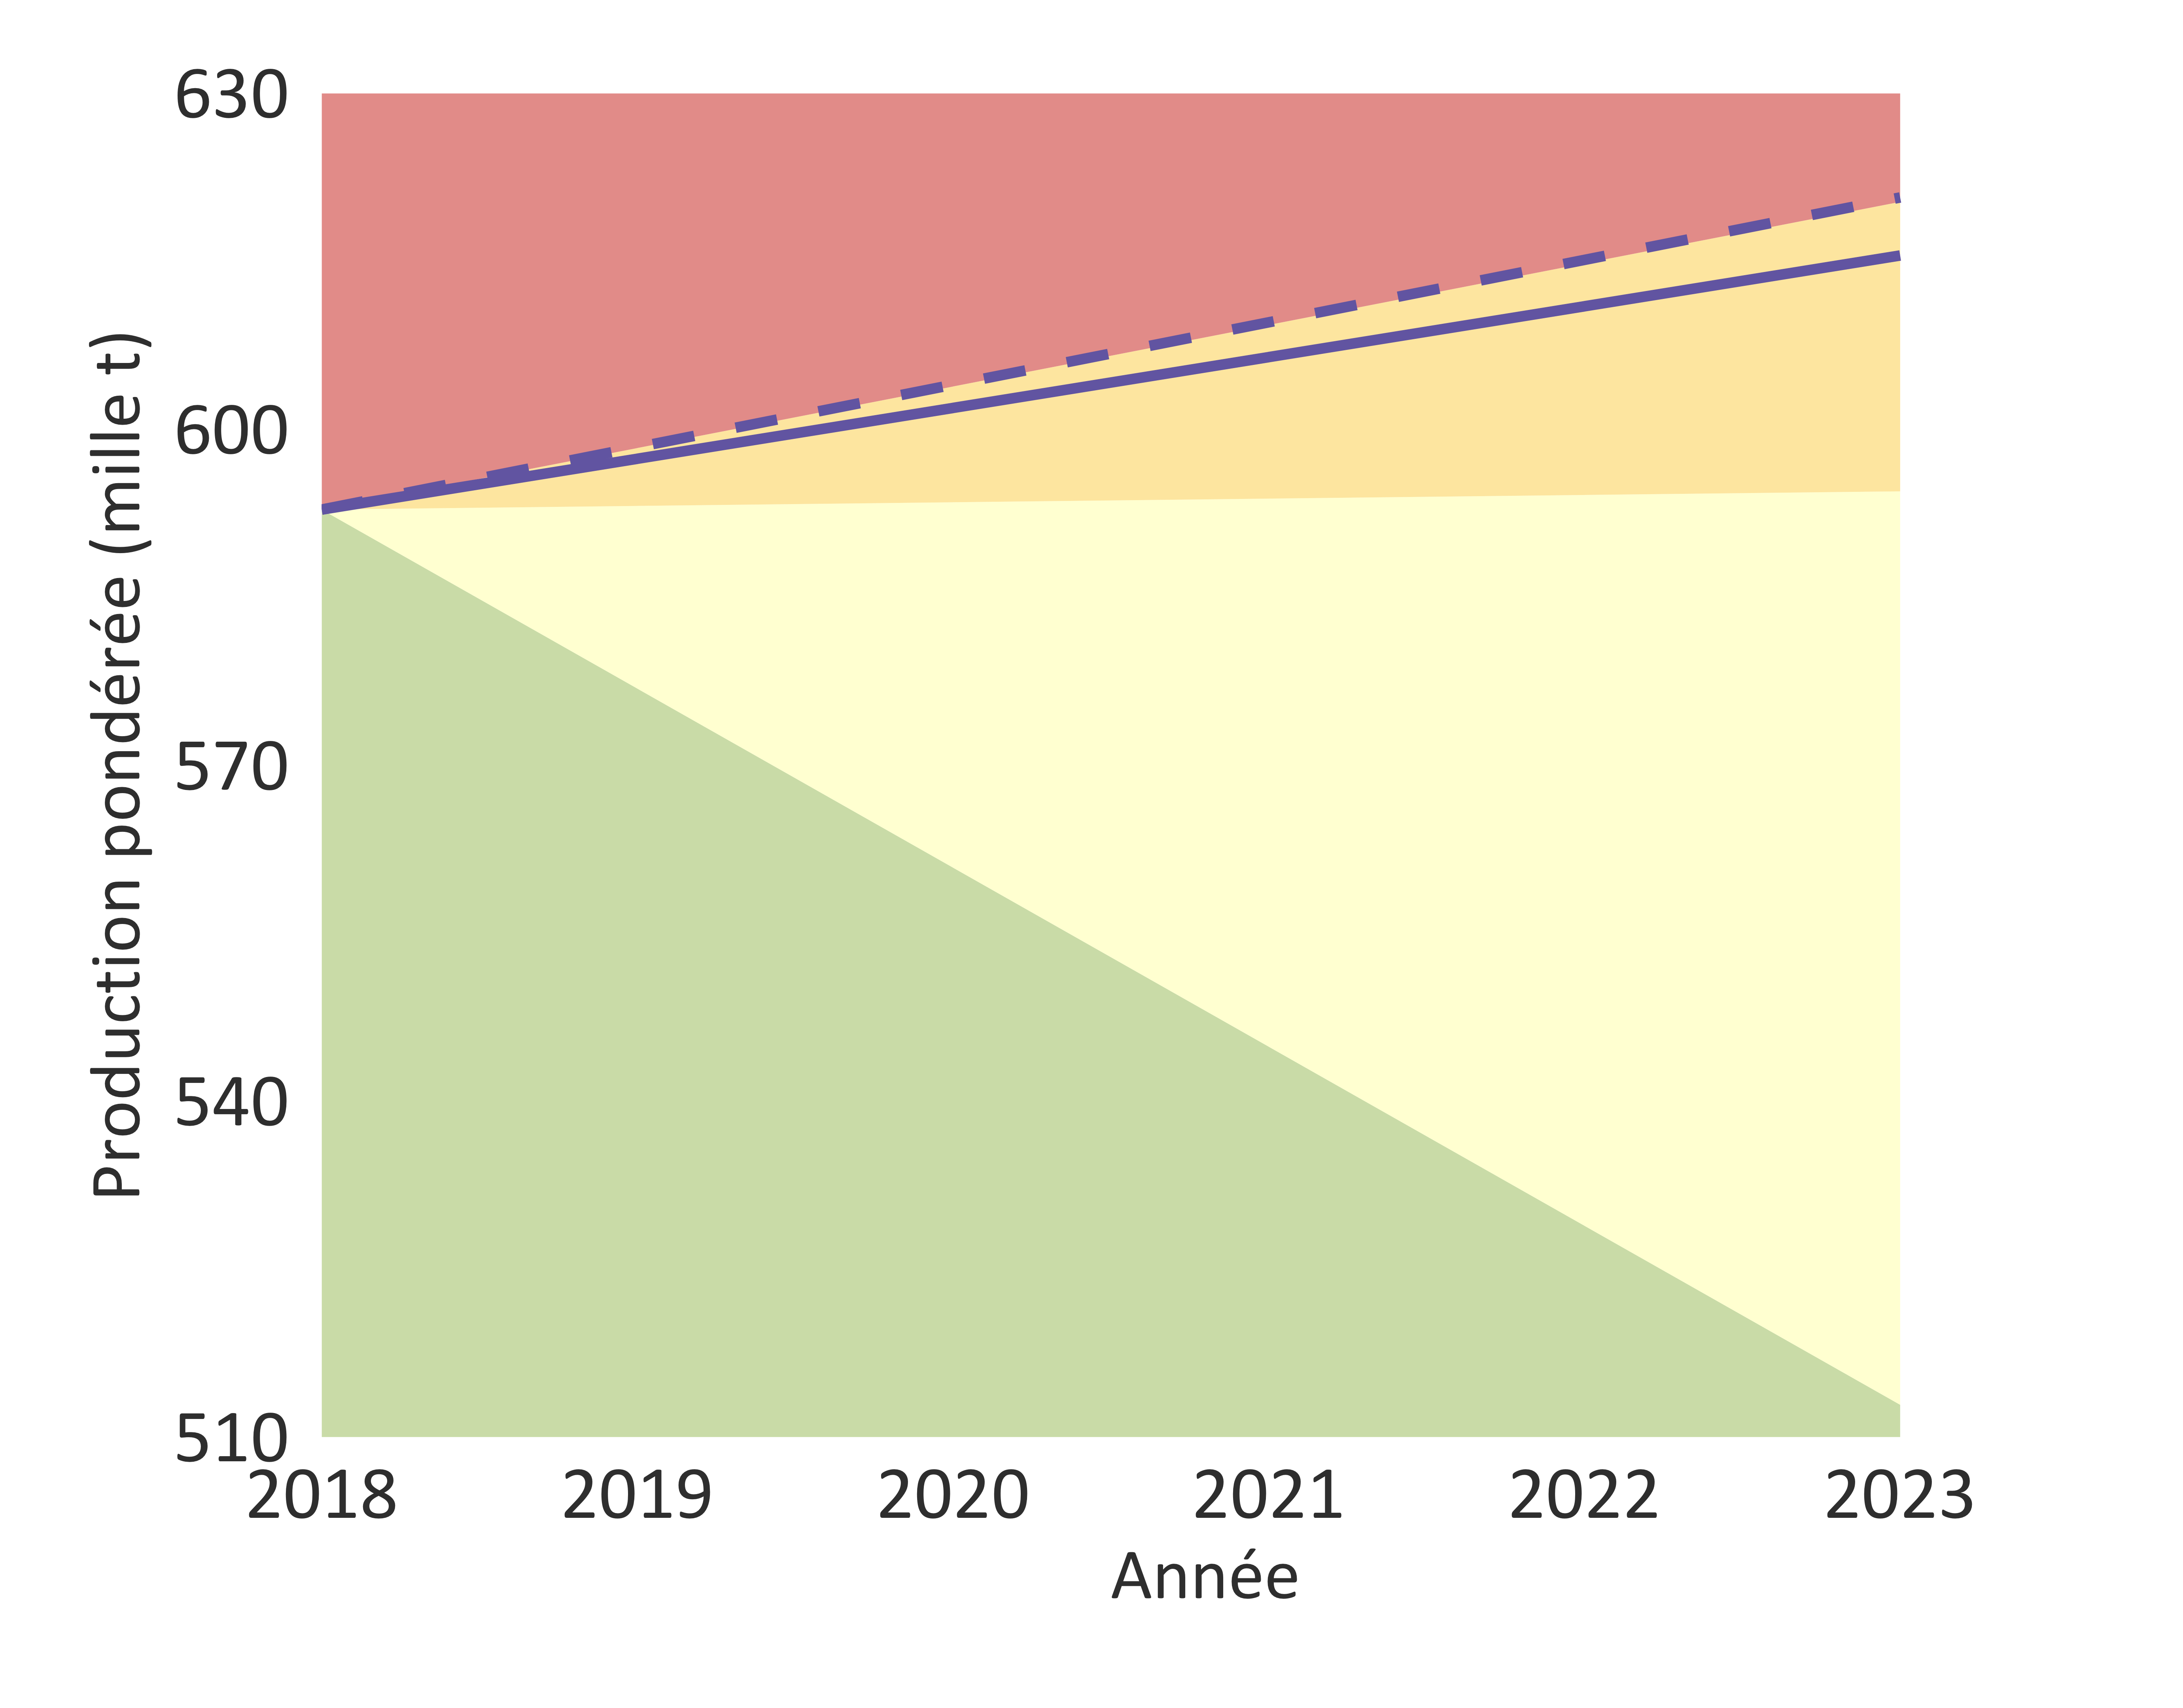
\includegraphics[trim = {0 0cm 0 0},width=1\linewidth]{ReportOutputs/Fig13}
		
	\end{minipage}	
		
	
	\vspace{-.6cm}
	\begin{center}
		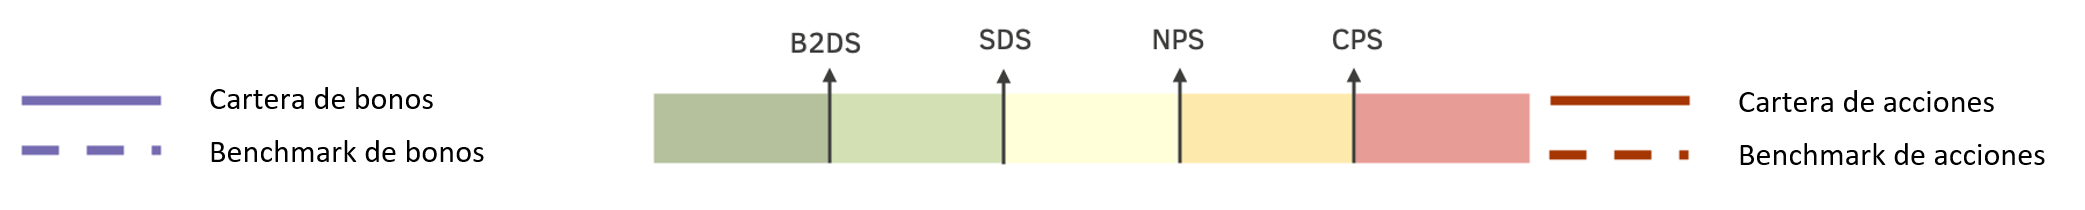
\includegraphics[trim = {0 0cm 0 0},width=.9\linewidth]{ReportGraphics/246Legend_ES.png}
	\end{center}

	
	%\PageFooterThird
\PageFooter{3 - TRAYECTORIA DE LA CARTERA}

	\newpage 
	%FossilFuelSector_CBE
	%FossilFuelSector_EQS 
	\section*{} % TRAJECTORY - EQUITY - FOSSIL FUELS AND AUTOMOTIVE  
	\HeaderDouble{TENDENCIA A 5 AÑOS – ACCIONES}{SECTOR DE COMBUSTIBLES FÓSILES}	
	
	\begin{multicols}{2}
		\textbf{Los gráficos de alineación a continuación muestran la alineación de tecnologías en el sector de combustibles fósiles de la cartera de acciones respecto a los escenarios de transición de la AIE: B2DS, SDS, NPS, CPS y la alineación del mercado de acciones.   } 
		Para cada tecnología, el valor graficado de la cartera (línea continua) representa la evolución estimada o “trayectoria” de producción de combustibles fósiles atribuida a la cartera de acciones en los próximos 5 años.                
		Las líneas que separan las áreas del fondo codificado por colores representan la “producción objetivo” de la cartera para cada tecnología bajo los escenarios de la AIE. La línea punteada representa la producción planeada por tecnología para el mercado de acciones, ajustada al mismo punto de inicio de la cartera.
		
		
	\end{multicols}		

	
	\begin{minipage}[t]{.49\linewidth}
		\textbf{Trayectoria de Producción de Petróleo }
		
		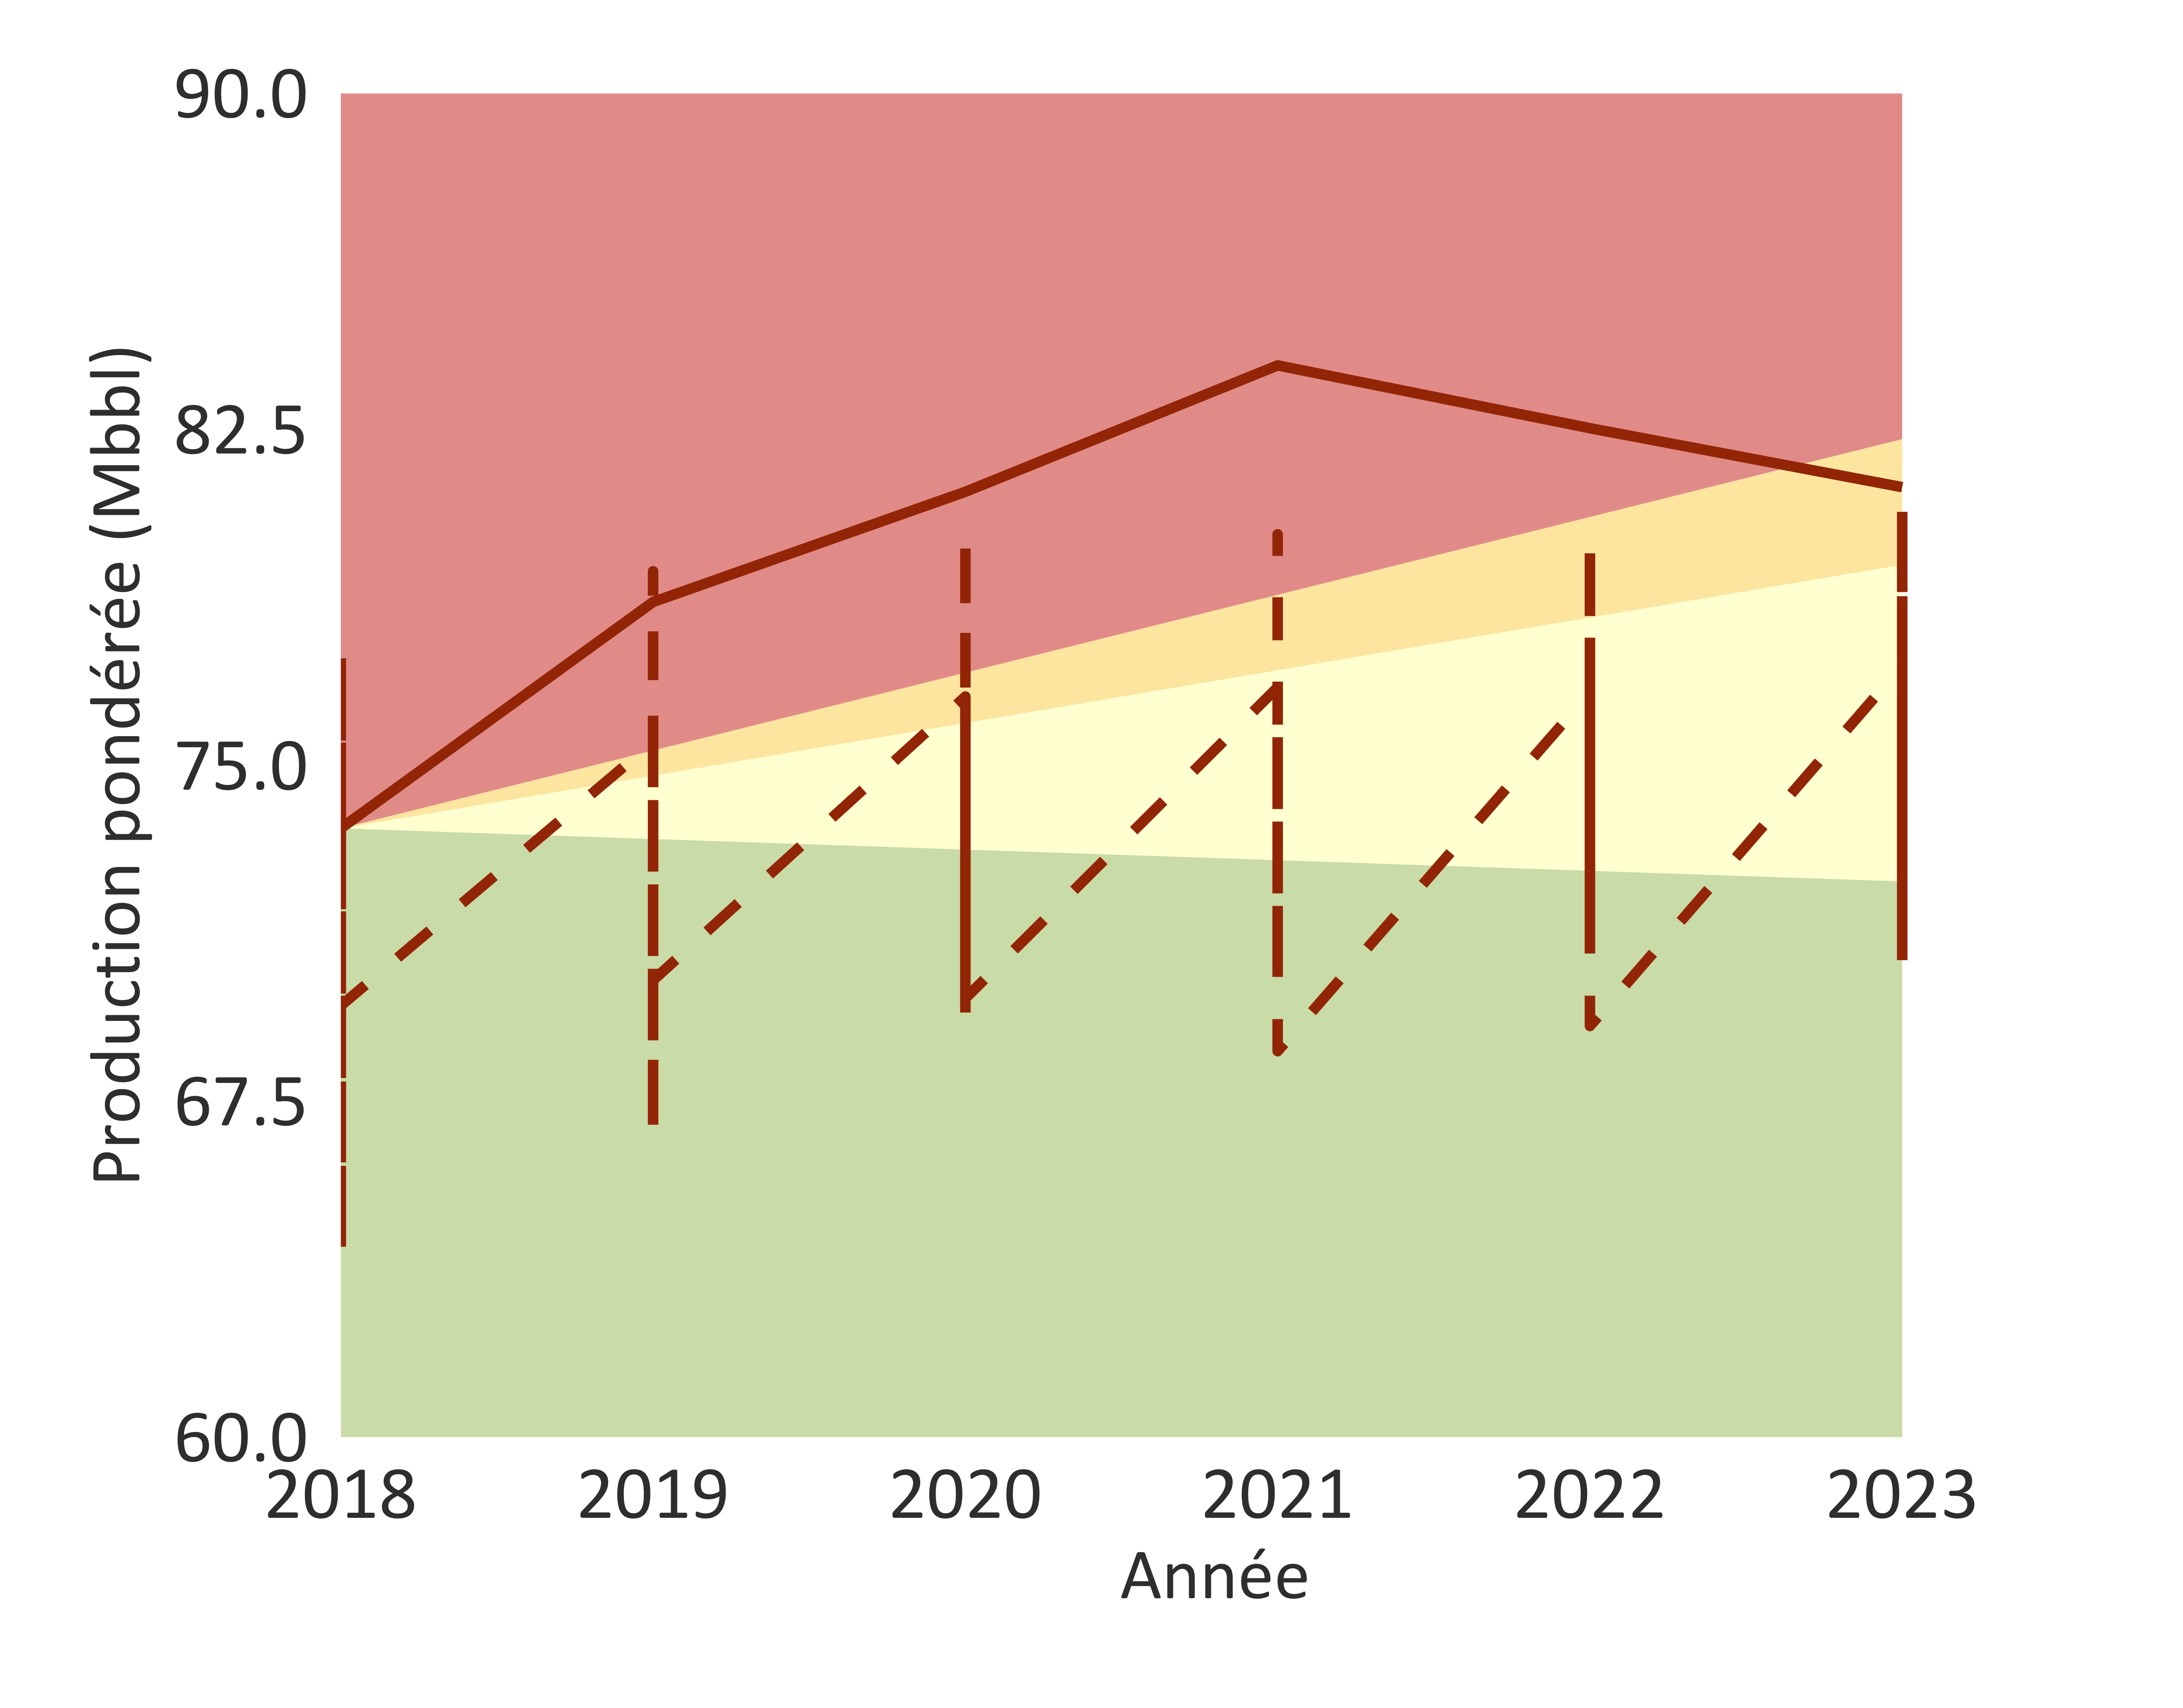
\includegraphics[trim = {0 0cm 0 0},width=1\linewidth]{ReportOutputs/Fig21}
		
	\end{minipage}	
	\hspace{.02\linewidth}
	\begin{minipage}[t]{.49\textwidth}
		\textbf{Trayectoria de Producción de Gas}
		
		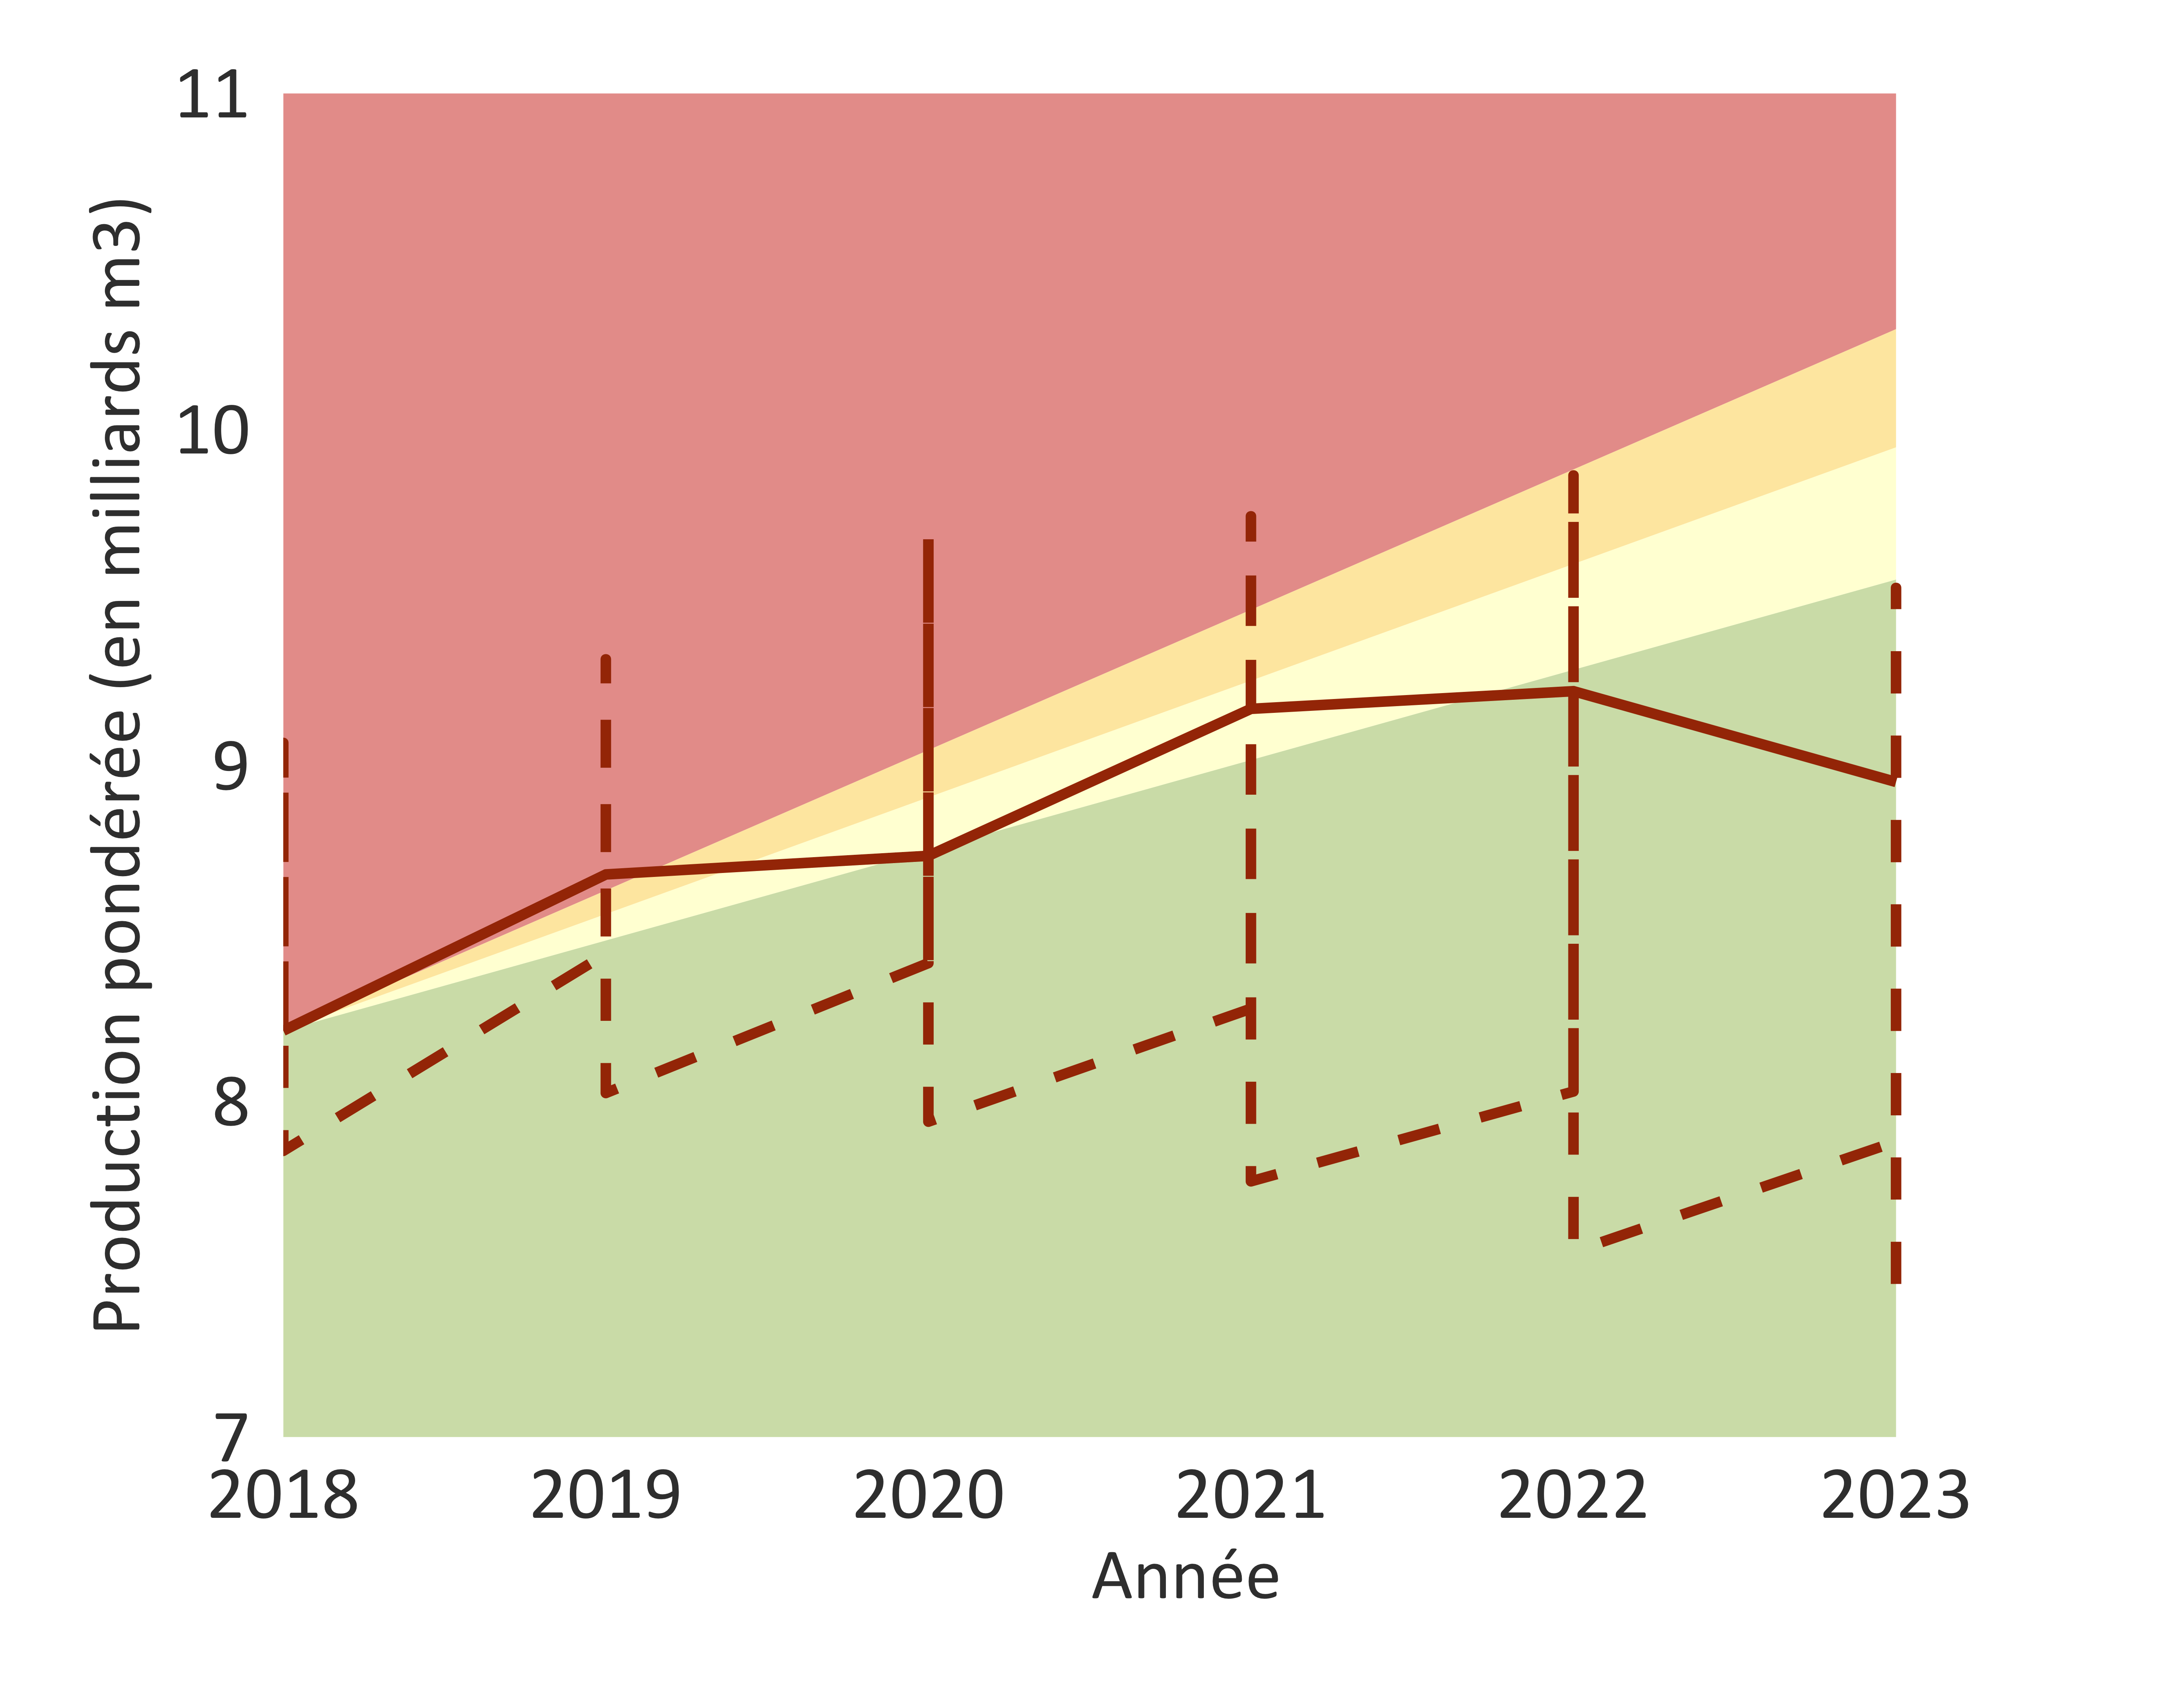
\includegraphics[trim = {0 0cm 0 0},width=1\linewidth]{ReportOutputs/Fig22}
		
	\end{minipage}
	
	
	
	\begin{minipage}[t]{.49\linewidth}
		\textbf{Trayectoria de Producción de Carbón}
		
		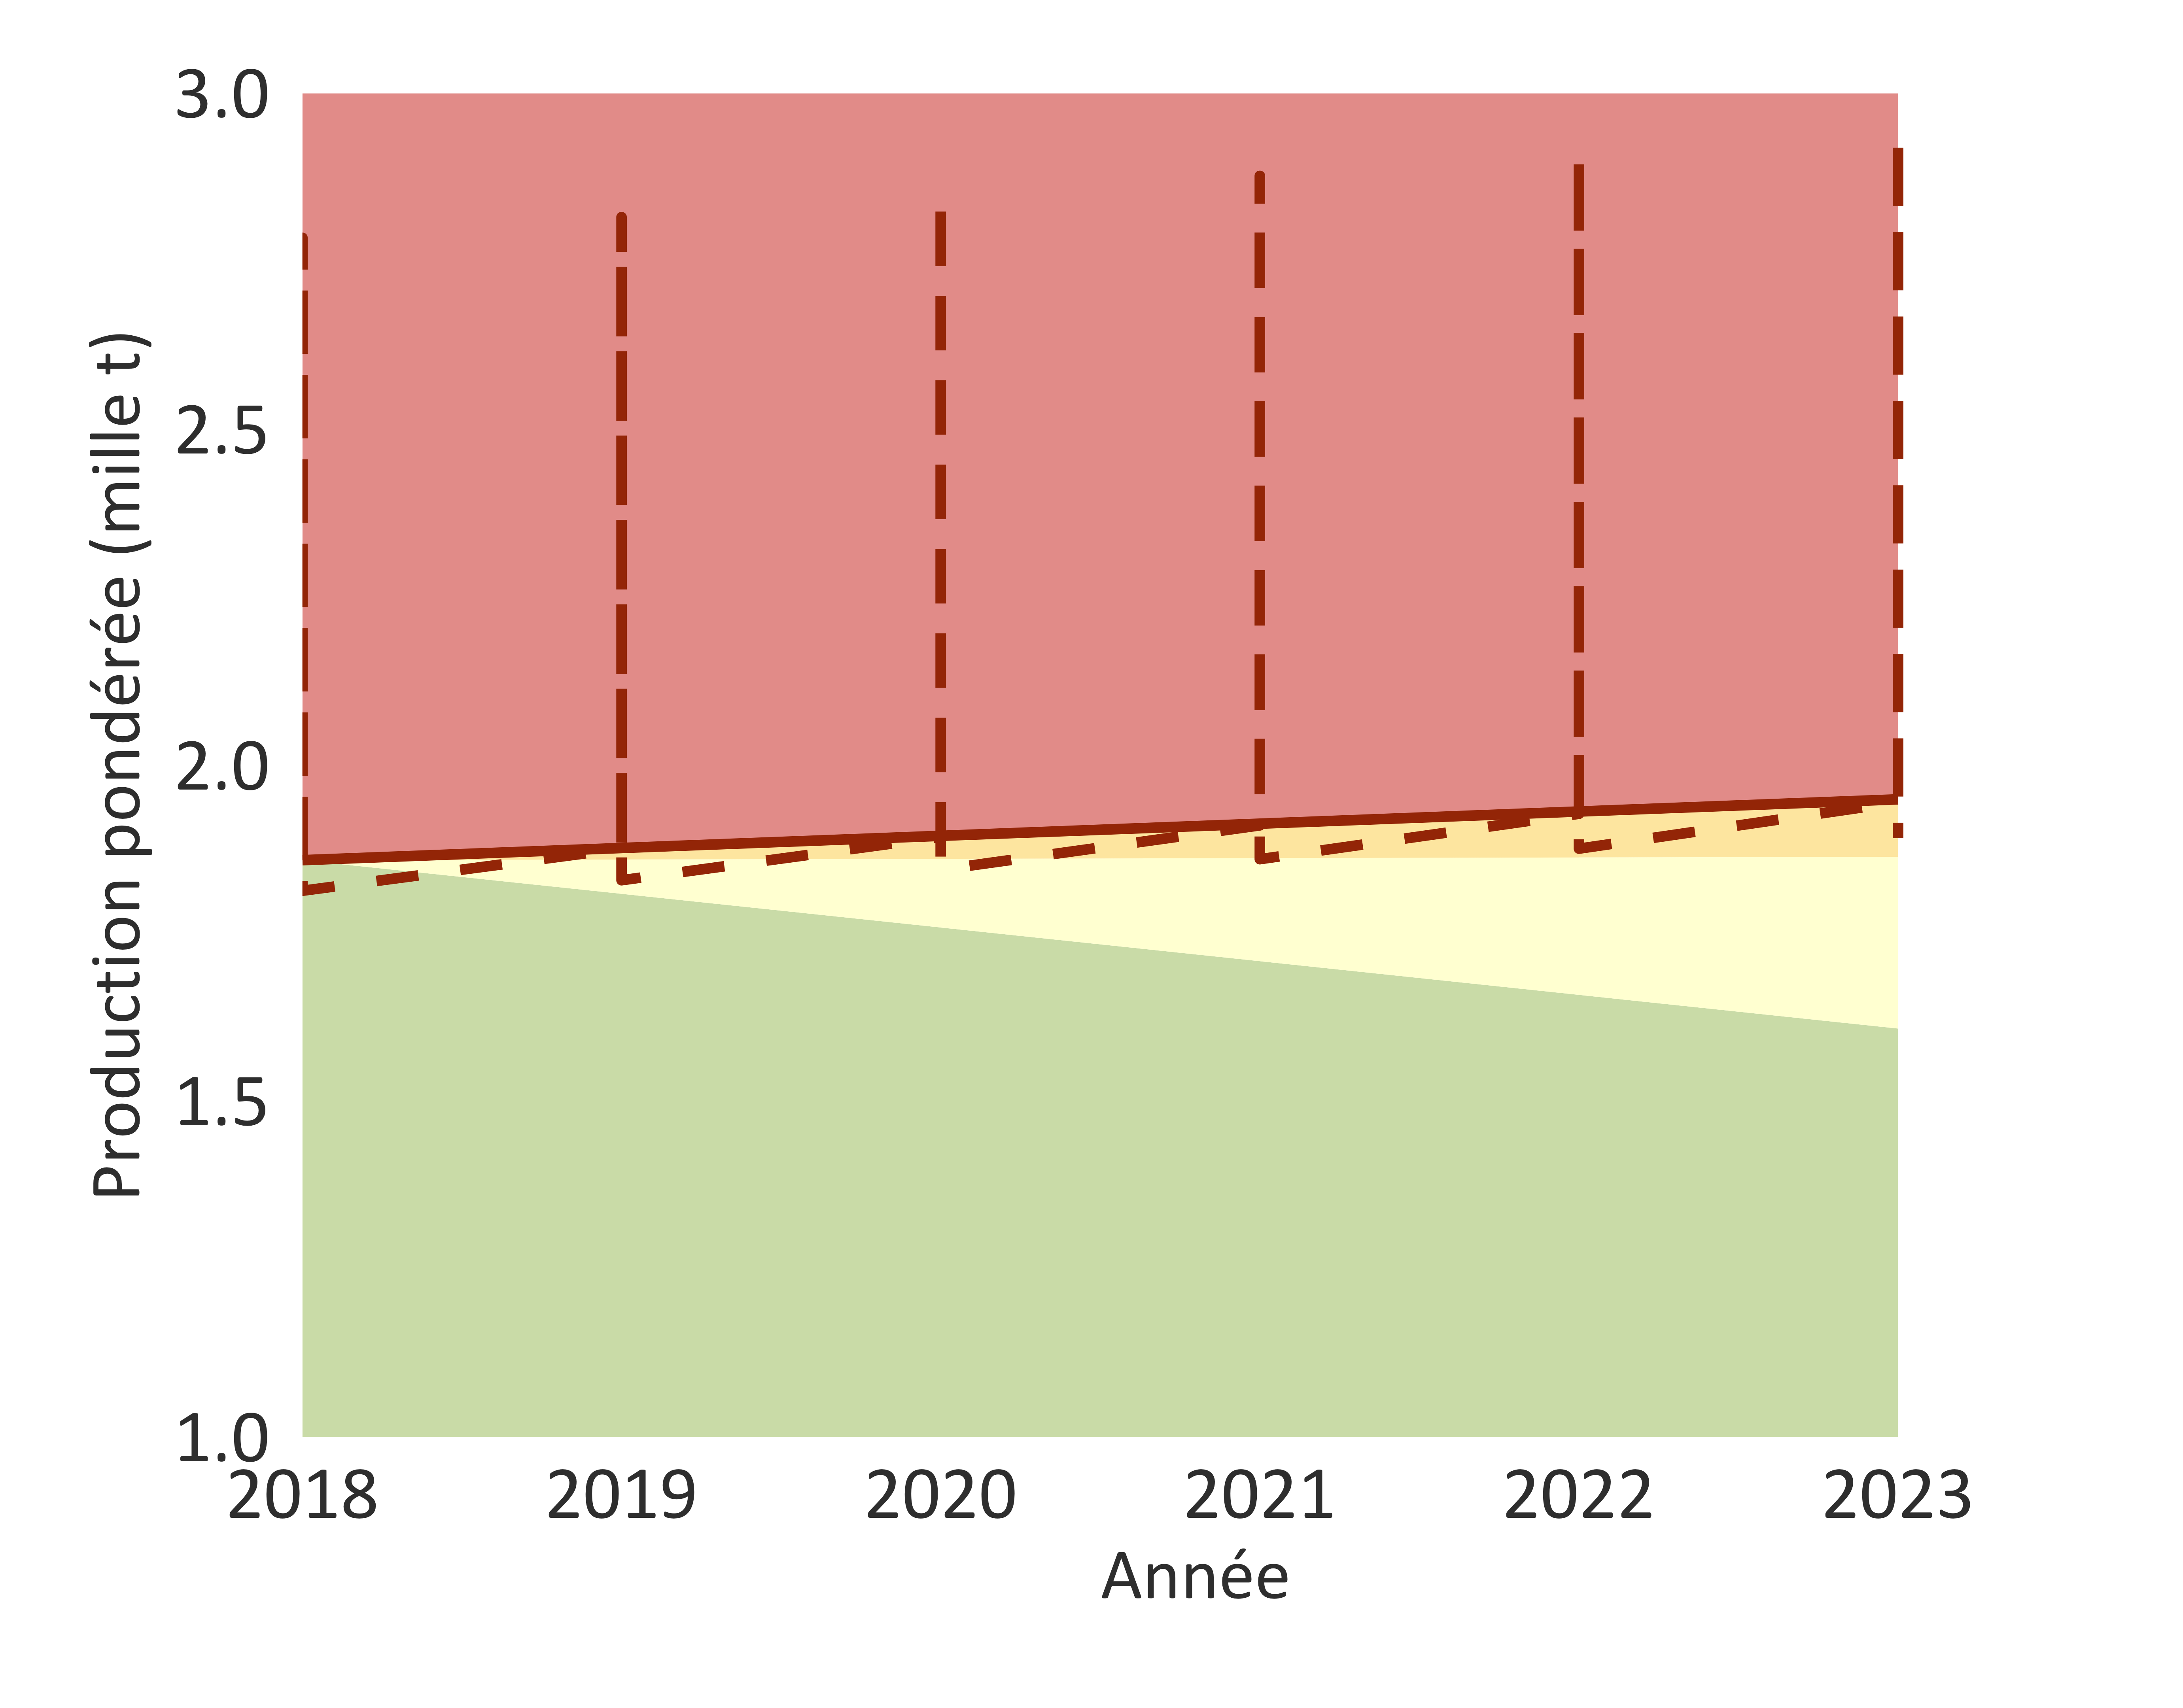
\includegraphics[trim = {0 0cm 0 0},width=1\linewidth]{ReportOutputs/Fig23}
		
	\end{minipage}	
	
	
	\vspace{-.6cm}
	\begin{center}
		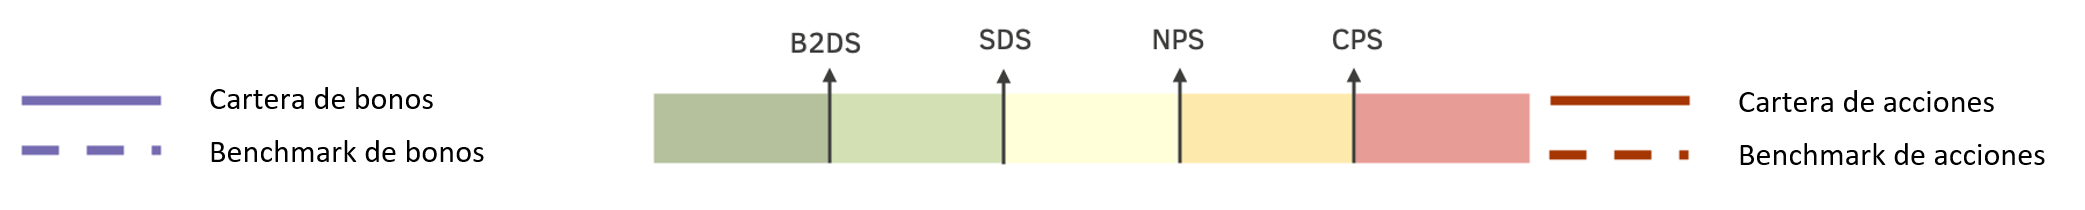
\includegraphics[trim = {0 0cm 0 0},width=.9\linewidth]{ReportGraphics/246Legend_ES.png}
	\end{center}
	
	
	%\PageFooterThird
\PageFooter{3 - TRAYECTORIA DE LA CARTERA}
	
	\newpage  
	%FossilFuelSector_EQE 
	%FossilFuelSector_ALLE
	%AutoSector_ALLS
	%AutoSector_CBS
	\section*{} % TRAJECTORY - BONDS - AUTOMOTIVE  
	\HeaderDouble{TENDENCIA A 5 AÑOS – BONOS CORPORATIVOS}{SECTOR AUTOMOTRIZ}	
	
	\begin{multicols}{2}
		\textbf{Los gráficos de alineación a continuación muestran la alineación de tecnologías automotrices en la cartera de bonos corporativos respecto a los escenarios de transición de la AIE: B2DS, SDS, NPS, CPS y la alineación del mercado de bonos.  } 
		Para cada tecnología, el valor graficado de la cartera (línea continua) representa la evolución estimada o “trayectoria” de la producción automotriz atribuida a la cartera de bonos corporativos en los próximos 5 años.                   
		Las líneas que separan las áreas del fondo codificado por colores representan la “producción objetivo” de la cartera para cada tecnología bajo los escenarios de la AIE. La línea punteada representa la trayectoria planeada por tecnología en el mercado de bonos, ajustada al mismo punto de inicio de la cartera.
		
	\end{multicols}		

	
	\begin{minipage}[t]{.49\linewidth}
		\textbf{Trayectoria de Producción de Vehículos de Combustión Interna}
		
		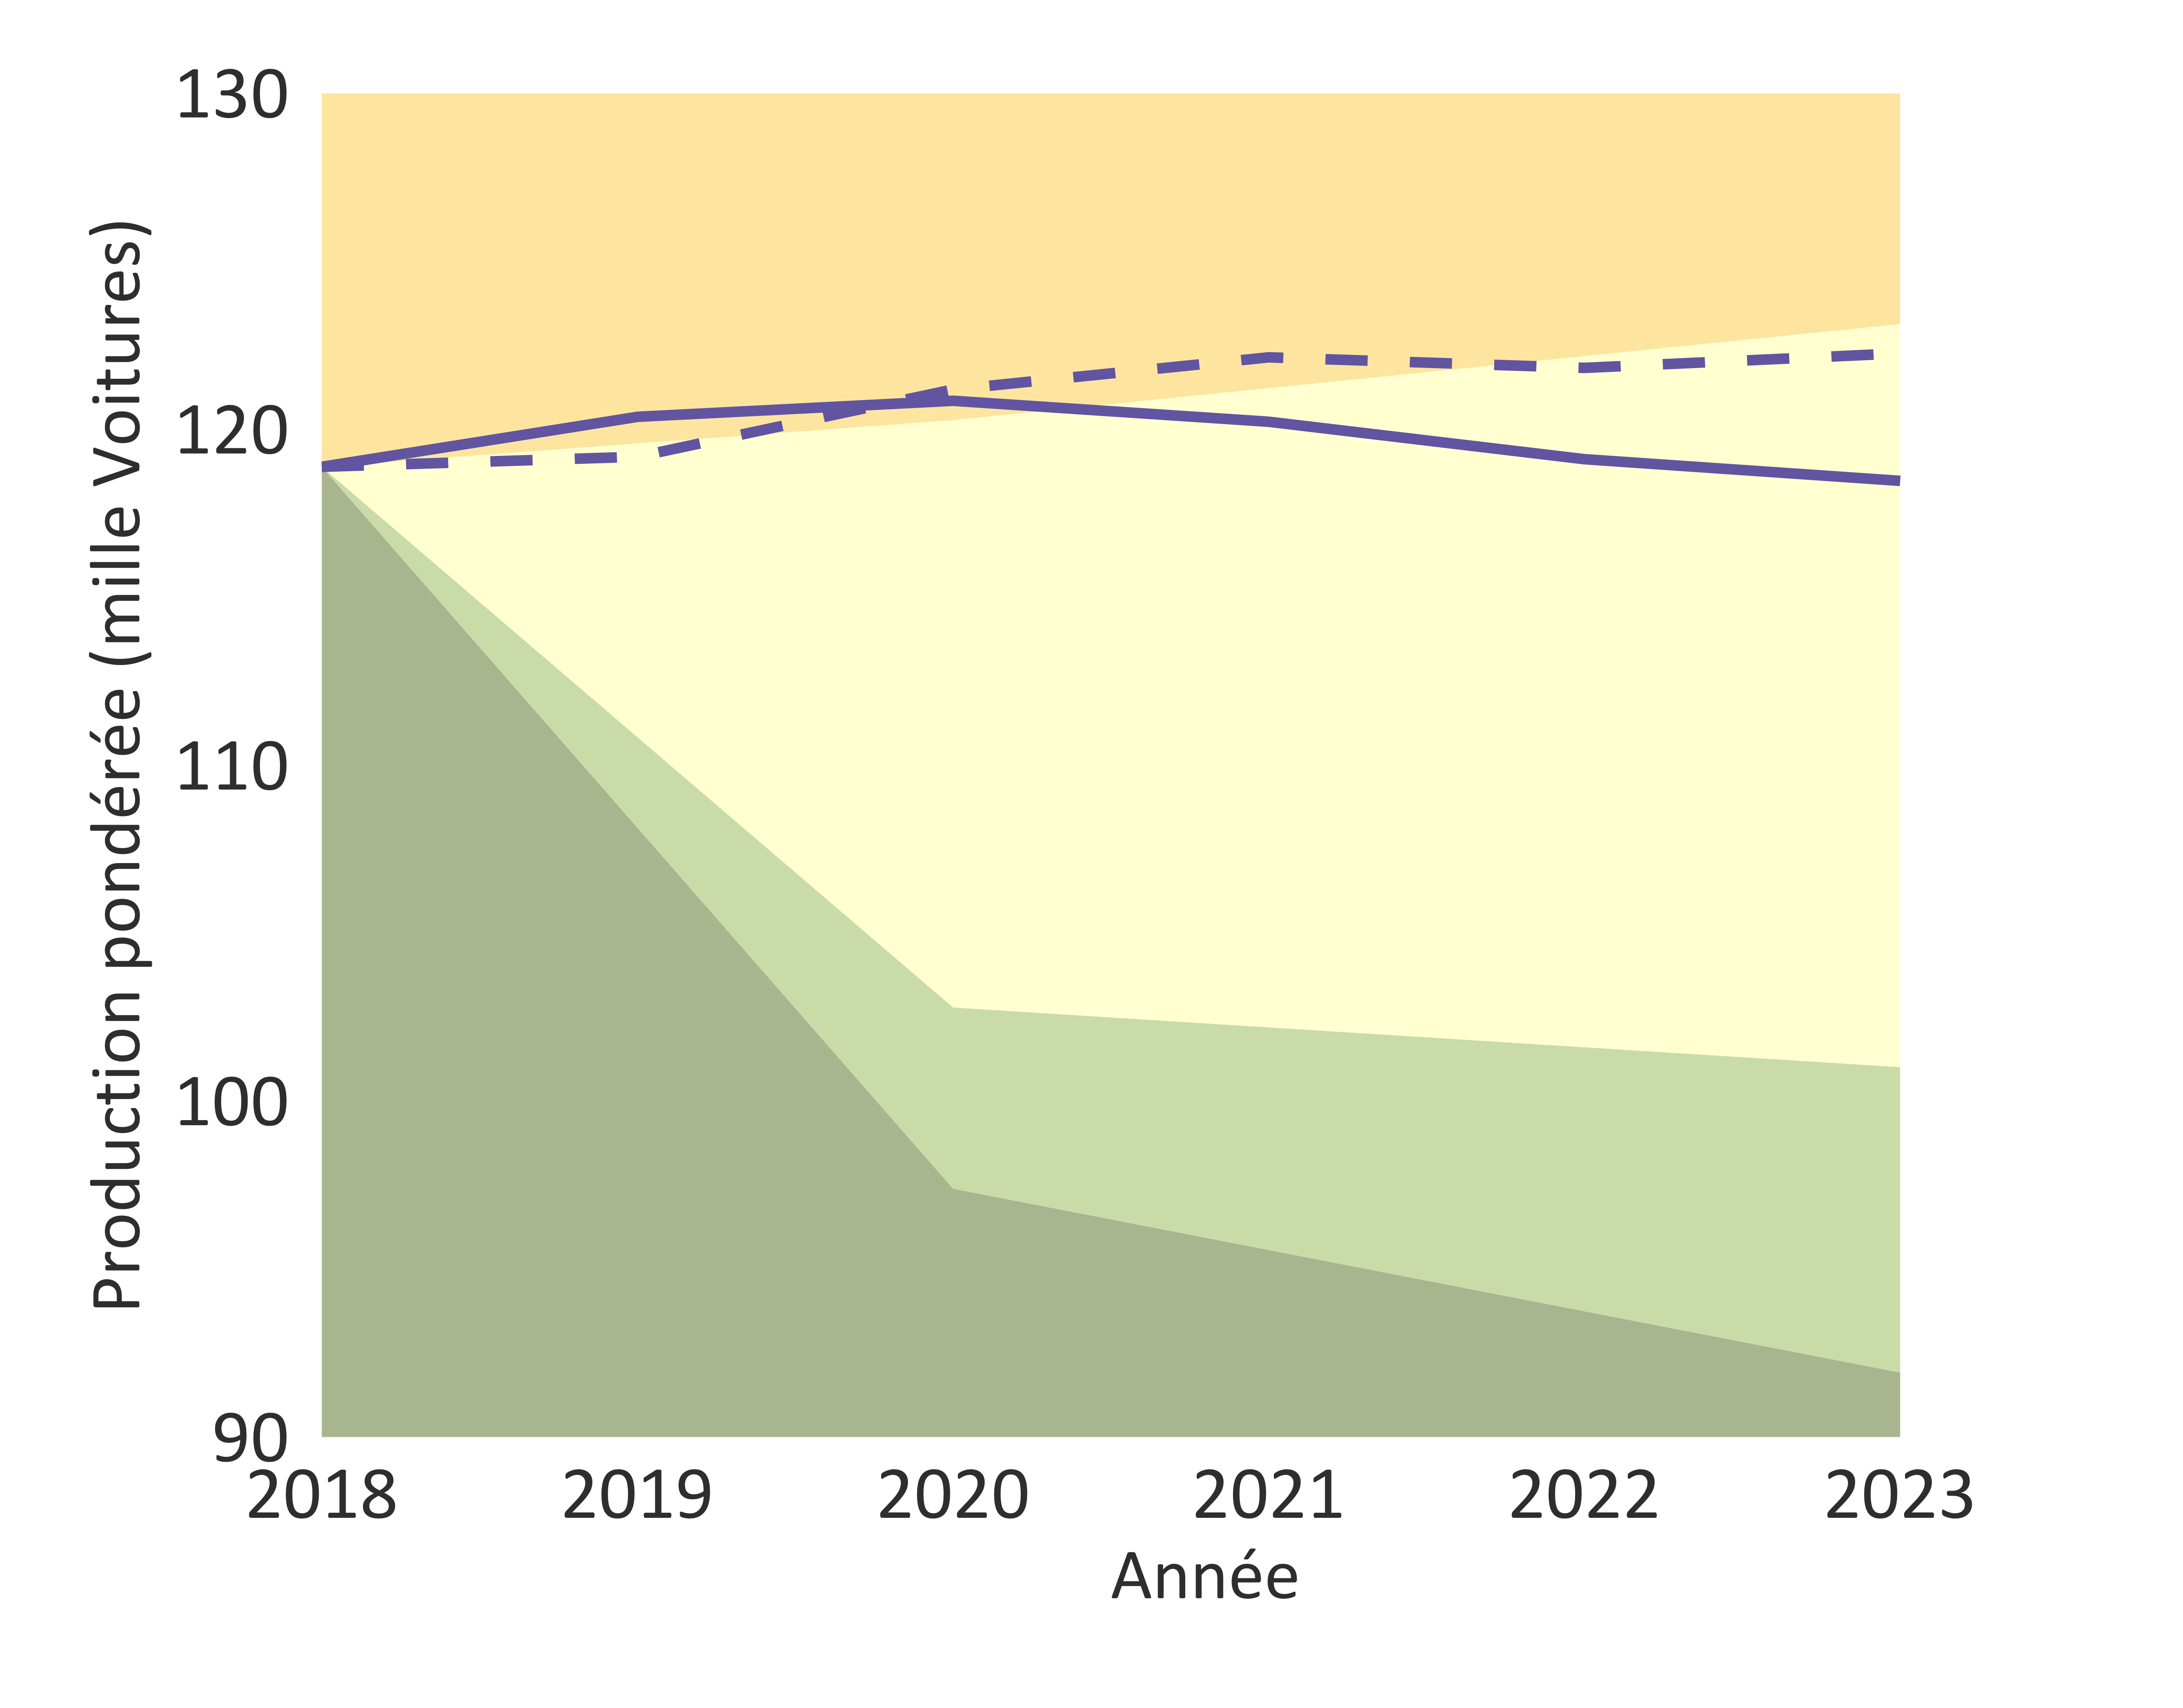
\includegraphics[trim = {0 0cm 0 0},width=1\linewidth]{ReportOutputs/Fig14}
		
	\end{minipage}	
	\hspace{.02\linewidth}
	\begin{minipage}[t]{.49\textwidth}
		\textbf{Trayectoria de Producción de Vehículos Eléctricos}
		
		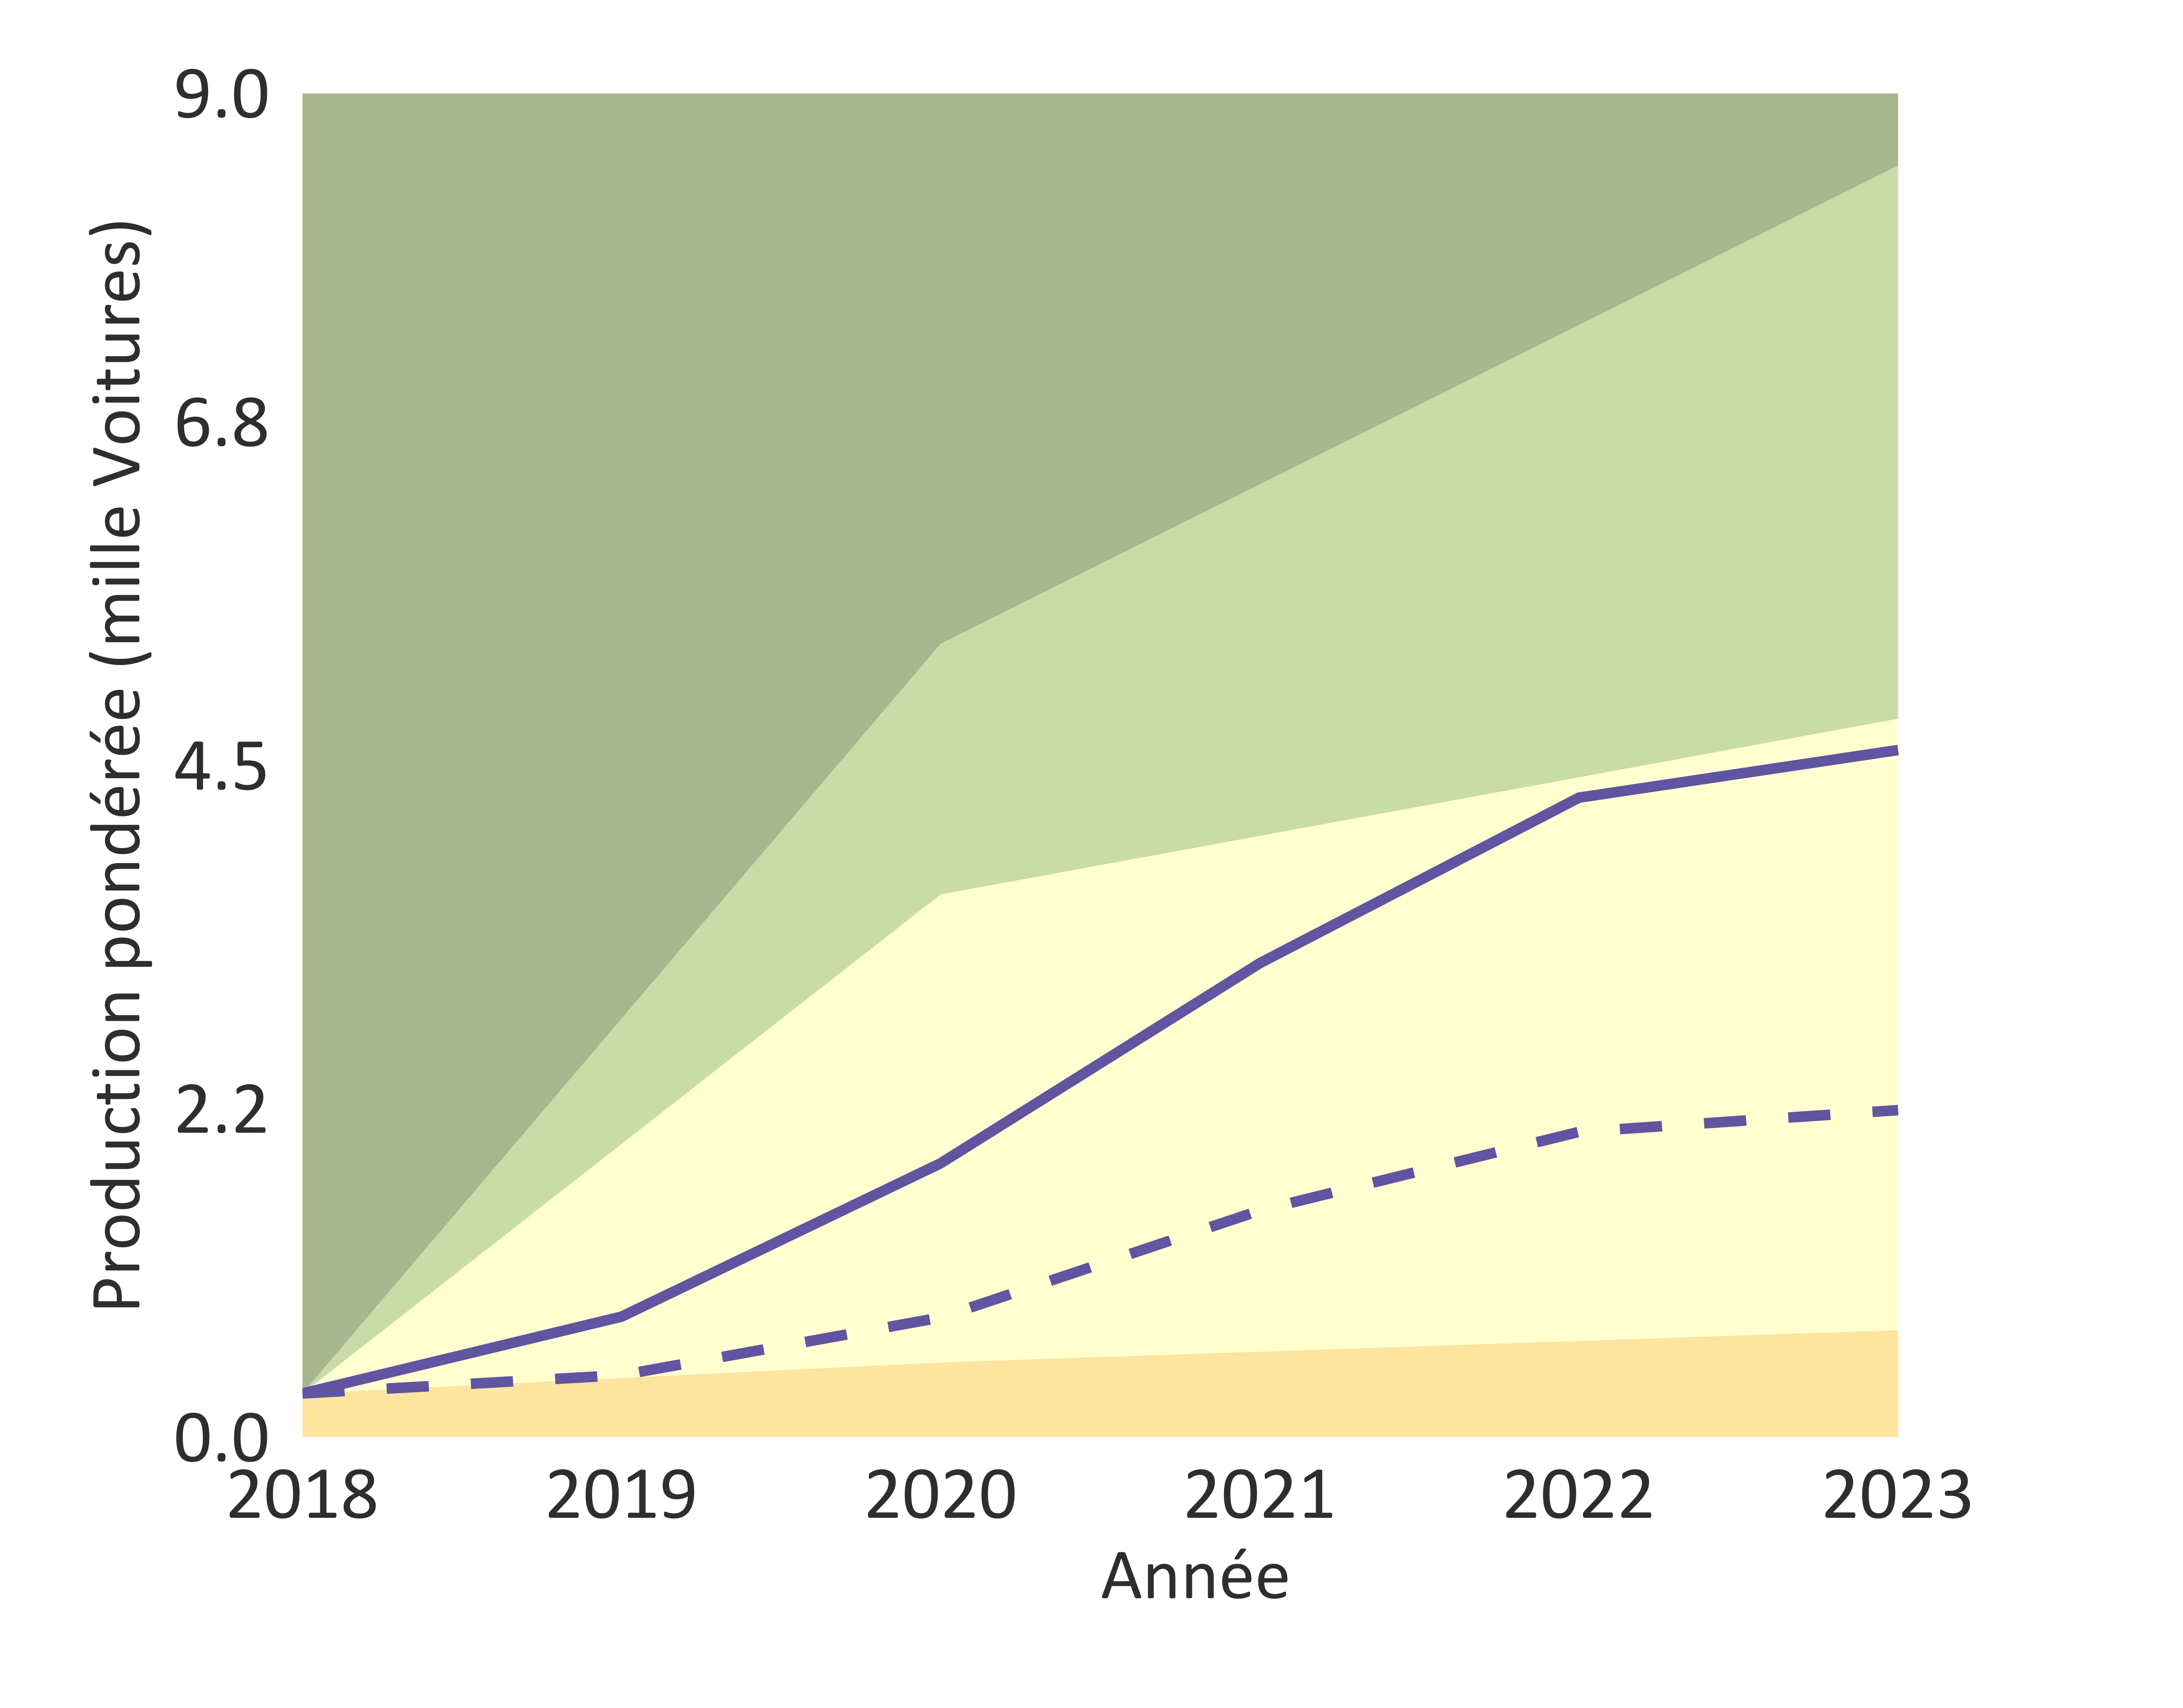
\includegraphics[trim = {0 0cm 0 0},width=1\linewidth]{ReportOutputs/Fig15}
		
	\end{minipage}	

	\begin{minipage}[t]{.49\textwidth}
		\textbf{Trayectoria de Producción de Vehículos Híbridos}
	
		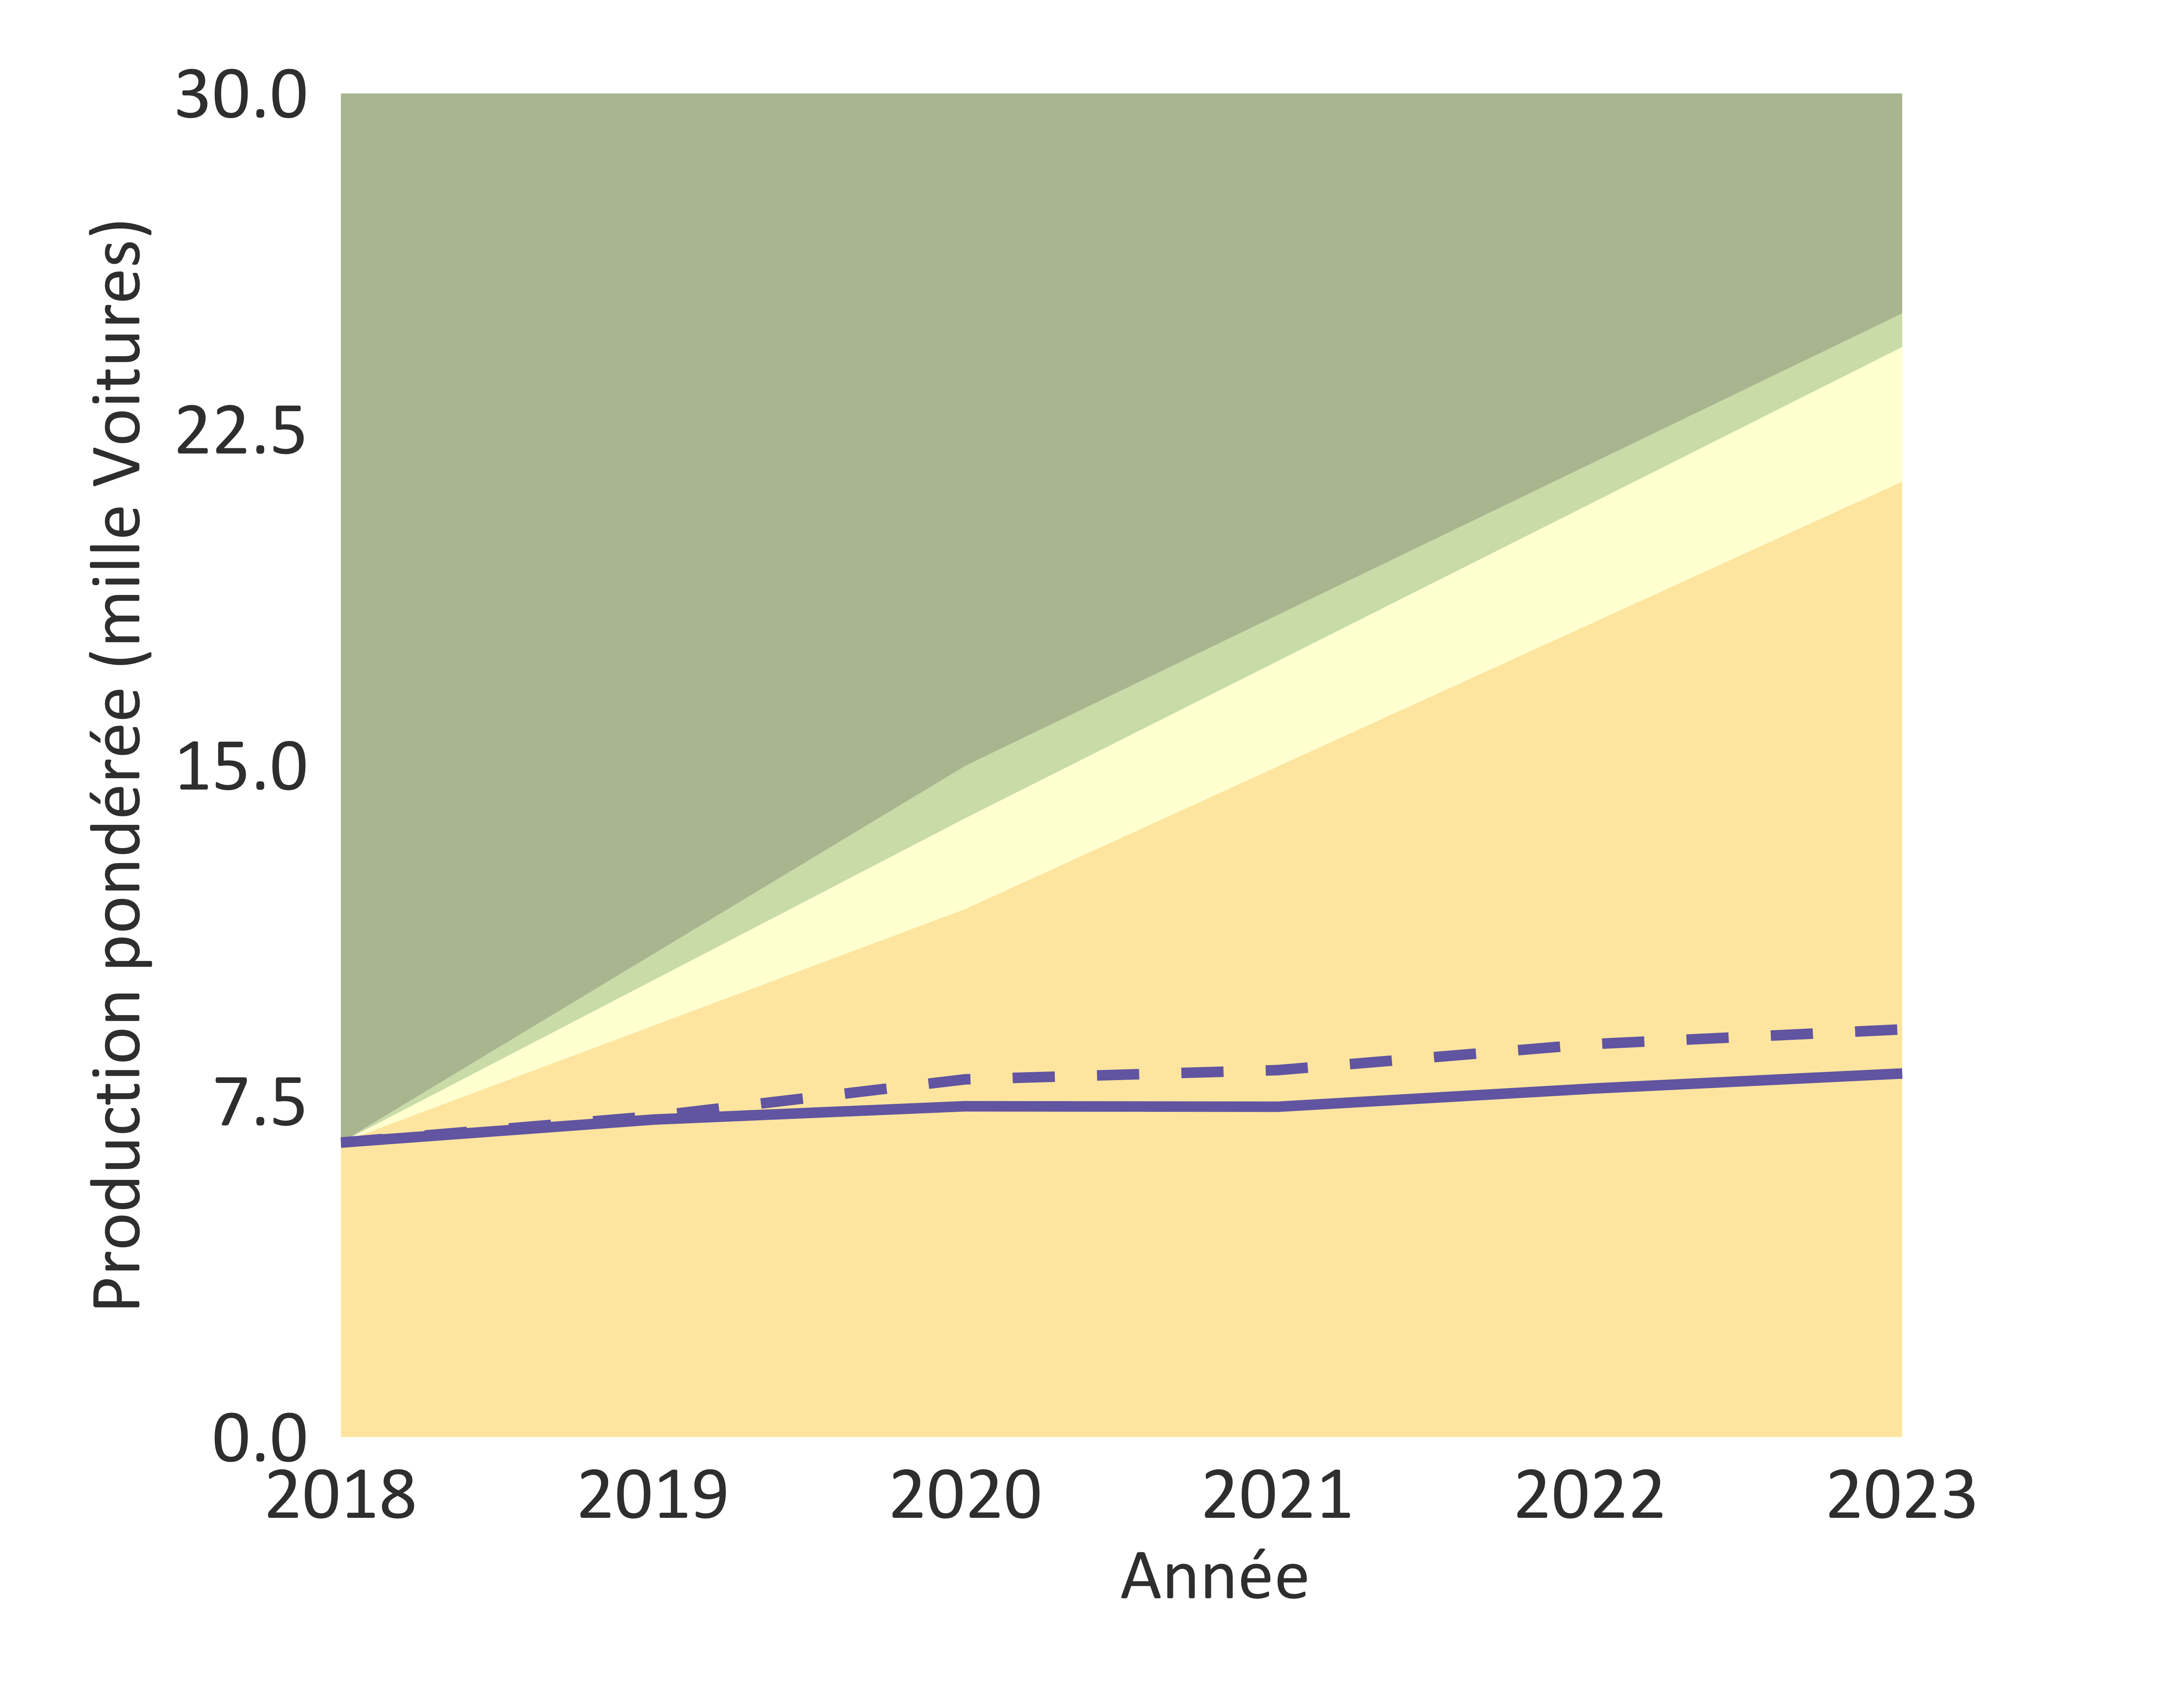
\includegraphics[trim = {0 0cm 0 0},width=1\linewidth]{ReportOutputs/Fig16}
	
	\end{minipage}		
	
	\vspace{-.6cm}
	\begin{center}
		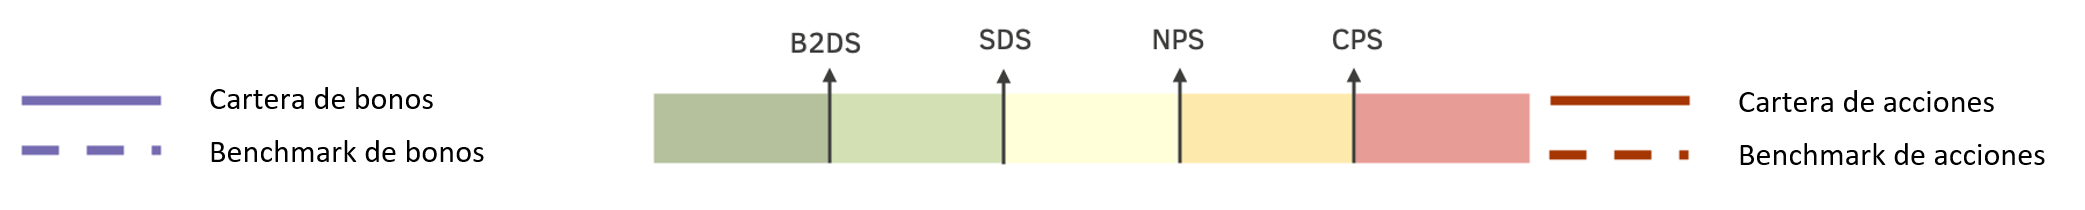
\includegraphics[trim = {0 0cm 0 0},width=.9\linewidth]{ReportGraphics/246Legend_ES.png}
	\end{center}
	

	%\PageFooterThird
\PageFooter{3 - TRAYECTORIA DE LA CARTERA}
	
	\newpage 
	%AutoSector_CBE 
	%AutoSector_EQS	
	\section*{} % TRAJECTORY - EQUITY - FOSSIL FUELS AND AUTOMOTIVE 
		\HeaderDouble{TENDENCIA A 5 AÑOS – ACCIONES}{SECTOR AUTOMOTRIZ}	
	
	\begin{multicols}{2}
		\textbf{Los gráficos de alineación a continuación muestran la alineación de tecnologías automotrices en la cartera de acciones respecto a los escenarios de transición de la AIE: B2DS, SDS, NPS, CPS y la alineación del mercado de acciones. } 
		Para cada tecnología, el valor graficado de la cartera (línea continua) representa la evolución estimada o “trayectoria” de la producción automotriz atribuida a la cartera de acciones en los próximos 5 años.  Las líneas que separan las áreas del fondo codificado por colores representan la “producción objetivo” de la cartera para cada tecnología bajo los escenarios de la AIE. La línea punteada representa la trayectoria planeada por tecnología en el mercado de acciones, ajustada al mismo punto de inicio de la cartera.          
		
	\end{multicols}		
	
	
	\begin{minipage}[t]{.49\linewidth}
		\textbf{Trayectoria de Producción de Vehículos de Combustión Interna}
		
		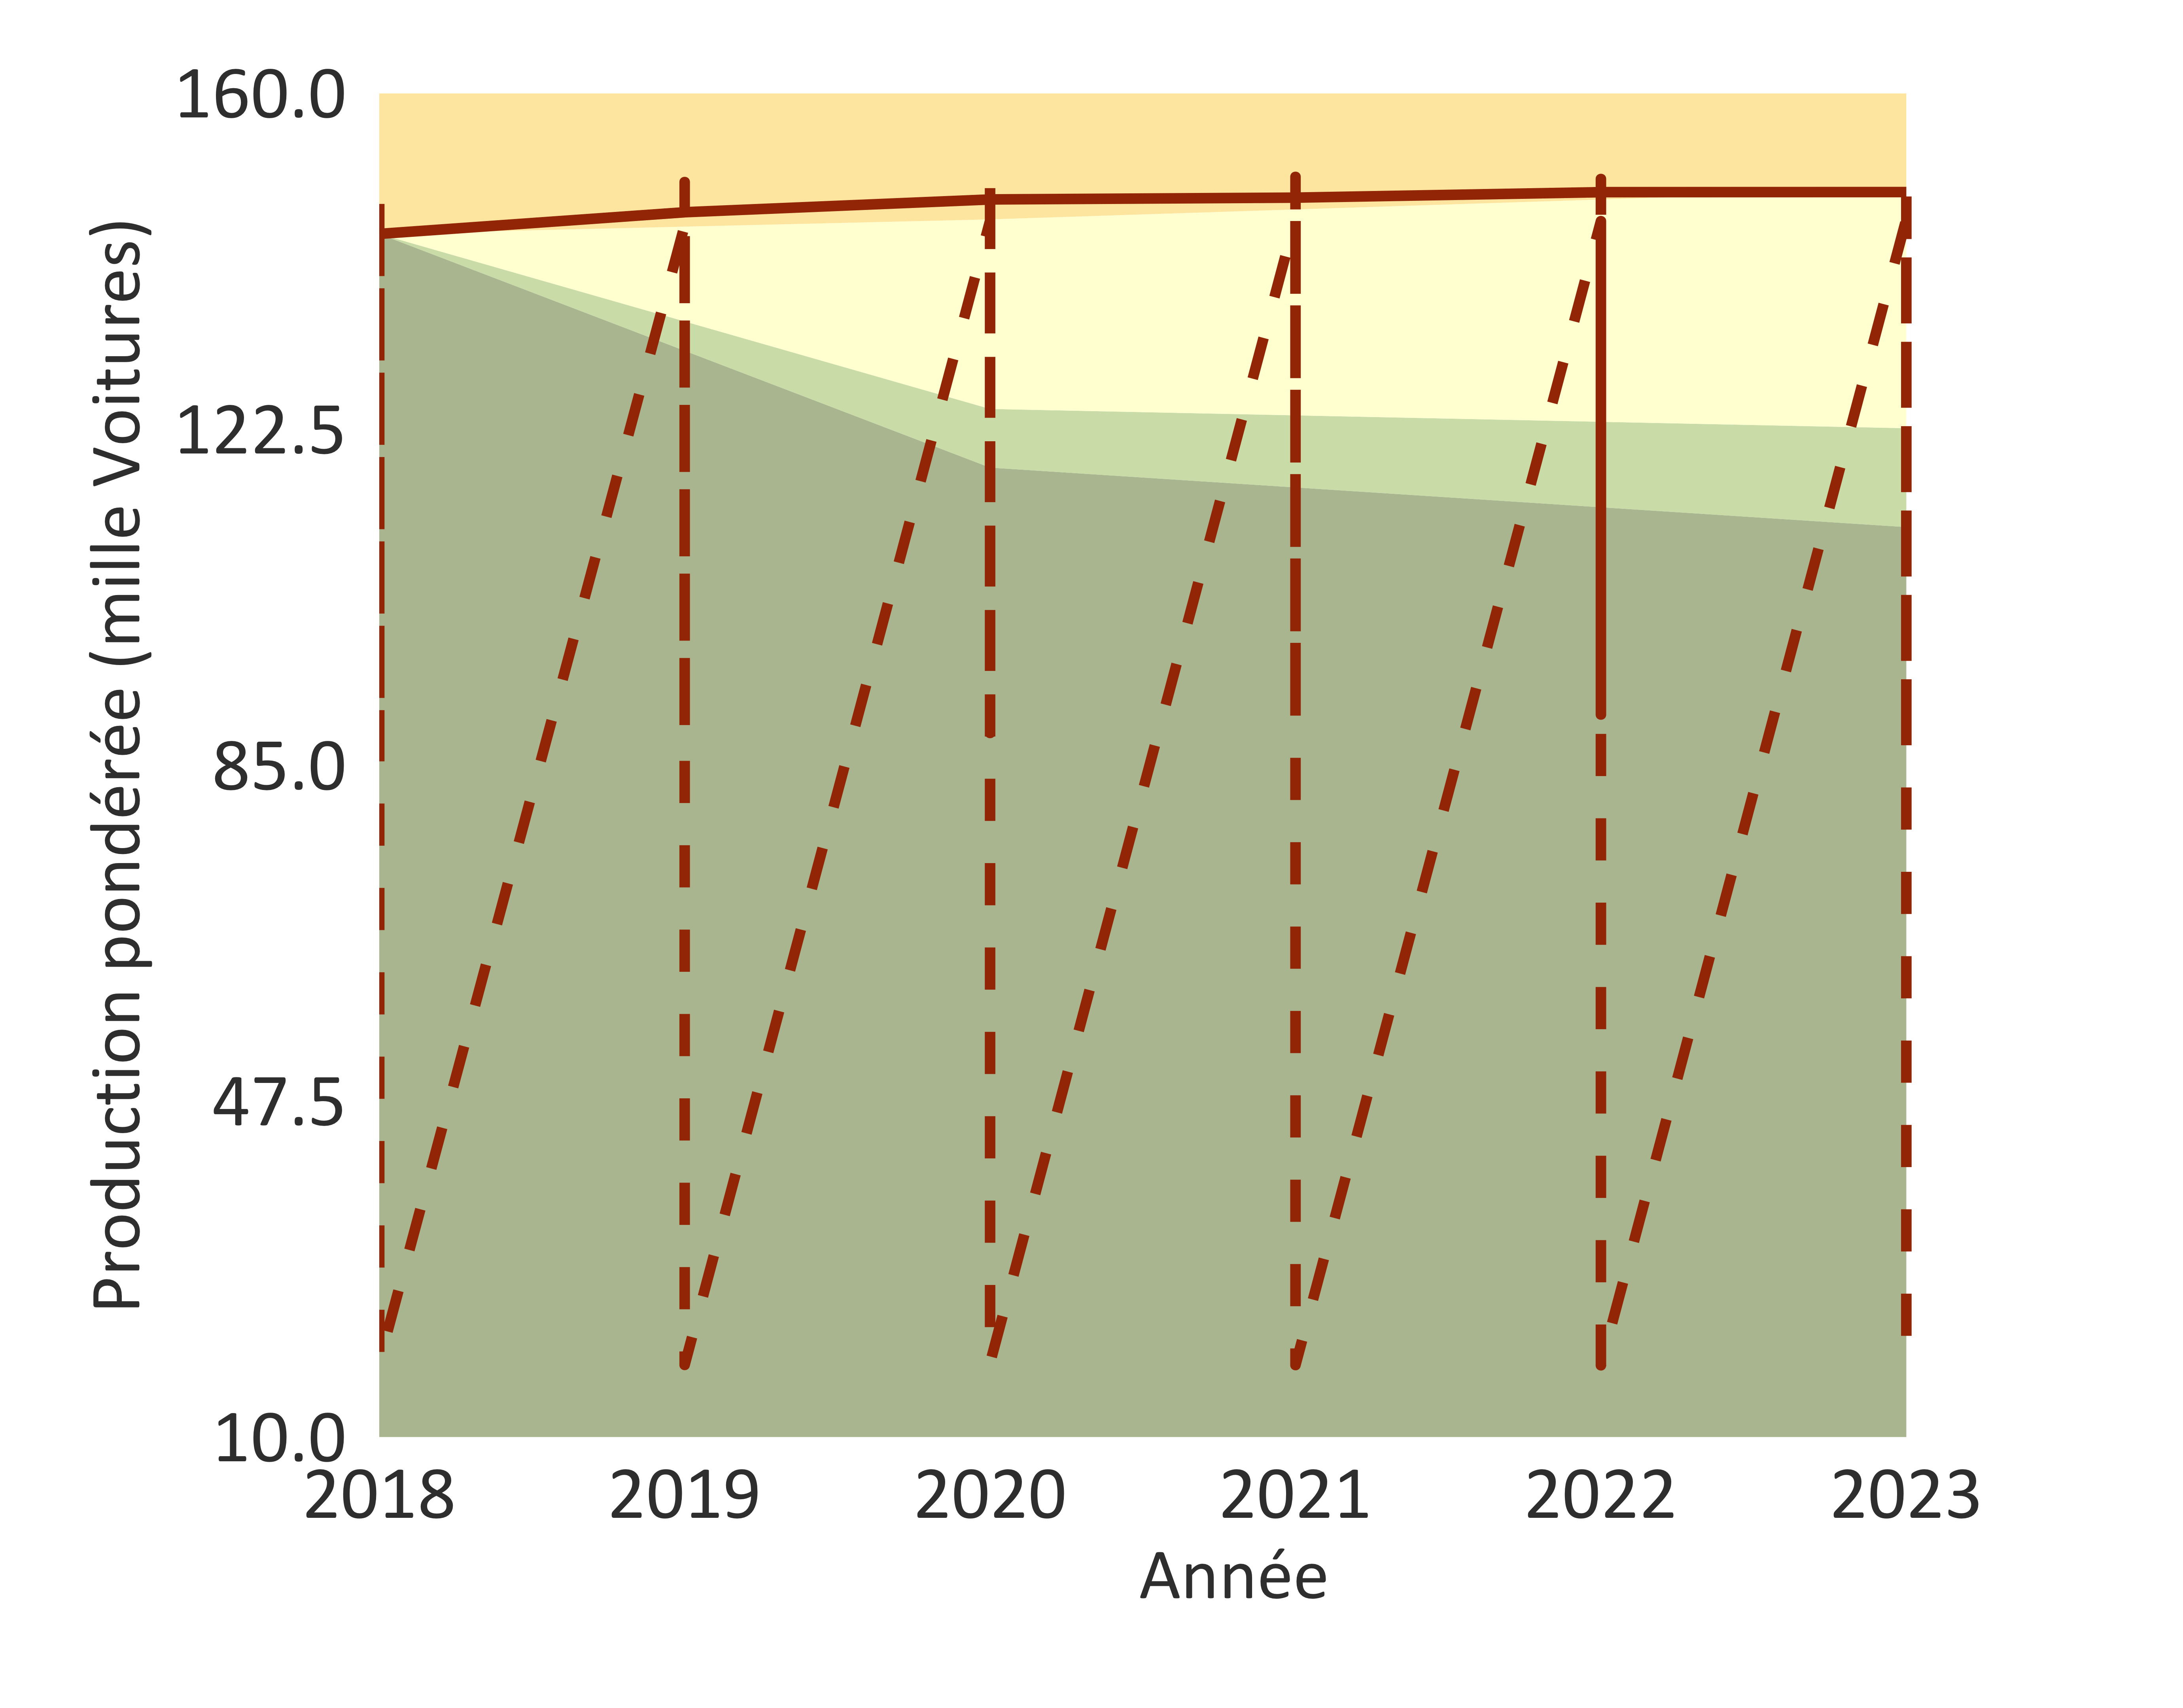
\includegraphics[trim = {0 0cm 0 0},width=1\linewidth]{ReportOutputs/Fig24}
		
	\end{minipage}	
	\hspace{.02\linewidth}
	\begin{minipage}[t]{.49\textwidth}
		\textbf{Trayectoria de Producción de Vehículos Eléctricos}
		
		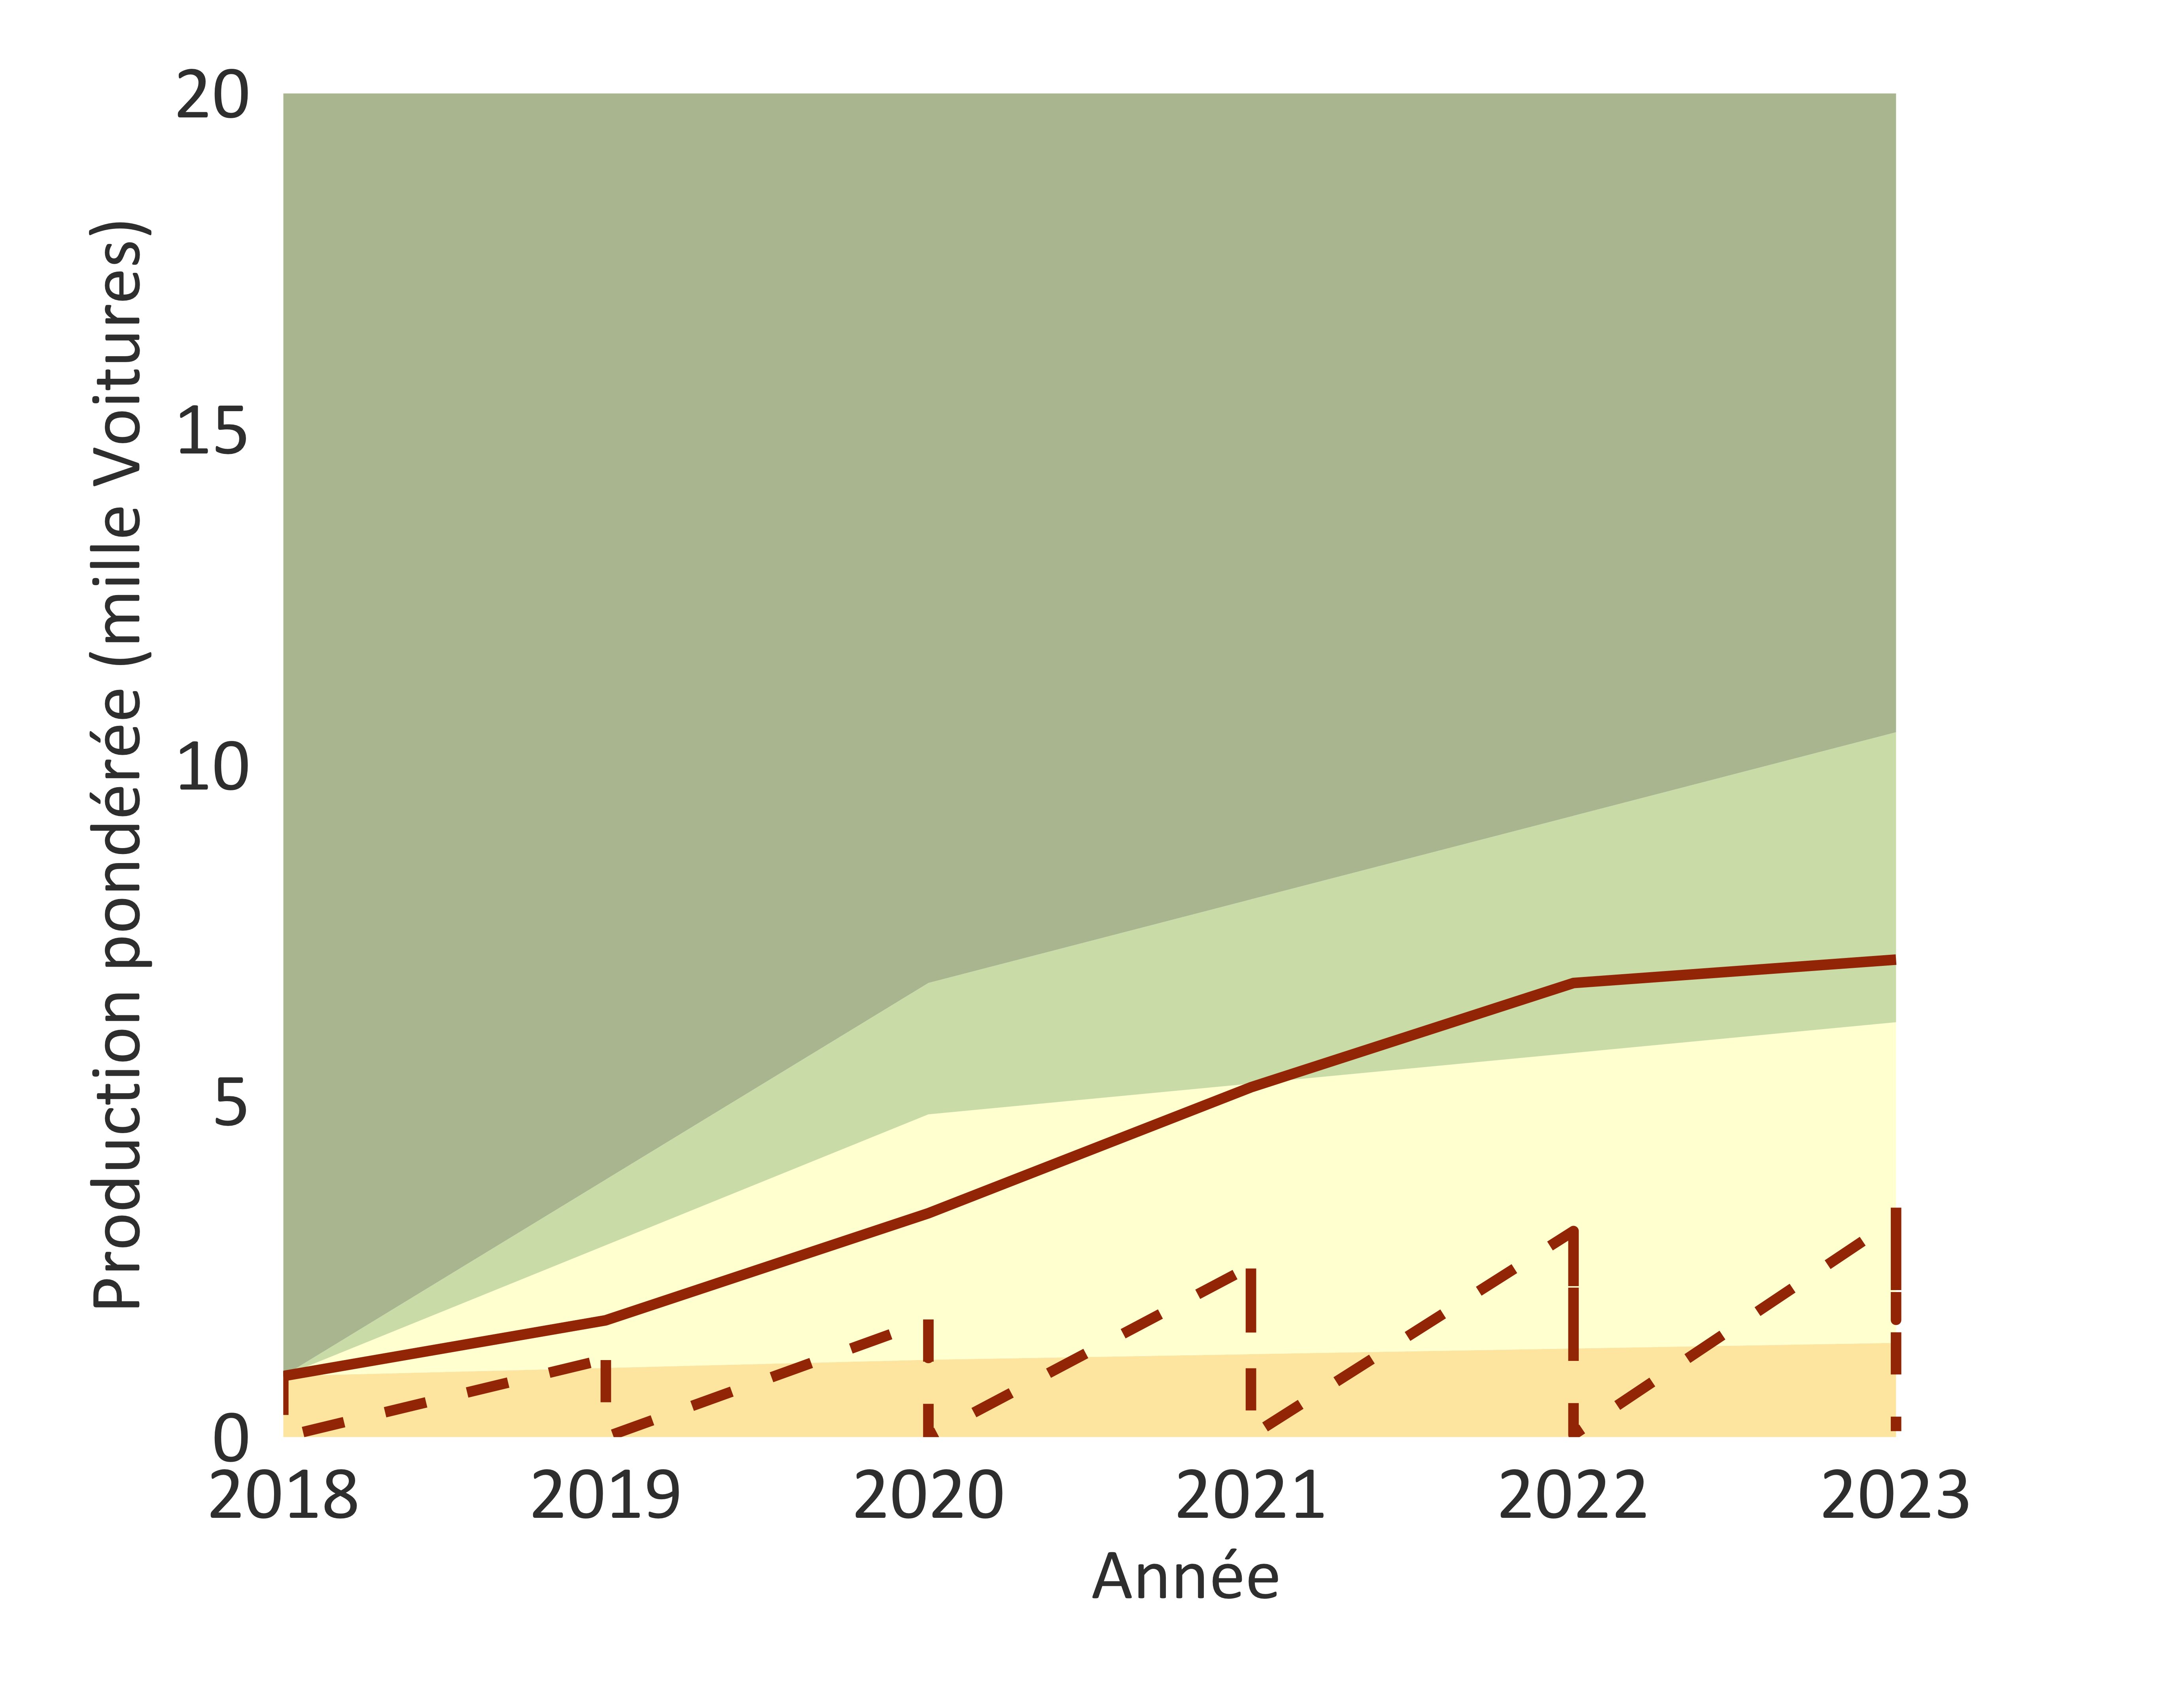
\includegraphics[trim = {0 0cm 0 0},width=1\linewidth]{ReportOutputs/Fig25}
		
	\end{minipage}	
	
	\begin{minipage}[t]{.49\textwidth}
		\textbf{Trayectoria de Producción de Vehículos Híbridos}
		
		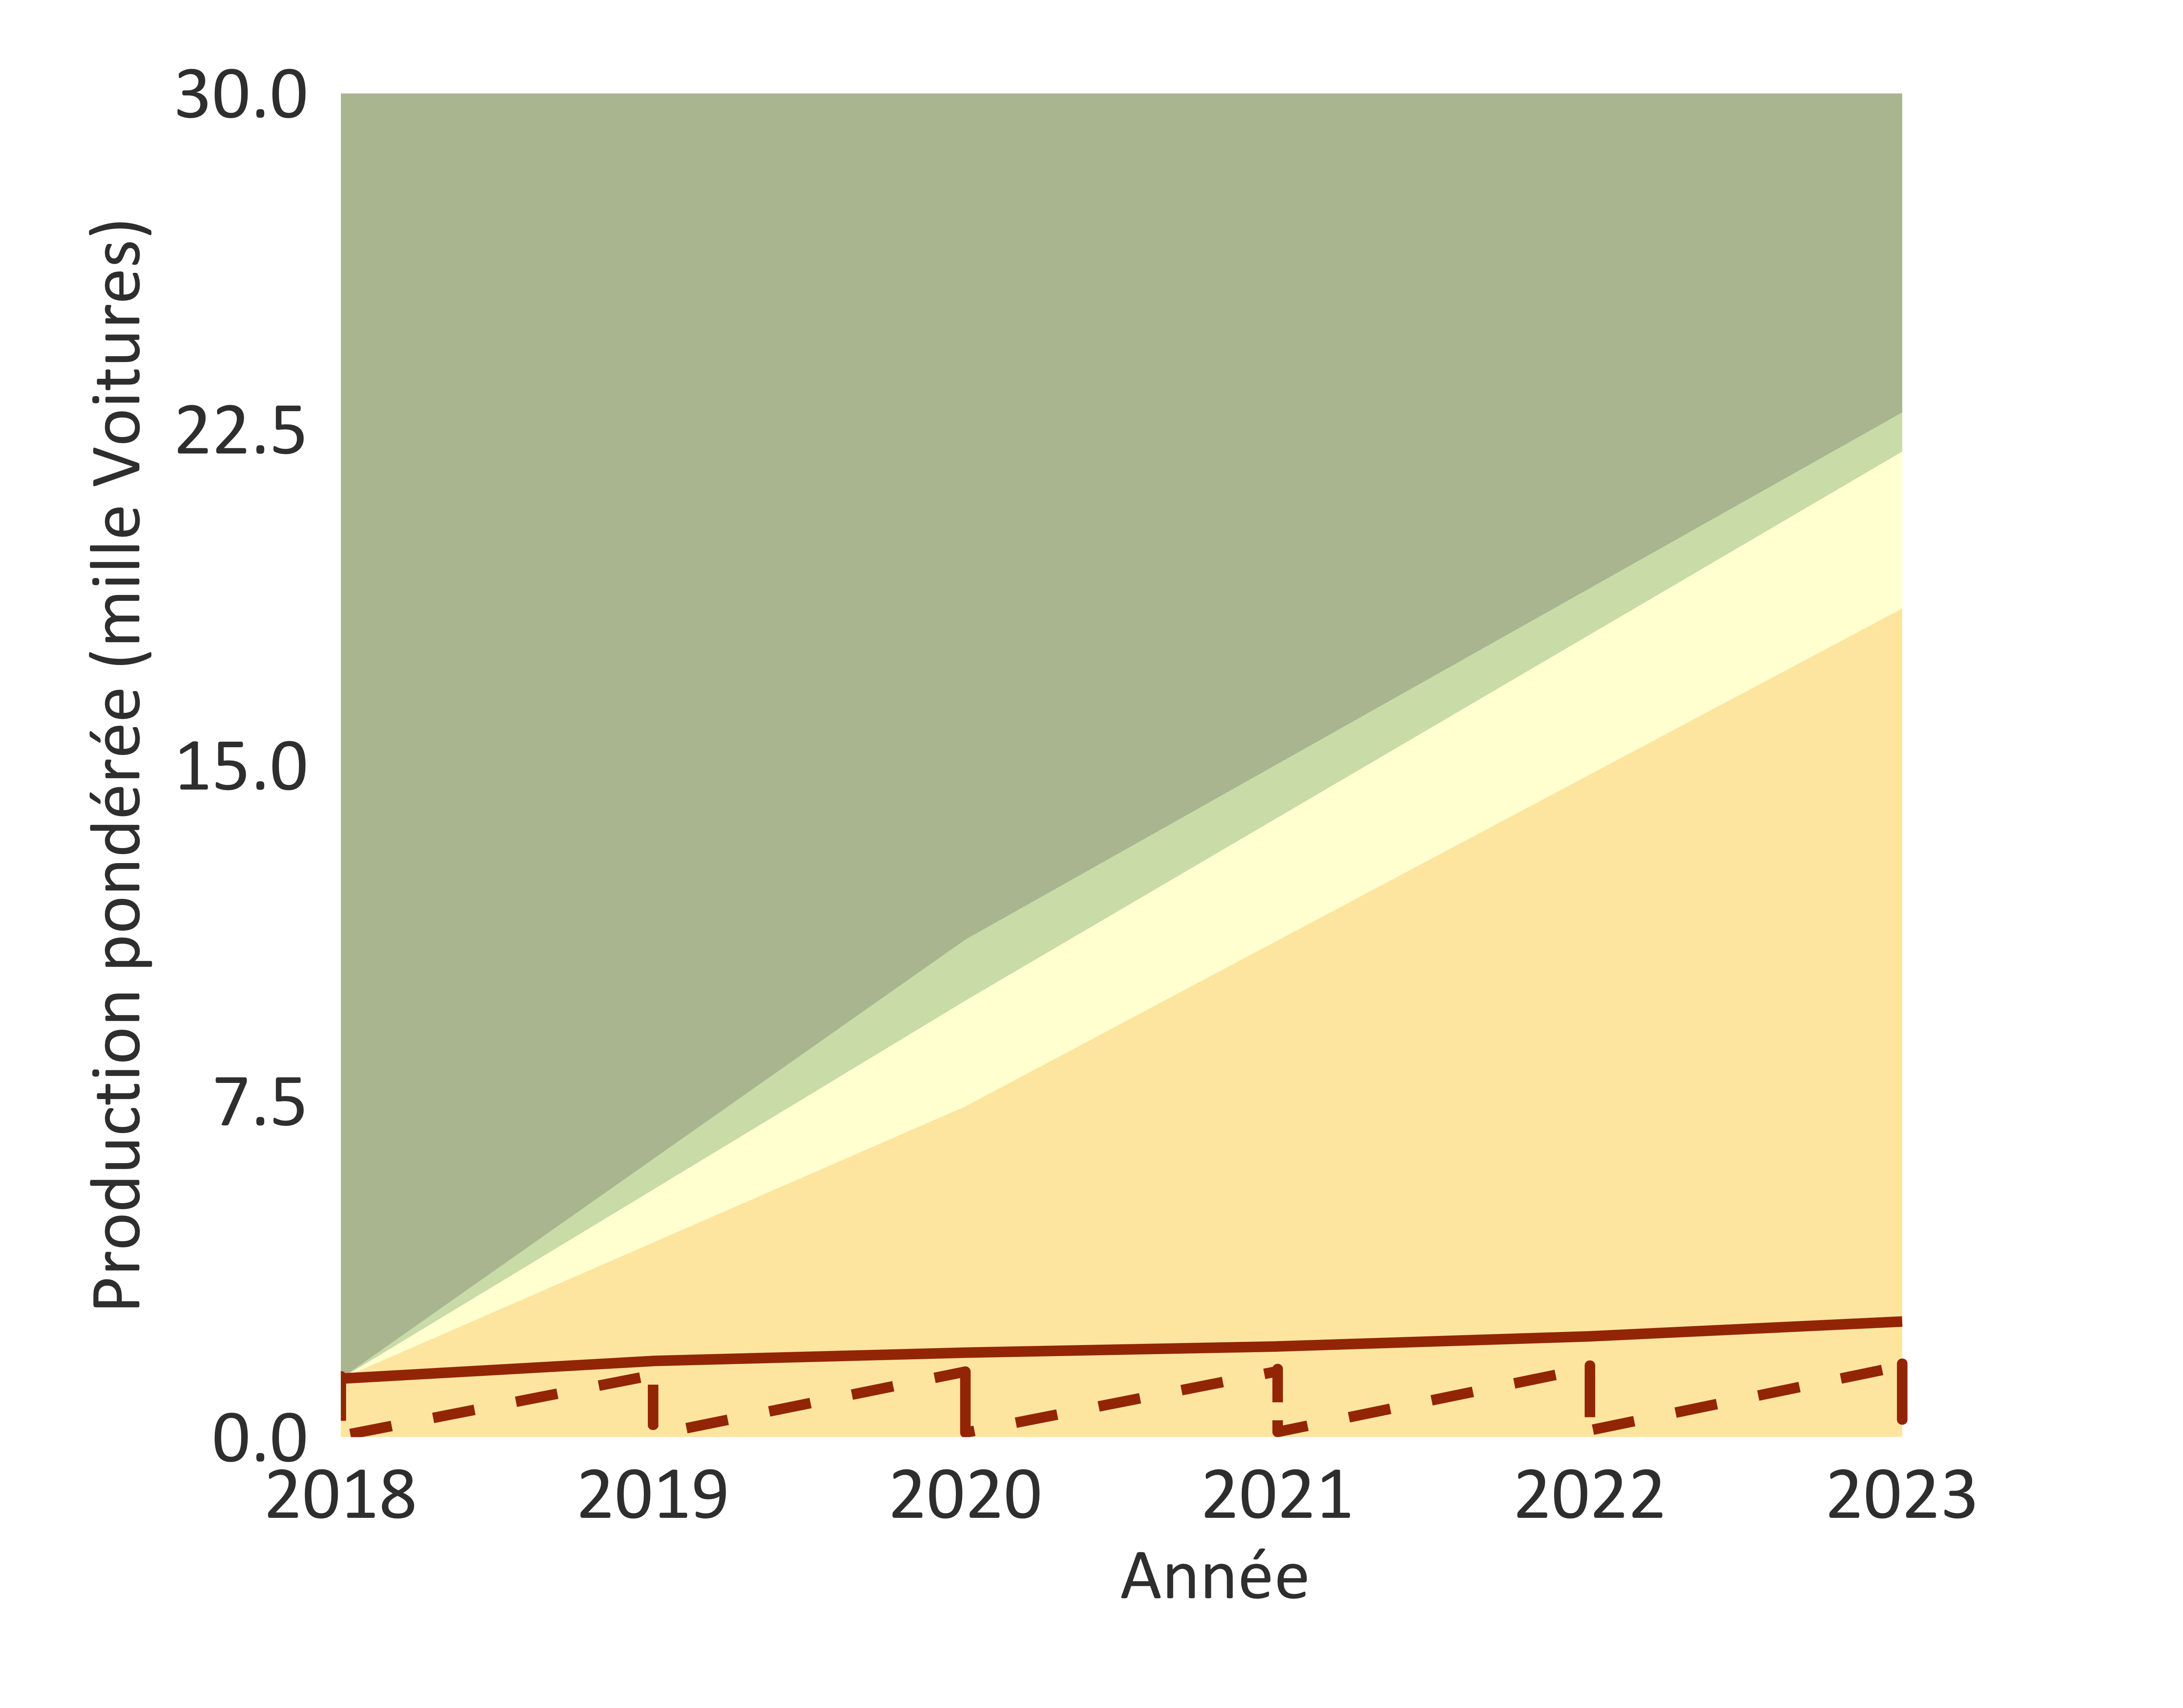
\includegraphics[trim = {0 0cm 0 0},width=1\linewidth]{ReportOutputs/Fig26}
		
	\end{minipage}		
	
	\vspace{-.6cm}
	\begin{center}
		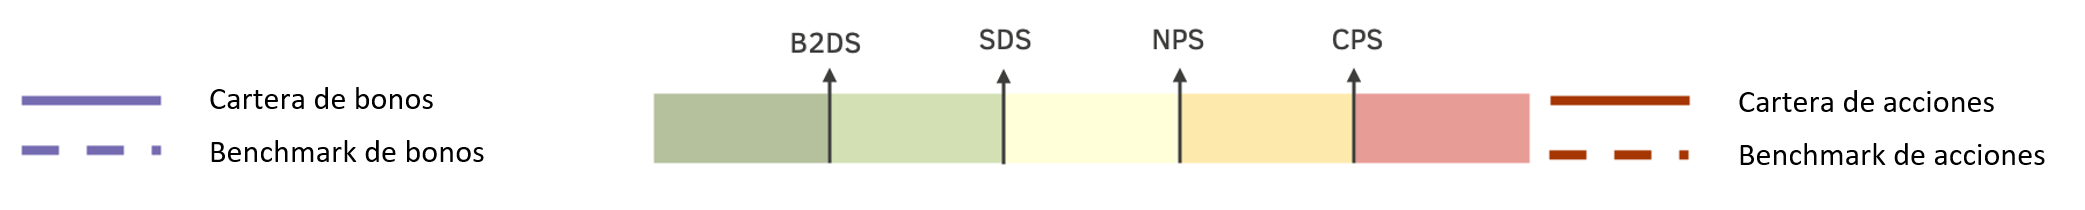
\includegraphics[trim = {0 0cm 0 0},width=.9\linewidth]{ReportGraphics/246Legend_ES.png}
	\end{center}
	
	
	%\PageFooterThird
\PageFooter{3 - TRAYECTORIA DE LA CARTERA}
	
	\newpage 
	%AutoSector_EQE
	%AutoSector_ALLE
	%OtherSectorsS
	\section*{} % OTHER SECTORS 
	\HeaderSingle{ANÁLISIS DE INTENSIDAD DE EMISIONES}
	
	\begin{multicols}{2}
		Hay una gran variedad de sectores para los cuales no existen tecnologías sustitutas bajas en carbono a escala en el mercado o en los cuales los datos a nivel de activos físicos o escenarios son escasos.  Esto es más relevante para los sectores de acero, cemento, transporte marítimo y aviación. Para estos sectores se realizó un análisis de los cambios requeridos en la intensidad de emisiones. 
	
		Para estos sectores los esfuerzos de decarbonización consisten en aumentar la eficiencia energética en la producción y el uso, así como también la inversión en investigación y desarrollo en los próximos 5-10 años, para llevar a que alternativas neutras en CO\textsubscript{2} lleguen a la madurez de mercado a mediano plazo. Como resultado de esto, los escenarios y la data para estos sectores es relativamente imprecisa.
		
		
		Las gráficas siguientes se basan en estimaciones externas de la intensidad de emisiones de CO\textsubscript{2}, las cuales se basan en un modelo de estimación de emisiones público desarrollado por 2Dii y la empresa consultora Ernst \& Young. Para el sector de transporte marítimo, se utilizó un modelo externo de clasificación de emisiones de CO\textsubscript{2} desarrollado por Rightship y Carbon War Room. La calificación de A designa la eficiencia mejor en su clase y G la peor de su clase. Debido a que este modelo es estimado externamente y siguiendo un enfoque vertical descendente (top-down), este puede estar ligado a incertidumbres. Estos resultados deben ser considerados como estimaciones, a diferencia del análisis de escenario para los sectores de energía fósiles, electricidad y automotriz. Para más información consultar la sección 7.
		
	\end{multicols}
	
	\begin{multicols}{2}
		
		\textbf{Cemento}
		
		\textbf{Acero}
		
	\end{multicols}
	
	\setlength\multicolsep{0pt}
	\vspace{0cm}
	
	\begin{multicols}{2}
		
		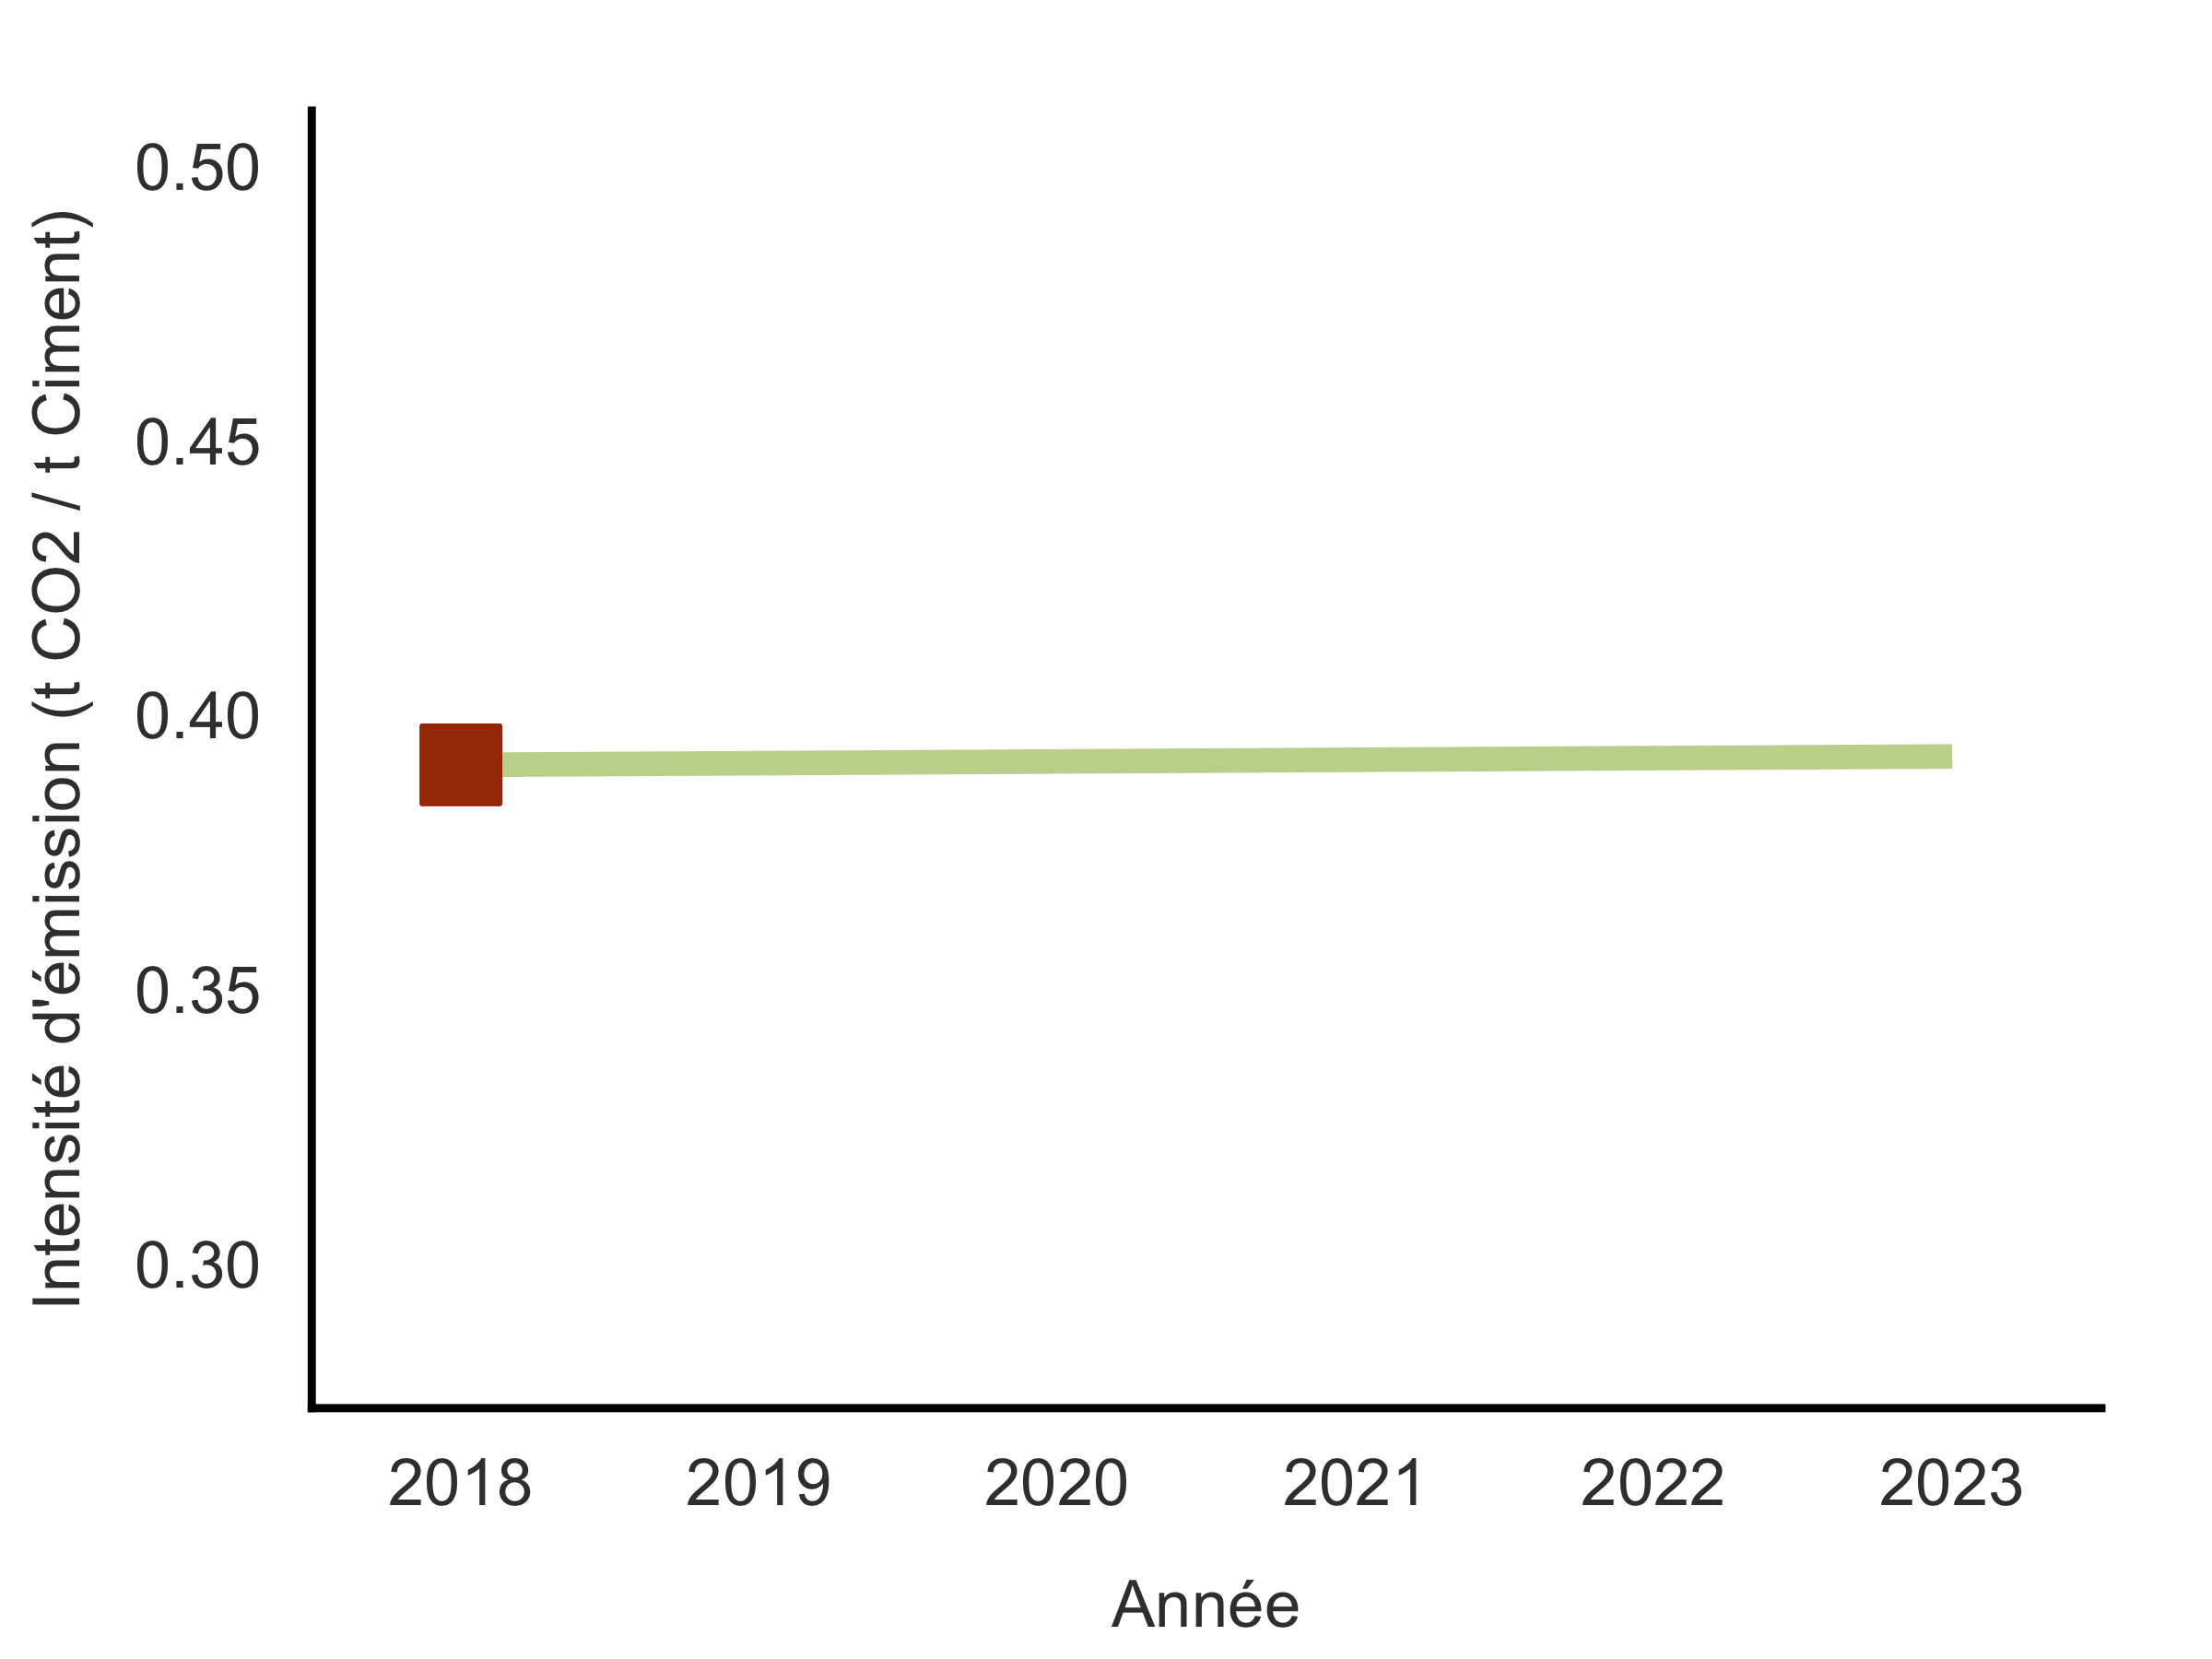
\includegraphics[width=.9\linewidth]{ReportOutputs/Fig30} \vfill\null \columnbreak
		
		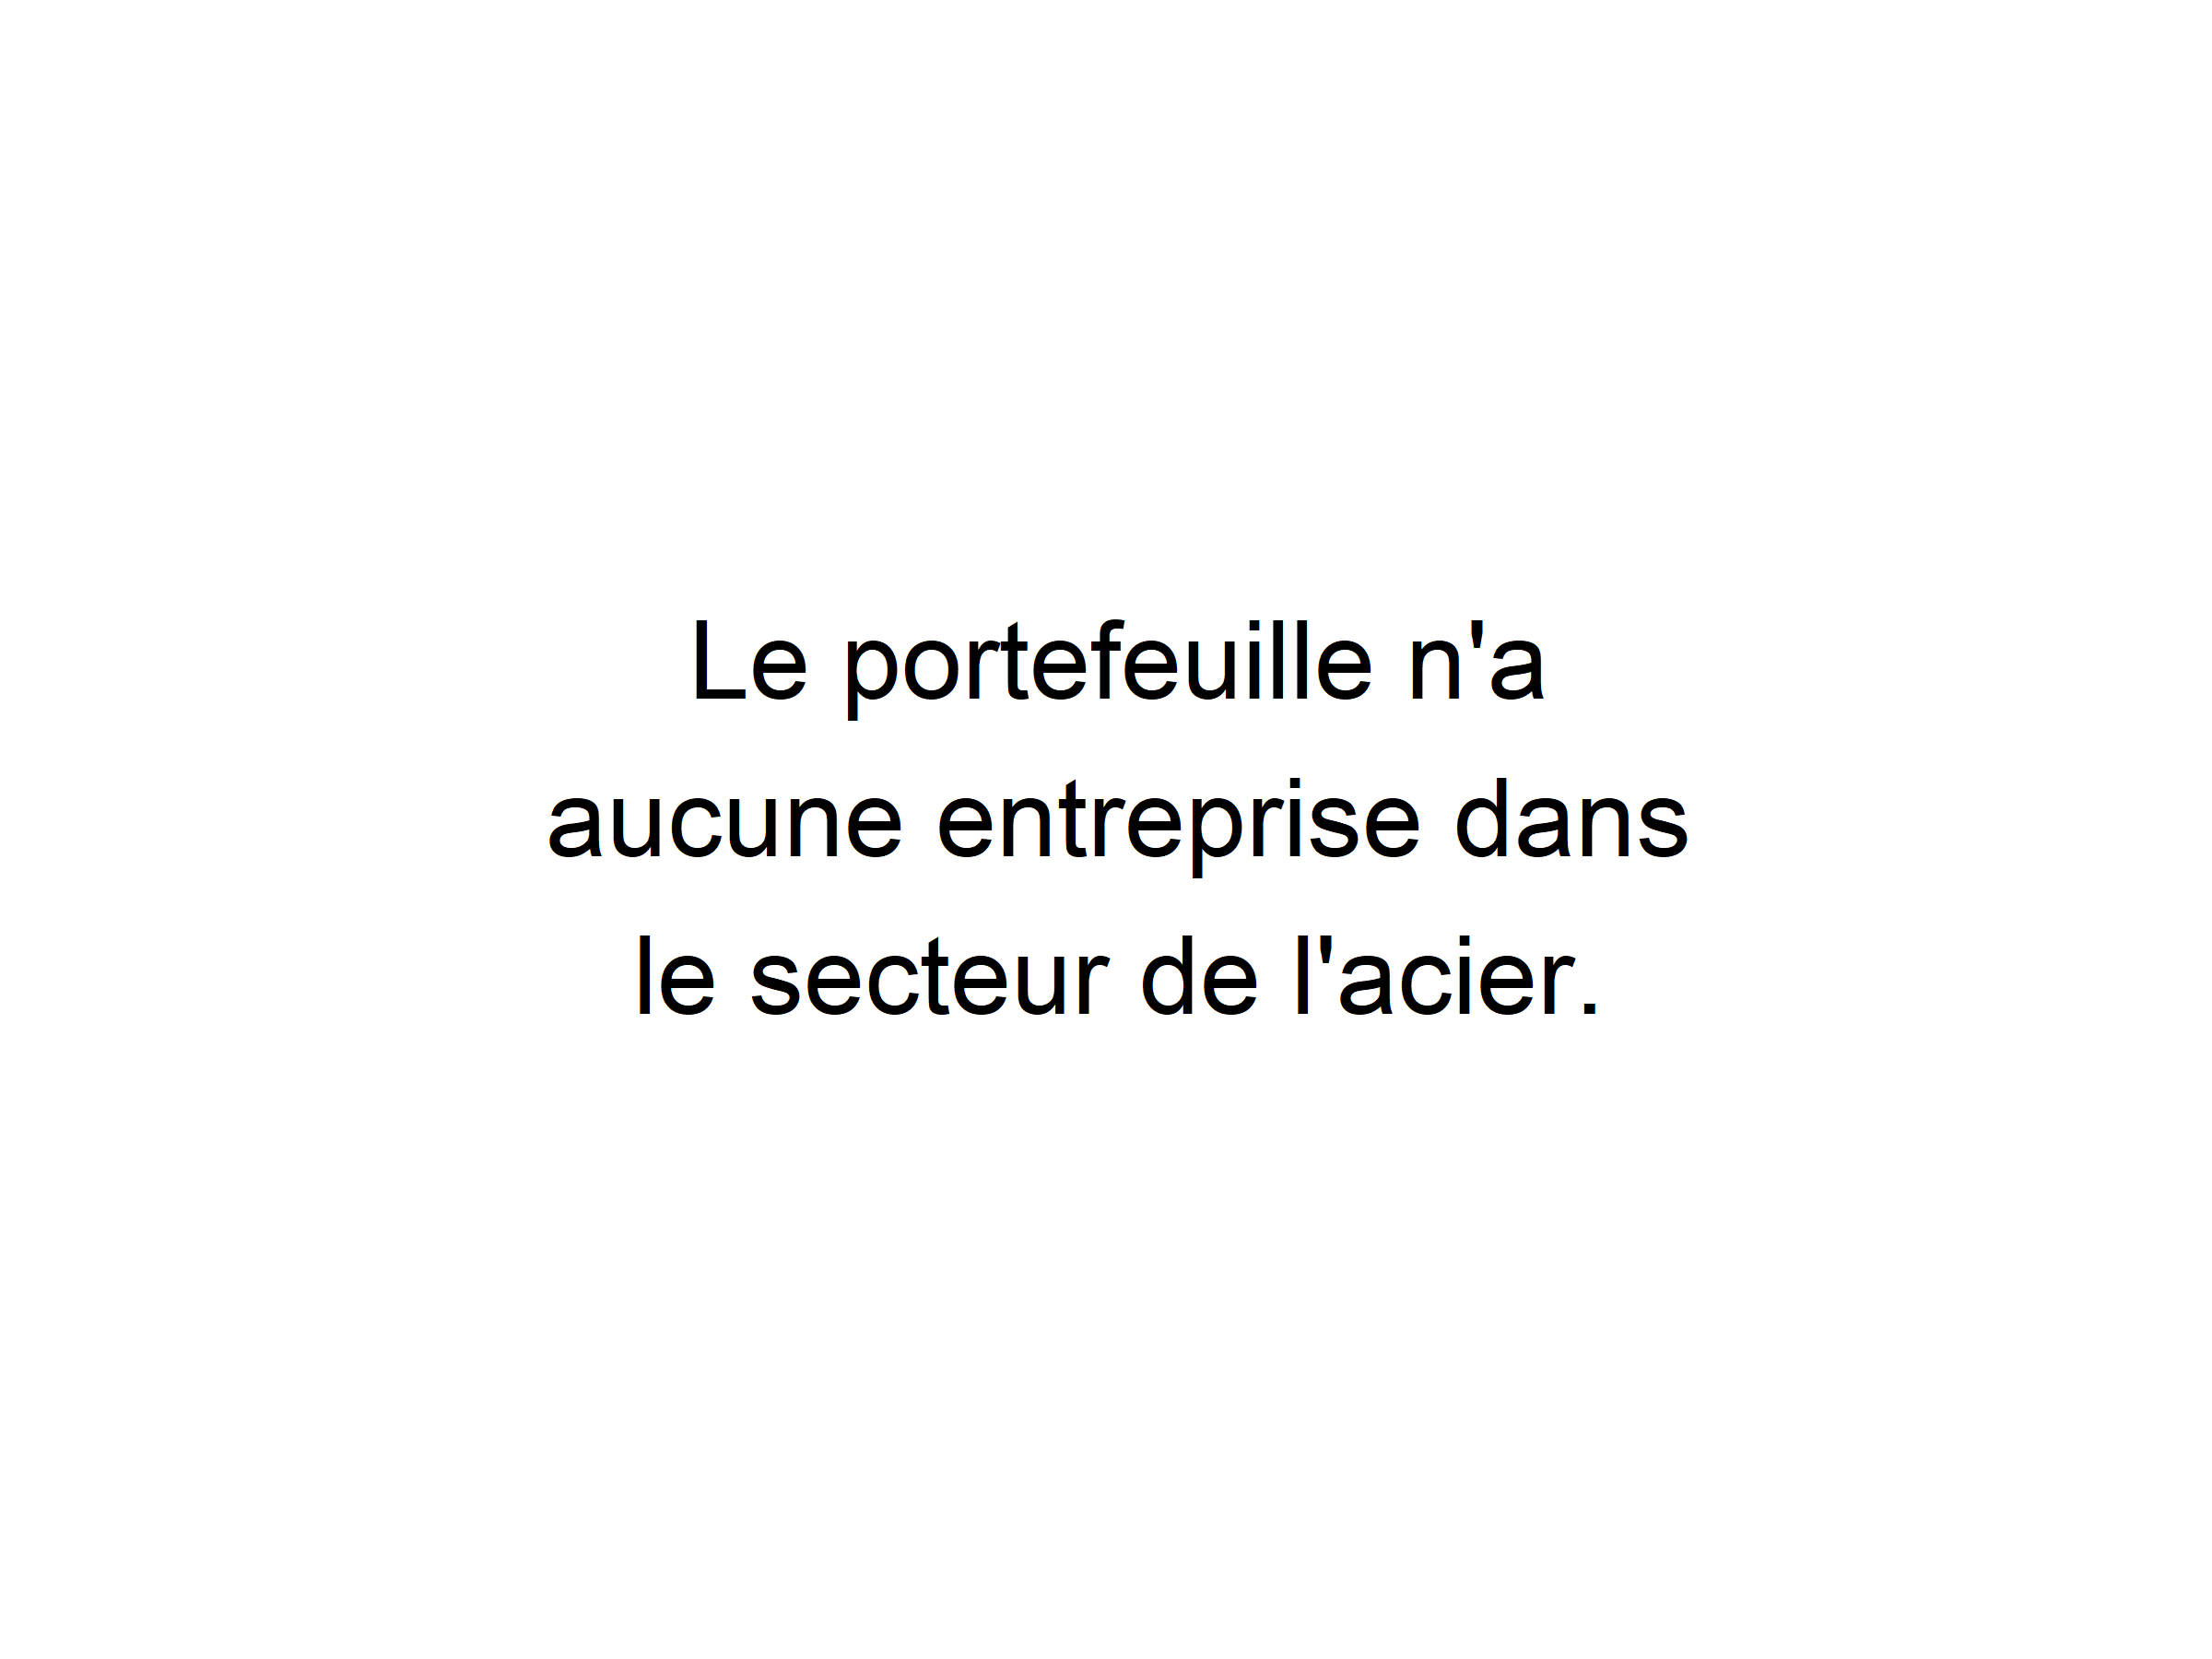
\includegraphics[width=.9\linewidth]{ReportOutputs/Fig31}
		
	\end{multicols}
	
	\begin{multicols}{2}
		
		\textbf{Aviación}
		
		\textbf{Transporte Marítimo}
		
	\end{multicols}
	
	\vspace{0cm}
	
	\begin{multicols}{2}
		
		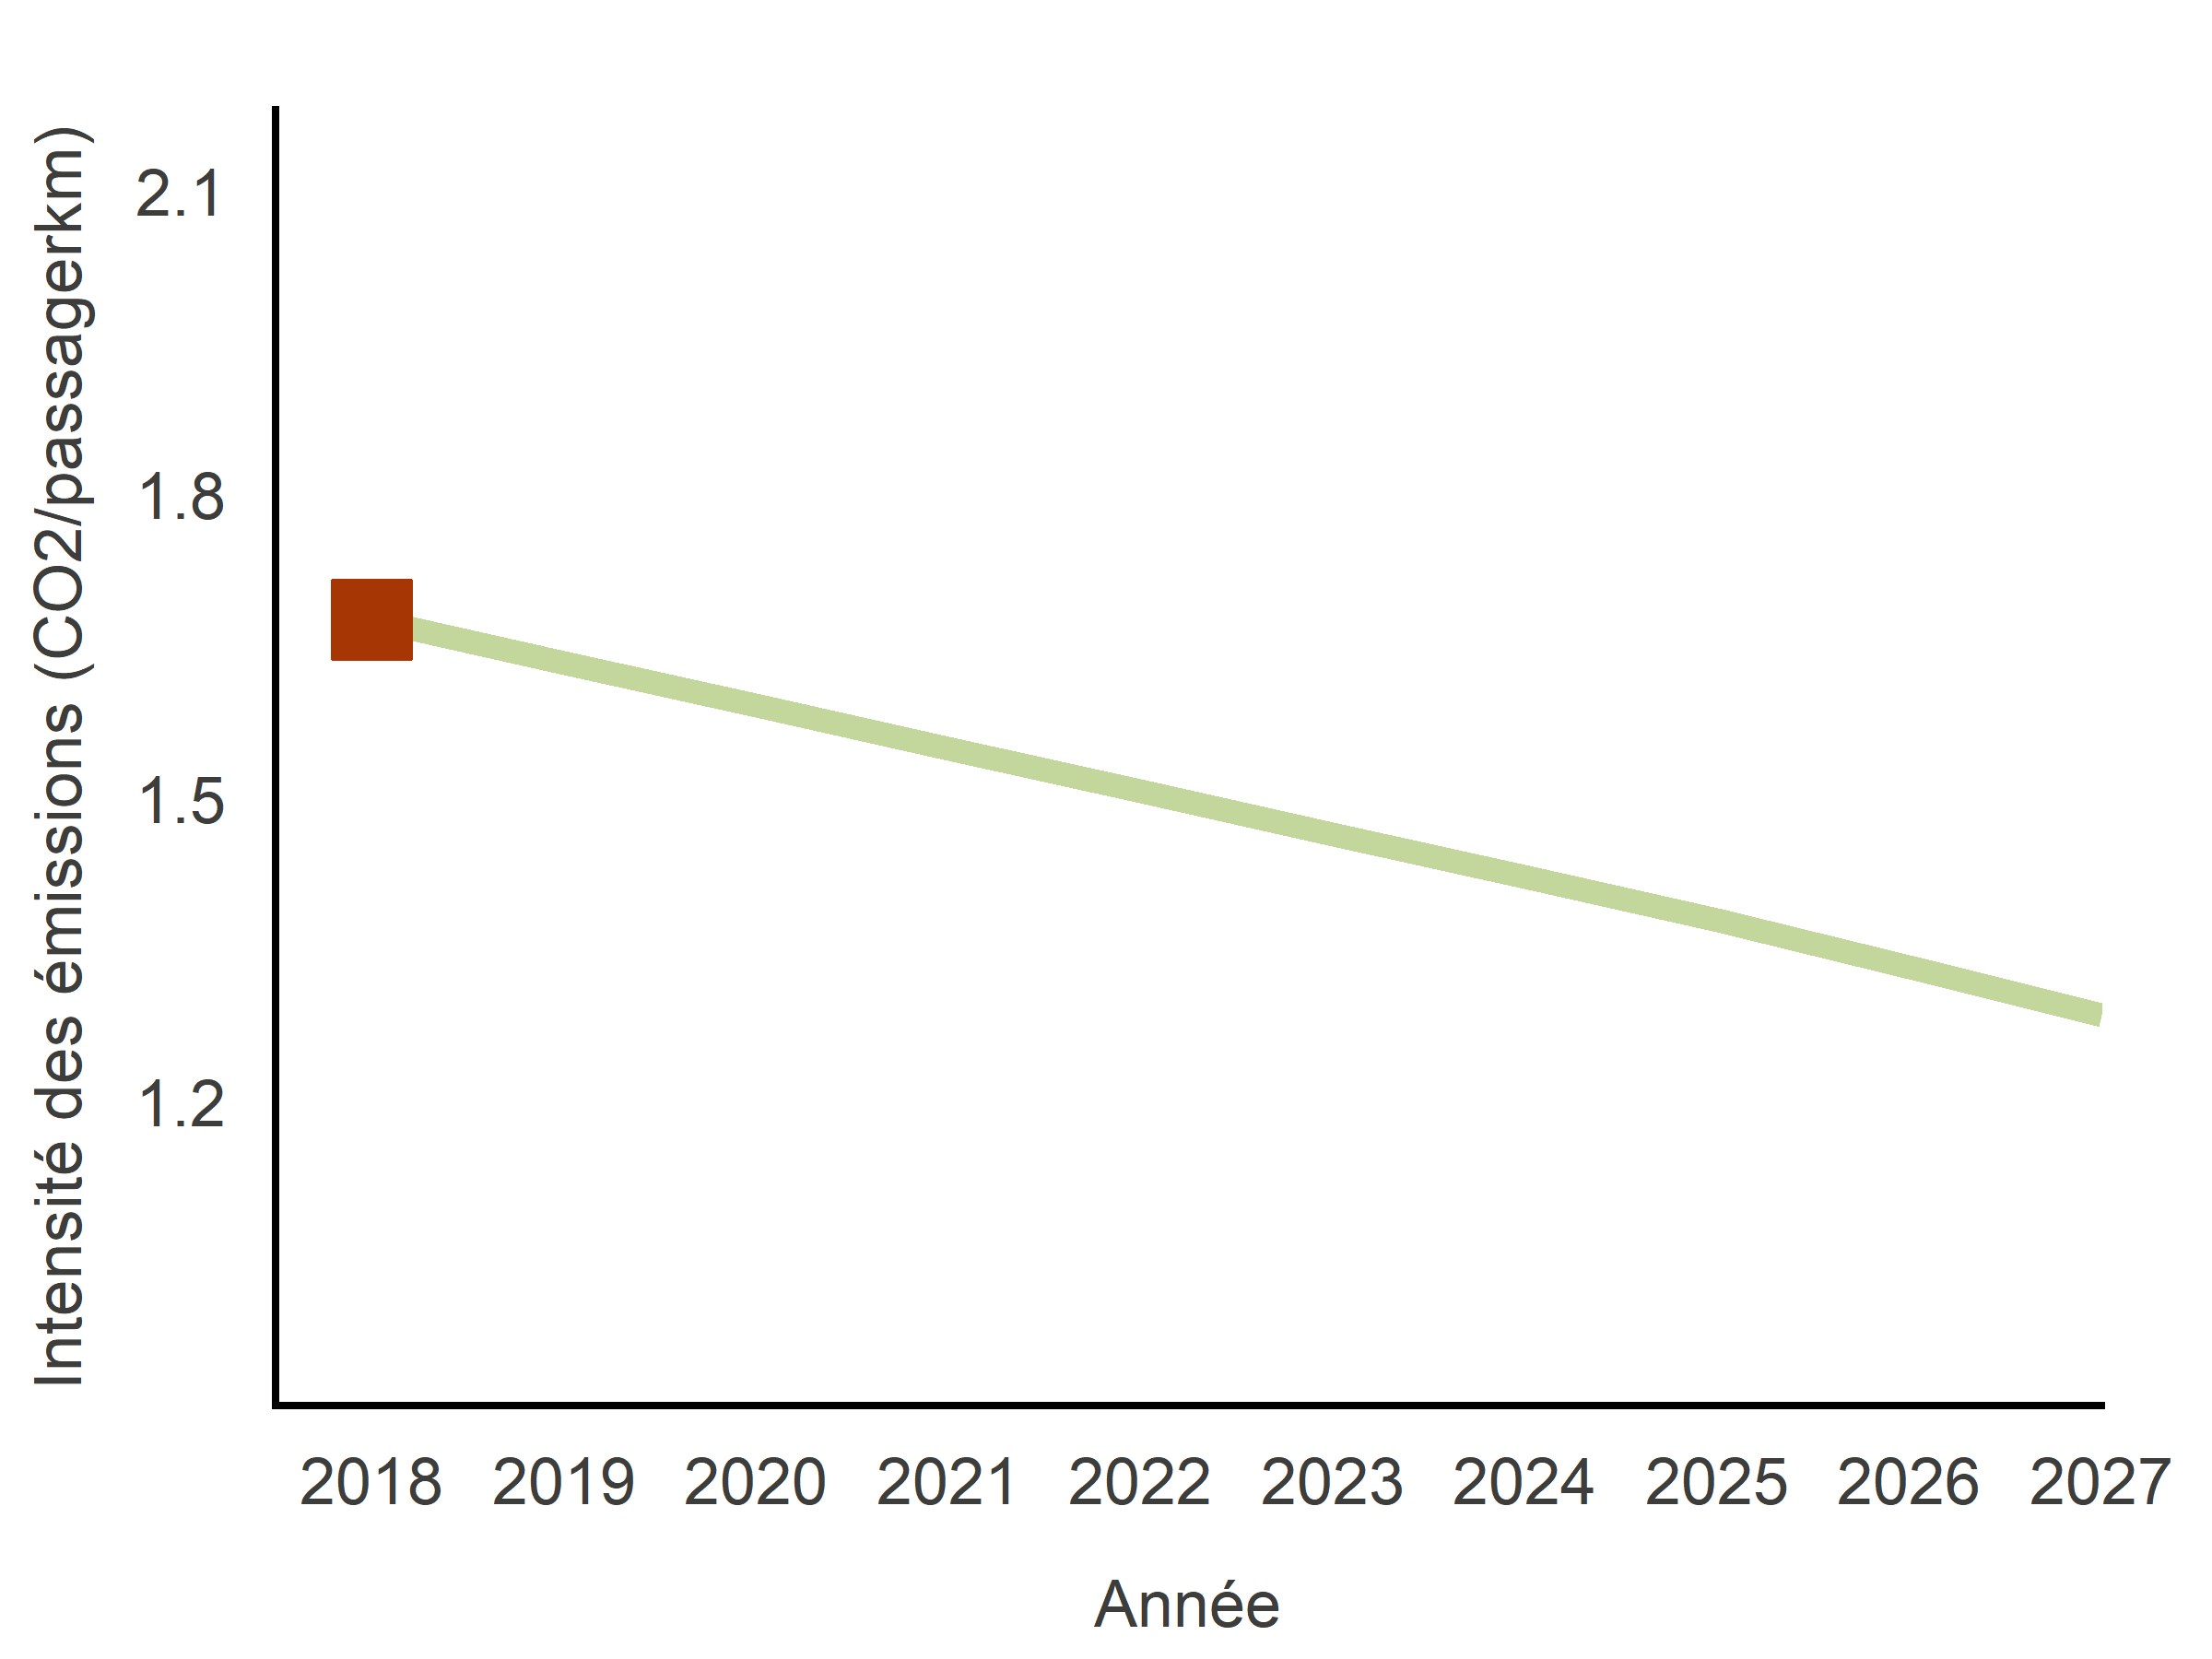
\includegraphics[trim = {0 0 0 0pt}, width=.9\linewidth]{ReportOutputs/Fig32}  \vfill\null \columnbreak
		
		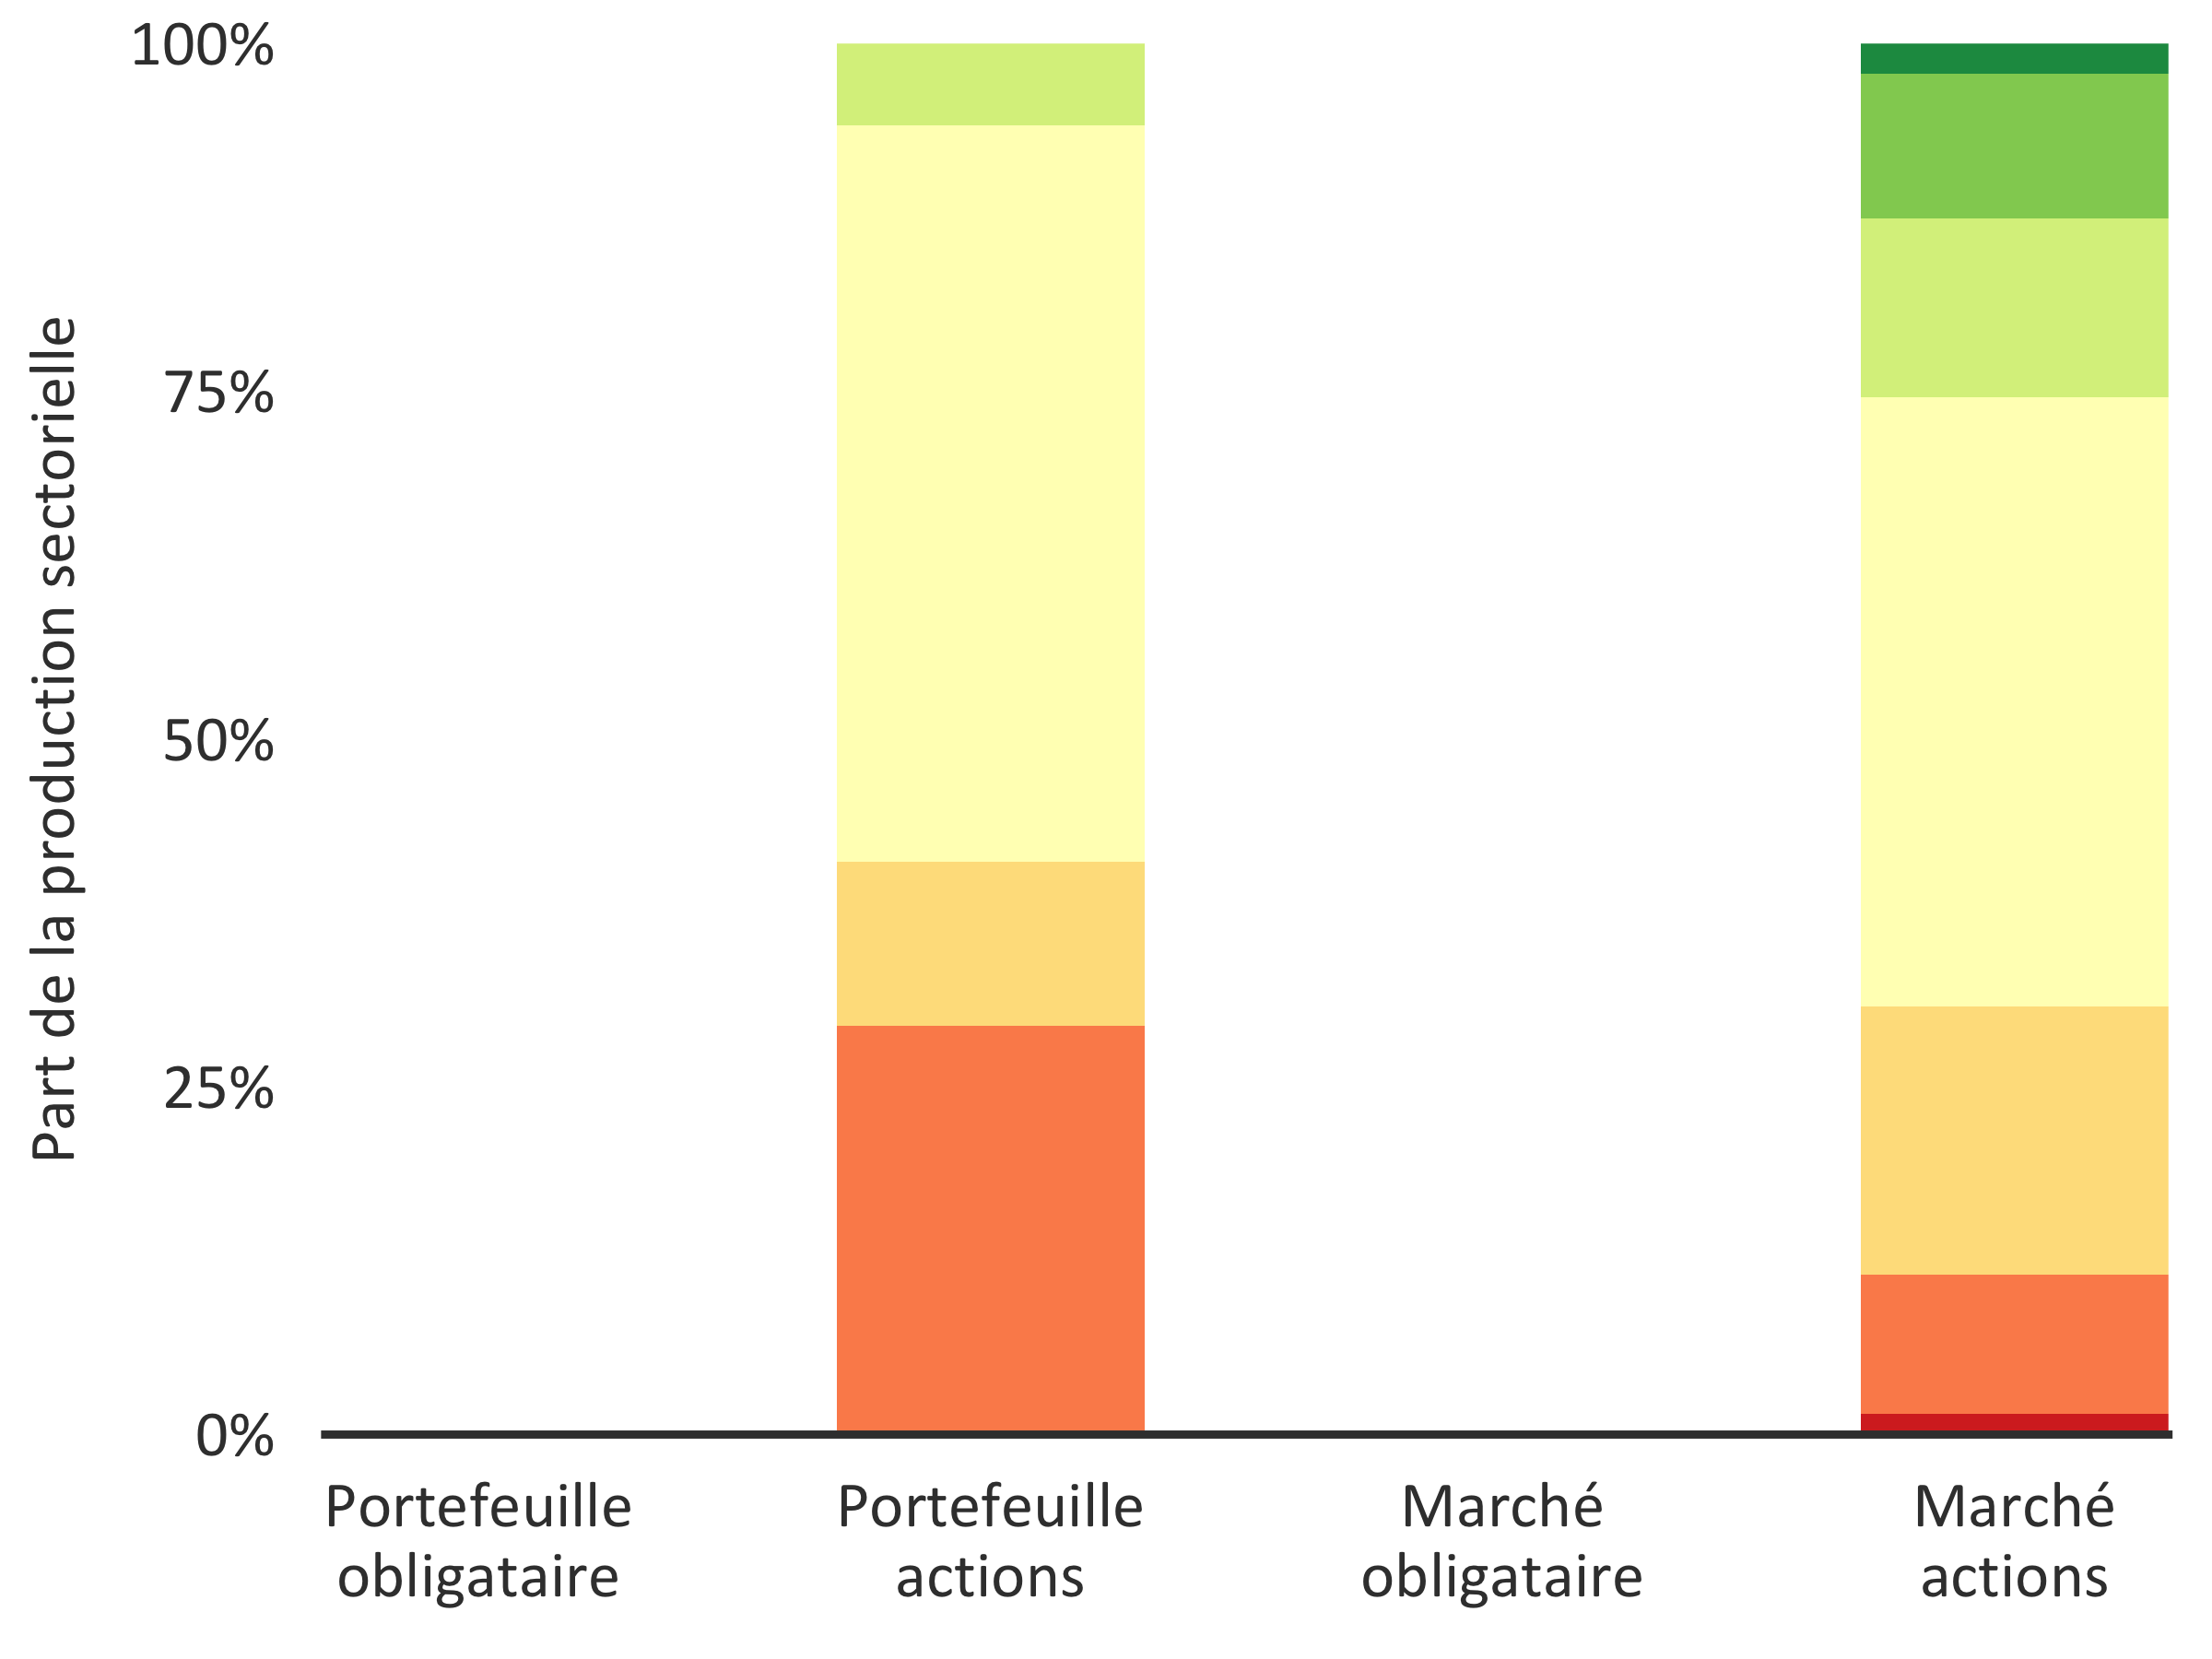
\includegraphics[width=1\linewidth]{ReportOutputs/Fig33}
		
	\end{multicols}
	
	\vspace{0pt}
	\setlength\multicolsep{0pt}
	
	\begin{multicols}{2}
		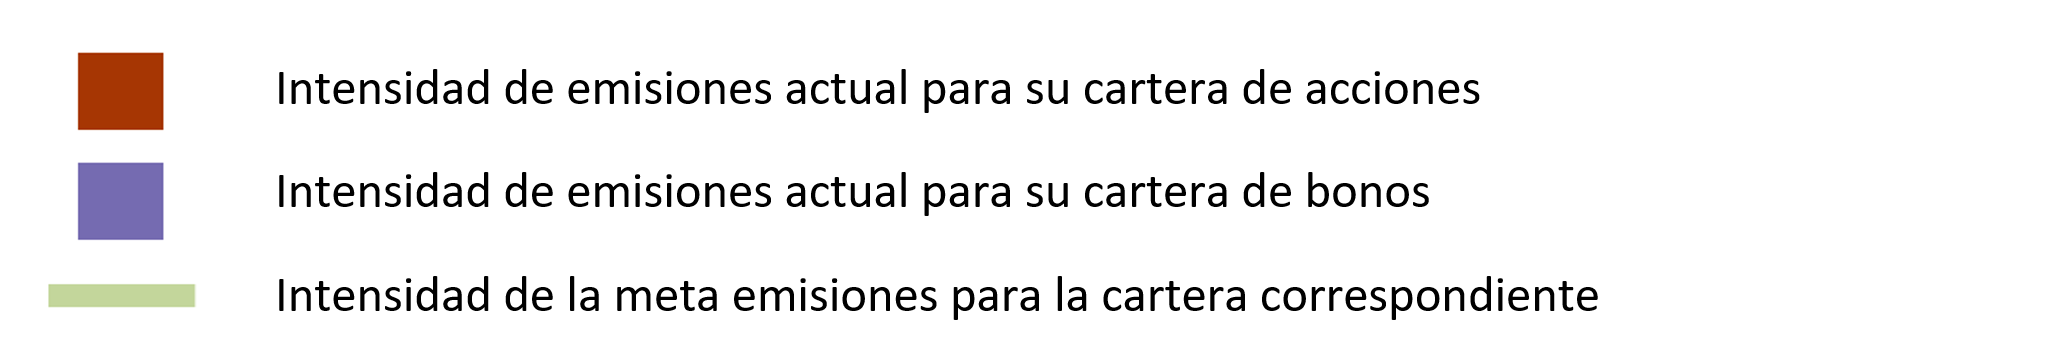
\includegraphics[width=1\linewidth]{ReportGraphics/OtherSectorLegend_ES}
		
		
		%NoShippingS
		\begin{center}
			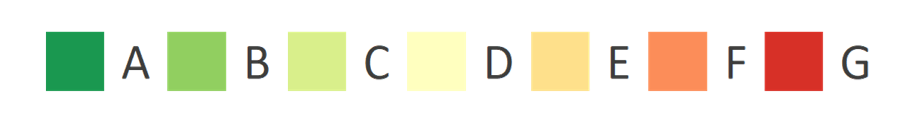
\includegraphics[width=0.6\linewidth]{ReportGraphics/ShippingLegend}
		\end{center}	
		%NoShippingE		
		
	\end{multicols}
	
	\textit{\small Fuente: 2Dii en base a EY 2016, PlantFacts, FlightAscend, Rightship, Carbon War Room, IEA 2017 and SDA 2015}
	
	\setlength\multicolsep{12pt}
	
	%\PageFooterThird 
\PageFooter{3 - TRAYECTORIA DE LA CARTERA}
	
	\newpage 
	% OtherSectorsE
	\section*{} % 4th SECTION 
	\SectionHeadingDouble{SECCIÓN 4:}{EXPOSICIÓN DE LA CARTERA  }{AL ScenarioValue EN Startyear+5}
	
	
	\newpage
	\section*{} % FUTURE TECHNOLOGY SHARE
	\HeaderSingle{PROPORCIÓN DE TECNOLOGÍA EN EL FUTURO}
	
	\begin{multicols}{2}
		\textbf{La siguiente grafica muestra la exposición estimada en Startyear+5 para las tecnologías de alto y bajo carbono en los sectores de combustibles fósiles, eléctricidad y automotriz tanto en las carteras de acciones como en la de bonos corporativos.}
		
		Los resultados son una función de ambos, el punto de partida de la exposición (sección 2) y de la evolución de la exposición a través del tiempo (sección 3), la cual es determinada en base a los planes de producción e inversión actualmente revelados por las empresas en la cartera. Los resultados muestran la exposición relativa de la cartera por clase de activo y tecnología/combustible. Los resultados son comparados con la combinación de tecnología/combustibles en un mercado alineado con un ScenarioValue en Startyear+5.
		
	Como se mencionó anteriormente, el análisis no incluye supuestos acerca de posibles cambios en la composición de las carteras. Al contrario, este análisis se limita a la variación en el tiempo de la exposición de la cartera a tecnologías de alto y bajo carbono en función de la evolución en la exposición de las empresas en la cartera. Los resultados ayudan a contextualizar la proporción de la exposición sectorial en expuesta a riesgos de transición en Startyear+5, considerando la proporción de actividades que pueden ser clasificadas como altas o bajas en carbono. Dada la naturaleza marginal de las actividades en energía renovable en las empresas de petróleo y gas, esta participación no ha sido considerada en el análisis, aunque con el tiempo esta puede representar una proporción creciente. 	
		
	\end{multicols}
	
	%CBSpecificS
	\textbf{Bonos Corporativos}
	
	
	\begin{center}
		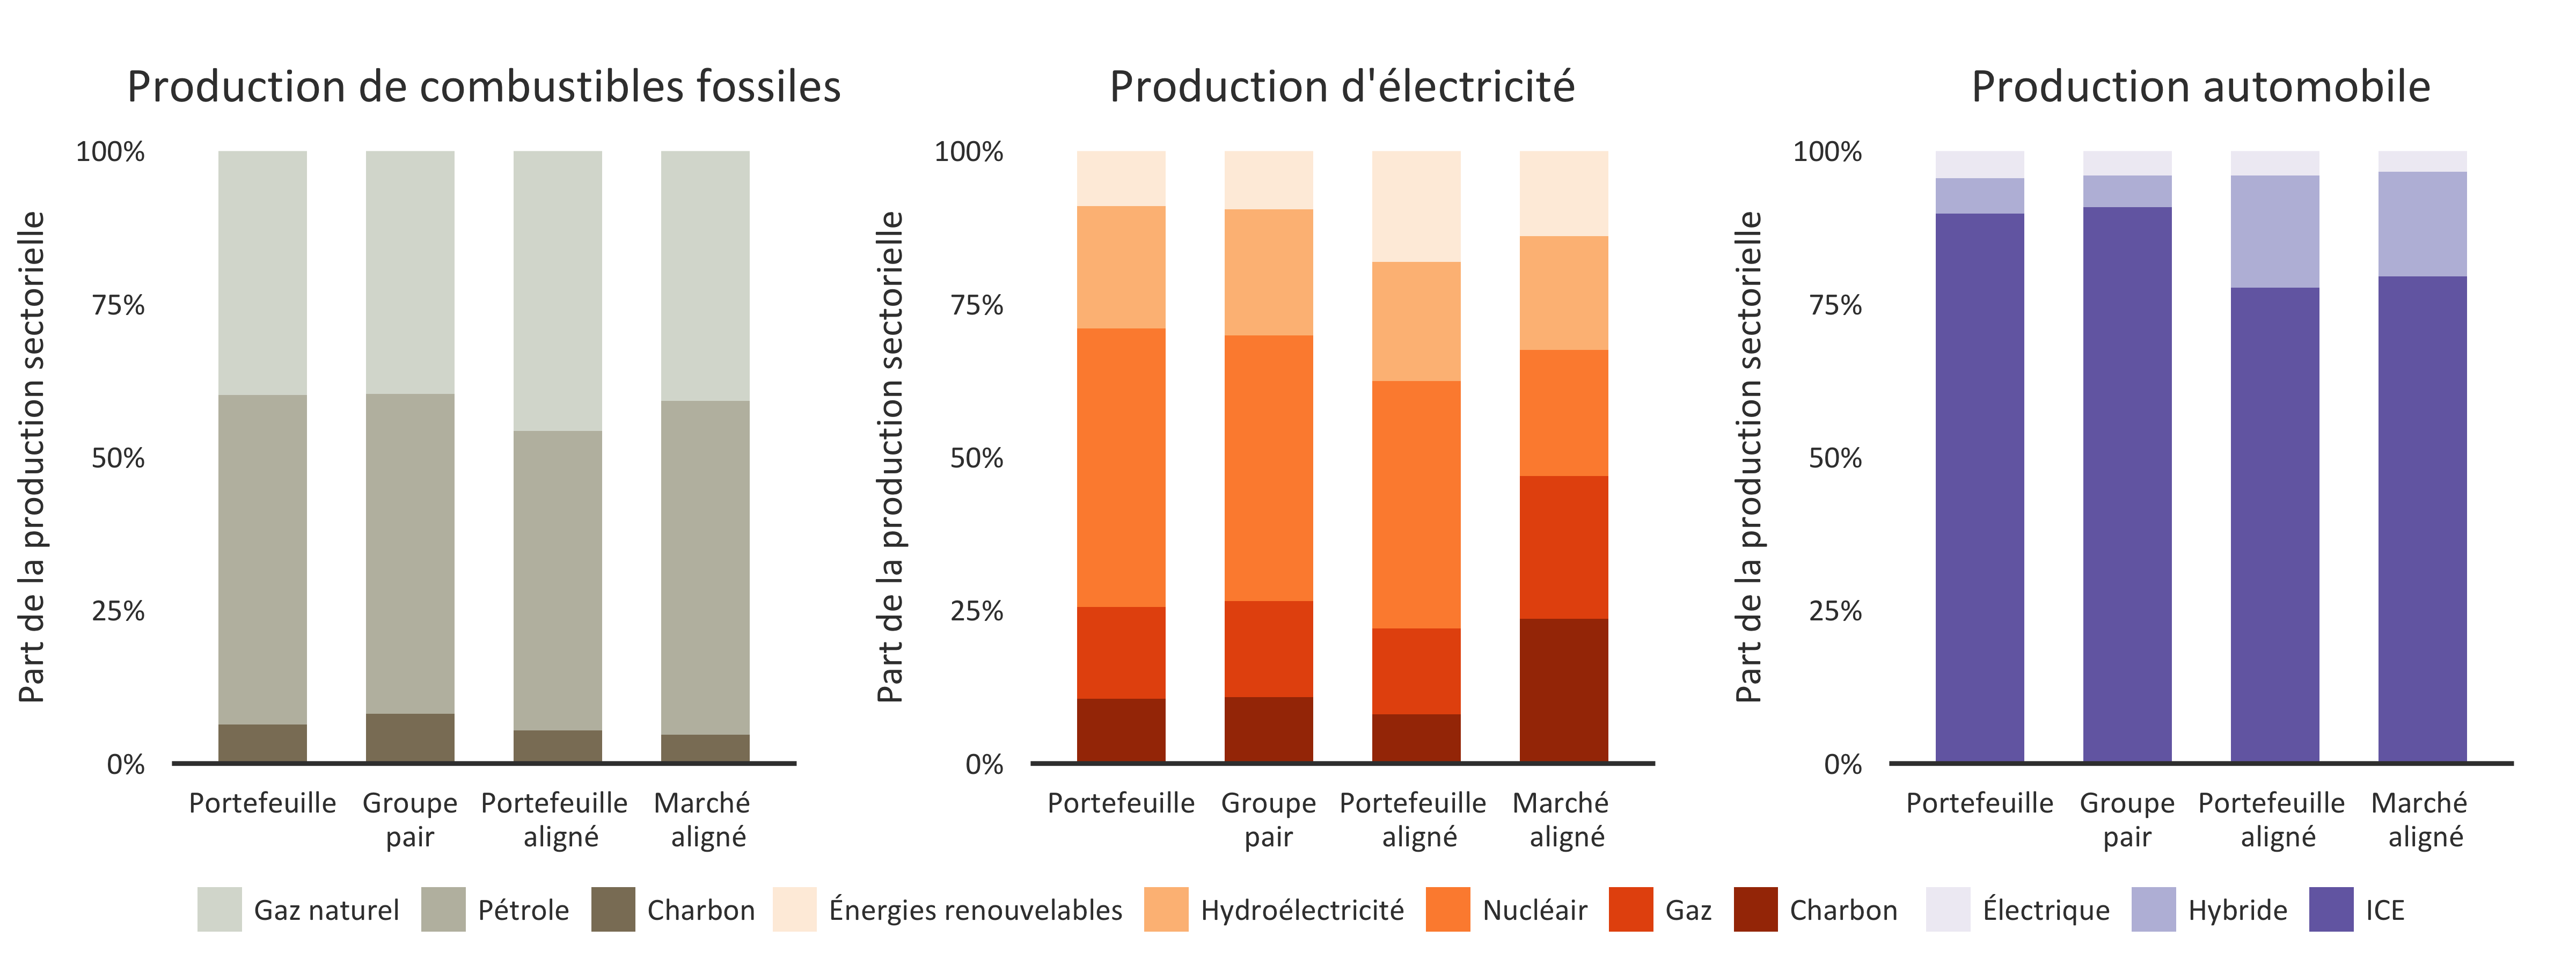
\includegraphics[trim = {0 0cm 0 0},width=1\linewidth]{ReportOutputs/Fig05}
	\end{center}
	%CBSpecificE	
	%EQSpecificS
	\textbf{Acciones}
	
	
	\begin{center}
		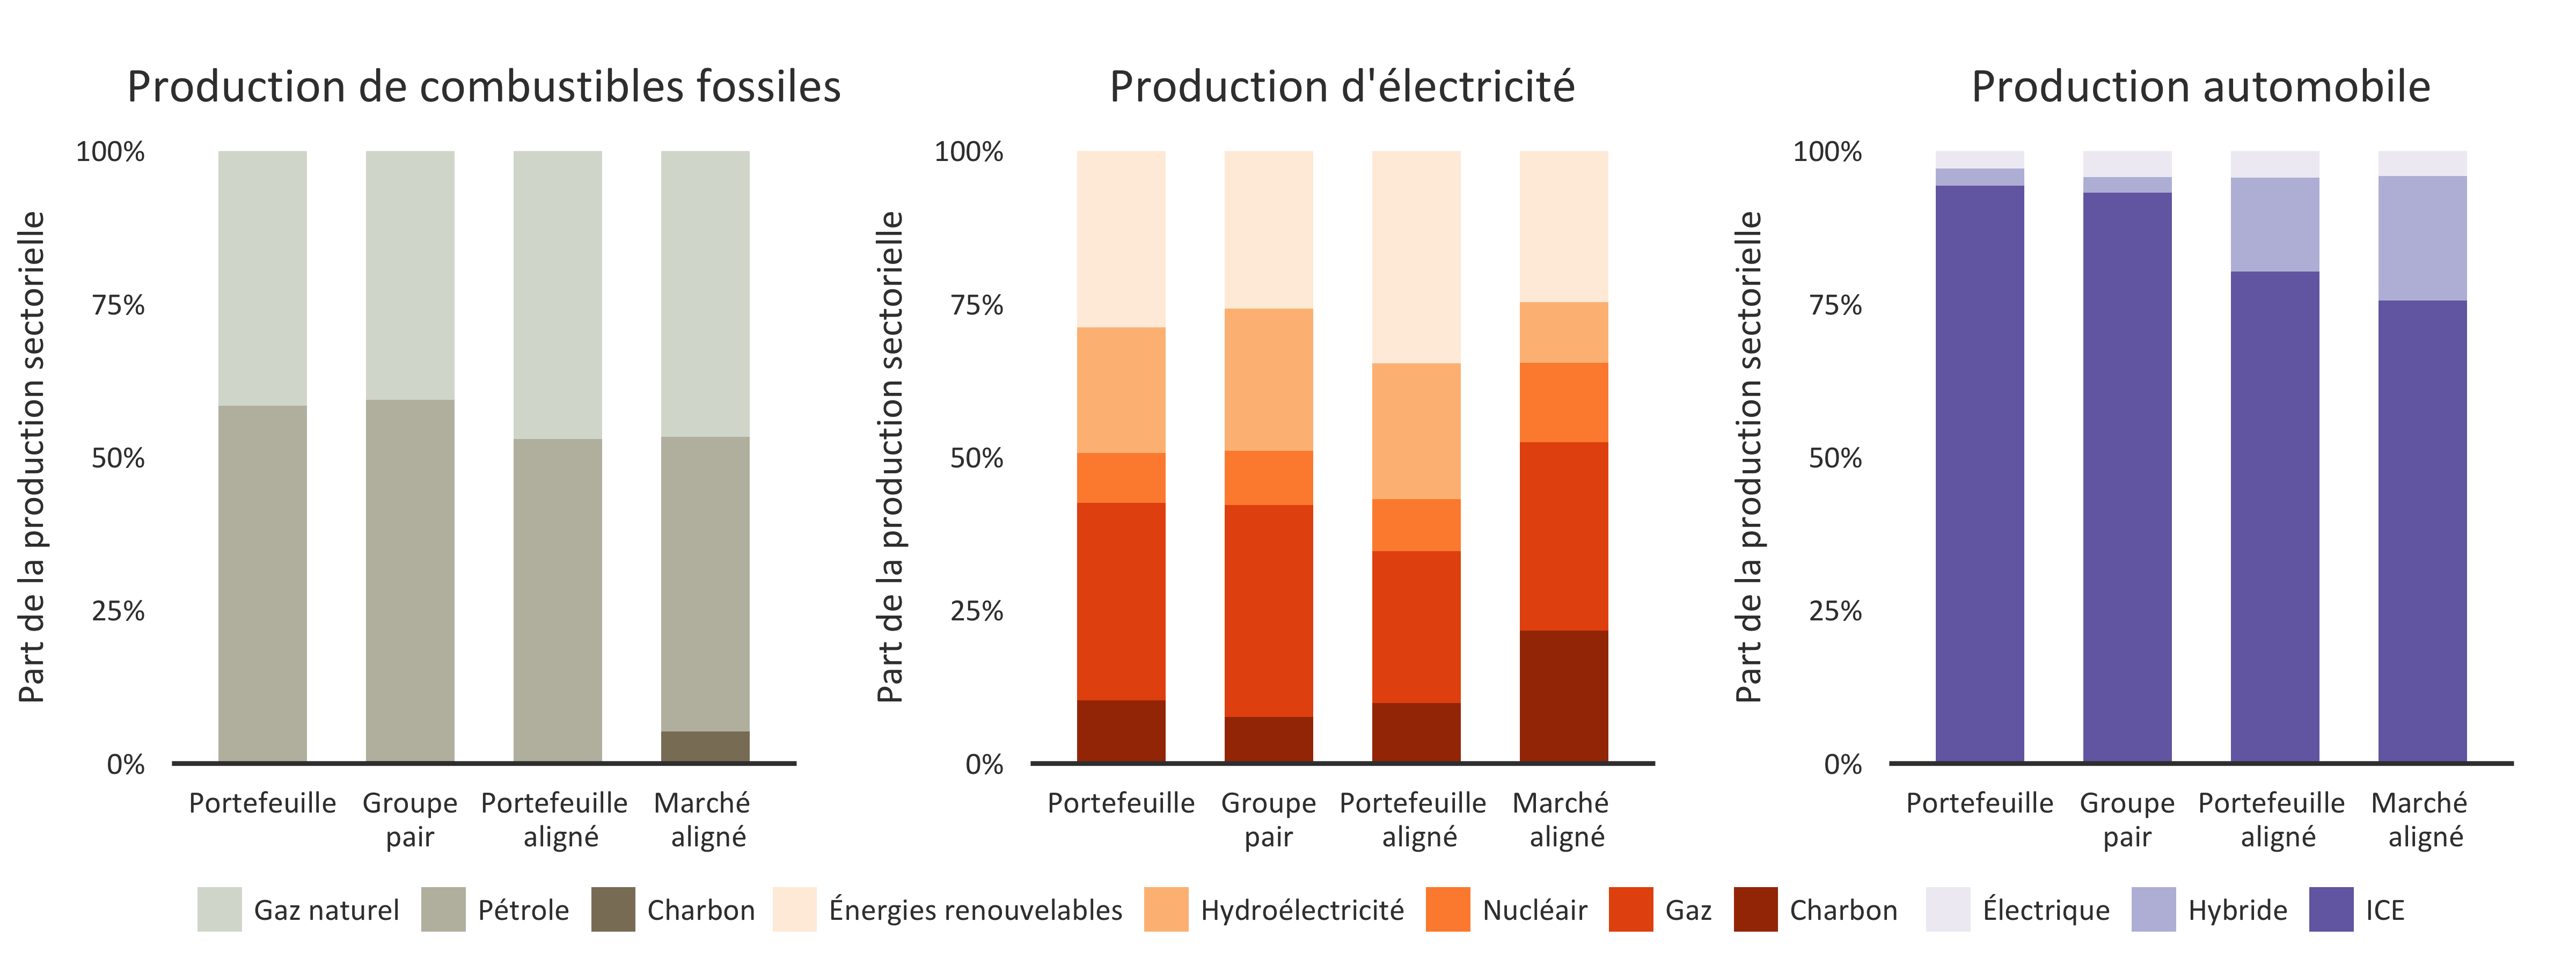
\includegraphics[trim = {0 0cm 0 0},width=1\linewidth]{ReportOutputs/Fig06}
	\end{center}
	%EQSpecificE
	%\PageFooterFourth
\PageFooter{4 - EXPOSICIÓN DE LA CARTERA }
	
	\newpage
	
	%CoalMiningChartS	
	\section*{} % REGIONAL EXPOSURE		
	\HeaderDouble{EXPOSICIÓN REGIONAL}{MINERÍA DE CARBÓN}
	
	\begin{multicols}{2}
		
	La siguiente grafica muestra la exposición regional de las carteras de bonos corporativos y acciones a la minería de carbón en Startyear+5.
		
		Esta es la suma de la minería de carbón asignada a la cartera en cada región.
		
	\end{multicols}	
	
	%CBSpecificS
	\textbf{Exposición regional de la cartera de bonos corporativos a la minería de carbón}
	\vspace{-.0cm}
	
	\begin{center}
		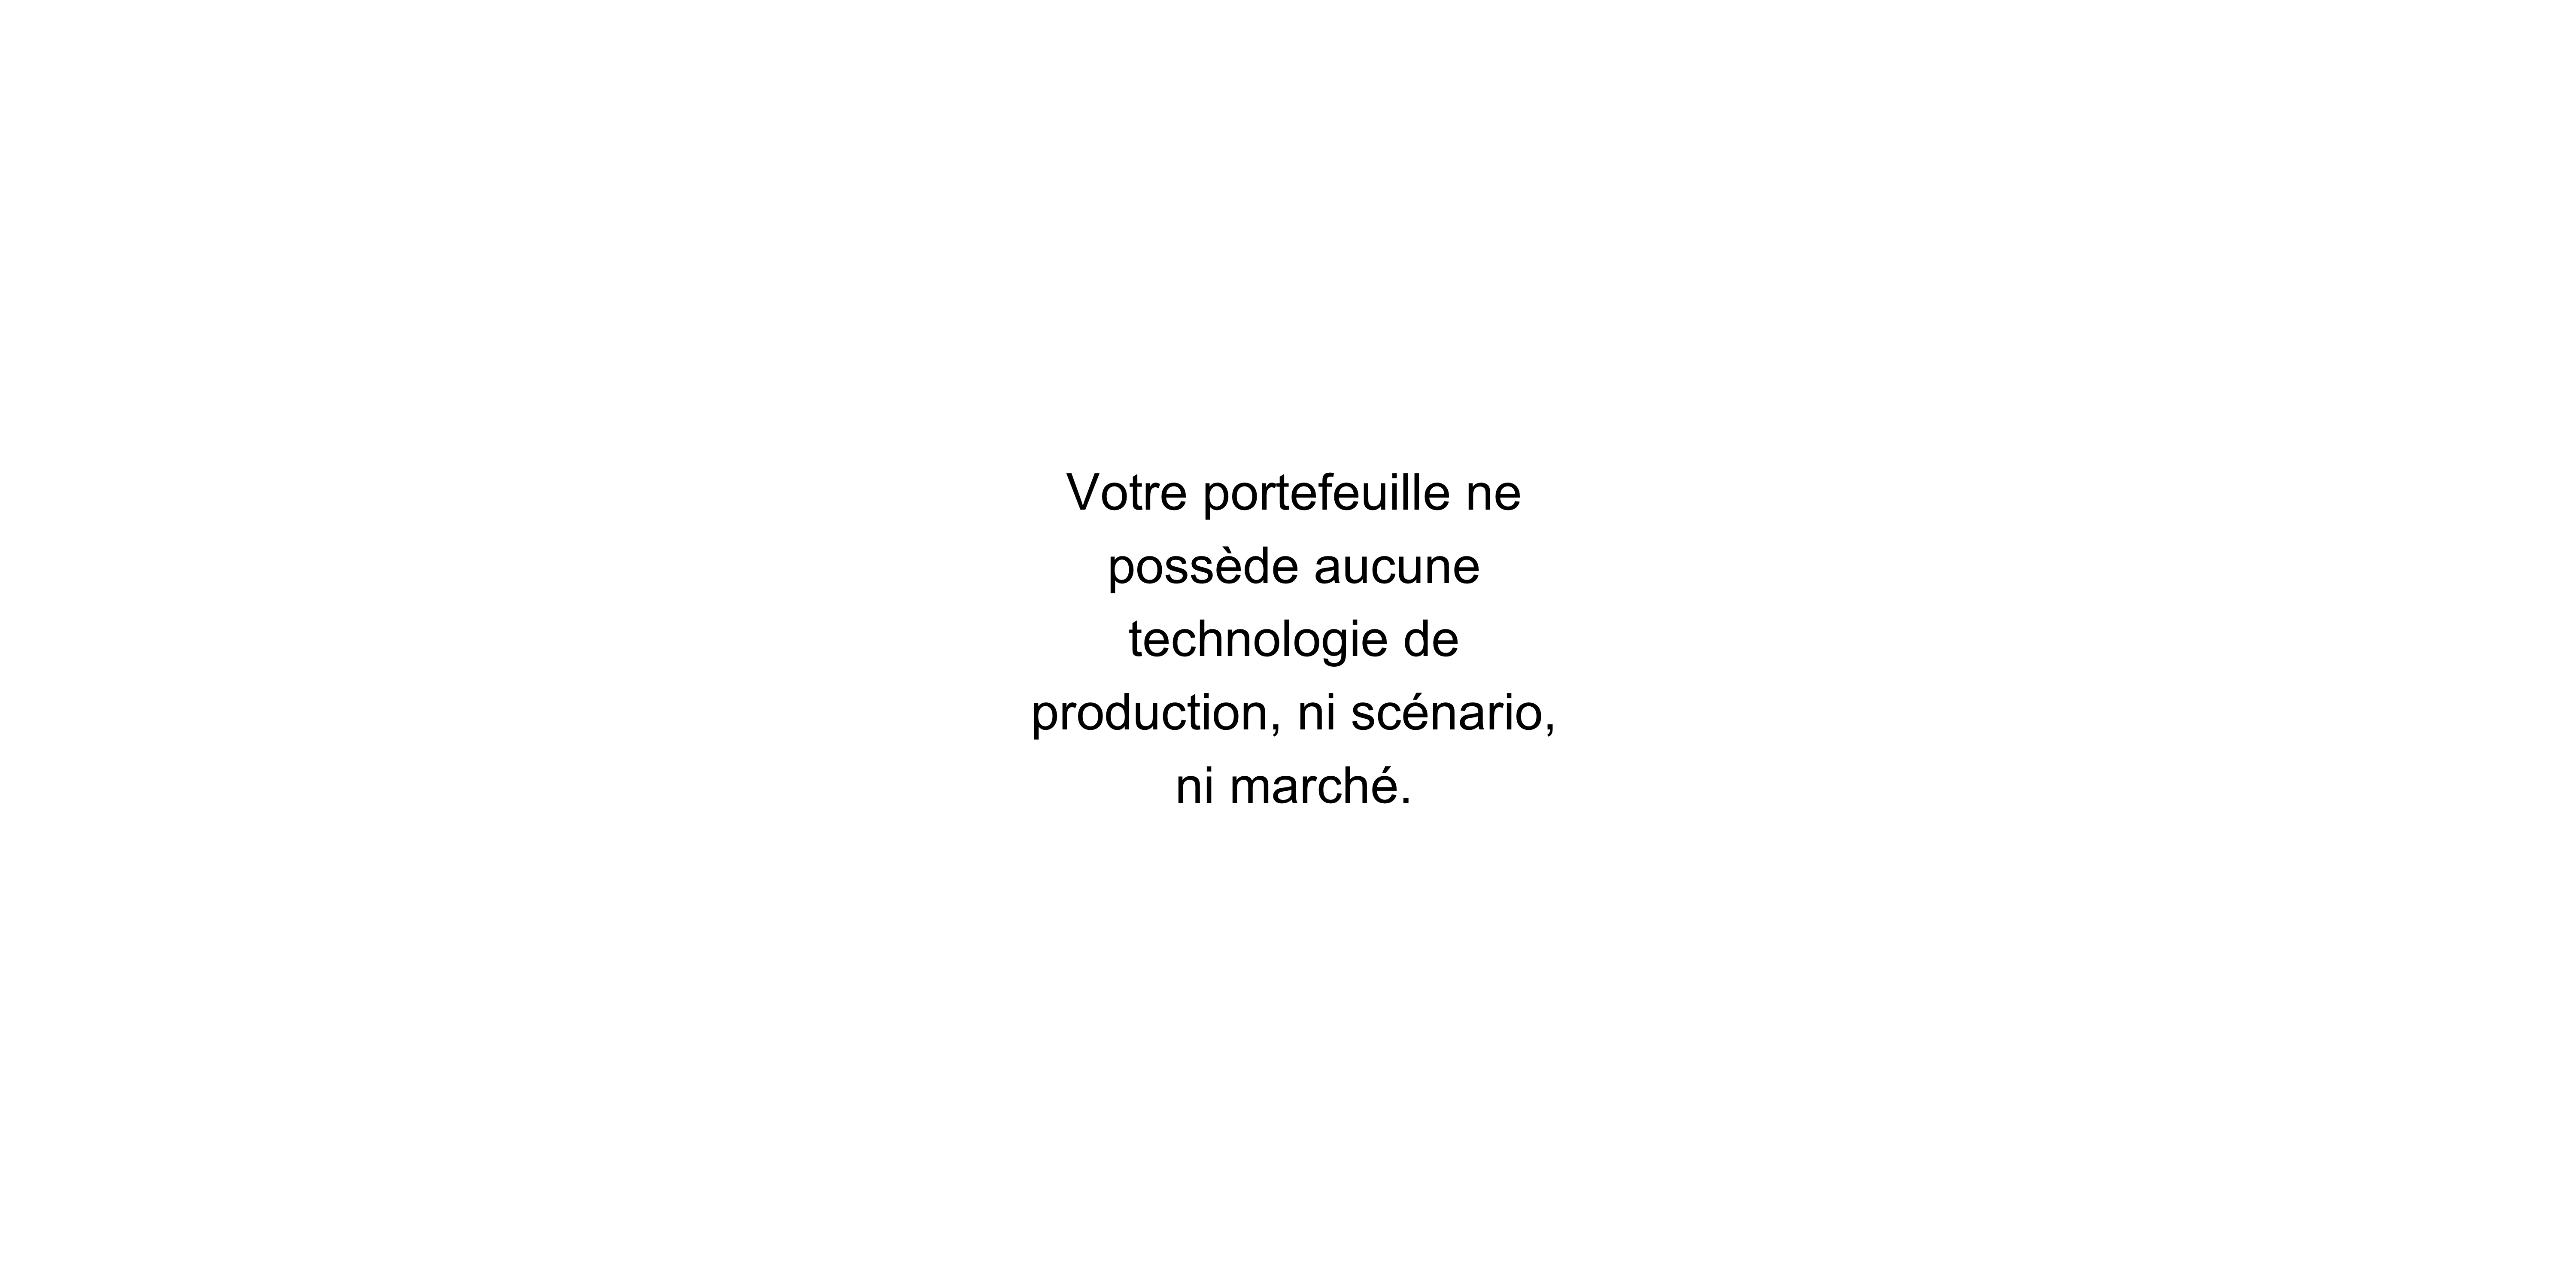
\includegraphics[trim = {2pt 2pt 2pt 2pt},clip,width=.9\linewidth]{ReportOutputs/Fig49}
	\end{center} 
	%CBSpecificE
	
	%EQSpecificS
	\textbf{Exposición regional de la cartera de acciones a la minería de carbón}
	\vspace{-.0cm}
	
	\begin{center}
		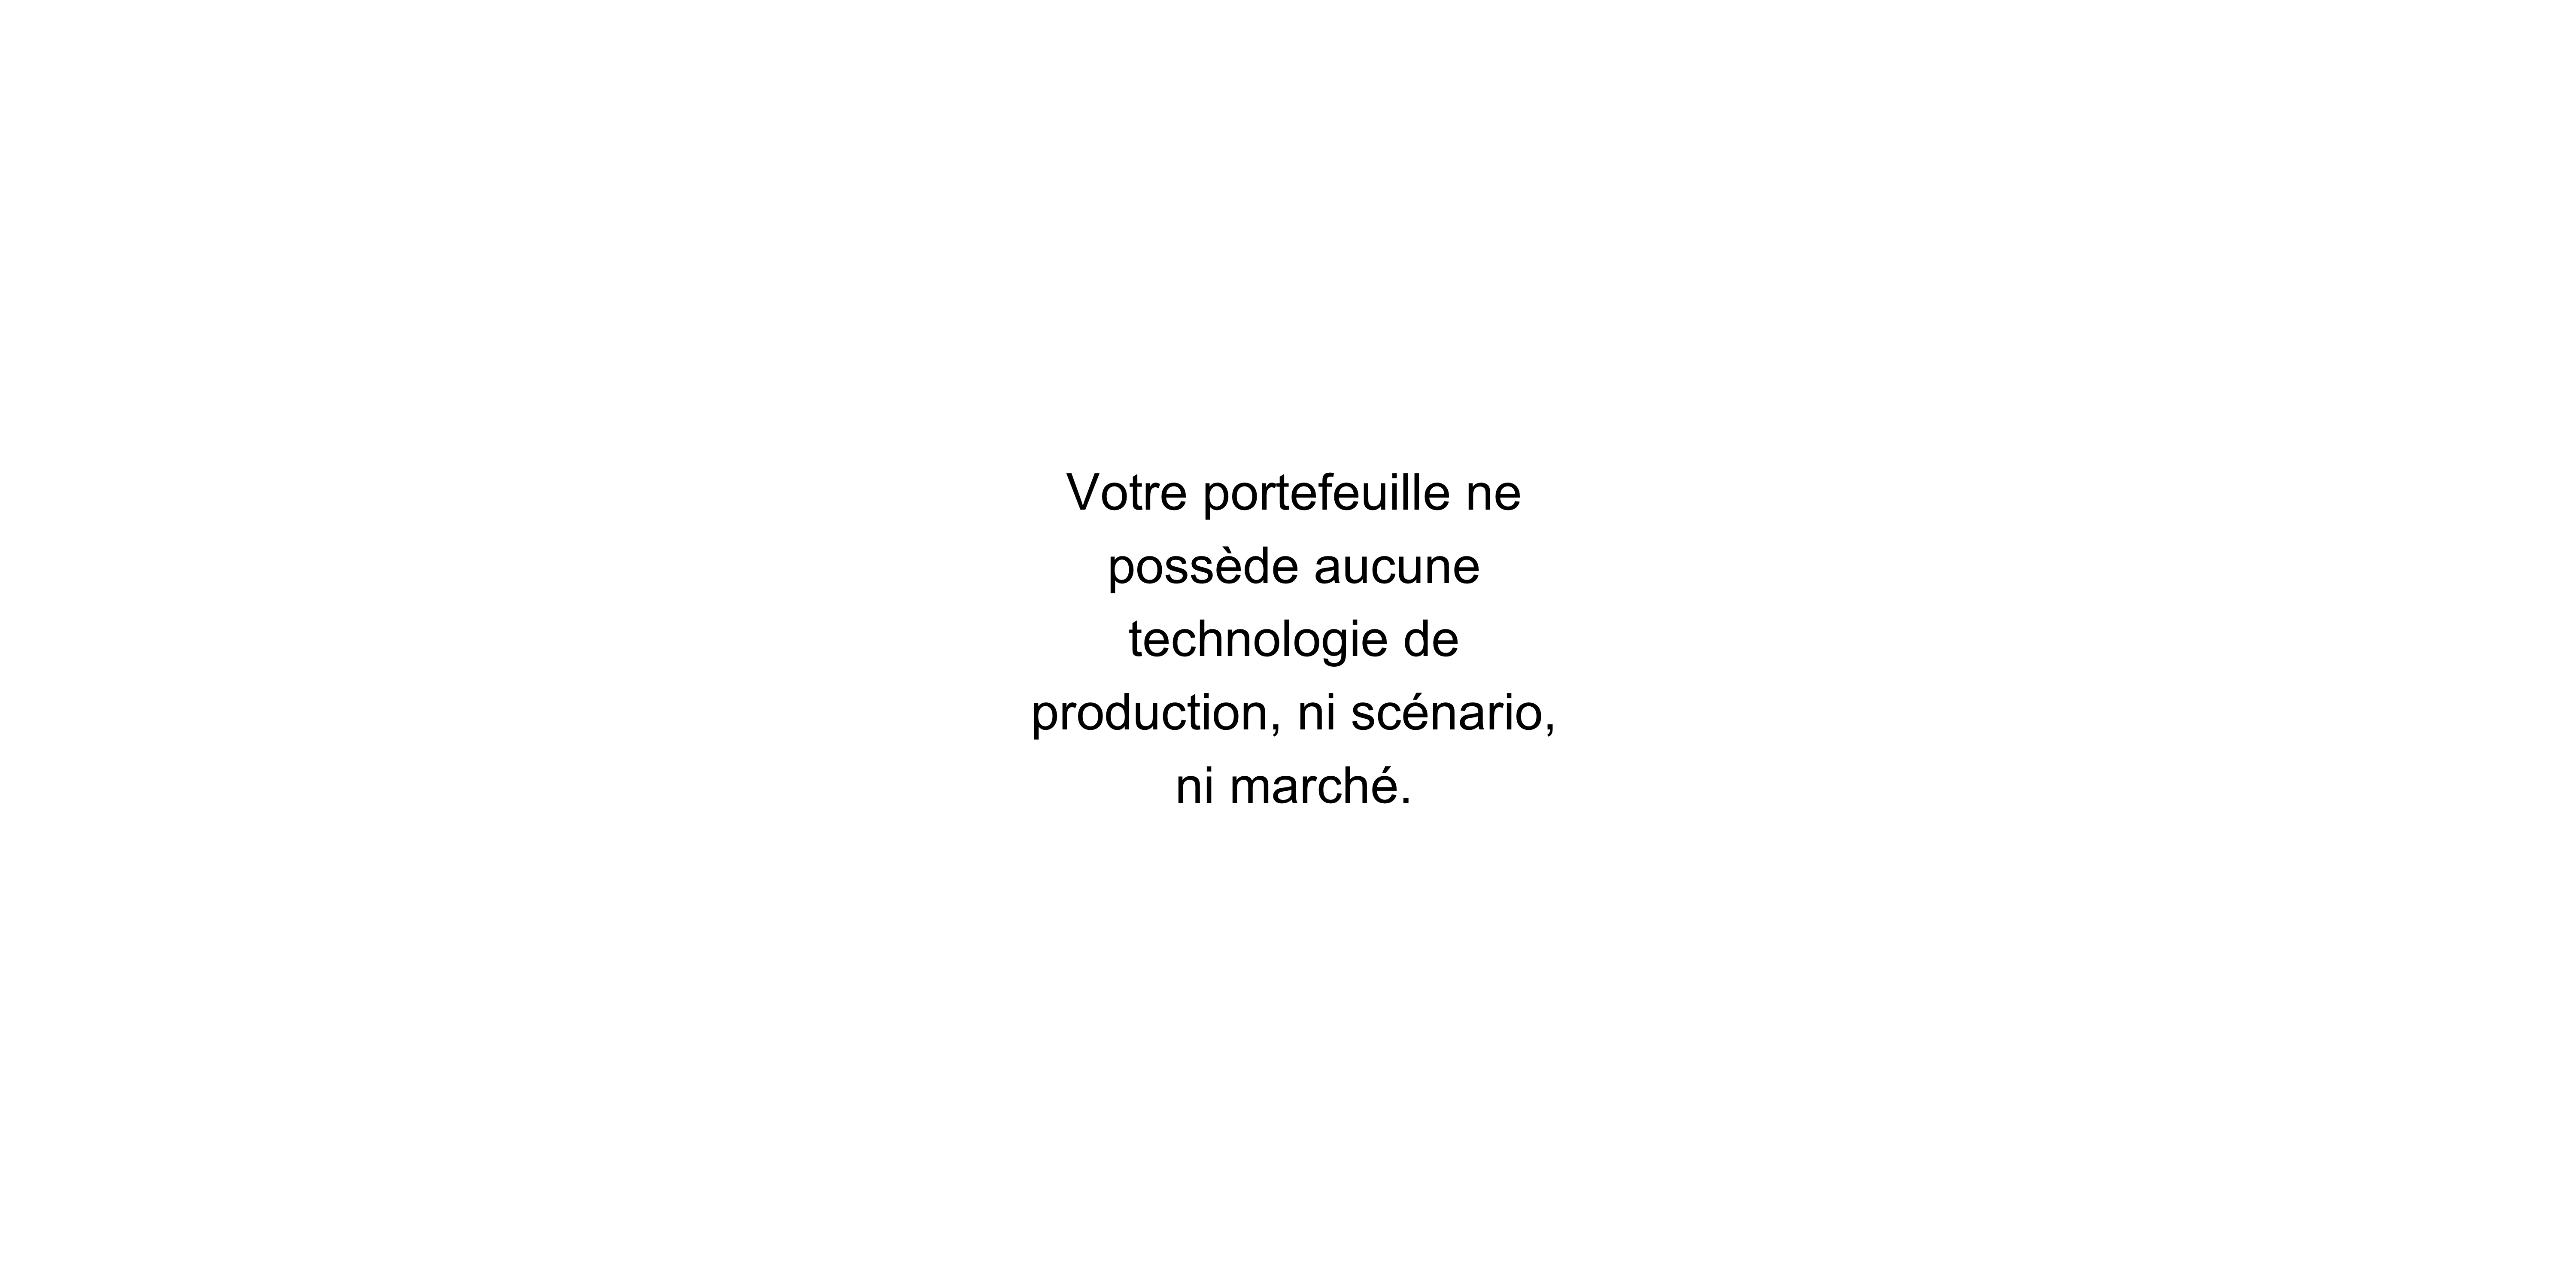
\includegraphics[trim = {1pt 1pt 1pt 1pt},width=.9\linewidth]{ReportOutputs/Fig50}
	\end{center} 
	%EQSpecificE
	
	%\PageFooterFourth
\PageFooter{4 - EXPOSICIÓN DE LA CARTERA}
	
	\newpage
	\section*{} % 5th SECTION   
	\SectionHeading{SECCIÓN 5}{EXPOSICIÓN DE LAS EMPRESAS}
	
	\newpage
	%CoalMiningChartE
	%CompanyChartsS
	\section*{} % CONTRIBUTIONS OF SECURITIES TO THE RESULTS 
	\HeaderSingle{CONTRIBUCIÓN DE LOS TÍTULOS FINANCIEROS A LOS RESULTADOS}
	
	\begin{multicols}{2}
		
		\textbf{El objetivo de esta sección es proporcionar información sobre las empresas que condujeron a los resultados presentados en las secciones anteriores.}
		
	Las siguientes páginas muestran los resultados por empresa en los sectores de combustibles fósiles, eléctrico y automotriz. El análisis proporcionado muestra solo información relacionada con un tipo análisis de escenario de empresas potencial y su contribución al desempeño de la cartera. Se podría considerar una gran variedad de indicadores adicionales que van más allá del alcance de este reporte. Los indicadores presentados en esta sección no deben ser considerados como recomendaciones de inversión, sino más bien como información sobre las empresas que conducen a los resultados del análisis de escenarios de cartera. La sección 7 proporciona más detalles de las fuentes de información que utilizan esta sección.
		
		2Dii en conjunto con varios expertos técnicos está desarrollando un reporte de análisis de escenario para empresas que replica el reporte de cartera presentado aquí. Este reporte estará disponible gratuitamente y proporcionará una imagen más completa y holística del posicionamiento de una empresa en relación con escenarios de decarbonización. El reporte podrá ser usado para informar el análisis de escenarios y las acciones climáticas a futuro y será lanzado en el cuarto semestre de 2019. Por lo tanto, el análisis de este reporte solo muestra una fotografía instantánea del tipo de datos que se pueden explorar.
		
	A continuación, se resumirá brevemente el tipo de información que se mostrará para cada sector presente en la cartera. 
		
		\textbf{Sector de petróleo y gas: }Para la producción de petróleo y gas se muestran tres tipos de indicadores.
		
		
		\begin{enumerate}
			\item {	El primer indicador muestra el cambio total previsto en la producción de empresas petroleras en los próximos 5 años. Este indicador se basa en los planes de producción revelados de las bases de datos de activos físicos. Los gráficos de la siguiente página muestran las empresas petroleras con más participación en la cartera de acciones y bonos en Startyear. Estas empresas son las que tienen más influencia en los resultados de alineación de la cartera en el sector de combustibles fósiles. Para cada clase de activo y tecnología, los resultados se muestran en relación con el cambio total en la producción de la cartera según el ScenarioValue (barra verde) en los próximos 5 años. Cabe señalar que las cifras proporcionadas se basan en estimaciones actuales de la producción y la evolución de la base de activos físicos existentes.
			Las fusiones, adquisiciones y aumentos en gastos de capital pueden llevar a cambios en estas tendencias a lo largo del tiempo. }
			\item {	El segundo indicador se apoya en el análisis realizado por Carbon Tracker Initiative en colaboración con los Principios para la Inversión Responsable de las Naciones Unidas (UNPRI por sus siglas en ingles). Este indicador adopta una visión a largo plazo y analiza la alineación de las empresas a un presupuesto de carbono de 2\degree C considerando la estructura de costos de sus activos de petróleo y gas. Este indicador difiere con el primero en el horizonte temporal y las reglas de asignación subyacentes que asignan escenarios macroeconómicos a actores microeconómicos. Más información sobre la metodología y su enfoque se puede encontrar en http://www.2degreeseparation.com/. Este indicador puede ser utilizado solamente para analizar la cartera de acciones ya que la data no está disponible para bonos corporativos.}
			\item 	{El tercer indicador muestra el desglose de los activos petroleros por empresa para cada tipo de hidrocarburo (e.g. petróleo convencional, arenas bituminosas, etc.). Wood Mackenzie (2018) propone que, aunque el desplazamiento de los combustibles con alto contenido de carbono hacia los bajos en carbono es necesario como una tendencia general, dentro de la industria del petróleo y el gas, el cambio en ciertos métodos de extracción es una alternativa de transición. Este reporte no comenta sobre las emisiones por tipo de extracción, sin embargo, hay información disponible al respecto. Los inversionistas deben mirar más allá de los temas ligados a los recursos y examinar la variación de la intensidad de emisiones asociadas a procesos de producción y procesamiento para entender como las empresas pueden reducir su huella de carbono. Activos de un mismo tipo pueden incluso tener una intensidad de emisiones diferente debido a su madurez, localización y otros factores específicos del activo.}
		\end{enumerate}
			
		\textbf{Sector Eléctrico y automotriz.} Para el sector eléctrico y automotriz, la información a nivel de empresas se centra en la combinación de tecnologías de empresas generadoras de electricidad y los fabricantes de automóviles en las carteras de bonos corporativos y acciones, informando en particular los resultados de la sección 4. Información adicional sobre los planes de expansión de estas empresas y las variaciones a lo largo del tiempo puede ser suministrada a petición.
		
		%CBSpecificS
		\textit{Favor notar que para la cartera de bonos los resultados son suministrados a nivel de ticker de deuda. Esto debido a que un ticker de deuda puede estar asociado con múltiples empresas.}
		%CBSpecificE
		
	\end{multicols}
	
	%\PageFooterFifth
\PageFooter{5 - EXPOSICIÓN DE LAS EMPRESAS}
	
	\newpage
	%FossilFuelSector_ALLS
	%FossilFuelSector_CBS
		\section*{} % CONTRIBUTIONS OF SECURITIES TO THE RESULTS 
	\HeaderDouble{CONTRIBUCIÓN DE LOS TÍTULOS FINANCIEROS A LOS RESULTADOS}{PETRÓLEO Y GAS – BONOS CORPORATIVOS} 
	
	
	

	
	\vspace{-.05cm}
	\textbf{Cambios previstos en la producción de petróleo y gas de las empresas con mayor participación en la cartera de bonos corporativos en Startyear+5.} Esta gráfica muestra el aumento o disminución previsto en la producción en los 5 próximos años de gas y petróleo de las empresas más grandes del sector que se encuentran en la cartera de bonos corporativos. Este es comparado con los cambios requeridos según el ScenarioValue.
	\vspace{-.15cm}
	
	\begin{center}
		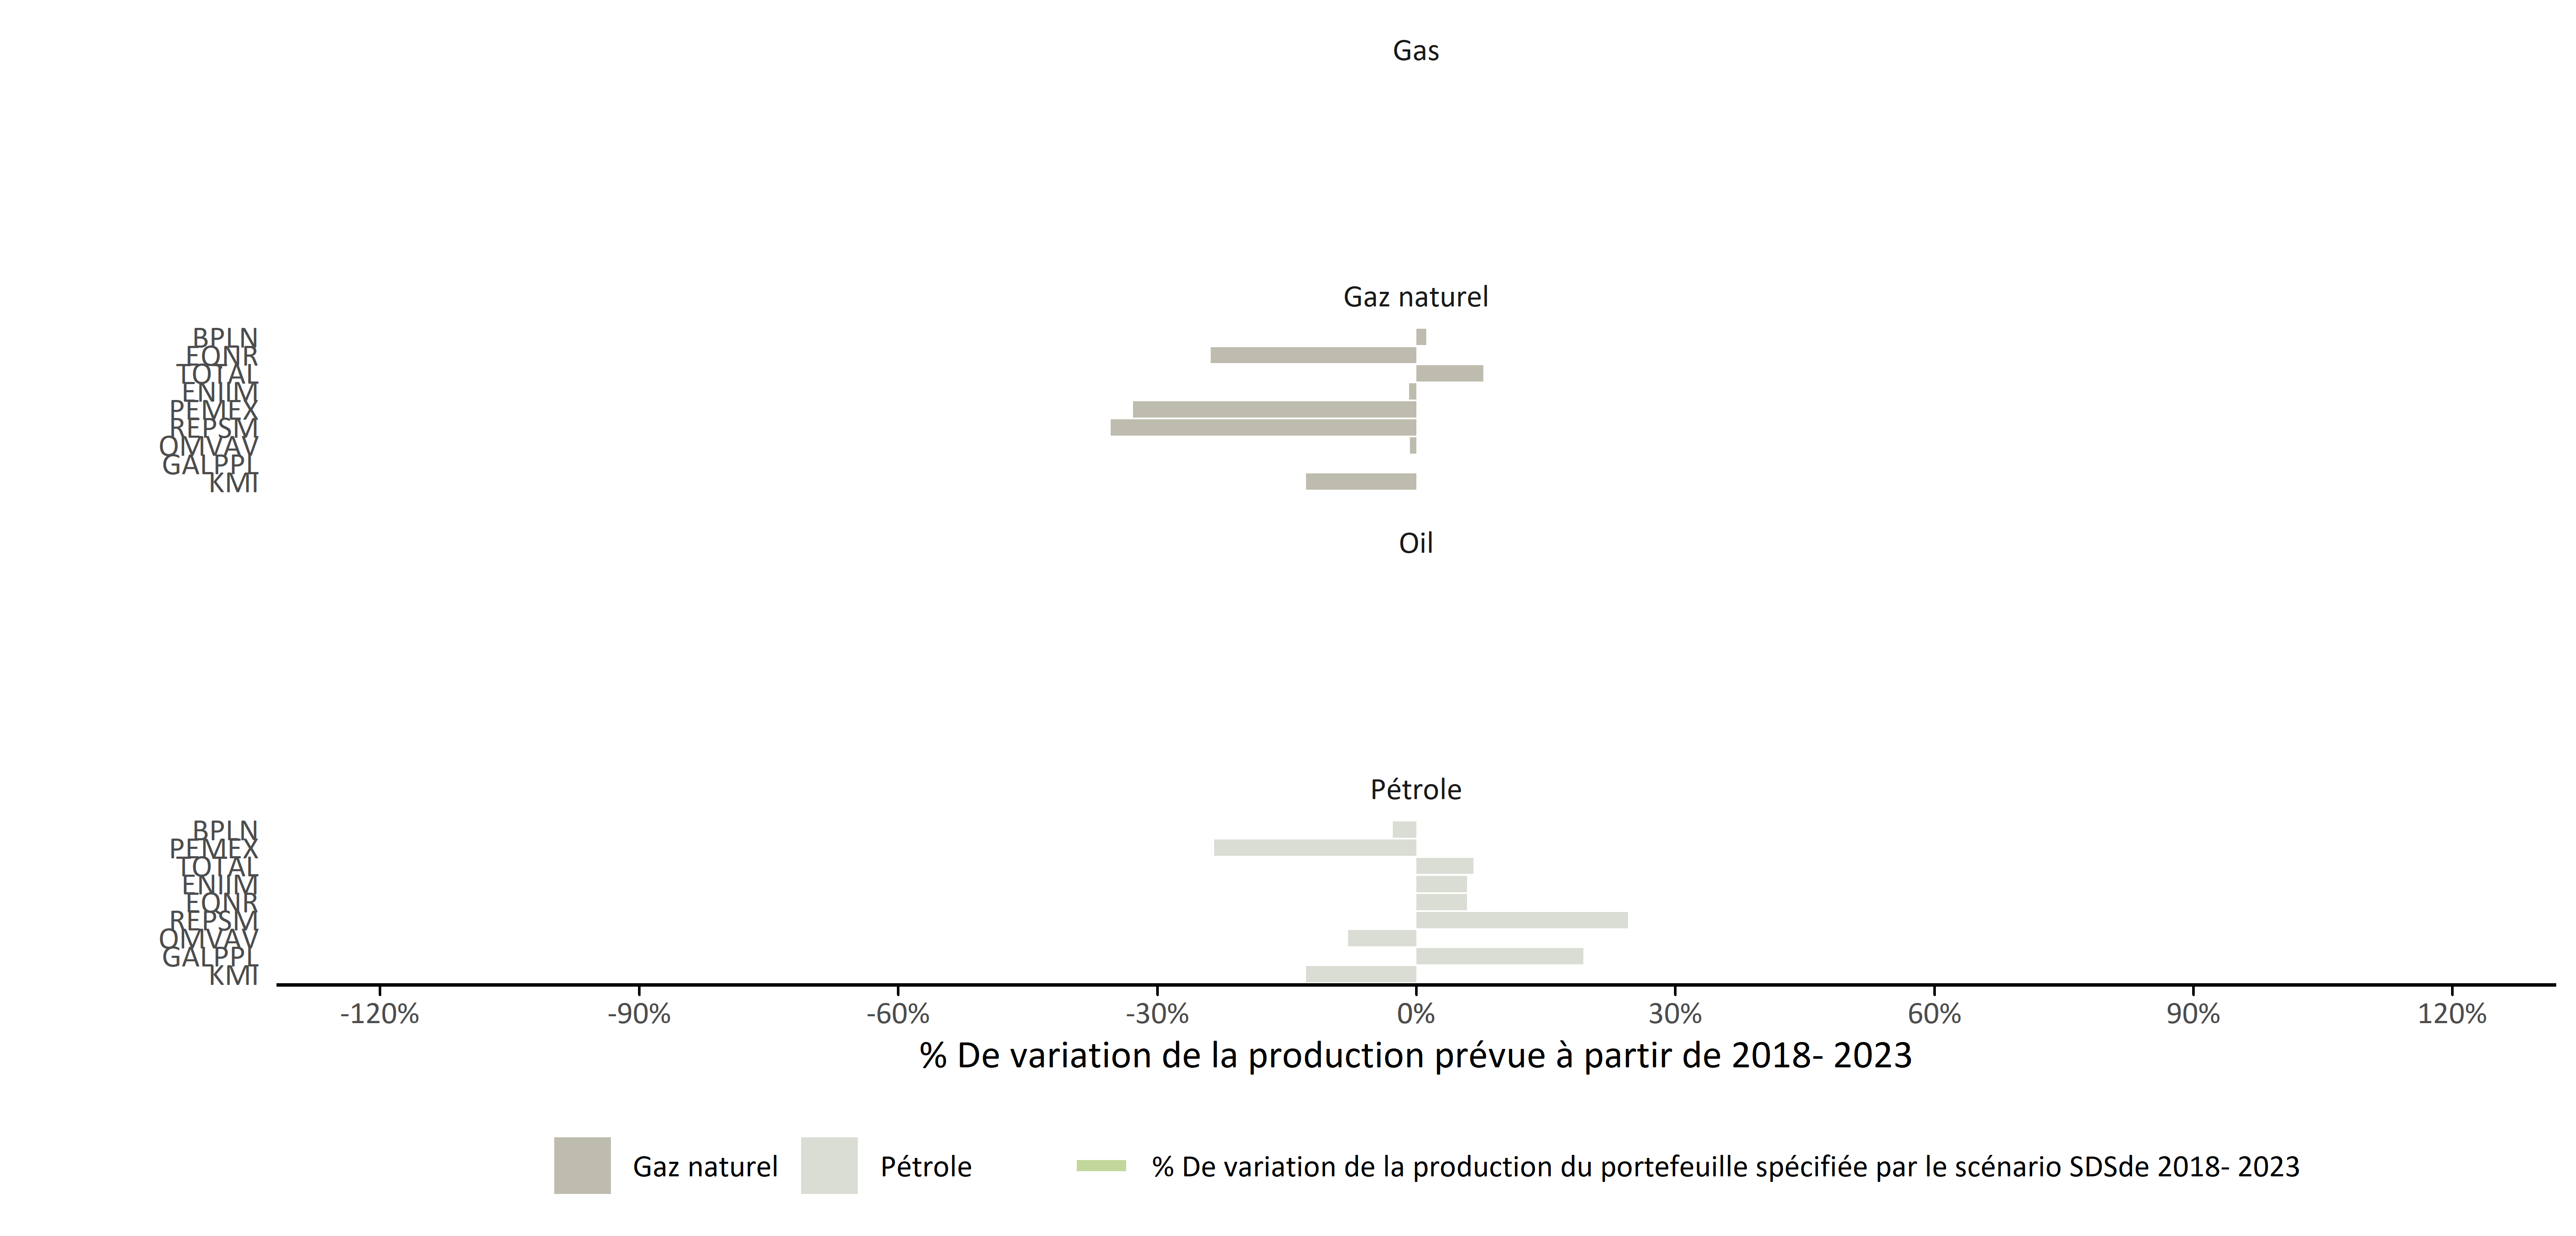
\includegraphics[trim = {0 0cm 0 0},width=1\linewidth]{ReportOutputs/Fig42}
	\end{center}

	\PageFooter{5 - EXPOSICIÓN DE LAS EMPRESAS}



\newpage

%FossilFuelSector_CBE
%FossilFuelSector_EQS
	\section*{} % CONTRIBUTIONS OF SECURITIES TO THE RESULTS 
\HeaderDouble{CONTRIBUCIÓN DE LOS TÍTULOS FINANCIEROS A LOS RESULTADOS}{PETRÓLEO Y GAS – ACCIONES} 


\textbf{Cambios previstos en la producción de petróleo y gas de las empresas con mayor participación en la cartera de acciones en Startyear+5.}  Esta gráfica muestra el aumento o disminución previsto en la producción de gas y petróleo en los 5 próximos años de las empresas más grandes del sector que se encuentran en la cartera de acciones. Este es comparado con los cambios requeridos según el ScenarioValue. 

\begin{center}
	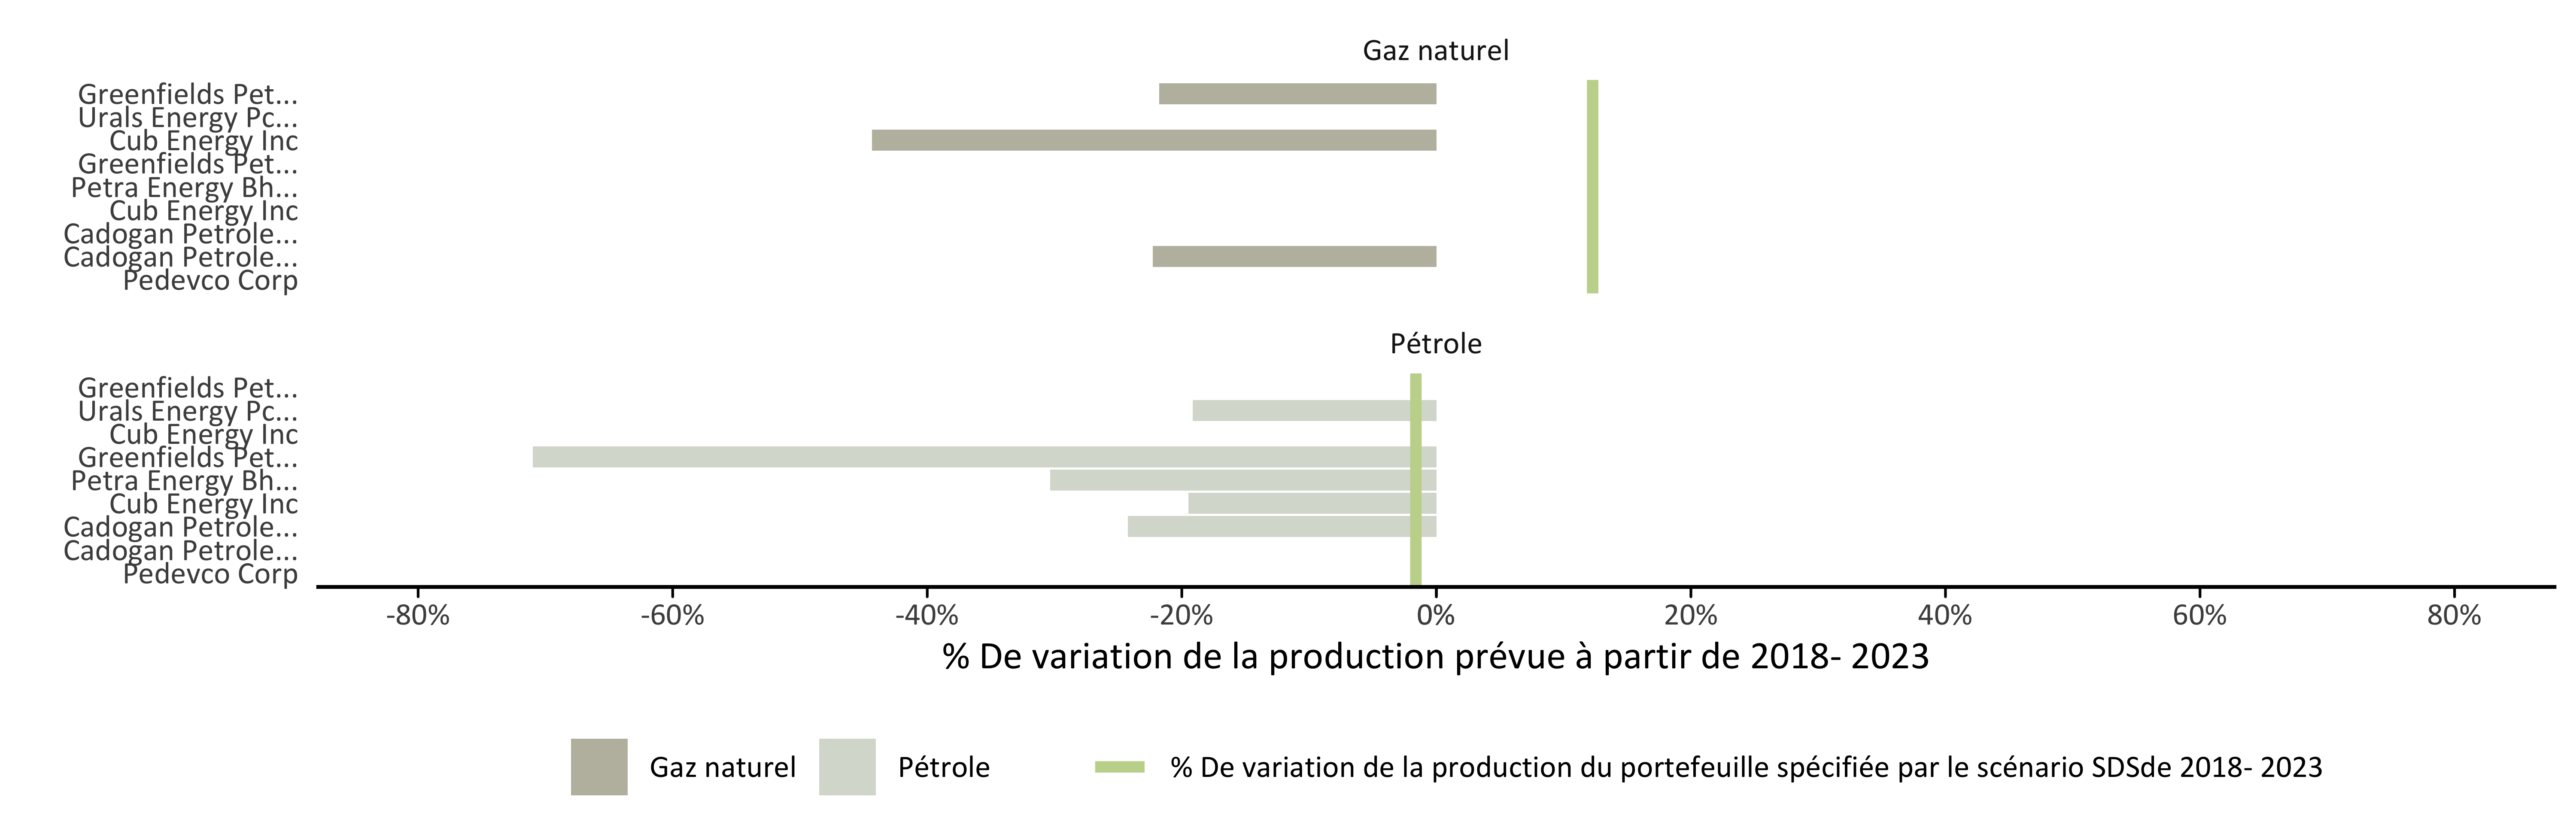
\includegraphics[trim = {0 0cm 0 0},width=1\linewidth]{ReportOutputs/Fig46}
\end{center}
%	\vspace{-.5cm}


	\PageFooter{5 - EXPOSICIÓN DE LAS EMPRESAS}
	

	
	\newpage
	%FossilFuelSector_EQE
	\section*{} % CONTRIBUTIONS OF SECURITIES TO THE RESULTS
	\HeaderDouble{CONTRIBUCIÓN DE LOS TÍTULOS FINANCIEROS A LOS RESULTADOS }{PETRÓLEO Y GAS }

	
	%CarbonBudgetS
	\textbf{Alineación del presupuesto de carbono de las empresas petroleras con mayor participación en la cartera de acciones en Startyear+5.} Esta gráfica se basa en el trabajo de Carbon Tracker Initiative y muestra la alineación del presupuesto de carbono y, por ende, el nivel potencial de exposición a gasto de capital innecesario de los principales productores de petróleo y gas (según el valor de mercado).
	
	\vspace{-.35cm}
	
	\begin{center}
		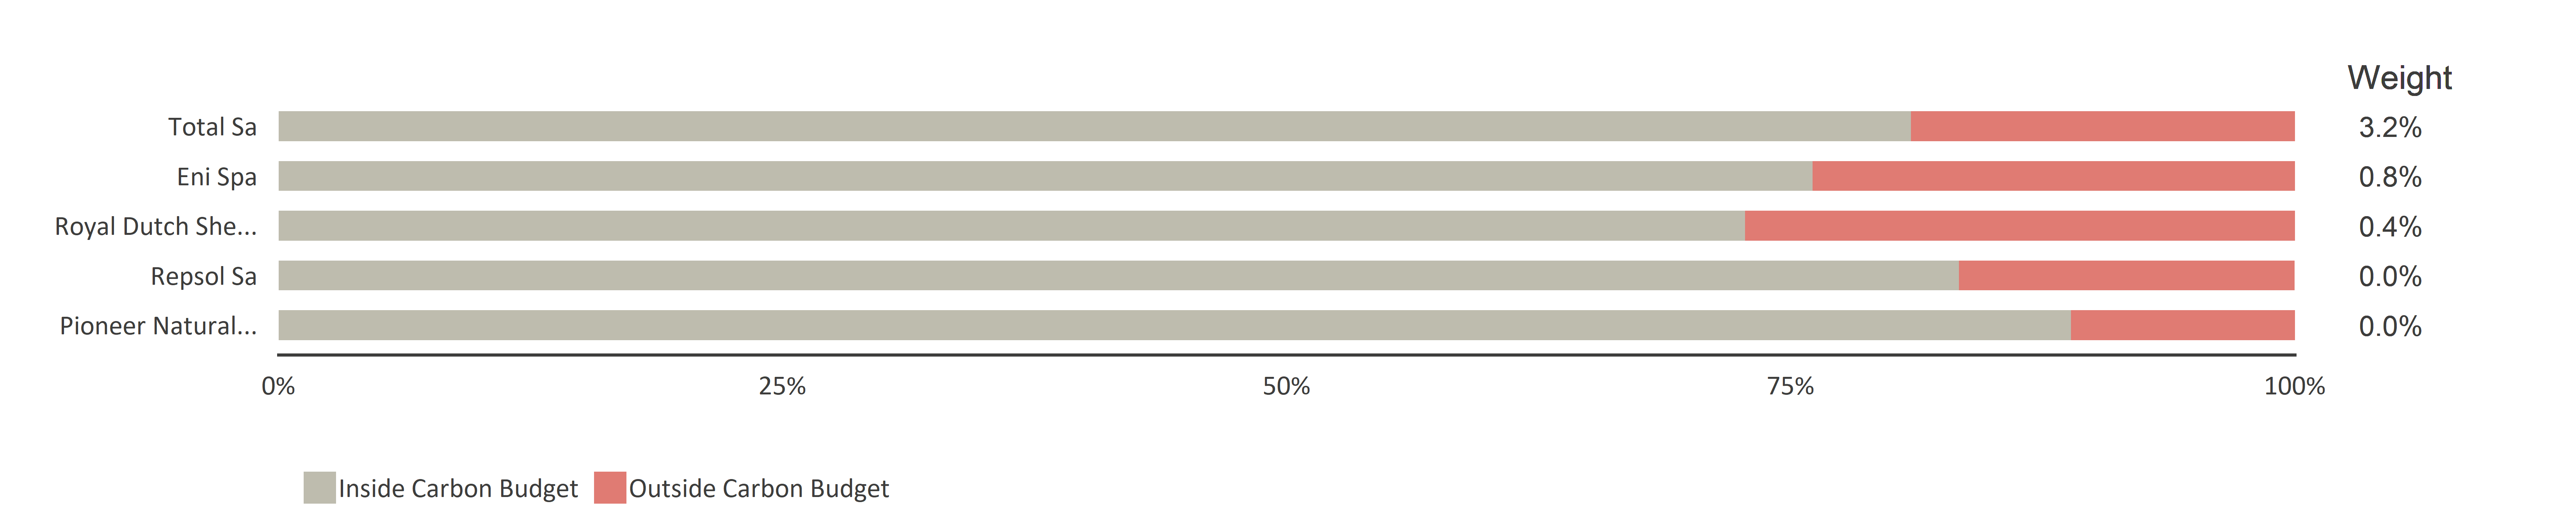
\includegraphics[trim = {0 0cm 0 0},width=1\linewidth]{ReportOutputs/Fig48}
	\end{center}
	%CarbonBudgetE
	%FossilFuelOneSectorS
	\PageFooter{5 -  EXPOSICIÓN DE LAS EMPRESAS}
	
	\newpage
	\section*{} % CONTRIBUTIONS OF SECURITIES TO THE RESULTS
	\HeaderDouble{CONTRIBUCIÓN DE LOS TÍTULOS FINANCIEROS A LOS RESULTADOS }{PETRÓLEO Y GAS }
		%FossilFuelOneSectorE
	
	%FossilFuelSector_CBS
	\textbf{Desglose de la producción petrolera de los principales participantes en la cartera de bonos corporativos en Startyear+5.}
	Esta gráfica muestra la producción de petróleo por tipo de hidrocarburo para las principales empresas (según el valor de mercado) de producción de petróleo en la cartera de bonos corporativos.
	
	\vspace{-.35cm}
	
	\begin{center}
		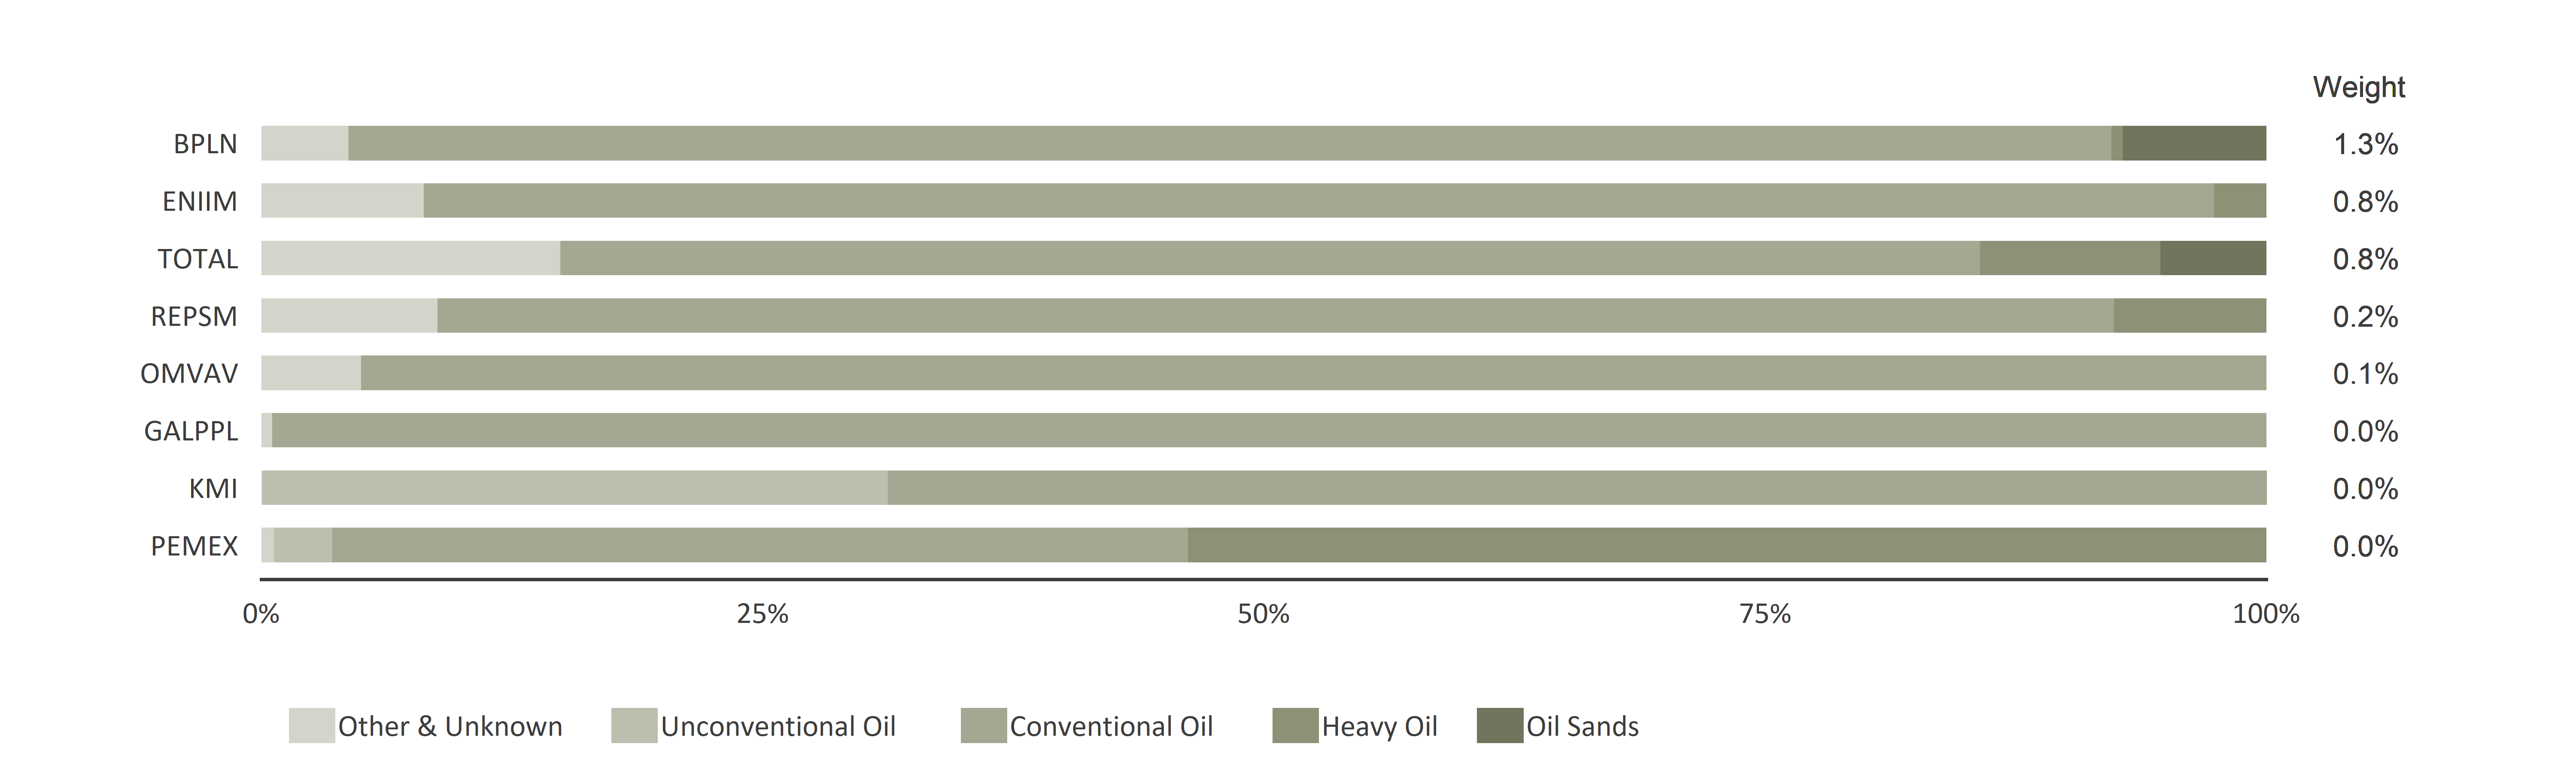
\includegraphics[trim = {0 0cm 0 0},width=1\linewidth]{ReportOutputs/Fig43}
	\end{center}
	%FossilFuelSector_CBE
	
	%FossilFuelSector_EQS
	\textbf{Desglose de la producción petrolera de los principales participantes en la cartera de acciones en Startyear+5.}
	Esta gráfica muestra la producción de petróleo por tipo de hidrocarburo para las principales empresas (según el valor de mercado) de producción de petróleo en la cartera de acciones.
	
	
	
	\vspace{-.35cm}
	
	\begin{center}
		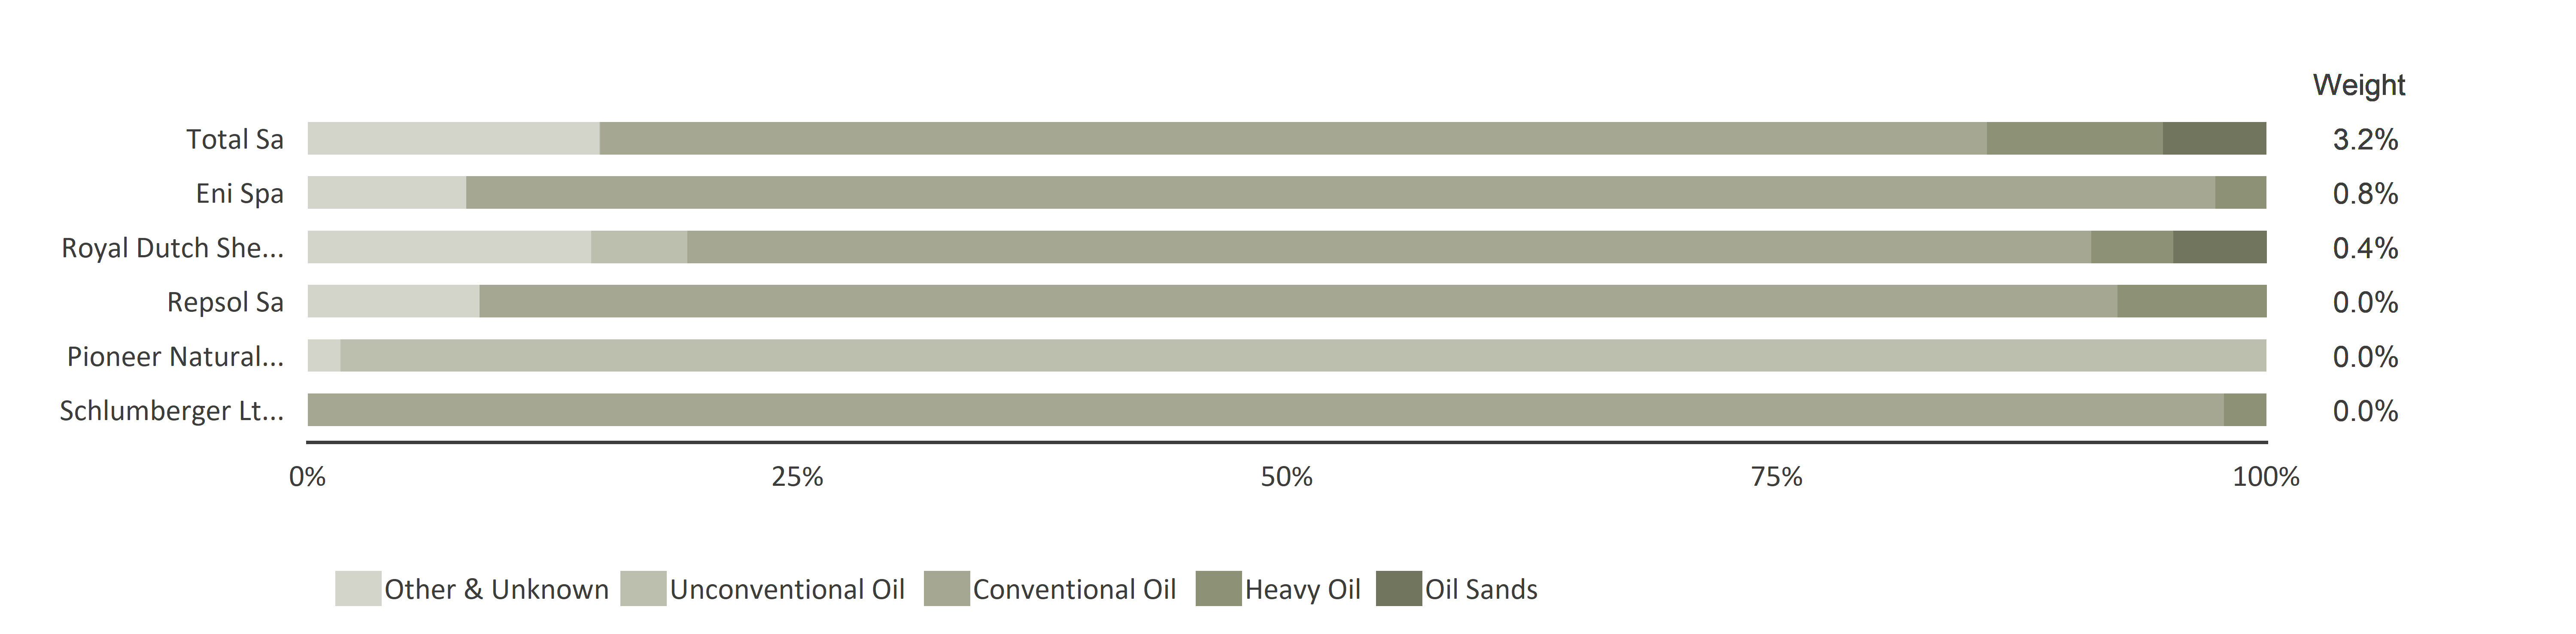
\includegraphics[trim = {0 0cm 0 0},width=1\linewidth]{ReportOutputs/Fig47}
	\end{center}


	%FossilFuelSector_EQE 
	\PageFooter{5 -  EXPOSICIÓN DE LAS EMPRESAS}
	
	\newpage

	
	%FossilFuelSector_ALLE
	
	
 	%PowerSector_ALLS
	\section*{} % CONTRIBUTIONS OF SECURITIES TO THE RESULTS
	%PowerAutoOneSectorS
	\HeaderDouble{CONTRIBUCIÓN DE LOS TÍTULOS FINANCIEROS A LOS RESULTADOS}{SECTOR ELÉCTRICO}
	%PowerAutoOneSectorE
	

	
		\textbf{Las siguientes gráficas muestran la combinación actual esperada de tecnologías de generación de energía en Startyear+5 de las principales empresas de electricidad (según el valor de mercado) en las carteras de bonos y acciones.} 
		
		
		
		Los resultados mostrados son comparados con la combinación actual de energía planeada de la cartera, la combinación de energía objetivo bajo el ScenarioValue, y la combinación de energía planeada en un mercado alineado en Startyear+5. La ponderación dada muestra el peso de la inversión total en cada empresa expresada como porcentaje del valor total de la cartera. 
		
		
		
	
	%PowerSector_CBS
	\textbf{Desglose por tecnología para empresas del sector eléctrico en la cartera de bonos corporativos}
	\vspace{-.0cm}
	
	\begin{center}
		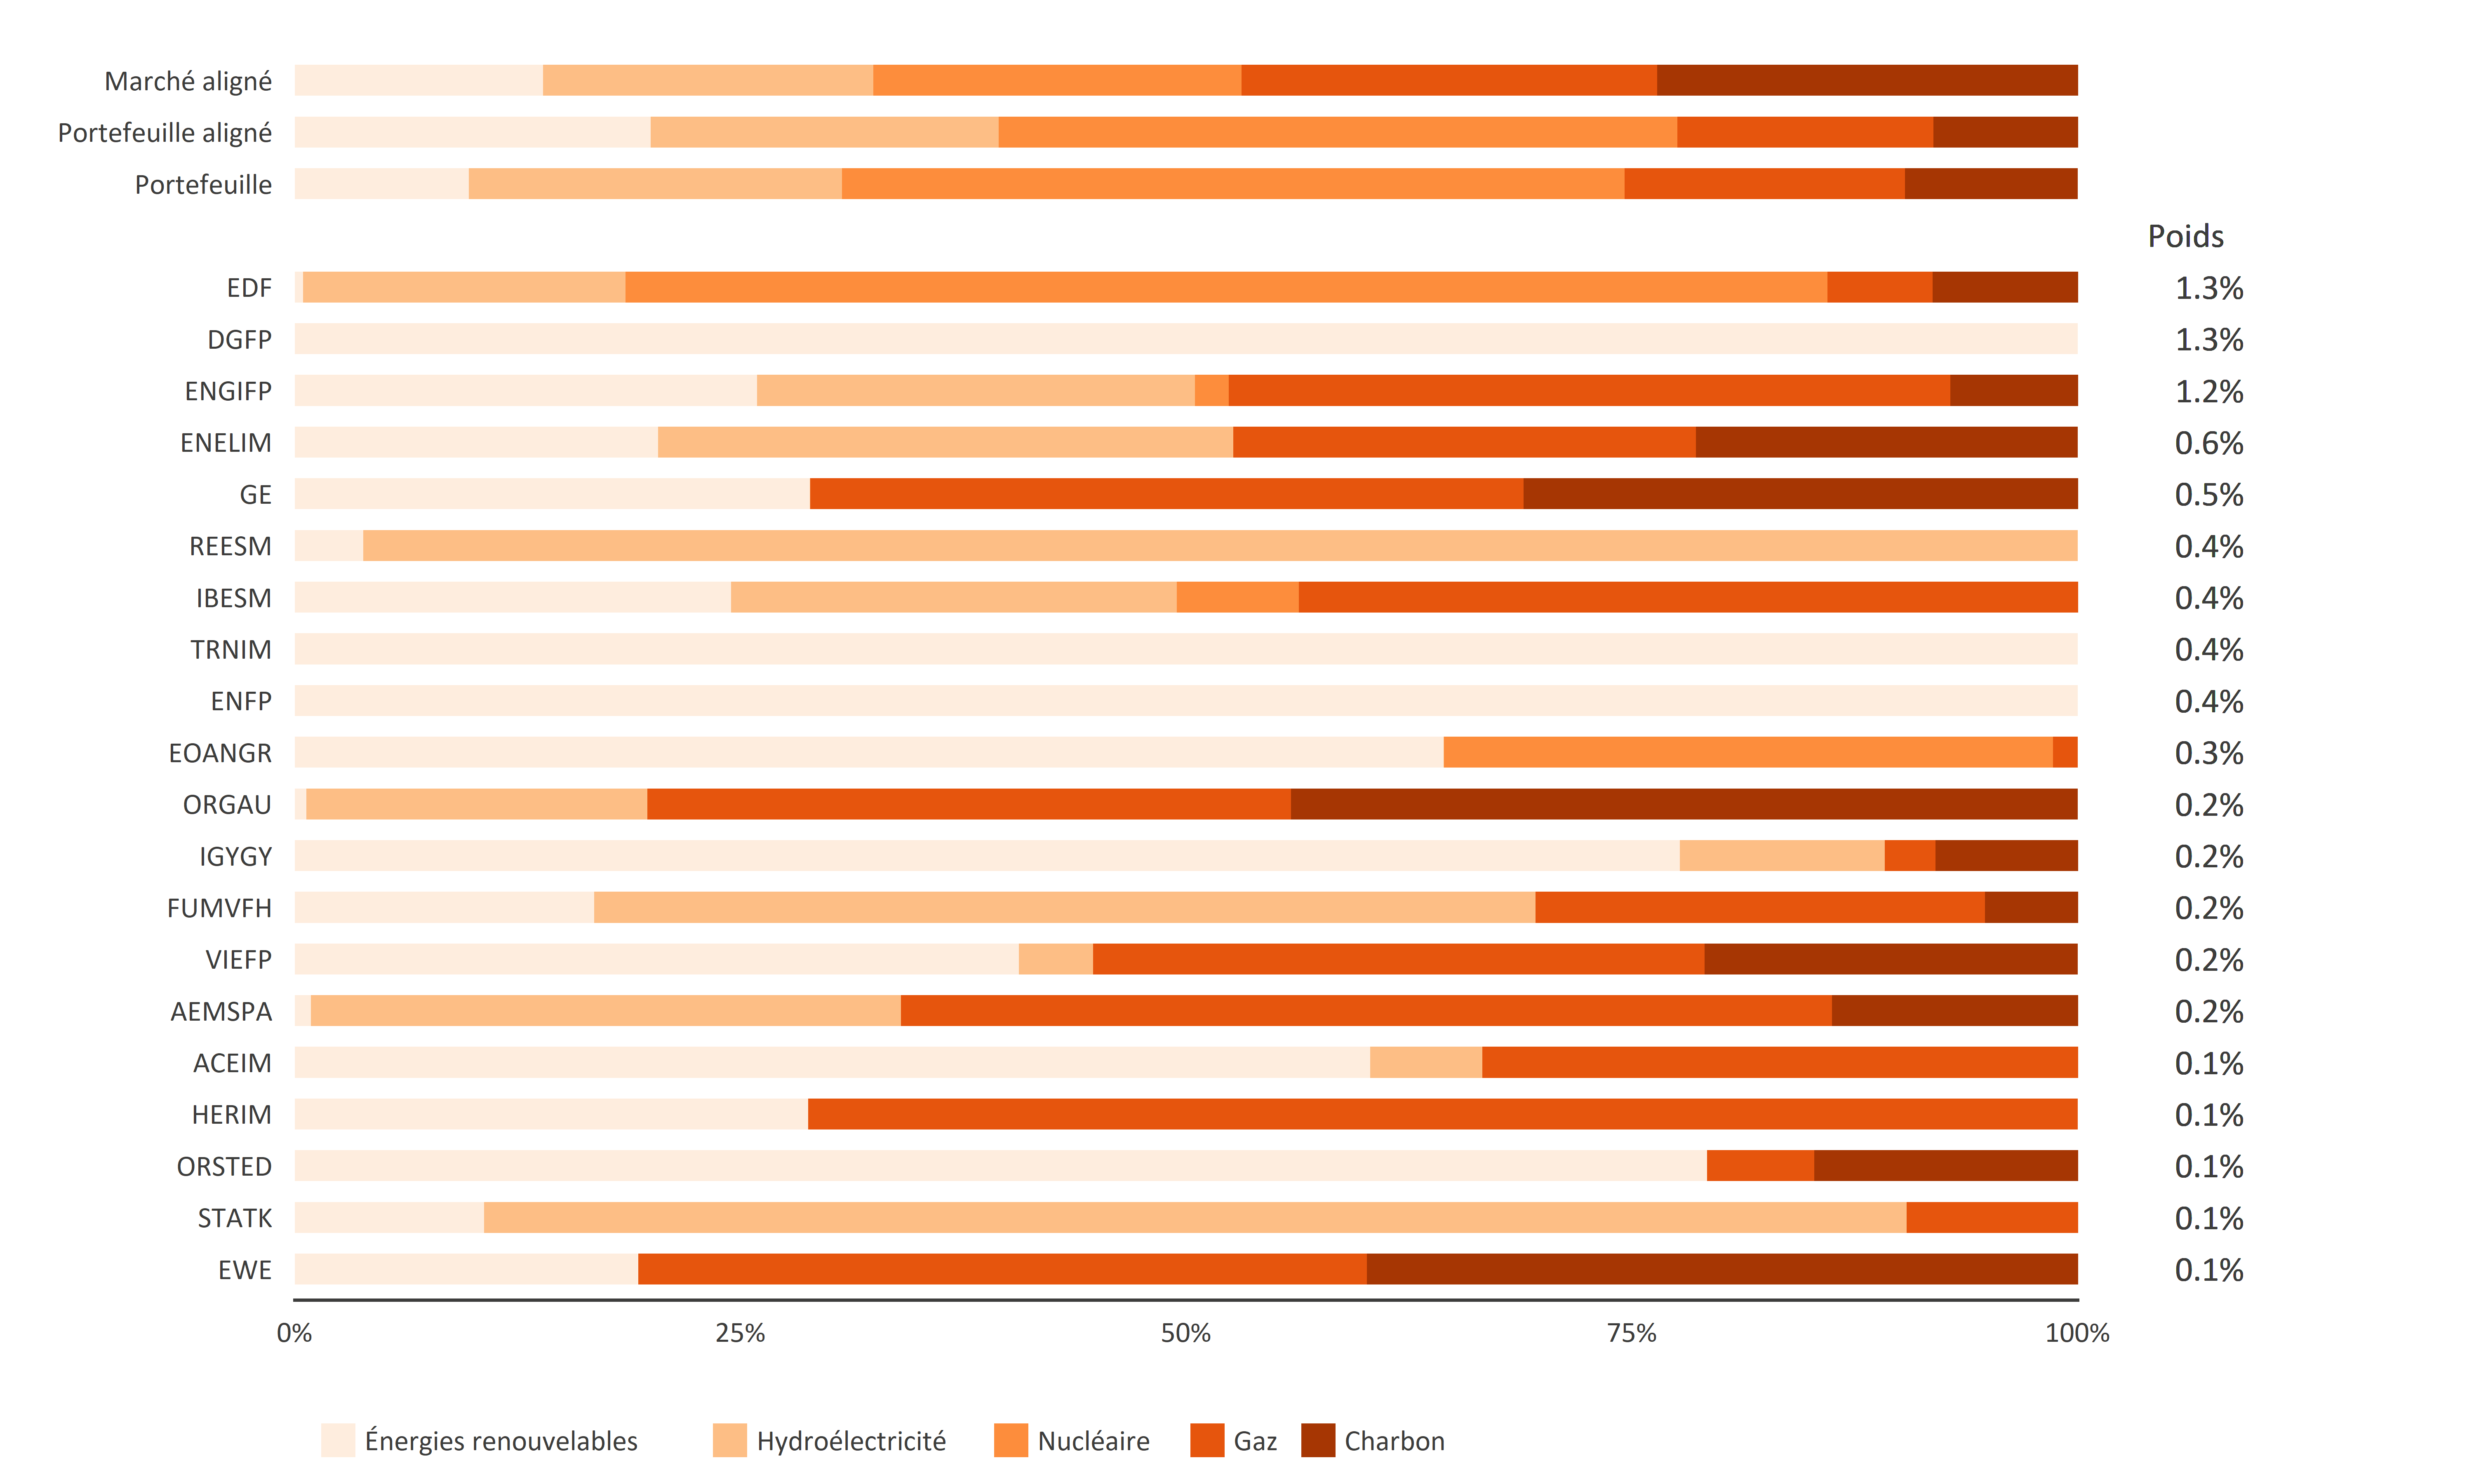
\includegraphics[trim = {0 0cm 0 0},width=1\linewidth]{ReportOutputs/Fig40}
	\end{center}
	%PowerSector_CBE
	%PowerSector_EQS
	\textbf{Desglose por tecnología para empresas del sector eléctrico en la cartera de acciones}
	\vspace{-.0cm}
	
	\begin{center}
		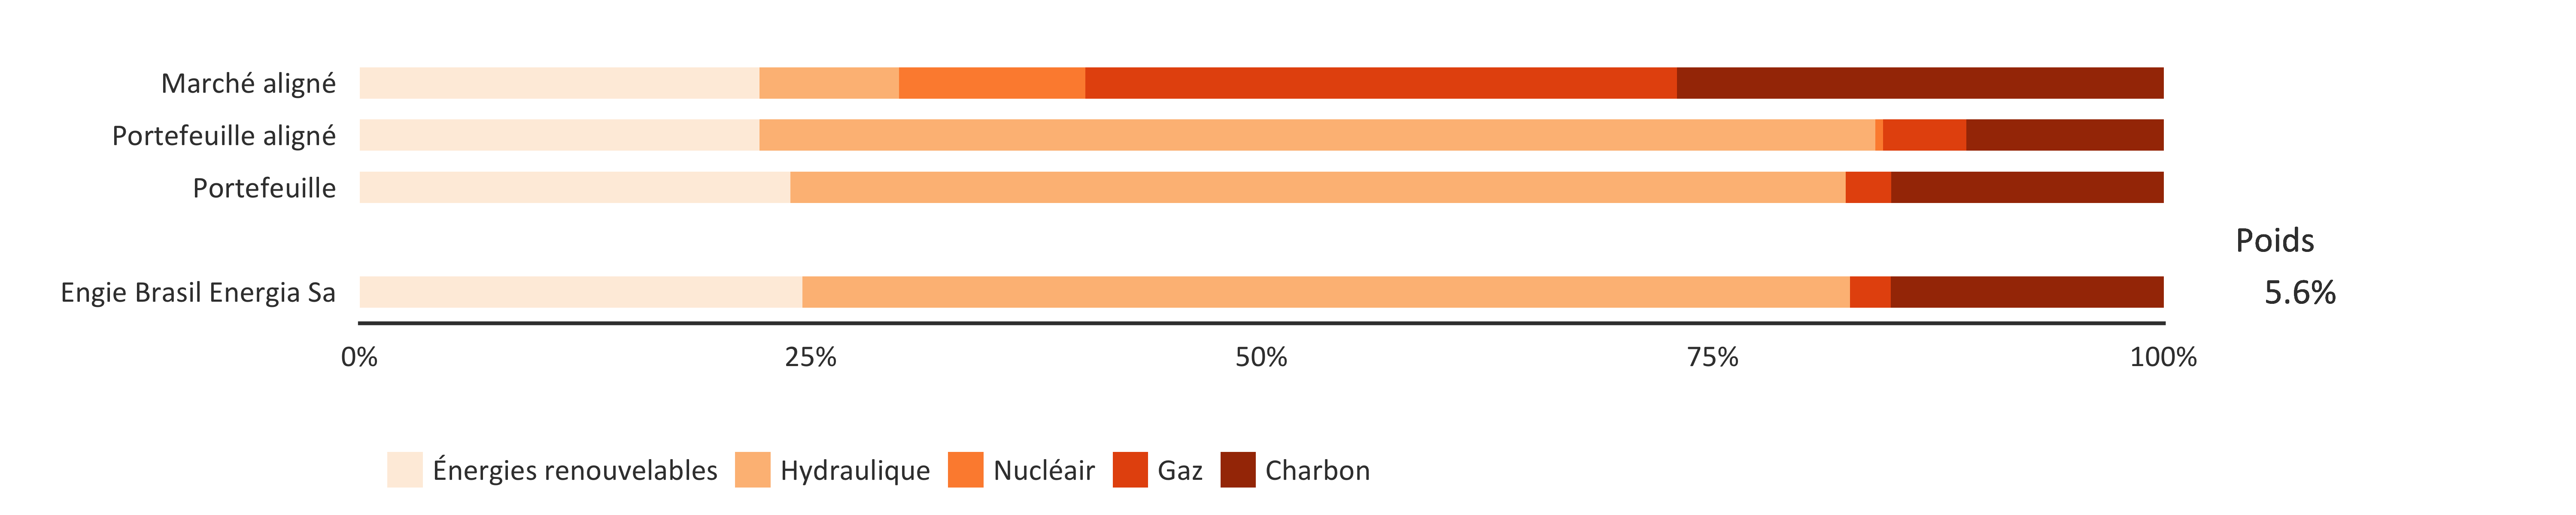
\includegraphics[trim = {0 0cm 0 0},width=1\linewidth]{ReportOutputs/Fig44}
	\end{center}		
	%PowerSector_EQE
	
	%PowerAutoOneSectorS
	%\PageFooterFifth
	\PageFooter{5 - EXPOSICIÓN DE LAS EMPRESAS}
	
	\newpage
	%PowerSector_ALLE
	%AutoSector_ALLS
	\section*{} % CONTRIBUTIONS OF SECURITIES TO THE RESULTS 
	\HeaderDouble{CONTRIBUCIÓN DE LOS TÍTULOS FINANCIEROS A LOS RESULTADOS}{SECTOR AUTOMOTRIZ}
	%PowerAutoOneSectorE
	
		\textbf{Los siguientes gráficos muestran la combinación esperada actual de tecnologías de motorización de vehículos en Startyear+5 para los principales fabricantes de automóviles (según el valor de mercado) en las carteras de bonos y acciones.} 
		
		
		Los resultados mostrados son comparados con la combinación actual de producción planeada de la cartera, la combinación de producción objetivo bajo el ScenarioValue, y la combinación de producción planeada en el mercado alineado en Startyear+5. La ponderación dada muestra el tamaño de la inversión total en cada empresa expresada como porcentaje del valor total de la cartera.
		
	
	%AutoSector_CBS
	\textbf{Desglose por tecnología de empresas automotrices en la cartera de bonos corporativos}
	\vspace{-.0cm}
	
	\begin{center}
		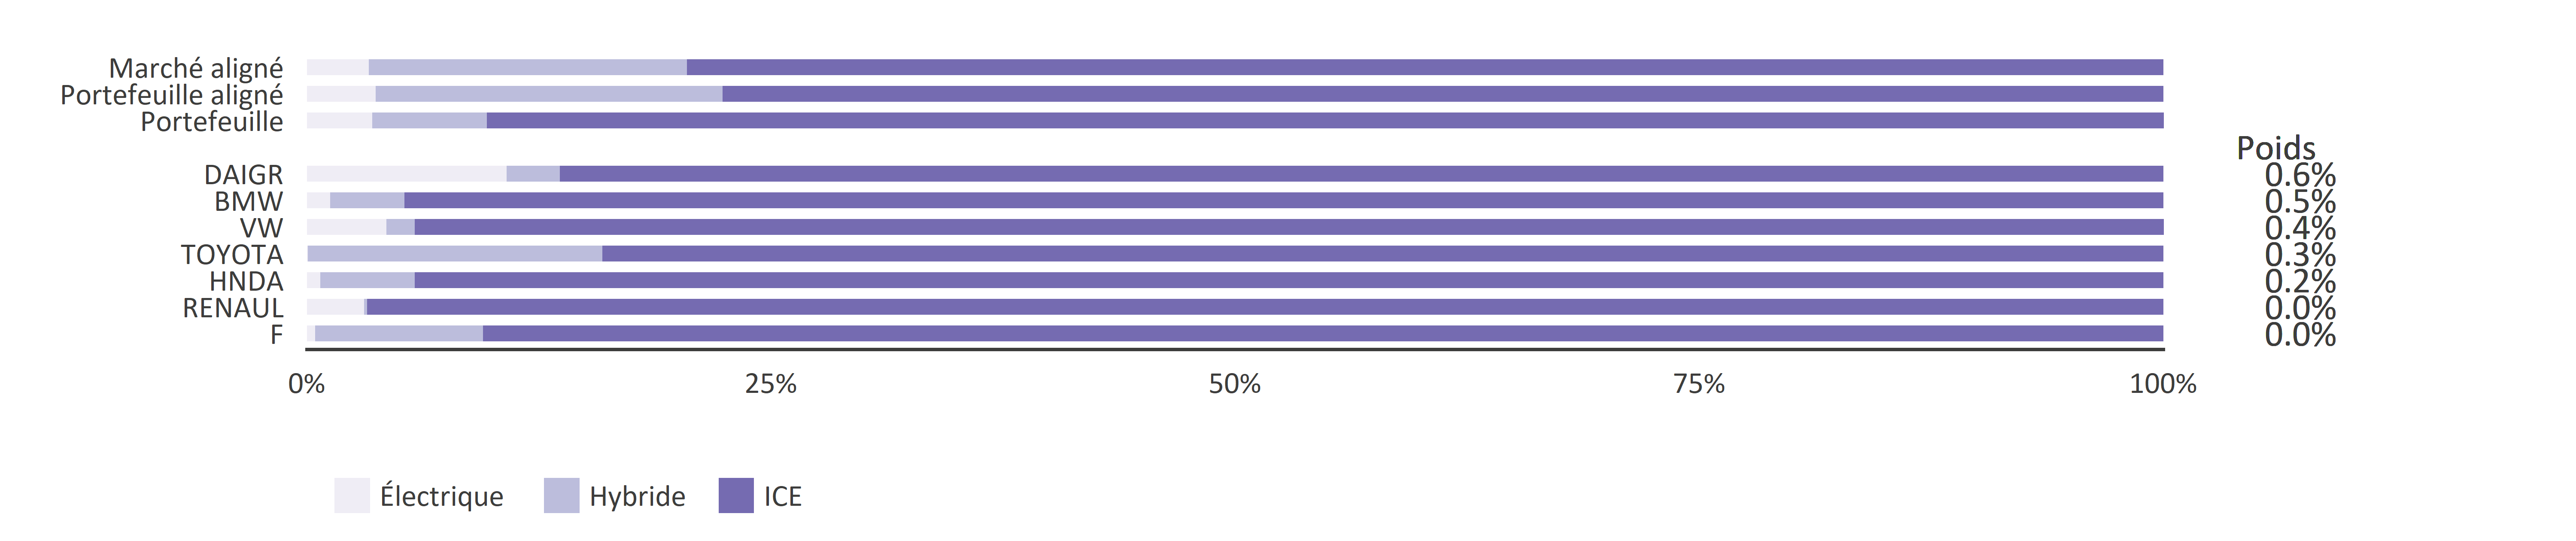
\includegraphics[trim = {0 0cm 0 0},width=1\linewidth]{ReportOutputs/Fig41}
	\end{center}
	%AutoSector_CBE
	
	%AutoSector_EQS
	\textbf{Desglose por tecnología de empresas automotrices en la cartera de acciones}
	\vspace{-.0cm}
	
	\begin{center}
		
\includegraphics[trim = {0 0cm 0 0},width=1\linewidth]{ReportOutputs/Fig45}
	\end{center}
	%AutoSector_EQE
	
	%\PageFooterFifth
\PageFooter{5 - EXPOSICIÓN DE LAS EMPRESAS}
	
	\newpage 
	%AutoSector_ALLE 
	
	%PowerSector_ALLS
	%CoalCapChartS
	\section*{} % COAL RETIREMENTS 
	\HeaderDouble{PROPIEDAD ACTIVA}{ELECTRICIDAD A CARBÓN}
	
Las siguientes graficas muestran los retiros requeridos y adiciones de capacidad excesivas de las empresas presentes en la cartera en Startyear+10 para alinearse con el ScenarioValue. Como la capacidad debería disminuir bajo el ScenarioValue, toda la capacidad instalada nueva debe compensarse con el retiro de la capacidad existente; esto se representa como una adición de capacidad.  Los retiros requeridos representan la capacidad existente que debe ser retirada además de la capacidad adicional.   
	
	%CBSpecificS
	\textbf{Retiros requeridos y adiciones de capacidad de carbón de empresas en la cartera de bonos corporativos.}
	\vspace{-.0cm}
	
	\begin{center}
		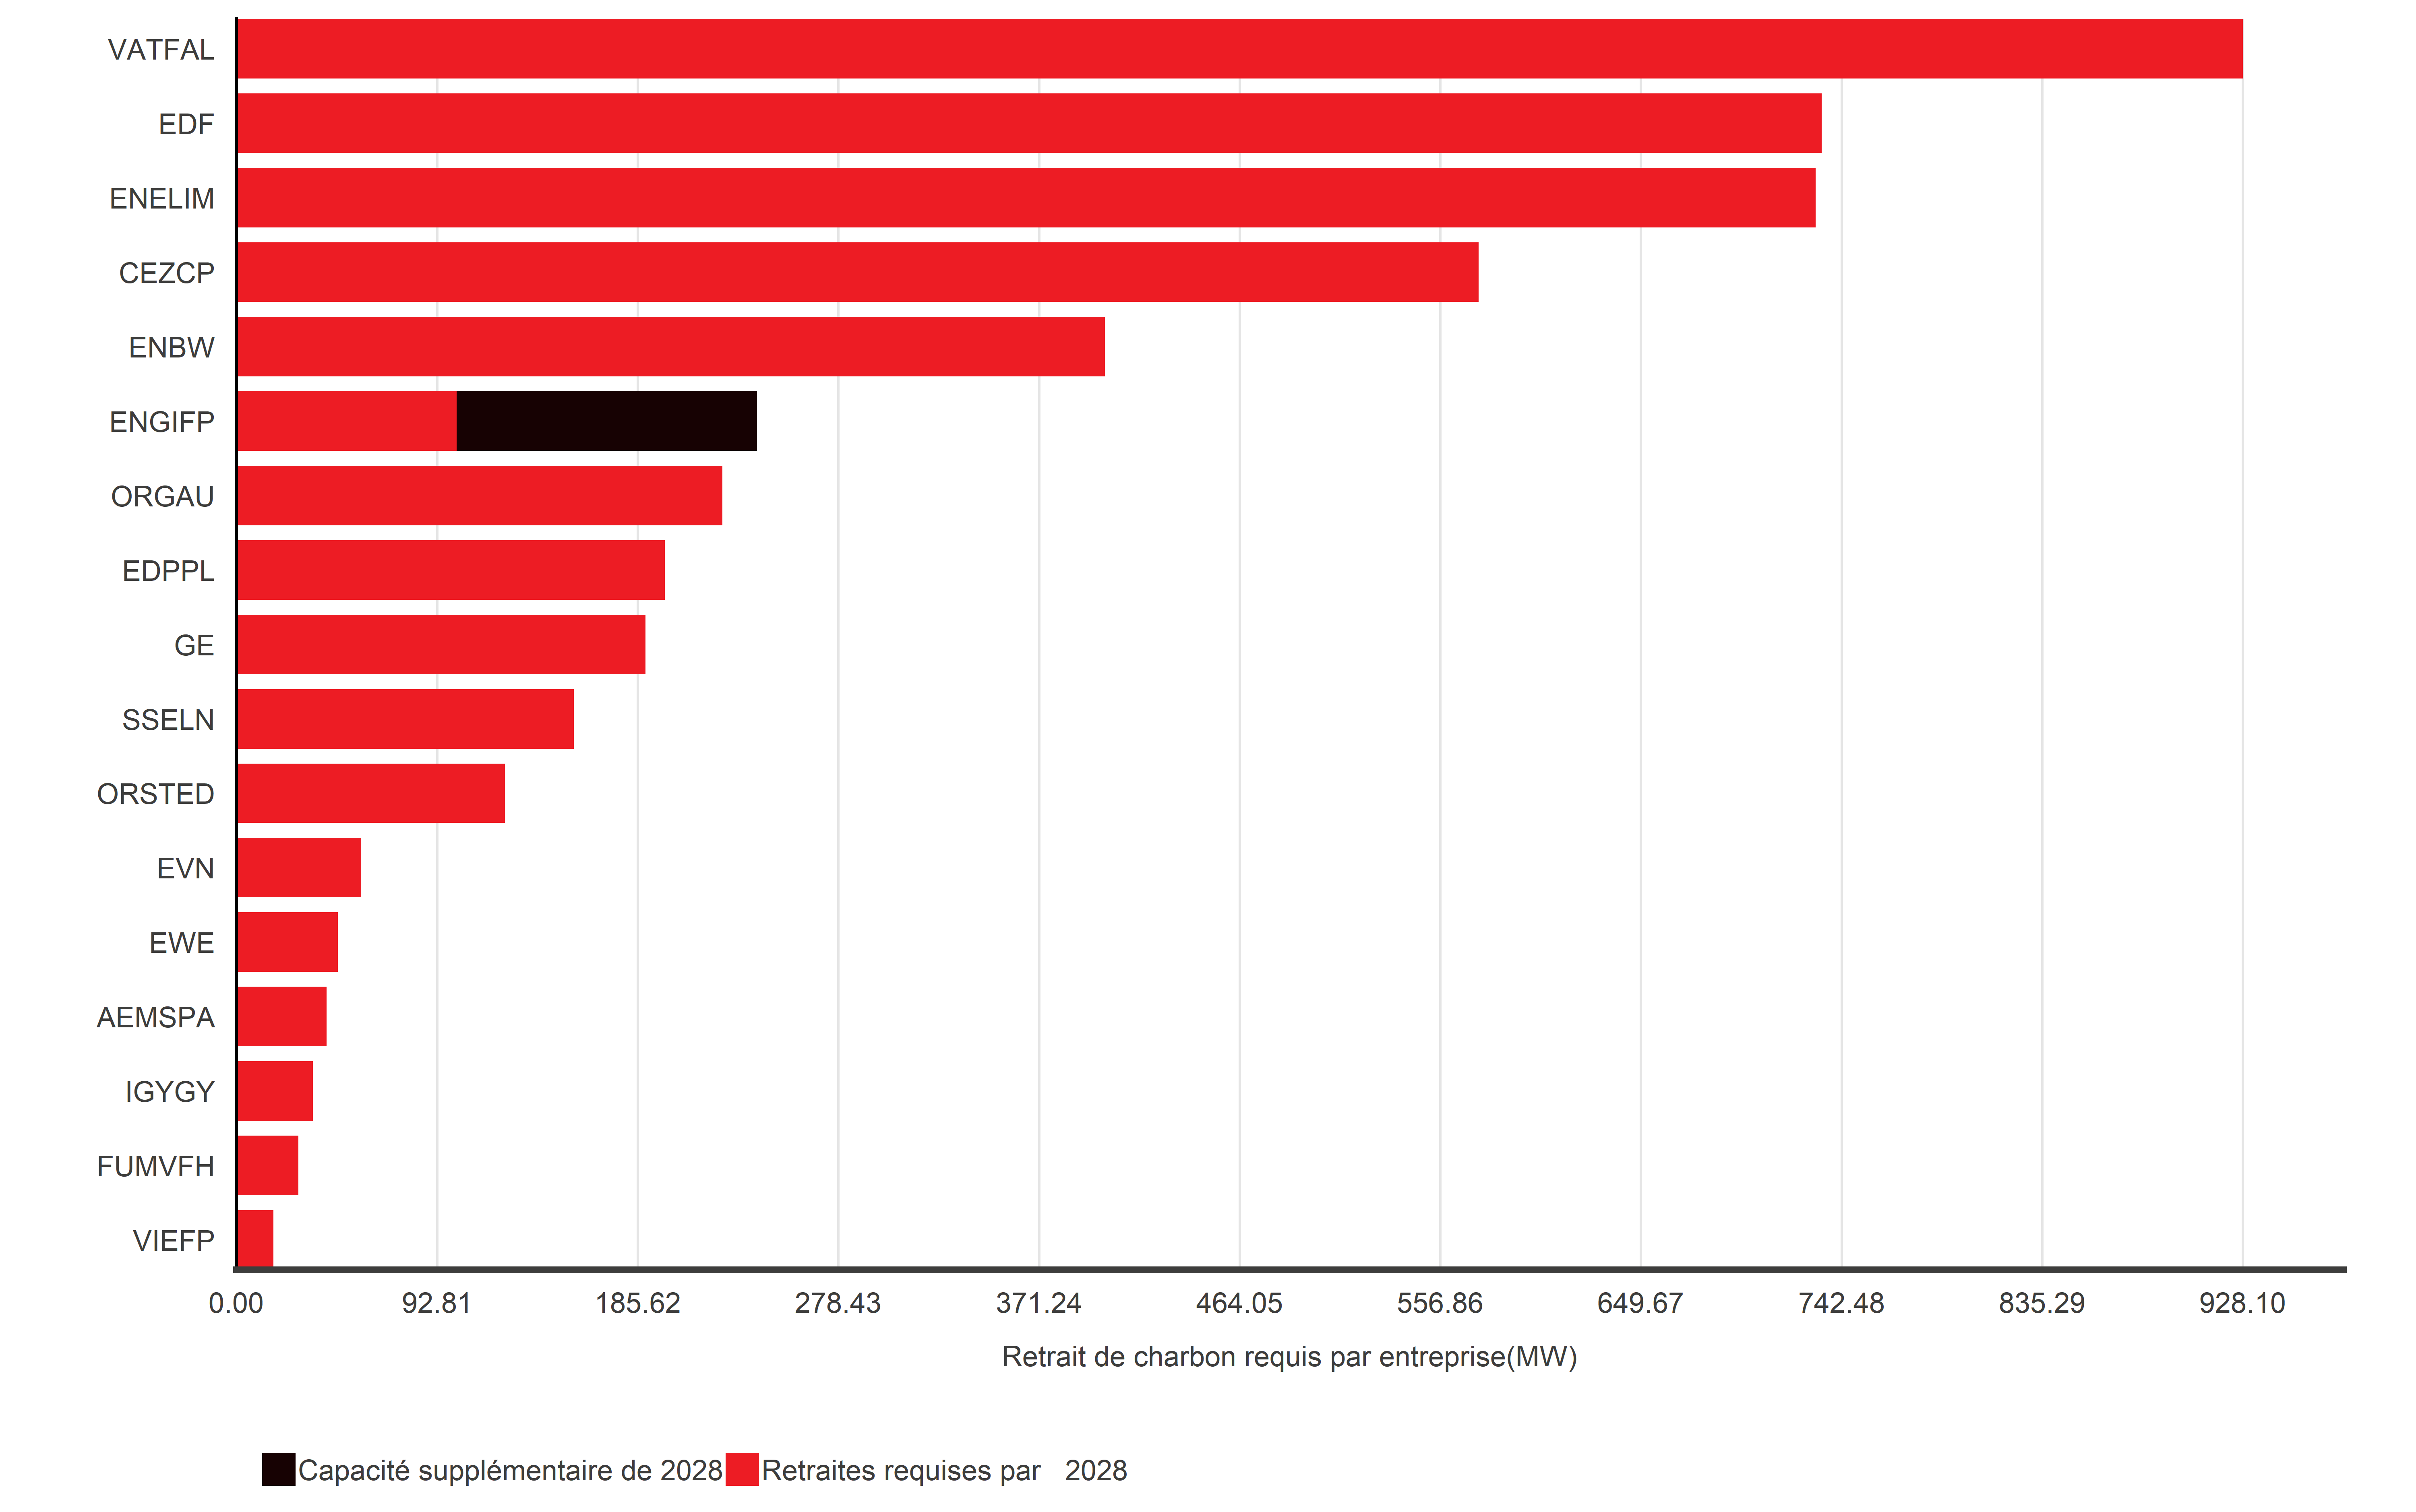
\includegraphics[trim = {0 0cm 0 0},width=1\linewidth]{ReportOutputs/Fig62}
	\end{center}
	%CBSpecificE
	
	%EQSpecificS	
	\textbf{Retiros requeridos y adiciones de capacidad de carbón de empresas en la cartera de acciones}
	\vspace{-.0cm}
	
	\begin{center}
		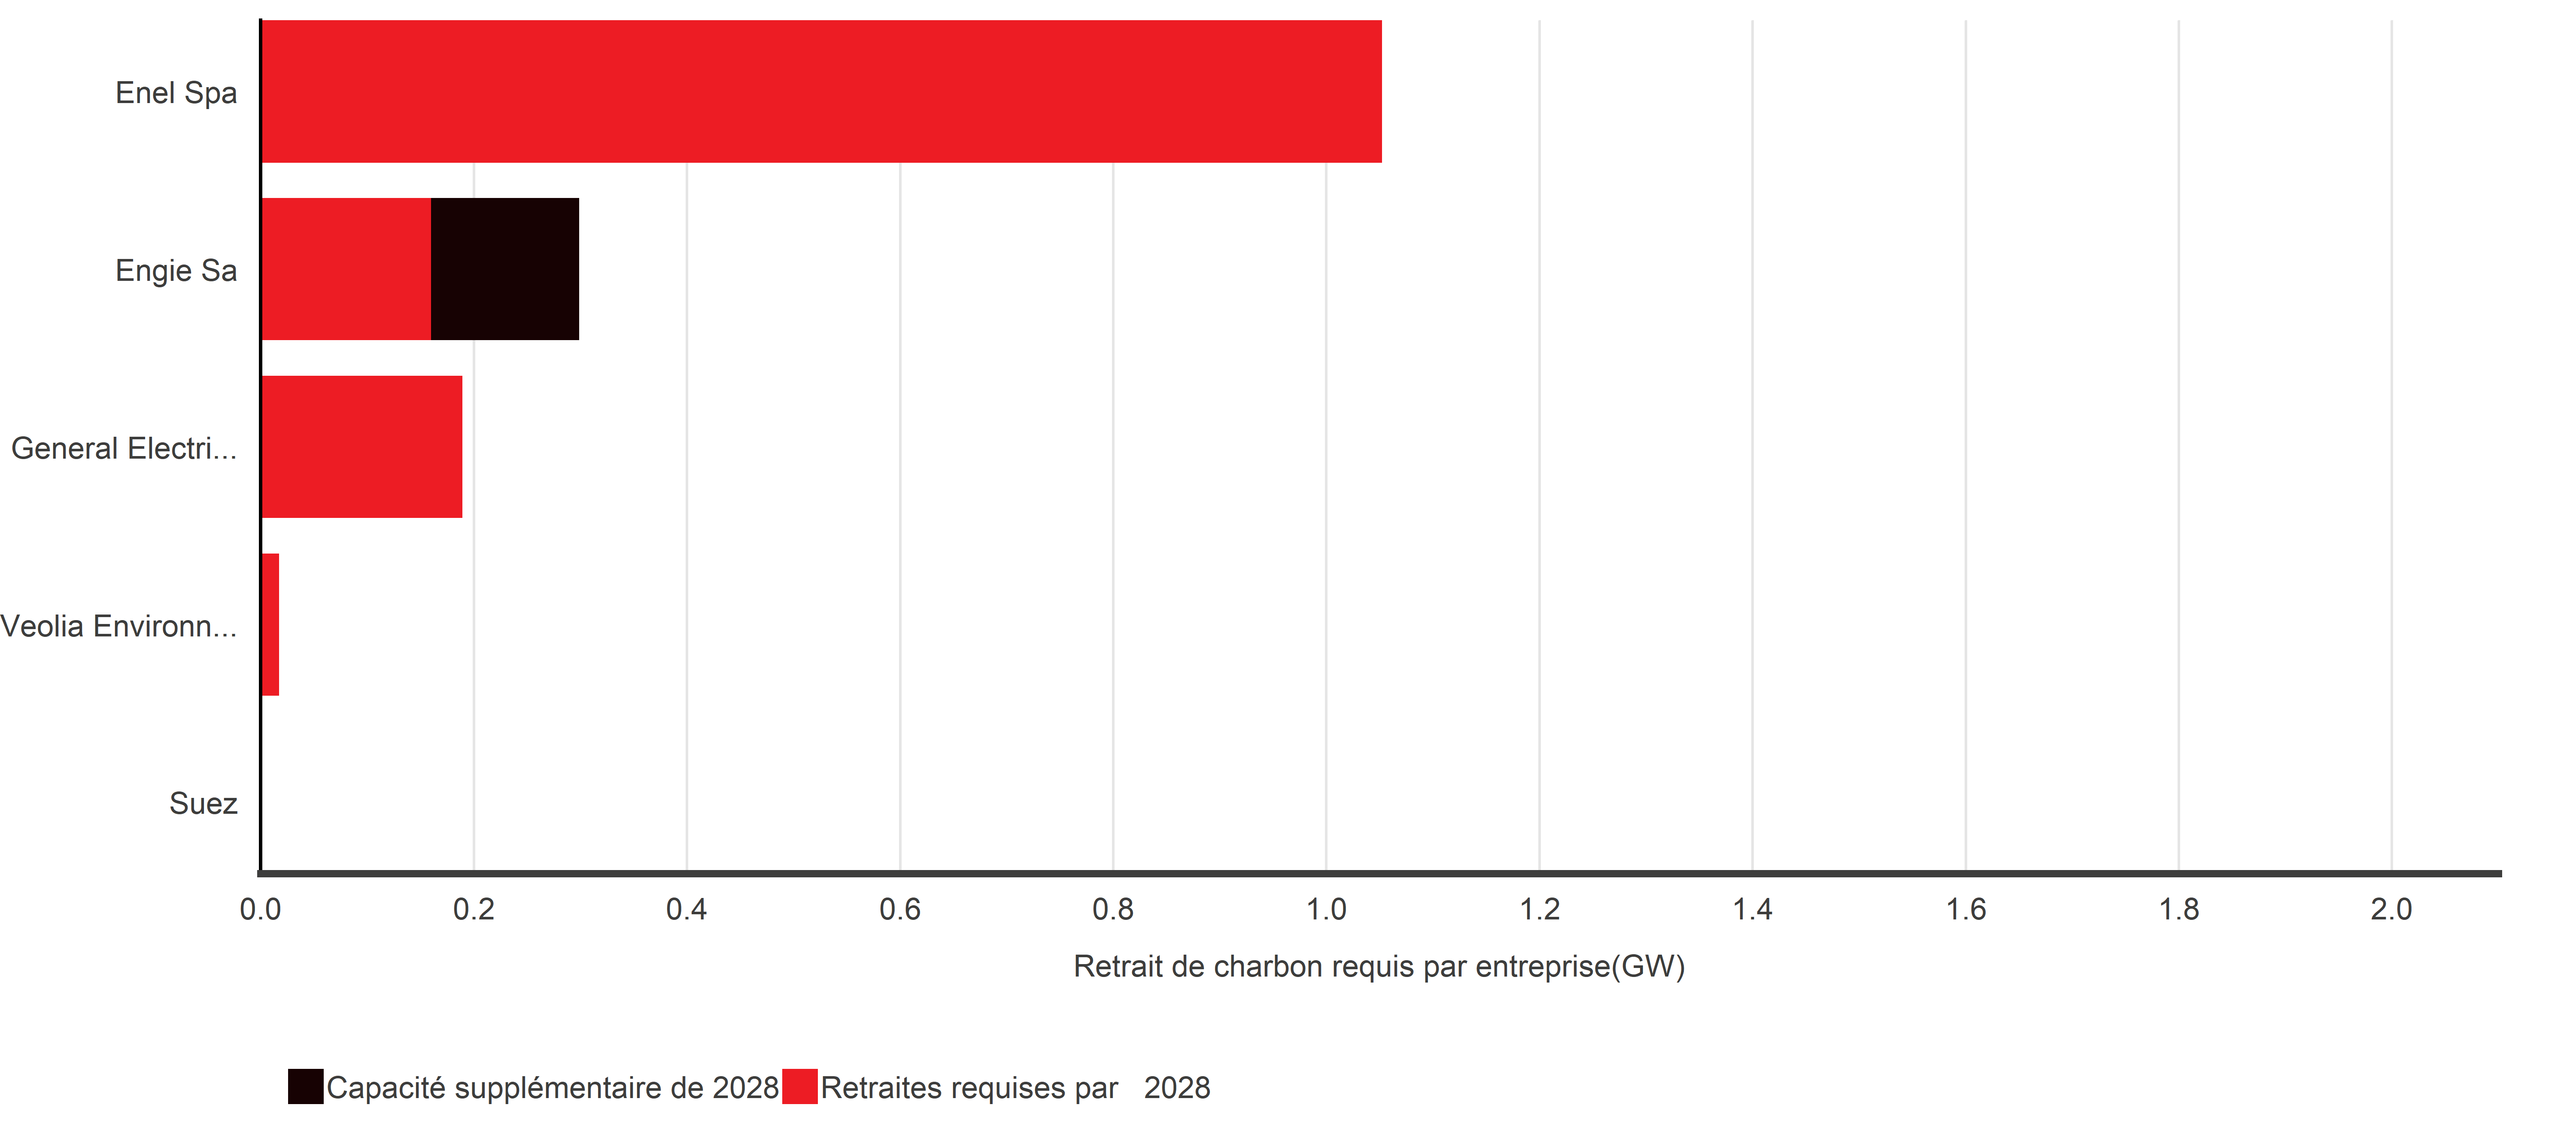
\includegraphics[trim = {0 0cm 0 0},width=1\linewidth]{ReportOutputs/Fig63}
	\end{center}
	%EQSpecificE

	%\PageFooterFifth
\PageFooter{5 - EXPOSICIÓN DE LAS EMPRESAS}
	
	\newpage 
	%CoalCapChartE
	%RenewableCapChartS
	\section*{} % COAL RETIREMENTS 
	\HeaderDouble{PROPIEDAD ACTIVA}{RENOVABLES}
	
Las siguientes gráficas muestran el aumento necesario en la capacidad de generación de energías renovables en las empresas presentes en la cartera para cumplir con los requerimientos de capacidad definidos en el ScenarioValue para Startyear+5. La barra de color rojo muestra las adiciones de capacidad requeridas para cumplir con la capacidad necesaria definida en el ScenarioValue. La barra de color azul muestra el aumento de capacidad previsto de energías renovables de las empresas en la cartera en los próximos 5 años. La diferencia respecto a la capacidad actual se muestra en las barras.

	
	%CBSpecificS
	\textbf{Adición de capacidad de renovables en las empresas de la cartera de bonos corporativos.}
	\vspace{-.0cm}
	
	\begin{center}
		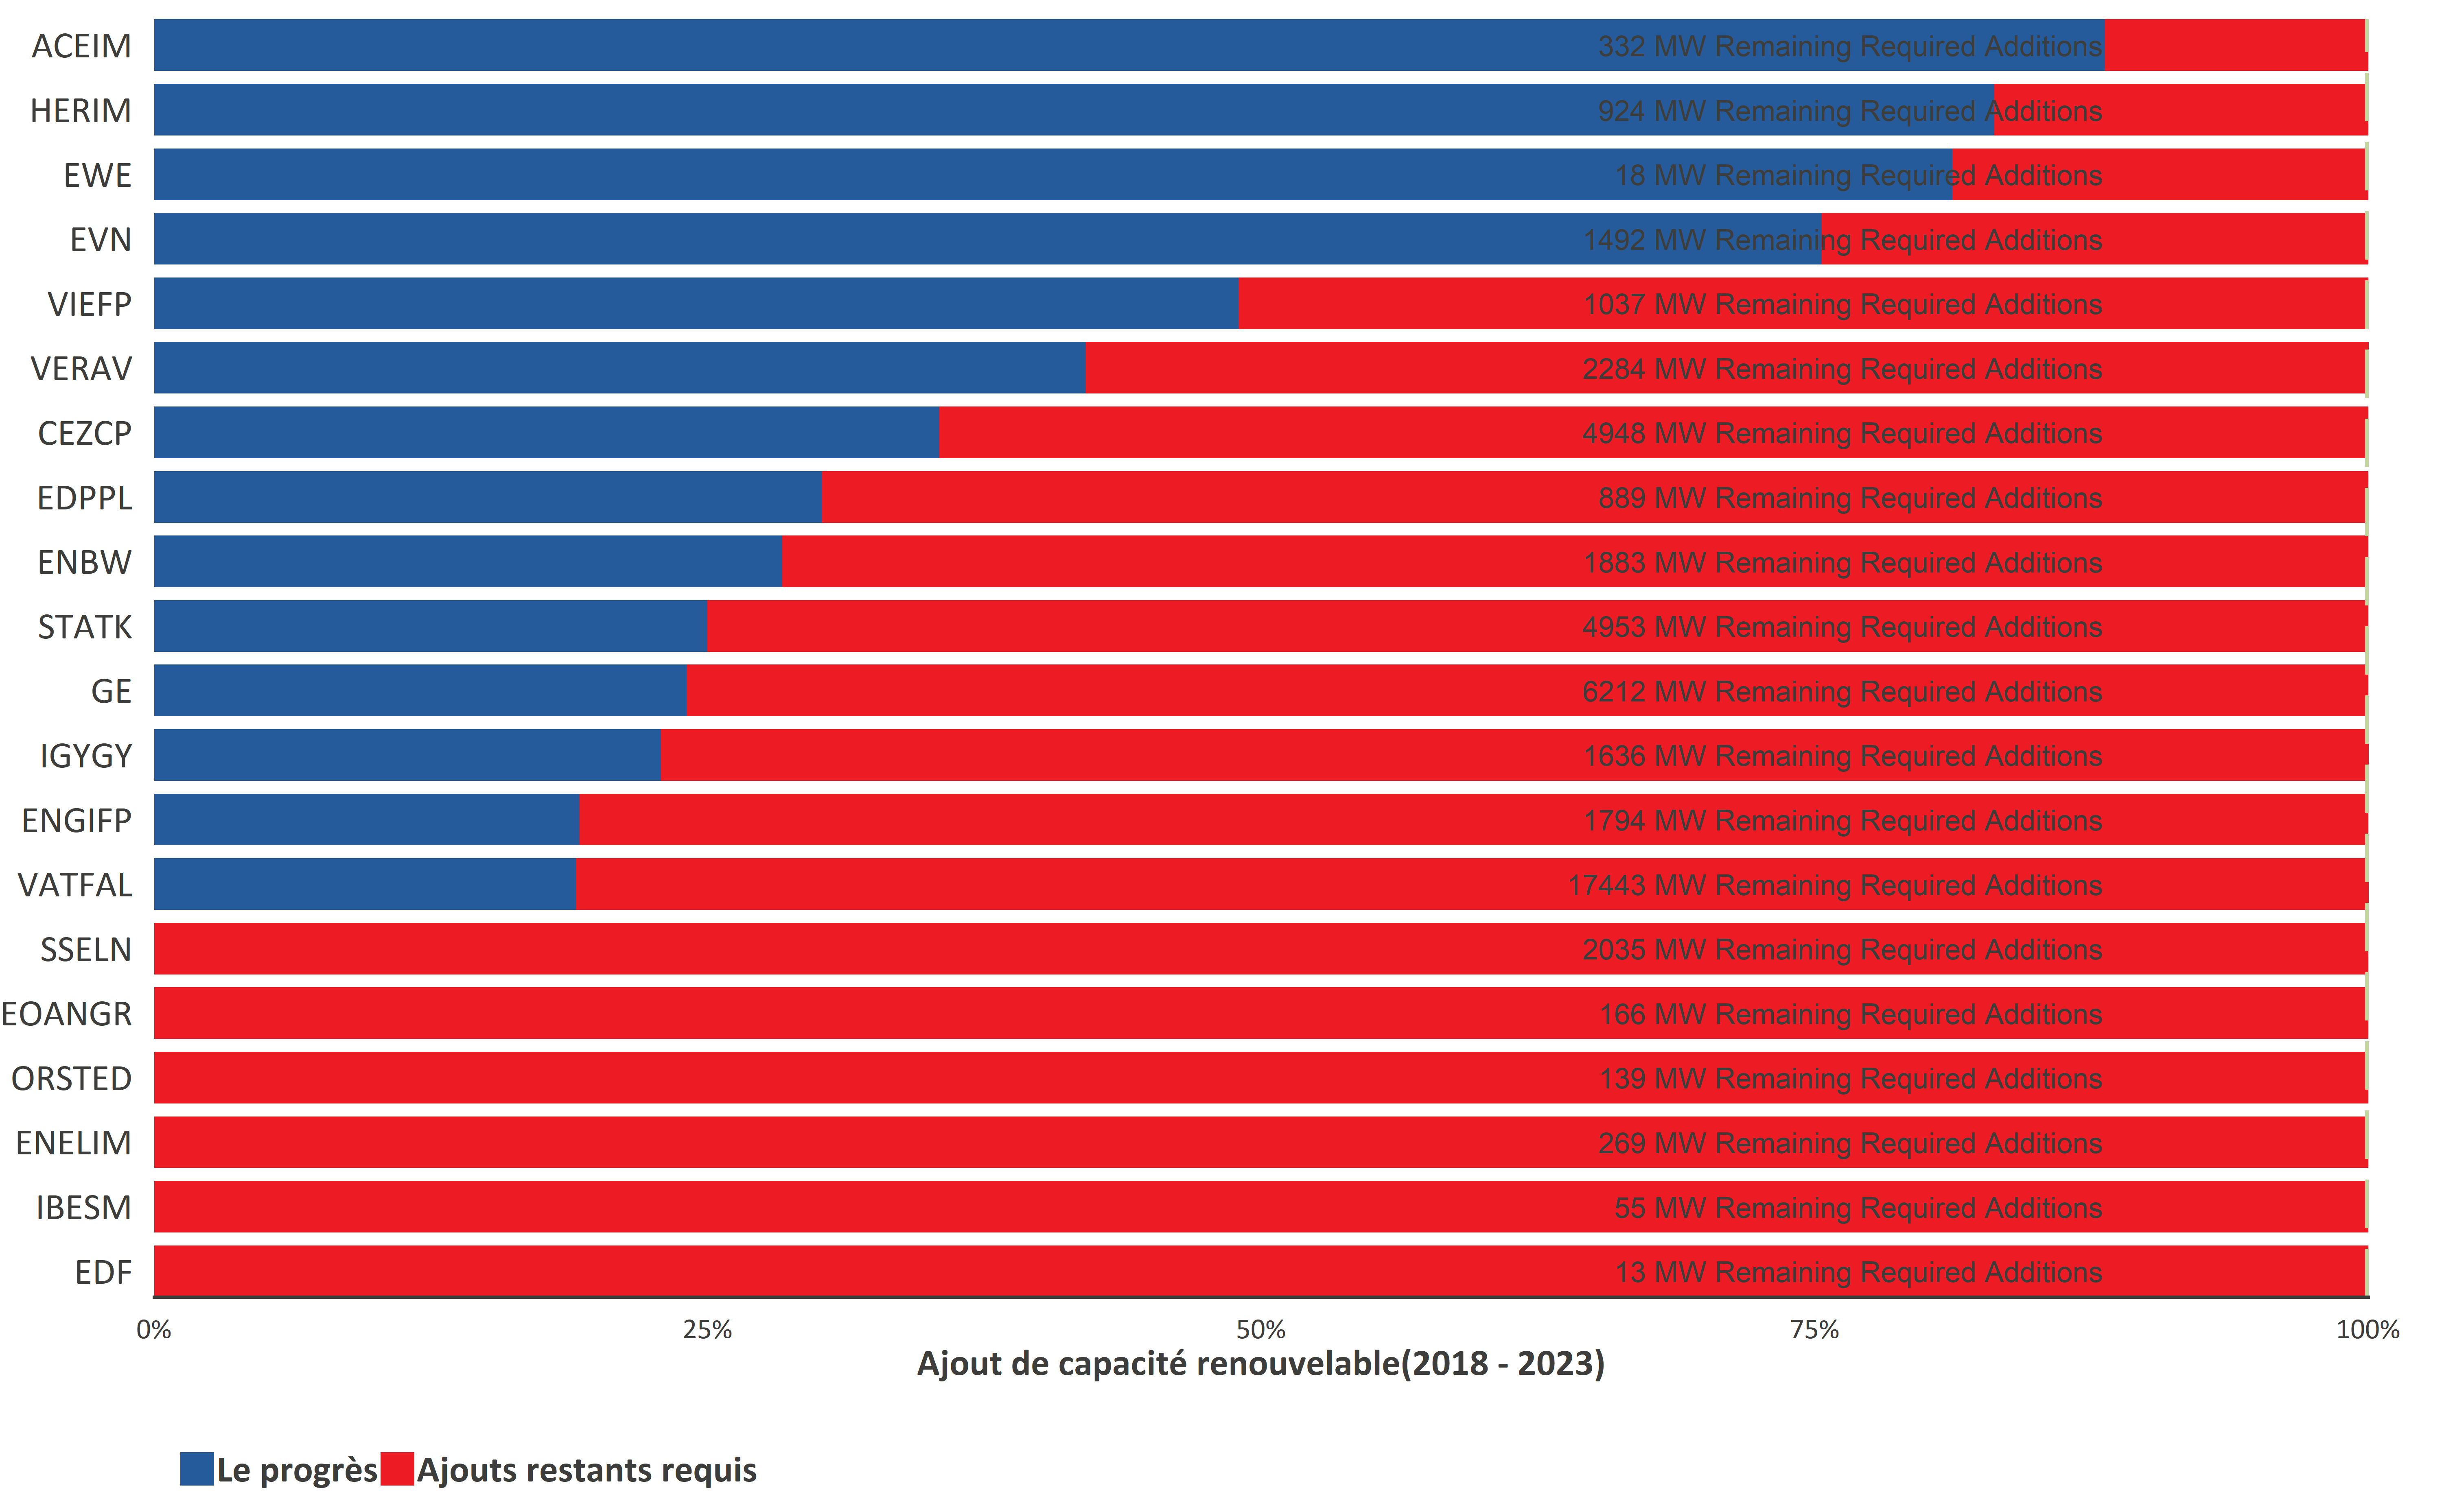
\includegraphics[trim = {0 0cm 0 0},width=1\linewidth]{ReportOutputs/Fig64}
	\end{center}
	%CBSpecificE
	
	%EQSpecificS	
	\textbf{Adición de capacidad de renovables en las empresas en la cartera de acciones.}
	\vspace{-.0cm}
	
	\begin{center}
		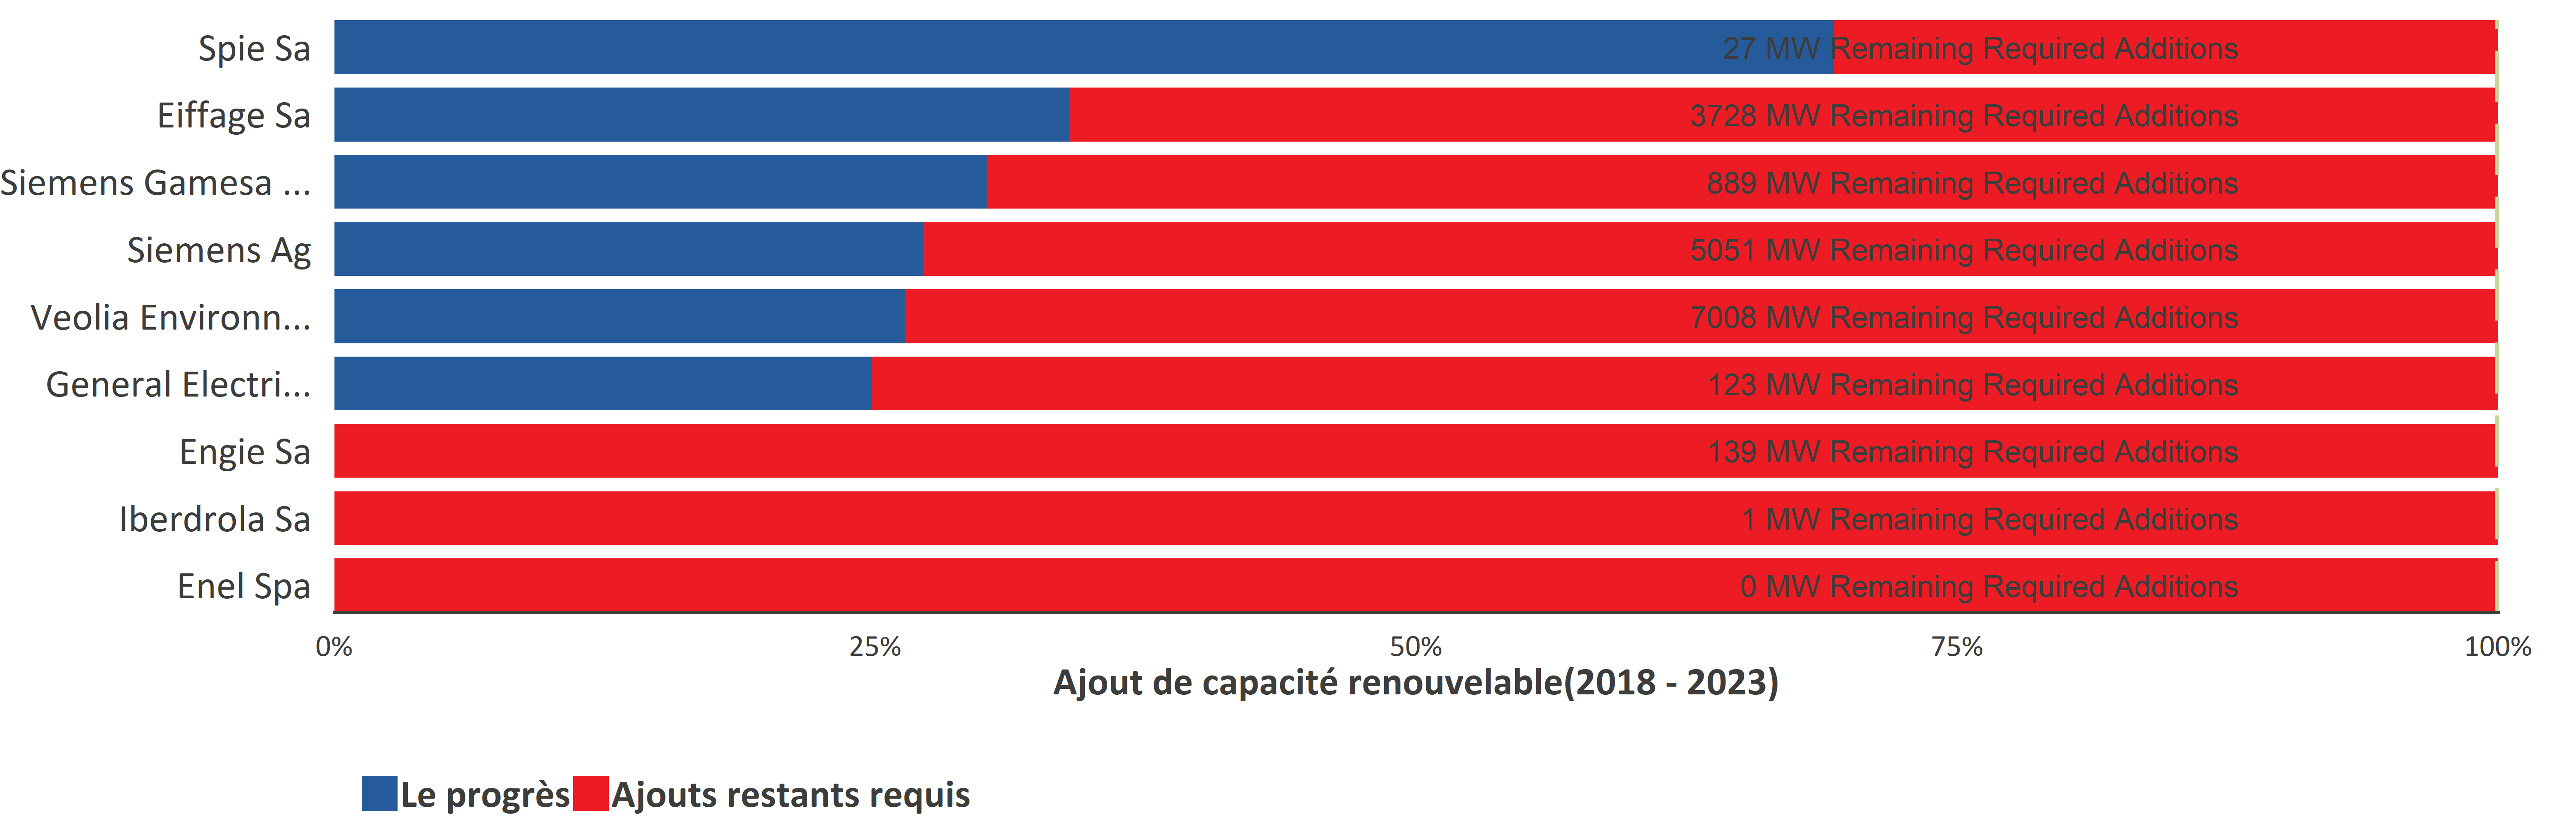
\includegraphics[trim = {0 0cm 0 0},width=1\linewidth]{ReportOutputs/Fig65}
	\end{center}
	%EQSpecificE
	
	%\PageFooterFifth
	\PageFooter{5 - EXPOSICIÓN DE LAS EMPRESAS}
	
	\newpage 
	%RenewableCapChartE
	%PowerSector_ALLE
	%CompanyChartsE
	
	

	\section*{} % 5th SECTION   
	\SectionHeadingDouble{SECCIÓN 6:}{ANÁLISIS DE EXPOSICIÓN }{DE BONOS SOBERANOS }

	\newpage
	\section*{} %
	\HeaderSingle{ANÁLISIS DE EXPOSICIÓN DE BONOS SOBERANOS }
	
	\begin{multicols}{2}
	
	\textbf{Los riesgos físicos y de transición pueden afectar la calificación crediticia y rendimientos de los bonos soberanos a través de los cambios en la fortaleza institucional, económica y fiscal de los países.} Los cambios en políticas pueden a su vez tener un impacto en la calidad crediticia a medida que los países fallen en fortalecer sus políticas de cambio climático. Ya se han realizado revisiones en las perspectivas de países que consideran cambios este tipo de políticas (e.g. S\&P en México debido a cambios en la política energética). Los cambios en la calificaciones y rendimientos podrían llevar eventualmente a una caída en el valor de las carteras de bonos soberanos y a un  posible riesgo de impago en el futuro. 
	
	
	\textbf{Los riesgos físicos} pueden afectar el valor de los bonos soberanos a través de un amplio conjunto de factores que influyen las calificaciones y, por lo tanto, los rendimientos, incluyendo:
	
		\begin{itemize}
	\item{\textbf{Fortaleza institucional} a través de la capacidad del gobierno para hacer frente a los daños en infraestructura, población desplazada, etc. Esta se ve afectada por fenómenos meteorológicos extremos, así como su capacidad de planificación ante cambios incrementales relacionados con el clima, como por ejemplo el aumento del nivel del mar.}
	\item{\textbf{Fortaleza económica } a través de la disminución de la actividad económica en sectores afectados por los efectos agudos e incrementales del cambio climático, que en consecuencia tiene un impacto en el PIB (Producto Interno Bruto).}
	\item{\textbf{Fortaleza fiscal }mediante el aumento del gasto (e.g. programas sociales, costos de reconstrucción y mitigación, costos de desplazamiento), menores ingresos fiscales debido a una menor actividad económica y un costo mayor de los préstamos.}
		\end{itemize}
	
	\textbf{Los riesgos de transición} pueden afectar igualmente el valor de los bonos soberanos.  Si una transición hacia una economía  baja en carbono no está bien diseñada y / o iniciada con suficiente antelación, esta puede traer graves consecuencias para la economía de un país, aunque en el largo plazo estas podrían ser menos severas que las consecuencias en caso de no tomarse medidas para mitigar el cambio climático.
	
	Las implicaciones crediticias se pueden reflejar en un amplio conjunto de factores que influyen las calificaciones de los bonos soberanos y, por lo tanto, en los rendimientos, incluyendo :
	
	
	
		\begin{itemize}
	\item{\textbf{Fortaleza institucional} a través de la capacidad de los gobiernos para construir políticas efectivas y previsibles. Una transición retrasada enfrentaría mayores desafíos en el diseño e implementación.}
	\item{\textbf{Fortaleza económica } a través de menores ingresos de sectores económicos de altas emisiones de carbono que afectan el PIB. La alta proporción en el PIB de sectores expuestos aumenta la susceptibilidad de los bonos soberanos a los riesgos de transición.} 
	\item{\textbf{Fortaleza fiscal }  a través de mayores (inversiones verdes, políticas sociales, etc.), menores ingresos fiscales debido a una menor actividad económica de sectores con altas emisiones de carbono y un mayor costo de los préstamos.}
		\end{itemize}
			
	\textbf{Gestión de riesgos climáticos.}La identificación de los tipos de riesgos relacionados con el clima a nivel de carteras y/o emisores y los factores que impulsan estos riesgos representan esencialmente el primer paso en la gestión de riesgos relacionados con el clima. Una vez identificadas estas vulnerabilidades, se debe pensar en las acciones climáticas para la mitigación de dichos riesgos. Generalmente, las principales acciones climáticas consideradas en las carteras de inversión son el ejercicio de la propiedad activa y la desinversión. La propiedad activa en bonos soberanos en temas climáticos es bastante limitada debido a las altas cargas asociadas a la cantidad de partes involucradas (por ejemplo, diferentes ministerios locales) y la divergencia de prioridades entre estas. A nuestro entender, no hay evidencia pública sobre los resultados del ejercicio de la propiedad activa con gobiernos en temas relacionados con el clima aparte de cuando se da en el contexto de una emisión de bonos verdes. Esta dinámica disminuye notablemente los potenciales de mitigación para esta clase de activo y, a menudo, empuja a los inversionistas hacia la venta de activos riesgosos, lo que conduce a una transferencia del riesgo en vez de su disminución.
	  
	
	
	\end{multicols}
	\PageFooter{6 -ANÁLISIS DE EXPOSICIÓN DE BONOS SOBERANOS }


	\newpage
	\section*{} %
	\HeaderSingle{ANÁLISIS DE EXPOSICIÓN  - RIESGOS FÍSICOS}
	
	\begin{multicols}{2}
		
		\textbf{Esta sección muestra la exposición de los emisores de la cartera de bonos soberanos hacia los riesgos físicos y riesgos de transición energética. Para los riesgos físicos, se utiliza como proxy la clasificación por país de Moody’s. Para los riesgos de transición se utiliza como proxy la dependencia del PIB a las industrias con alta intensidad de carbono y la base de activos físicos de los países emisores presentes en la cartera. Para contextualizar el análisis, se consideran los límites regulatorios locales en las inversiones internacionales en bonos soberanos, así como las vías disponibles para mitigar estos riesgos (e.g. Desinversión vs. Propiedad activa).}
		
	
	Existen dos canales por los cuales los riesgos físicos y de transición podrían afectar las carteras de bonos soberanos de las aseguradoras colombianas: i. cambios en la composición de la cartera para cumplir con los límites de inversión en caso de una descenso de la calificación; y / o ii. cambios en el valor de la cartera de bonos soberanos como consecuencia de una inadecuada valoración de los riesgos climáticos.
	 
La siguiente grafica muestra el desglose de la cartera de bonos soberanos por país y calificación crediticia. Estudios muestran que el impacto de los riesgos físicos y de transición podría causar una caída en la calificación entre uno y tres niveles debido a la dependencia a sectores con altas emisiones de carbono y de los efectos de eventos climáticos extremos (2ii 2019, S\&P 2015). Para poner esto en contexto, estimamos que una baja de uno o dos niveles implicaría que el sbdowngradeperc\% de la deuda internacional en su cartera tendría que ser redistribuida, mientras en el caso de la deuda colombiana ninguna redistribución sería necesaria.

		
		
		\textbf{Desglose de la cartera por país y calificación.}\\
		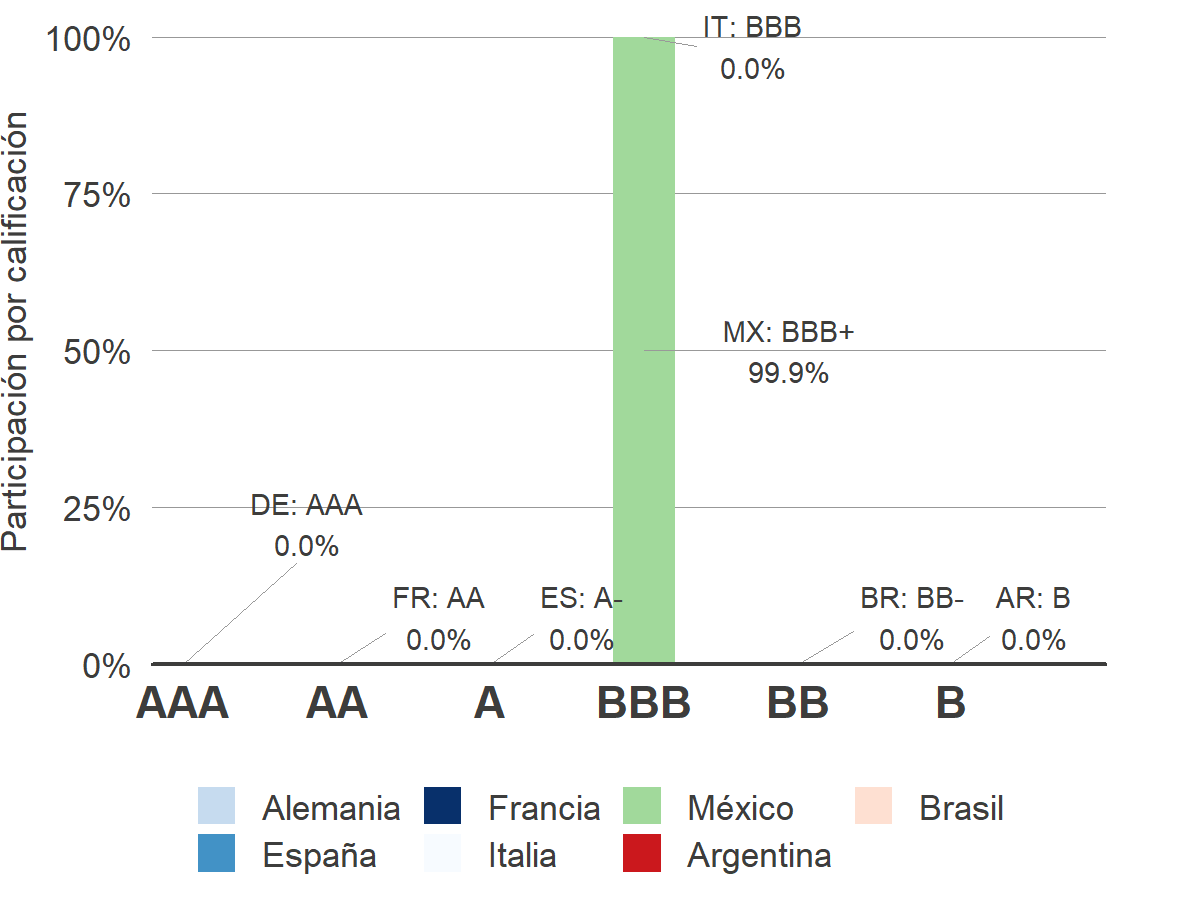
\includegraphics[trim = {0, 0, 0, 0cm},width=1\linewidth]{ReportOutputs/Fig91}
		
	La materialización de riesgos físicos y de transición, por lo tanto, podría tener un mayor impacto en términos de cambios en el valor de la cartera de bonos soberanos. El siguiente análisis muestra la exposición de los emisores de su cartera hacia los riesgos físicos y de transición.
	 
		
		\textbf{Riesgos físicos.} Actualmente no existen analíticas que cuantifiquen los cambios esperados en la calificación o rendimiento debido al cambio climático para los países presentes en la cartera, sin embargo, se puede lograr entender como los efectos del cambio climático afectan la susceptibilidad de los países utilizando un heatmap creado por Moody’s. En 2016, Moody’s evaluó los efectos físicos del cambio climático en emisores soberanos considerando cuatro canales primarios: i. el impacto económico potencial (e.g. una actividad más débil debido a una pérdida de producción agrícola); ii. daños en la infraestructura como resultado de la destrucción causada por eventos climáticos; iii. el aumento de los costos sociales (e.g. por problemas de seguridad alimentaria); y iv. desplazamientos de población debido a la migración forzada como resultado del cambio climático.
			
	La siguiente grafica muestra la exposición a riesgos físicos de la cartera. Esta considera el grado de exposición de cada país hacia eventos crónicos (e.g. aumentos de temperatura) y eventos agudos (e.g. sequías, incendios forestales) clasificando cada país desde más susceptibles a mucho menos susceptibles, y los activos bajo gestión en bonos soberanos en cada país.
	 
		
		
		\textbf{Susceptibilidad al impacto de cambio climático de la cartera de bonos soberanos}\\
		\includegraphics[trim = {0, 0, 0, 0cm},width=1\linewidth]{ReportOutputs/Fig92}
		
		
	\end{multicols}
	
	
	
	
	%\PageFooterFifth
\PageFooter{6 - ANÁLISIS DE EXPOSICIÓN DE BONOS SOBERANOS}
	
	\newpage
	\section*{} %
	\HeaderSingle{ANÁLISIS DE EXPOSICIÓN - RIESGOS DE TRANSICIÓN}
	
	
	\begin{multicols}{2}
	\textbf{Riesgos de transición.} Actualmente no existen analíticas para cuantificar cambios en la calificación o el rendimiento que puedan darse en la transición hacia una economía baja en carbono para los países dentro de la cartera (ver 2ii, 2019). Sin embargo, la susceptibilidad de estos países a una caída en la calificación debido a la transición puede evaluarse considerando la dependencia del PIB de países emisores presentes en la cartera a industrias con altas emisiones de carbono. El siguiente cuadro muestra el desglose del PIB (Producto Interno Bruto) de cada emisor por sector.	
	
		
		\textbf{Exposición del PIB a sectores de altas emisiones de carbono} \\
		\includegraphics[trim = {0, 0, 0, 0cm},width=1\linewidth]{ReportOutputs/Fig93}
	
	Las industrias de alta intensidad en carbono están propensas a verse afectadas por la transición energética. De hecho, una transición afectaría sus niveles de producción (e.g. menos petróleo será producido, menos vehículos de gasolina serán fabricados, etc.), los precios a los que venden sus productos y los gastos que deben soportar (e.g. altos valores del impuesto  al carbono, altos precios de las materias primas, etc.).
	
	La investigación realizada por 2Dii muestra que el sector petrolero en Sudamérica podría perder el 74\% de su valor agregado para 2040 (2ii, 2019).

	
	\textbf{Un análisis de exposición y crecimiento de tecnologías} proporciona información mas detallada sobre la susceptibilidad de los países hacia los riesgos de transición. Este permite entender si las economías están adaptando su combinación de tecnologías a la transición y a su vez disminuyendo/aumentando su producción de tecnologías de alto carbono/bajo carbono. La siguiente figura muestra la combinación de tecnologías y la producción actual y futura de combustibles fósiles, electricidad y automóviles. Los resultados son una función del peso de cada país emisor en su cartera y los planes de inversión y producción revelados por las empresas que producen en cada país. Los resultados se comparan con un escenario regional bajo una transición SDS en Startyear+5.
	
	
	
Los resultados muestran si las políticas actuales y las condiciones en el mercado local son suficientes para fomentar una transición ambiciosa. Una menor proporción de tecnologías bajas en carbono en Startyear+5 en comparación con la del escenario SDS implica que las políticas actuales y las condiciones del mercado no son lo suficientemente favorables para movilizar la industria a un escenario de 2\degree C.  
  
				
	\end{multicols}
	
		\begin{center}
		\includegraphics[trim = {0, 0, 0, 0cm},width=1\linewidth]{ReportOutputs/Fig94}
		\end{center}
	

	%\PageFooterFifth
\PageFooter{6 - ANÁLISIS DE EXPOSICIÓN DE BONOS SOBERANOS}

	\newpage
	
	
	
	\section*{} % 6th BACKGROUND
	\SectionHeading{SECCIÓN 7:}{BASES DEL MODELO}
	
	\newpage
	
	\section*{} % CONTEXT p7
	\HeaderSingle{CONTEXTO}
	
	\begin{multicols}{2}
		\textbf{Contexto:} En junio 2017, el grupo de trabajo sobre divulgación de información financiera relacionadas con el clima (TCFD) del consejo de estabilidad financiera del G20 recomendó a las instituciones financieras, realizar un análisis de escenario en sus carteras para evaluar los riesgos relacionados al cambio climático. El TCFD clasifico los riesgos ligados al cambio climático en dos tipos: riesgos físicos y riesgos de transición. Los riesgos de transición son aquellos riesgos generados por cambios en políticas, tecnologías, el mercado y regulaciones que probablemente acompañaran la transición hacia una economía baja en carbono. 
		
		
		\textbf{Objetivo:} El objetivo del análisis de escenarios es evaluar la exposición de los inversionistas al los riesgos de transición, mirando su exposición actual y futura estimada a actividades con altas y bajas en carbono. Este informe proporciona los resultados del análisis para una sola cartera.
		
		\textbf{Alcance:} Los elementos clave del análisis son:
		
		\begin{itemize}
			\item{\textit{Producción planeada y actual y tendencias de inversión.} La producción actual y producción planeada (sector de combustibles fósiles y automotriz), la capacidad instalada actual y las adiciones de capacidad (sector eléctrico) en los próximos 5 años fueron obtenidas por medio de bases de datos de proveedores comerciales de inteligencia de mercado. Estos proveedores de datos suministran información prospectiva de producción y capacidad de activos físicos, incluyendo barriles de petróleo por campo petrolero, automóviles por modelo y empresa, y nueva capacidad por central eléctrica. 2Dii asocia estos datos con sus propietarios directos y sus casas matrices para obtener el “perfil de producción” actual para cada empresa en cada tecnología. Estos planes de producción están asociados a los activos financieros (acciones y bonos corporativos) emitidos por la empresa. La base de datos de activos físicos utilizada en este análisis ha sido obtenida por medio de proveedores de información en diciembre de 2018. Para más información sobre la interpretación de la base datos del sector eléctrico, diríjase a la sección “Consideraciones y limitaciones importantes”.}
			
			\item{\textit{Asignando la producción de activos físicos a activos financieros.} En base a la proporción de acciones o deuda total retenida en una cartera, el modelo asigna a la cartera una parte de los planes de producción actuales de cada empresa en cada tecnología. El agregado del conjunto de empresas en la cartera representa el “perfil de producción actual” de la cartera en cada tecnología. A su vez, esto describe la “exposición” actual en cada tecnología.}
			
			\item{\textit{Desde escenarios de nivel macro hasta objetivos de nivel micro. }Para calcular niveles de producción consistentes con un escenario climático como los escenarios de la AIE, el modelo utiliza el principio de parte justa (“Fair Share”), el cual aplica los cambios especificados por el escenario en una tecnología y región determinada de manera equitativa para todos los propietarios de activos físicos en cada tecnología en la región concerniente. Esto crea un conjunto de alternativas de prospectivas de producción y perfiles de capacidad coherentes con el escenario para cada empresa y tecnología. Estos perfiles alternativos son luego agregados a nivel de cartera para construir el “perfil de producción objetivo” de la cartera en el escenario. Este perfil es utilizado para determinar la “exposición objetivo” del inversionista a una tecnología en el escenario. La “exposición objetivo” no asume cambios en la composición de la cartera, esta modela cambios requeridos en planes de producción e inversión en las diferentes empresas en la cartera a fin de hacerlos coincidir con el despliegue de cada tecnología descrito en el escenario. } 
			
			\item{\textit{El análisis de intensidad de emisiones} se realiza en sectores para los que no existe suficiente información disponible sobre los activos físicos, los escenarios o cuando no existe una tecnología baja en carbono de reemplazo comercialmente disponible. Para estos sectores, los esfuerzos de descarbonización se limitará en el desarrollo de métodos de producción y uso más eficientes, así como en inversiones para investigación y desarrollo en los próximos 5 a 10 años, a fin de traer alternativas neutras en CO\textsubscript{2} a nivel comercial a mediano plazo. Como consecuencia, los escenarios y los datos son relativamente imprecisos.}
				\end{itemize}
		
		\textbf{Resultados de análisis de escenario:} El “perfil objetivo” de la cartera bajo el escenario puede compararse con los planes de producción e inversión actualmente revelados de la cartera para cada tecnología a fin de derivar la exposición a riesgos de transición, así como la medida en que se proyecta que la cartera aumente o disminuya su alineación con el ScenarioValue durante los próximos 5 años.
		\newline
		
	\end{multicols}
			
\PageFooter{7 - BASES DEL MODELO}			
			
	\newpage
	
	
		
	\section*{} % BACKGROUND TO THE MODEL
	\HeaderSingle{BASES DEL MODELO}
	
	\begin{multicols}{2}
		
		
		\textbf{Evaluación de la alineación con la trayectoria de transición del ScenarioValue.} Este análisis evalúa el nivel de alineación con la trayectoria de transición del ScenarioValue, utilizando dos referencias:
		
		\begin{itemize}
			\item{\textit{La cartera en la transición del ScenarioValue.} Se refiere al perfil de producción objetivo de la cartera bajo el ScenarioValue: esta muestra los cambios requeridos en el perfil de producción de las empresas en la cartera, a fin de cumplir los objetivos en base a la metodología descrita. Dado que los títulos y su peso en la cartera son idénticos para la cartera y sus versiones alternativas, la comparación muestra que tan alineados o desalineados están los perfiles de producción actuales de cada empresa de la cartera con cada escenario.}
			\item{\textit{El mercado ScenarioValue.} Este es el perfil de producción objetivo del mercado acorde al ScenarioValue. El principio anteriormente descrito es aplicado a una cartera alineada representada por un índice. Debido a que los títulos y su peso en la cartera de mercado difieren con aquellos de la cartera global, esta comparación remarcara la alineación o desalineación “idiosincrática”. En otras palabras, muestra como la composición actual de la cartera afecta la alineación con los diferentes escenarios, cuando la primera  referencia solo tiene énfasis en los cambios requeridos por parte de las empresas.}
		\end{itemize}
		
		
	La alineación o desalineación de la producción de una cartera y de la exposición de cada tecnología relativa a un escenario es una manera para comprender mejor la exposición de un inversionista a los riesgos de transición energéticos. Si los cambios de políticas, tecnologías, mercados o regulaciones se producen para acercar la economía global al ScenarioValue, la desalineación de una tecnología en particular probablemente afectaría los rendimientos financieros asociados a los activos físicos subyacentes. Sin embargo, este análisis solo analiza una dimensión de los riesgos de transición energética: los activos a riesgo en la economía real. Esta, no toma en cuenta la resiliencia financiera de la empresa hacia esos cambios y su capacidad de adaptarse, lo cual requeriría un análisis financiero mas profundo.
		
		\textbf{Escenarios.} El análisis de escenario tiene como base los escenarios desarrollados por la AIE. El escenario Beyond 2 Degrees (B2DS) se enfoca en lograr un crecimiento sostenible, y al mismo tiempo, limita el aumento de temperatura por debajo de 2\degree C. El escenario Sustainable Development (SDS) es un avance hacia un enfoque holístico de la sostenibilidad, en lugar de enfocarse solamente en el cambio climático. Además del escenario SDS, la AIE también define el escenario New Policy (NPS) y el Current Policity (CPS). Los escenarios proveen proyecciones prospectivas con detalles regionales suficientes para desarrollar un análisis de escenario para once tecnologías en tres sectores.
		
			El modelo utiliza los siguientes indicadores provenientes de los escenarios de la AIE con el que se compara la cartera:
	
		\begin{itemize}
			\item{Capacidad eléctrica por combustible expresada en MW (e.g. renovables, acero, gas, petróleo, nuclear);;}
			\item{Producción petrolera expresada en barriles/año;}
			\item{Producción de gas expresada en m\textsuperscript{3} /año;}
			\item{Producción de carbón expresada en toneladas/ año;}
			\item{Trayectoria de emisión de gases de efecto invernadero en algunos de sectores suplementarios (e.g. Aviación, transporte marítimo, cemento, acero).}
		\end{itemize}
		
		 
		\textbf{Datos de activos físicos. } Los datos sobre los activos físicos vienen de los siguientes proveedores de data:
		\begin{itemize}
			\item{GlobalData (data de centrales eléctricas incluyendo centrales clasificadas como activas, anunciadas, financiadas, parcialmente activas, temporalmente inactivas, bajo construcción, bajo rehabilitación o modernización; data de producción de petróleo y gas y sus proyecciones a 2019-2024, así como data de minería de carbón); }
			\item{WardsAuto (vehículos ligeros de pasajeros, incluyendo proyecciones BAU Startyear-Startyear+5); }
			\item{Blomberg (data financiera);}
			\item{S\&P Cross Reference Services (base de datos que permite mapea los títulos financieros con sus casas matrices);}
			\item{Morningstar (base de dato de fondos). }
			
		\end{itemize}
		
		\textbf{Parámetros del modelo.} El análisis de escenario presentado refleja una selección de parámetros de entrada.  Mas detalles sobre estos parámetros y las diferentes implicaciones de la especificación de estos pueden ser encontrados en www.transitionmonitor.com/backgroundinformation.
		
		
		
	\end{multicols}
\PageFooter{7 - BASES DEL MODELO}
	
	
	\newpage
	
	\section*{} % BACKGROUND TO THE MODEL
	\HeaderDouble{CONSIDERACIONES IMPORTANTES Y LIMITACIONES}{ AL INTERPRETAR ESTOS RESULTADOS }
	
	\begin{multicols}{2}
		\begin{itemize}
			\item{\textit{Rigurosidad de los escenarios.} El uso de un escenario dado (B2DS, SDS, NPS, CPS) no constituye un supuesto de que este escenario sea más probable que algún otro. Igualmente, la selección de los escenarios de la AIE no debe ser interpretada como una aprobación de los supuestos subyacentes por parte de 2Dii. La AIE ha históricamente asumido valores importantes de energía nuclear y captura de carbón en sus escenarios, un supuesto que es continuamente debatido por la comunidad científica. Además, la comunidad internacional ha acelerado su objetivo global de 2\degree C a muy por debajo de 2\degree C y hacia 1.5\degree C. Es importante destacar que cada inversionista puede y podrá querer adoptar una opinión individual sobre un escenario de descarbonización que puede o no estar ligado a los escenarios modelados por la AIE.}
			
			\item{\textit{Una fotografía instantánea en lugar de pronósticos.} La data prospectiva de producción está basada en los planes actuales “revelados” por parte de las empresas, y está sujeta a cambios. Los resultados no deben ser interpretadas como predicciones, sino más bien como las estimaciones de los planes actuales de las empresas a partir de varias fuentes de información proporcionadas por expertos de inteligencia de mercado en cada industria. Dado el horizonte de 5 años, es probable que estos planes cambien de alguna manera en el curso de los años. Igualmente, es muy probable que los inversionistas alteren la composición de su cartera a lo largo del tiempo. La maduración de bonos corporativos es de generalmente de 3 a 7 años. La duración promedio de retención de una acción por un administrador de fondos ese de 20 meses. Sin embargo, este análisis busca ser una evaluación puntual de las exposiciones futuras bajo las condiciones actuales. }
			
			\item{\textit{Proyecciones del sector de energía.} A diferencia de la data de producción para los combustibles fósiles y el sector automotriz. Los datos de capacidad del sector de electricidad no incluyen información acerca de los retiros planeados. Por consiguiente, esta data debe ser interpretada como una medida de la capacidad “encerrada” actualmente y no como un pronóstico de la capacidad futura. Los retiros no son incluidos debido a varias razones. Primero, la disponibilidad de datos sobre los retiros varía significativamente en las distintas jurisdicciones y regiones, en la medida en que la no inclusión de información sobre los retiros se consideró más representativa de la capacidad respecto a la inclusión de datos parciales. Segundo, en contraste con el sector de combustibles fósiles donde los pozos petroleros, yacimientos de gas o carbón cesan su producción cuando sus recursos se agotan, las centrales eléctricas pueden anunciar su retiro, o incluso estar retiradas y luego reanudar su producción. Dado el alto nivel de incertidumbre en retiros planeados, estos no son incluidos en las proyecciones del sector eléctrico, por consiguiente, las proyecciones de capacidad deben ser interpretadas como el potencial “encerrado” máximo de la infraestructura actual. Para las tecnologías proyectadas a disminuir bajo el ScenarioValue, la brecha entre las proyecciones de capacidad actual y la capacidad coherente con el ScenarioValue deben ser consideradas como un estimado de la capacidad que debe ser retirada para alinearse con el ScenarioValue} 
			
			\item{\textit{Capacidad para capturar estrategias de ISR.} El modelo se apoya sobre una “cartera de mercado” diversificada enfocado en tecnologías claves reflejadas en las hojas de ruta de la AIE. Por ende, las carteras temáticas invertidas en tecnologías innovadoras y/o carteras de ISR con consideraciones ambientales, sociales y gubernamentales pueden no tener en cuenta estos elementos.}
			
		\end{itemize}
		
		
	\end{multicols}
	\PageFooter{7 - BASES DEL MODELO}

	\newpage		
	
	\section*{} % CONTEXT p8
	\HeaderSingle{RIESGOS DE TRANSICIÓN PARA LOS INVERSIONISTAS}
	\begin{multicols}{2}
	\textbf{¿Que son los riesgos de transición?} Los riesgos de transición pueden definirse en términos generales como los riesgos económicos y financieros asociados a la transición a una economía de bajo carbono. La comunidad internacional ha definido un mandato para limitar la contribución del hombre al calentamiento global a menos de 2\degree C por encima de los niveles preindustriales. Según las bases científicas disponibles, lograr este objetivo requiere la descarbonización de la economía en el curso de este siglo. Está previsto que esta descarbonización tendrá repercusiones importantes para los sectores de alto carbono. Destacando los sectores de combustibles fósiles, energía y transporte, los cuales representan la mayor parte de emisiones antropogénicas de CO\textsubscript{2} a nivel mundial.
		
	A medida que la economía se descarboniza, las empresas que no se anticipen adecuadamente a la transición serán susceptibles a estar expuestas a riesgos económicos. Por otro lado, las empresas que se preparen bien para esta transición estarán preparadas para capitalizar esta oportunidad económica. Igualmente, los riesgos económicos podrían traducirse en riesgos financieros en los mercados financieros si estos riesgos no son adecuadamente anticipados para los actores del mercado financiero. 
		
	Crucialmente, está previsto que una transición hacia una economía de bajo carbono tendrá efectos dramáticos a corto y mediano plazo. Para el año 2040, en 21 años solamente, la producción global de carbón esta prevista a disminuir un 46\%, con una previsión de decrecimiento más acelerada en mercados desarrollados. La capacidad de generación eléctrica a base de carbón deberá disminuir un 41\% en el mundo. La producción de vehículos de gasolina y diésel esta prevista a disminuir un 21\%. Este declive en las actividades de alto carbono vendrá acompañado con una reducción proporcional de emisiones a causa del despliegue y crecimiento de nuevas tecnologías. La capacidad de energías renovables y la producción de vehículos eléctricos esta prevista a cuadriplicarse en volumen para el año 2040.
		
	Un análisis de escenario puede ayudar a las instituciones financieras a evaluar y, a fin de cuentas, a gestionar los riesgos y oportunidades asociados a la transición. En reconocimiento de esos riesgos, los análisis de escenarios han sido implementados por centenas de instituciones y supervisores financieros hasta la fecha. Esto constituye la base de las recomendaciones del TCFD. El TCFD señala que “las evaluaciones prospectivas de asuntos climáticos son importantes para inversionistas y otros actores para comprender el nivel de vulnerabilidad de las organizaciones frente a los riesgos de transición y físicos, así como la manera en que estas vulnerabilidades se manifiestan y como deben ser atendidas. Como resultado, el TCFD está convencido que las organizaciones deberán utilizar análisis de escenarios para evaluar las implicaciones comerciales, estratégicas y financieras eventuales de riesgos ligados al clima y sus oportunidades y de igual manera, revelarlos, según corresponda, en su reporte financiero anual" (TCFD Final Report, p. 33).
		
	Para aclarar sus recomendaciones sobre el análisis de escenario, el TCFD explica que “Un tipo clave de escenario de riesgo de transición es el llamado escenario de 2\degree C, que presenta una trayectoria de emisiones consistente con mantener el aumento de temperatura promedio mundial a 2\degree C por encima de los niveles preindustriales.” (TCFD Final Report, p. 35).
		
	Partiendo de esta premisa, el presente reporte destaca los siguientes puntos para la cartera: 1) la exposición actual a los riesgos de transición en los sectores de combustibles fósiles, electricidad y sector automotriz; 2) las tendencias sectoriales de la cartera relativa a un escenario de 2\degree C a lo largo del tiempo; y 3) la exposición futura esperada en base a esas tendencias. 
		
	Si bien estos sectores no representan todas las actividades ni todos los sectores de alto carbono, estos sectores representan la mayor parte en una cartera típica promedio y la contribución más significativa al cambio climático en la actualidad.
		
	Este reporte no realiza estimaciones especificas en cuanto a la perdida potencial de valor en las carteras si estos riesgos se materializan, lo cual esta obviamente asociado a un sinfín de supuestos de modelización e incertidumbres significativas. Para cualquier valor individual, la perdida potencial puede variar de 0 a 100\% e incluso puede estar asociada con retornos positivos, dependiendo de la capacidad de adaptación de la empresa, la anticipación de las tendencias de los mercados financieros, y la naturaleza de una posible revaloración. Este reporte busca contribuir a la anticipación adecuada de estos riesgos la cual minimiza la perdida.
		
	\end{multicols}

	\PageFooter{7 - BASES DEL MODELO}

	\newpage
	\section*{} % UNDERSTANDING THE POWER SECTOR
	\HeaderSingle{ENTENDIENDO EL SECTOR ELÉCTRICO }	
	
	
	\begin{multicols}{2}
		
	El análisis de la cartera de generación eléctrica se basa en las proyecciones prospectivas de las adiciones de capacidad por tipo de combustible en los próximos 5 años en base a la data suministrada por GlobalData. El horizonte temporal de 5 años corresponde al horizonte de planeación de inversiones en adiciones de capacidad de producción de electricidad promedio, reconociendo que los horizontes de planeación para inversiones especificas pueden ser más largos o más cortos. Por lo tanto, un análisis a mayor plazo no permitiría identificar nuevas adiciones relevantes que estén actualmente en la cartera de planeación de las empresas. Igualmente, se excluyen de las graficas de las empresas, las adiciones de capacidad de generación de electricidad planeadas por empresas fuera del sector de generación eléctrica (por ejemplo, compañías de tecnología de informació (TI, por sus siglas en inglés) que construyen parques eólicos para alimentar sus instalaciones). La evaluación de la cartera es en base de las adiciones de capacidad planeada por las empresas que poseen los títulos en las carteras, ponderadas por su peso relativo en la cartera. 
		
	Es importante señalar que los datos oficialmente anunciados o planeados de retiros de activos físicos no son considerados en este análisis. Esto es intencional, dada la escasez de datos, así como el deseo de mostrar los retiros requeridos. Para las tecnologías proyectadas a disminuir bajo el ScenarioValue, la brecha entre la proyección de capacidad actual y la capacidad consistente con el ScenarioValue debe ser interpretado como una estimación de la capacidad que debe ser retirada para estar alineada con el ScenarioValue.
		
	Como se mencionó anteriormente, los escenarios se basan en tendencias globales escaladas a las carteras en base al principio de parte justa “Fair Share”, donde la tendencia del macro-escenario es transformada a micro-objetivos en función de la proporción del mercado de la cartera. Para el sector de electricidad, este enfoque no toma en cuenta variaciones en el mercado a través de las diferentes clases de activos y actores, especialmente con el aumento de capacidad de energía renovable de los hogares (e.g. paneles solares de techo), los cuales llevan a cambios en el mercado de energía. Si bien esta tendencia implica que en la práctica las empresas serán susceptibles a perder parte de su mercado, esta tendencia no se internaliza intencionalmente en el análisis a fin de documentar la perdida potencial de participación en el mercado bajo el ScenarioValue - y, por ende, el riesgo potencial de transición acumulado. 
		
	En un escenario de 2\degree C o inferior, el sector de electricidad se descarbonizará a largo plazo por medio de la transición de una producción a base energías fósiles hacia una producción a base de energías renovables. La Agencia Internacional de Energía (AIE) establece que en un escenario de 2\degree C:
		
	"El suministro de electricidad mundial está llamado a diversificarse y descarbonizarse, en donde la generación de electricidad por fuentes de bajo carbono sustituye al carbón antes del 2020. Se proyecta que la participación de la generación a carbón en la generación caerá de más del 40\% ahora al 28\% en 2040. Para entonces, las energías renovables basadas en energía eólica, solar y bioenergía incrementarán su participación en el mercado del 6\% a 20\%”. (AIE World Energy Outlook 2016, p. 241).
		
	La combinación de tecnologías variara considerablemente según el escenario. La generación de energía a base de carbón aumentará según las tendencias actuales, pero disminuirá en un escenario de 2\degree C. Asimismo, la energía eólica y solar incrementará más rápidamente en un escenario de 2\degree C.
		
	Las inversiones en bonos corporativos y acciones están expuestas a estas tendencias a través de los títulos financieros emitidos por empresas de electricidad. Un estimado de 28\% de los activos relacionados a generación de energía son propiedad de empresas listadas en bolsa y 19\% de los activos son propiedad de entidades estadales listadas en bolsa, como por ejemplo, emisores de bonos municipales. (Ver gráfica siguiente).
		
		
	\end{multicols}
	
	\begin{multicols}{2}
		
		\vspace{-.2cm}
		\textbf{Combinación de tecnologías bajo BAU de la AIE y escenario 2DS para ciertas tecnologías. }
		
		
		
		
		\adjincludegraphics[width = .95\linewidth,trim={0cm 0cm 0cm .5cm},clip]{ReportGraphics/PowerLine_ES.png}
		
		\textit{\small Fuente: IEA World Energy Outlook 2016
		}
		
		\textbf{Tenencia de los activos de energía a nivel global}
		\newline
		
		\adjincludegraphics[width = .8\linewidth,trim={0cm 0cm 0cm 0.5cm},clip]{ReportGraphics/PowerPie_ES.png}
		
		\textit{\small Fuente: IEA analysis and 2Dii, based on Platts, Bloomberg Professional service, Bloomberg New Energy Finance and national sources
		}
		
	\end{multicols}

	\PageFooter{7 - BASES DEL MODELO}			
	\newpage
	
	\section*{} % EMISSIONS INTENSITY ANALYSIS
	\HeaderSingle{ANÁLISIS DE INTENSIDAD DE EMISIONES}
	
	\begin{multicols}{2}
		
		
	\textbf{Metodología}
		
	Para el análisis de intensidad de emisiones, un factor de emisión por cada planta es calculado en unidades por producción.  Luego, este valor es agregado a la cartera ponderando la participación de la empresa en la cartera. La data del escenario se escala a este punto de partida y la trayectoria de las reducciones de emisiones se indica para los próximos 5 años. 
		
	Estos resultados pueden servir como un punto de partida para discusiones con las empresas de acero, cemento, aviación y transporte marítimo sobre sus estrategias para lograr la trayectoria de cada sector.
		
			
	\textbf{Escenarios} 
		
	La trayectoria de reducción de la intensidad de emisiones se basa en los escenarios presentados en el Energy Technology Perspectives 2017. La producción y emisión esperada para los sectores de acero, cemento y aviación son suministrados a nivel regional. Las trayectorias presentadas en estos sectores siguen un escenario de 2\degree C. Por otra parte, el sector de transporte marítimo no dispone de data suficiente para hacer esto, por consecuencia esta cartera es comparada con el mercado.
		
		
	\textbf{Acero} 
		
	Después de la producción de químicos, la producción de acero representa el segundo proceso que consume más energía entre los sectores industriales y el sector de mayor intensidad de carbono. El despliegue de hornos de arco eléctrico es clave para reducir las emisiones del sector (incluso si esta tecnología sigue emitiendo de carbono). El cálculo de los factores de emisión para cada planta de acero se basa en la tecnología utilizada, el combustible utilizado, y los factores regionales de la red eléctrica y el consumo de combustible. Adicionalmente, este valor es multiplicado por la capacidad de la planta y un factor de capacidad a nivel regional seleccionado. Este factor es suministrado por las bases de datos de la OCDE y la Asociación Mundial de Acero.
		
	\textbf{Cemento}
		
	La producción de cemento representa igualmente uno de los procesos con más emisiones entre los sectores industriales.  Se espera que la producción de concreto represente el 5\% de las emisiones antropogénicas (Cement Sustainability Initiative). Esto concierne principalmente la producción de tres fuentes distintas: el proceso de calcinación, el consumo de energía térmica y el uso de electricidad. El factor de emisión es calculado a partir de factores regionales aplicados a cada planta. La mayoría de estos datos provienen de Cement Sustainability Initiative.
	
	\textbf{Aviación}
		
	Para estimar las emisiones actuales de CO\textsubscript{2} de la flota de aviones se realizaron supuestos en cuento a las tasas de utilización de las aeronaves. Las emisiones han sido estimadas para cada empresa usando como base los kilómetros por pasajeros; una metodología equivalente fue calculada para las aeronaves de carga. Existe un alto nivel de incertidumbres en esta metodología.
		
	\textbf{Transporte marítimo}
		
	La mejor manera para evaluar la sostenibilidad del transporte marítimo es en base a el Carbon Efficiency Level, desarrollado por el Carbon War Room y Rightship. Cada barco es clasificado de A a G, donde A representa el barco más eficiente en cada categoría de barco (e.g. petrolero, carga, etc.), lo que permite un punto de comparación común. La clasificación se calcula dinámicamente para tener en cuenta las mejoras anuales en eficiencia y las variaciones en la media, de modo que los barcos A siempre representan el 10\% superior (medido en términos de intensidad de CO\textsubscript{2}). Como no hay datos disponibles del escenario, los resultados de envío de la cartera se comparan con el mercado.
			
			
			
	\end{multicols}	
	\PageFooter{7 - BASES DEL MODELO}

	\newpage
	
	
	\section*{} % NOTES AND DISCLAIMER
	\HeaderSingle{NOTAS}
	
	\begin{multicols}{2}
	Las bases de datos y escenarios para este análisis son proporcionados en esta sección.
		
	\textbf{Investigaciones publicadas}
		
	La metodología detrás de este análisis de escenario, los criterios de contabilidad, y la información específica de los escenarios y datos se puede encontrar en los siguientes documentos de investigación.
		
	Criterios de contabilidad: http://www.mdpi.com/2071-1050/ 10/2/328 
		
	Escenarios: http://et-risk.eu/toolbox/ scenarios/ 
		
	Análisis de datos a nivel de activos físicos: http://2degrees-investing.org/ IMG/pdf/assetdata\_v0.pdf
		
	\textbf{Fuentes para datos y análisis de escenarios}
		
	Data del sector automotriz de julio 2017 es suministrada por WardsAuto/ AutoForecastSolutions. Data del sector de la energía es de julio 2017 y es suministrada por GlobalData. Para acoplar los datos activos con sus empresas, la data es usada por los proveedores mencionados anteriormente y cuando sea posible, complementada con información de empresas a partir de Bloomberg. Toda la data financiera, así como los números de identificación para asociar los instrumentos financieros con las empresas son extraídos de Bloomberg.
		
	Las trayectorias de carbonización para otros sectores son extraídas de Science-Based Targets Initiative, la cual fundamenta sus metodologías en los escenarios de la AIE World Energy Outlook 2016. Debido a que este reporte no incluye data de escenario para el sector automotriz, la data relacionada es obtenida a partir del reporte equivalente “Energy Technology Perspective Report de World Energy Outlook”. Los puntos de referencias (Benchmarks) para el sector de electricidad son obtenidos regionalmente y aplicados en relación a la data de exposición regional, y luego agregados y ponderados de acuerdo a la exposición regional de la cartera. Los otros resultados son globales.
		
	\textbf{Fuentes}
		
	2ii (2019) https://2degrees-investing.org/wp-content/uploads/
	2019/02/Stress-test-report\_final.pdf
	Cement Sustainability Initiative (2018) https://www.wbcsd cement.org/index.php/key-issues/climate-protection
		
	Energy Technology Perspectives 2017 (2018) https://www.iea.org /etp/
		
	IPCC (2018) https://www.ipcc.ch/report/ar5/
		
	FSB (2018) https://www.fsb-tcfd.org/publications/final-recommendations-report/
		
	WoodMackenzie (2018) https://www.woodmac.com/news/ editorial/carbon-intensity-not-all-assets-are-created-equal/ 
		
	World Energy Outlook 2017 (2018) https://www.iea.org/weo2017/
	
	\end{multicols}
	
	\PageFooter{7 - BASES DEL MODELO}	
	\newpage

	
\end{document} 

